% NOTA 13/07/17
% Estou escrevendo esta nota aqui por ser mais simples. Até agora tive a dúvida de que símbolos usar em relação a produtórios e somatórios. Resolvi usar um + grande para somatório e um \times grande para produtório quando se tratam de operações binárias em grupos e aneis, etc... No entanto, também existem o produto (Cartesiano) de grupos, os produtos de espaços topológicos e os produtos e somas diretas em estruturas algébricas. Pelo que li hoje, esses não têm muito a ver com as operações binárias (talvez algumas propriedade semelhante...). O produto, de modo geral, é o produto categórico. A soma direta é um caso mais específico e nem sempre é o coproduto categórico, mas esses detalhes não entendi muito e não pretendo tratar no livro (por enquanto). Eu deve então definir dois símbolos para produto. Um para produtório e outro para o produto de conjuntos, grupos, aneis... Acho que posso manter as operações binárias como \bigplus e \bigtimes (e mudar a aparência do símbolo que esses comandos produzem) e definir um novo comando para o produto no sentido de conjuntos e estruturas em geral, pois esse é o produto topológico.

\part{Álgebra}

\chapter{Operações Binárias e Estruturas Básicas}

A \emph{Álgebra} estuda objetos matemáticos conhecidos como \emph{estruturas algébricas}. As definições desse objeto variam e podem ser tomadas de modo a serem mais ou menos gerais. No entanto, esse objetivos sempre são n-listas em que as entradas são conjuntos e funções. Uma das definições que podem ser tomadas é a de que essas estruturas são listas em que a primeira entrada é um conjunto e as demais são funções. Em geral, essas funções são \emph{operações $n$-árias}, funções da $n$-ésima potência de um conjunto nele mesmo. Não definiremos aqui esses objetos com detalhes, nos restringindo somente a casos específicos. Ao leitor fica a oportunidade de perceber as semelhanças entre as definições e generalizá-las, ou mesmo de procurar mais a respeito.

\section{Operações Binárias}

\begin{defi}
Seja $X$ um conjunto não vazio. Uma \emph{operação binária} em $X$ é uma função
	\begin{align*}
	\func{\opb}{X \times X}{X}{(x_1,x_2)}{x_1 \opb x_2}.
	\end{align*}
\end{defi}

\begin{prop}[Propriedade de fecho]
\label{prop:restri.op.bin}
Sejam $X$ e $Y$ conjuntos não vazios tais que $Y \subseteq X$ e $ \opb $ uma operação binária em $X$. Então a restrição $ \opb |_{Y \times Y}$ da operação binária $ \opb $ a $Y \times Y$ é uma operação binária em $Y$ se, e somente se, para todos $y_1,y_2 \in Y$
	\begin{equation*}
	y_1 \opb y_2 \in Y.
	\end{equation*}
\end{prop}
\begin{proof}
Basta notar que, como $Y \subseteq X$, então $Y \times Y \subseteq X \times X$, e a proposição segue da proposição \ref{conj:prop.func.rest.ig}.
\end{proof}

Denotamos $\opb |_{Y \times Y}$ por $\opb$ quando não há ambiguidade.

\begin{defi}
Seja $X$ um conjunto. Uma operação binária \emph{associativa} é uma operação binária $\opb: X \times X \to X$ que satisfaz, para todos $x_1,x_2,x_3 \in X$,
	\begin{equation*}
	(x_1 \opb x_2) \opb x_3 = x_1 \opb (x_2 \opb x_3).
	\end{equation*}
Uma operação binária \emph{comutativa} é uma operação binária $\opb : X \times X \to X$ que satisfaz, para todos $x_1,x_2 \in X$
	\begin{equation*}
	x_1 \opb x_2 = x_2 \opb x_1.
	\end{equation*}
\end{defi}

\begin{defi}
	Sejam $X$ um conjunto e $+$ uma operação binária em $X$. Uma operação binária \emph{distributiva} sobre $+$ é uma operação binária $\times$ em $X$ que satisfaz, para todos $x_1,x_2,x_3 \in X$,
	\begin{equation*}
	x_1 \times (x_2 + x_3) = (x_1 \times x_2) + (x_1 \times x_3).
	\end{equation*}
\end{defi}

\section{Magma}

\begin{defi}
Um \emph{magma} é um par $\bm X=(X,\opb)$ em que $X$ é um conjunto não vazio e $ \opb $ é uma operação binária em $X$.
\end{defi}

\begin{defi}[Identidade]
Seja $\bm X=(X, \opb )$ um magma. Uma \emph{identidade} com respeito a $\opb$ é um elemento $\id \in X$ que satisfaz, para todo $x \in X$,
	\begin{equation*}
	\id \opb x = x = x \opb \id.
	\end{equation*}
\end{defi}

Pode-se distinguir \emph{identidade à esquerda} e \emph{identidade à direita}, que seria o caso de $e$ se só satisfizesse, respectivamente, as igualdades da esquerda e da direita acima, mas não adotaremos essa distinção neste livro.

\begin{prop}
\label{prop:unic.elem.neut}
Seja $\bm X = (X, \opb )$ um magma. Se existe identidade com respeito a $\opb$, ela é única.
\end{prop}
\begin{proof}
Suponha que existam duas identidades com respeito a $\opb$, $\id_1$ e $\id_2$. Então
	\begin{align*}
	\id_1 = \id_1 \opb \id_2 = \id_2.
	\end{align*}
\end{proof}

\begin{defi}[Operação com conjuntos]
Sejam $\bm X$ um magma, $A,B \subseteq X$ e $x \in X$. Definimos
	\begin{align*}
	x \opb A &:= \set{x \opb a}{a \in A} \\
	A \opb x &:= \set{a\opb x}{a \in A} \\
	A \opb B &:= \set{a \opb b}{a \in A,b \in B}.
	\end{align*}
\end{defi}

\section{Semigrupo}

\begin{defi}
Um \emph{semigrupo} é um magma $\bm X=(X,\opb)$ em que $\opb$ é associativa. Um semigrupo \emph{comutativo} é um semigrupo em que $\opb$ é comutativa.
\end{defi}

\begin{defi}
Seja $\bm X=(X,\opb)$ um semigrupo, $n \in \N^*$ e $(x_i)_{i \in [n]}$ elementos de $X$. O \emph{operatório} desses elementos é
	\begin{equation*}
	\bigopb _{i \in [n]} x_i :=
		\begin{cases}
		x_0, & n=1\\
		x_{n-1} \opb \displaystyle \bigopb_{i \in [n-1]} x_i, & n>1.
		\end{cases}
	\end{equation*}
\end{defi}

\begin{nota}
Costumamos denotar essa operação por
	\begin{equation*}
	x_{n_1} \opb \cdots \opb x_0 := \bigopb_{i \in [n]} x_i = (x_{n-1} \opb ( \cdots (x_1 \opb x_0)))
	\end{equation*}
\end{nota}

O símbolo usado para a soma $+$ é o \emph{somatório} $\displaystyle\bigplus$ e o símbolo usado para o produto $\times$ é o \emph{produtório} $\displaystyle\bigtimes$. Essa definição considera que as operações vão sendo feitos à esquerda, mas uma mesma definição poderia ter sido feita para operações à direita --- todas demonstrações ainda valeriam, considerando que as as ordens fossem devidamente trocadas.

\begin{prop}
Sejam $\bm X=(X,\opb)$ um semigrupo, $n,k \in \N^*$ e $(x_i)_{i \in [n+k]}$ elementos de $X$. Então
	\begin{equation*}
	\bigopb_{i \in [n+k]} x_i = \bigopb_{i \in [k]} x_{n+i} \opb \bigopb_{i \in [n]} x_i.
	\end{equation*}
\end{prop}
\begin{proof}
A demonstração será por indução em $k$. Se $k=1$, por definição segue que
	\begin{equation*}
	\bigopb_{i \in [n+1]} x_i = x_{n} \opb \displaystyle \bigopb_{i \in [n]} x_i = \bigopb_{i \in [1]} x_{n+i} \opb \bigopb_{i \in [n]} x_i.
	\end{equation*}
Considere agora que vale a igualdade para algum $k \in \N^*$. Então
	\begin{align*}
	\bigopb_{i \in [n+k+1]} x_i
		&= x_{n+k} \opb \bigopb_{i \in [n+k]} x_i \\
		&= x_{n+k} \opb \left(\bigopb_{i \in [k]} x_{n+i} \opb \bigopb_{i \in [n]} x_i\right) \\
		&= \left(x_{n+k} \opb \bigopb_{i \in [k]} x_{n+i} \right) \opb \bigopb_{i \in [n]} x_i \\
		&= \bigopb_{i \in [k+1]} x_{n+i} \opb \bigopb_{i \in [n]} x_i. \qedhere
	\end{align*}
\end{proof}

\begin{prop}[Associatividade Generalizada]
Sejam $\bm X=(X,\opb)$ um semigrupo, $n \in \N^*$, $(x_i)_{i \in [n]}$ elementos de $X$ e $(k_j)_{j \in [p]}$ uma partição de $[n]$ (ou seja: $n = \sum_{j \in [p]} k_j$ e, para todos $j \in [p]$, $k_j \neq 0$). Então
	\begin{equation*}
	\bigopb_{i \in [n]} x_i = \bigopb_{j \in [p]}\left(\bigopb_{i \in [k_j]} x_{i + k_0 + \cdots + k_{j-1}}\right).
	\end{equation*}
\end{prop}
\begin{proof}
Segue por indução da proposição anterior.
\end{proof}

Essa proposição diz que podemos colocar os parêntesses como quisermos que o resultado será o mesmo, pois
	\begin{equation*}
	\bigopb_{j \in [p]}\left(\bigopb_{i \in [k_j]} x_{i + k_0 + \cdots + k_{j-1}}\right) = \left(\bigopb_{i \in [k_{p-1}]} x_{i + k_0 + \cdots + k_{p-2}}\right) \opb \cdots \opb \left(\bigopb_{i \in [k_0]} x_i\right)
	\end{equation*}
e a partição $(k_j)_{j \in [p]}$ determina essa separação.

\begin{prop}[Comutatividade Generalizada]
Sejam $\bm X=(X, \opb )$ um semigrupo comutativo e $n \in \N^*$. Então, para toda bijeção $\psi\colon [n] \to [n]$,
	\begin{equation*}
	\bigopb_{i \in [n]} x_{\psi(i)} = \bigopb_{i \in [n]} x_i.
	\end{equation*}
\end{prop}
\begin{proof}
Usaremos o fato de que $\opb$ é associativa. A demonstração será por indução em $n$. Se $n=1$, a afirmação é óbvia. Considere que vale para algum $n \in \N^*$ e seja $\psi\colon [n+1] \to [n+1]$ uma bijeção. Definamos $k = \psi\inv(n)$ e a bijeção
	\begin{align*}
	\func{\phi}{[n]}{[n]}{i}{
		\begin{cases}
		\psi(m) 		& i<k \\
		\psi(m+1) & i>k.
		\end{cases}
	}
	\end{align*}
Da associatividade generalizada, da comutatividade e da hipótese para $n$, segue que
	\begin{align*}
	\bigopb_{i \in [n+1]} x_{\psi(i)}
		&= \bigopb_{i \in [n-k]} x_{\psi(i+k+1)} \opb x_{\psi(k)} \opb \bigopb_{i \in [k]} x_{\psi(i)} \\
		&= x_{n} \opb \bigopb_{i \in [n-k]} x_{\psi(i+k+1)} \opb \bigopb_{i \in [k]} x_{\psi(i)} \\
		&= x_{n} \opb \bigopb_{i \in [n-k]} x_{\phi(i+k)} \opb \bigopb_{i \in [k]} x_{\phi(i)} \\
		&= x_n \opb \bigopb_{i \in [n]} x_{\phi(i)}\\
		&= x_n \opb \bigopb_{i \in [n]} x_i \\
		&= \bigopb_{i \in [n+1]} x_i. \qedhere
	\end{align*}
\end{proof}

\section{Homomorfismo de Semigrupos}

\begin{defi}
Sejam $\bm X_1=(X_1,\opb_1)$ e $\bm X_2=(X_2,\opb_2)$ semigrupos. Um \emph{homomorfismo de semigrupos} de $\bm X_1$ para $\bm X_2$ é uma função $h: X_1 \to X_2$ que satisfaz, para todos $x,x' \in X_1$
	\begin{equation*}
	h(x  \opb_1  x')=h(x') \opb_2 h(x').
	\end{equation*}
\noindent Denota-se $h: \bm X_1 \to \bm X_2$. %e o conjunto de todos esses homomorfismos de semigrupos é denotado por $\homo(\bm X_1,\bm X_2)$.
\end{defi}

\begin{prop}[Composição de homomorfismos]
\label{comp.hom.sem}
Sejam $\bm X_1=(X,\opb_1)$, $\bm X_2=(X_2,\opb_2)$ e $\bm X_3=(X_3,\opb_3)$ semigrupos e $h_1: \bm X_1 \to \bm X_2$ e $h_2: \bm X_2 \to \bm X_3$ homomorfismos de semigrupos. Então $h_2 \circ h_1: \bm X_1 \to \bm X_3$ é homomorfismo de semigrupos.
\end{prop}
\begin{proof}
Sejam $x,x' \in X_1$. Então
	\begin{align*}
	(h_2 \circ h_1)(x \opb_1 x') &= h_2(h_1(x \opb_1 x')) \\
		&= h_2(h_1(x) \opb_2 h_1(x')) \\
		&= h_2(h_1 (x)) \opb_3 h_2(h_1(x')) \\
		&= (h_2 \circ h_1)(x) \opb_3 (h_2 \circ h_1)(x').
	\end{align*}
\end{proof}

\section{Monoide}

\begin{defi}
Um \emph{monoide} é uma tripla $\bm M=(M,\opb,\id)$ em que $(M,\opb)$ é um semigrupo e $\id$ é uma identidade com respeito a $\opb$. Um monoide \emph{comutativo} é um monoide cuja operação binária $\opb$ é comutativa.
\end{defi}

\begin{nota}
Denotaremos a identidade de um monoide $\bm M$ por $\id_M$ quando houver ambiguidade. Ainda, como existe identidade, definimos
	\begin{equation*}
	\bigopb_{i \in [0]} x_i = \id.
	\end{equation*}
\end{nota}

\begin{ex}
O conjunto $\N$, com a operação binária
	\begin{align*}
	\func{\max}{\N^2}{\N}{(n,n')}{\max\{n,n'\}}
	\end{align*}
e a identidade $0$, formam um monoide comutativo.
\end{ex}

\begin{defi}[Inverso]
Sejam $\bm X = (X, \opb )$ um magma, $\id$ uma identidade com respeito a $\opb$ e $x \in X$. Um \emph{inverso} de $x$ com respeito a $\opb$ e $\id$ é um elemento $\bar x \in X$ que satisfaz
	\begin{equation*}
	\overline x \opb x = \id =  x \opb \overline x.
	\end{equation*}
Uma operação unária \emph{inversa} com respeito a $\opb$ e $\id$ é uma operação unária
	\begin{align*}
	\func{\inv}{X}{X}{x}{x\inv}
	\end{align*}
tal que, para todo $x \in X$, $x \inv$ é o inverso de $x$ com respeito a $\opb$ e $\id$.
\end{defi}

Pode-se distinguir \emph{inverso à esquerda} e \emph{inverso à direita}, que seria o caso de $\bar x$ se só satisfizesse, respectivamente, as iguadades da esquerda e da direita acima, mas não adotaremos essa distinção neste livro.

\begin{prop}
\label{prop:unic.inv}
Seja $(M,\opb,\id)$ um monoide. Se $m \in M$ tem inverso com respeito $\opb$ e $\id$, ele é único.
\end{prop}
\begin{proof}
Suponha que existam dois inversos $\overline m$ e $\overline{\overline m}$ de $m$. Então
	\begin{equation*}
	\overline m = \overline m \opb \id = \overline m \opb (m \opb \overline{\overline m}) = (\overline m \opb m) \opb \overline{\overline m} = \id \opb \overline{\overline m} = \overline{\overline m}. \qedhere
	\end{equation*}
\end{proof}

\begin{nota}
A unicidade do inverso nos permite denotar o inverso de um elemento $m \in M$ de algum modo fixo. Quando a operação binária é a adição ($+$), denotamos o inverso por $-m$; quando é a multiplicação ($\times$, $\cdot$, $\circ$), denotamo-lo por $m\inv$.
\end{nota}

\begin{prop}
Seja $(M,\opb,\id)$ um monoide. Se $m \in M$ tem inverso com respeito a $\opb$ e $\id$, então $m\inv$ tem inverso e
	\begin{equation*}
	(m\inv)\inv=m.
	\end{equation*}
\end{prop}
\begin{proof}
	\begin{equation*}
	\begin{split}
	(m\inv)\inv &= (m\inv)\inv  \opb  e \\
		&= (m\inv)\inv  \opb  (m\inv  \opb  m) \\
		&= ((m\inv)\inv  \opb  m\inv)  \opb  m \\
		&= e  \opb  m \\
		&= m.
	\end{split}
	\end{equation*}
\end{proof}

\begin{defi}
Seja $\bm M=(M,\opb,\id)$ um monoide. Um \emph{submonoide} de $\bm M$ é um monoide $\bm S=(S,\opb _S,\id_S)$ em que $S \subseteq M$, $\opb _S= \opb |_{S \times S}$ e $\id_S=\id$. Denota-se $\bm S \leq \bm M$. Um submonoide \emph{próprio} de $\bm M$ é um monoide $\bm S \leq \bm M$ em que $S$ é um subconjunto próprio de $M$ ($S \subset M$). Denota-se $\bm S < \bm M$.
\end{defi}

\begin{prop}
\label{alge:prop.submon}
Sejam $\bm M=(M,\opb,\id)$ um monoide e $S \subseteq M$ um conjunto tal que
	\begin{enumerate}
	\item (Identidade) $\id \in S$.
	\item (Fechamento) Para todos $s_1,s_2 \in S$, $s_1 \opb s_2 \in S$;
	\end{enumerate}
\noindent
Então $\bm S=(S,\opb|_{S \times S},\id)$ é um monoide. Ainda, se $\bm M$ é comutativo, então $\bm S$ é comutativo.
\end{prop}
\begin{proof} Por simplicidade, definamos $\star :=  \opb _{S \times S}$.

%($\Rightarrow$) Suponhamos que $\bm S$ é um monoide com $\id \in S$. (Identidade) Então vale a identidade. (Fechamento) Como $\bm S$ é um monoide, $\star$ é uma operação binária, portanto segue a propriedade de fechamento (\ref{prop:restri.op.bin}).

%($\Leftarrow$)
Suponhamos que valem as propriedades listadas. (Operação binária) Pela identidade, segue que $S \neq \emptyset$, e disso e do fechamento, segue que $\star$ é uma operação binária (\ref{prop:restri.op.bin}).
(Associatividade) Sejam $s_1,s_2,s_3 \in S$. Da associatividade de $ \opb $ segue que
	\begin{equation*}
	 (s_1 \star s_2) \star s_3 = (s_1  \opb  s_2)  \opb  s_3 = s_1  \opb  (s_2  \opb  s_3) = s_1 \star (s_2 \star s_3).
	 \end{equation*}
Logo $\star$ é associativa. (Identidade) Seja $s \in S$. Como $\id \in S$, da identidade de $ \opb $ segue que
	\begin{equation*}
	\id \star s = \id  \opb  s = s = s \opb  \id = s \star \id.
	\end{equation*}
Logo $\id$ é identidade de $\bm S$.

Por fim, suponhamos que $\bm M$ é um monoide comutativo. Sejam $s_1,s_2 \in S$. Como $ \opb $ é comutativa, então
	\begin{equation*}
	s_1 \star s_2 = s_1  \opb  s_2 = s_2  \opb  s_1 = s_2 \star s_1.
	\end{equation*}
Logo $\star$ é comutativa.
\end{proof}

Vale observar que, somente sabendo que $\bm S$ é um monoide, isto é, que um subconjunto $S$ de um monoide $\bm M$ com a operação do monoide restrita a esse subconjunto formam um monoide, não podemos garantir que a identidade de $\bm S$ é a mesmo que a de $\bm M$.

\section{Homomorfismos de Monoides}

\begin{defi}
Sejam $\bm M_1=(M_1,\opb_1,\id_1)$ e $\bm M_2=(M_2,\opb_2,\id_2)$ monoides. Um \emph{homomorfismo de monoides} de $\bm M_1$ para $\bm M_2$ é uma função $h: M_1 \to M_2$ que satisfaz
	\begin{enumerate}
	\item $h$ é um homomorfismo de semigrupos de $\bm M_1$ para $\bm M_2$:
		\begin{enumerate}
		\item para todos $m,m' \in M_1$, $h(m \opb_1 m')=h(m) \opb_2 h(m')$;
		\end{enumerate}
	\item $h(\id_1)=\id_2$.
	\end{enumerate}
\noindent Denota-se $h: \bm M_1 \to \bm N_2$. %e o conjunto de todos esses homomorfismos de monoides é denotado por $\homo(\bm M_1,\bm M_2)$.
\end{defi}

Podemos notar que precisamos garantir que a função $h$ leve a identidade de um monoide para a identidade de outro, já que isso não seria verdade se função fosse somente um homomorfismo de semigrupos. No entanto, mesmo sem a segunda propriedade, um homomorfismo de semigrupos entre grupos garante que a imagem da identidade do primeiro é a identidade do conjunto imagem. Veremos mais adiante que um homomorfismo de grupos é simplesmente um homomorfismo de semigrupos, pois ele é suficiente para preservar a estrutura algébrica de grupos.

\begin{prop}[Composição de homomorfismos]
\label{comp.hom.mon}
Sejam $\bm M_1=(M_1,\opb_1.\id_1)$, $\bm M_2=(M_2,\opb_2,\id_2)$ e $\bm M_3=(M_3,\opb_3,\id_3)$ monoides e $h_1: \bm M_1 \to \bm M_2$ e $h_2: \bm M_2 \to \bm M_3$ homomorfismos de monoides. Então $h_2 \circ h_1: \bm M_1 \to \bm M_3$ é homomorfismo de monoides.
\end{prop}
\begin{proof}
	\begin{enumerate}
	\item Como homomorfismos de monoides são homomorfismos de semigrupos, o resultado segue da proposição na seção de semigrupos que afirma que composição de homomorfismos é homomorfismo (\ref{comp.hom.sem}).
	\item Para mostrar que a identidade é preservada, basta notar que
	\begin{equation*}
	(h_2 \circ h_1)(\id_1) = h_2(h_1(\id_1)) = h_2(\id_2) = \id_3.
	\end{equation*}
	\end{enumerate}
\end{proof}


\chapter{Grupos}

\section{Construções Algébricas}

\subsection{Grupo e Subgrupo}

%\begin{defi}
%	Um \emph{grupo} é um monoide $\bm G=(G, \opb )$ em que todos elementos de $G$ têm inverso sob $ \opb $. Um grupo \emph{comutaivo} é um grupo em que $ \opb $ é comutativa.
%\end{defi}

%\begin{defi}
%Um \emph{grupo} é uma quádrupla $\bm G=(G,\opb,\id,\inv)$ em que $(G,\opb,\id)$ é um monoide e $\inv: G \to G$ é uma operação unária inversa com respeito a $\opb$ e $\id$.
%\end{defi}

\begin{defi}
Um \emph{grupo} é uma quádrupla $\bm G=(G,\opb,\id,\inv)$ em que $G$ é um conjunto, $\opb : G \times G \to G$ é uma operação binária associativa, $\id \in G$ é uma identidade com respeito a $\opb$ e $\inv: G \to G$ é uma operação unária inversa com respeito a $\opb$ e $\id$; isto é, satisfazem
	\begin{enumerate}[label=\textbf{G\arabic*.},ref={G\arabic*}]
	\item \label{G1}(Associatividade) Para todos $g_1,g_2,g_3 \in G$,
		\begin{equation*}
		(g_1 \opb g_2) \opb g_3 = g_1 \opb (g_2 \opb g_3);
		\end{equation*}
	\item \label{G2} (Identidade) Para todo $g \in G$,
		\begin{equation*}
		\id \opb  g = g =g  \opb \id;
		\end{equation*}
	\item \label{G3} (Invertibilidade) Para todo $g \in G$,
		\begin{equation*}
		g\inv \opb g = \id = g \opb g\inv.
		\end{equation*}
	\end{enumerate}
\noindent
Um grupo \emph{comutativo} é um grupo cuja operação $\opb$ é comutativa; isto é, satisfaz
	\begin{enumerate}[label=\textbf{G\arabic*.},ref={G\arabic*}]
	\setcounter{enumi}{3}
	\item \label{G4} (Comutatividade) Para todos $g_1,g_2 \in G$,
	\begin{equation*}
	g_1 \opb g_2 = g_2 \opb g_1.
	\end{equation*}
	\end{enumerate}
Denota-se $g_1 \opb g_2$ por $g_1g_2$. Quando o grupo é comutativo, podemos usar $+$ para denotar sua operação binária. Nesse caso, o inverso de $g \in G$ é denotado por $-g$.
\end{defi}

Em vista das definições introdutórias do capítulo anterior, um \emph{grupo} é uma quádrupla $\bm G=(G,\opb,\id,\inv)$ em que $(G,\opb,\id)$ é um monoide e $\inv: G \to G$ é uma operação unária inversa com respeito a $\opb$ e $\id$.

\begin{defi}
Sejam $\bm G=(G,\opb)$ um grupo, $g \in G$ e $n \in \N$. Definimos
	\begin{equation*}
	g^n := \bigopb_{i=1}^n g \e g^{-n} := \bigopb_{i=1}^n g^{-1}.
	\end{equation*}
\end{defi}

\begin{prop}[Leis de corte e inversão]
	Seja $\bm G$ um grupo. Então
	\begin{enumerate}
	\item $\forall g,g_1.g_2 \in G \qquad gg_1 = gg_2 \quad \Rightarrow \quad g_1 = g_2$.
	\item $\forall g,g_1.g_2 \in G \qquad g_1g = g_2g \quad \Rightarrow \quad g_1 = g_2$.
	\item $\forall g_1,\ldots,g_n \in G \qquad (g_1 \cdots g_n)^{-1}=g_n^{-1} \cdots g_1^{-1}.$
	\end{enumerate}
\end{prop}
\begin{proof}
	Se $g g_1 = g g_2$, então
	\begin{equation*}
	g_1 = (g^{-1}g)g_1 = g^{-1}(gg_1) = g^{-1}(gg_2) = (g^{-1}g)g_2 = g_2.
	\end{equation*}
A demonstração da segunda implicação é análoga.
\end{proof}

\begin{defi}
Seja $\bm G=(G,\opb,\id,\inv)$ um grupo. Um \emph{subgrupo} de $\bm G$ é um grupo $\bm S=(S,\opb_S,\id_S,{}^{-1_S})$ em que $S \subseteq G$, $\opb_S=\opb|_{S \times S}$, $\id_S=\id$ e $\inv = {}^{-1_S}$. Denota-se $\bm S \leq \bm G$. Um subgrupo \emph{próprio} de $\bm G$ é um subgrupo $\bm S \leq \bm G$ em que $S$ é um conjunto próprio de $G$ ($S  \subset G$). Denota-se $\bm S < \bm G$.
\end{defi}

\begin{prop}
\label{alge:prop.subgru}
Sejam $\bm G$ um grupo e $S \subseteq G$ que satisfaz
	\begin{enumerate}[label=\textbf{SG\arabic*.},ref={SG\arabic*}]
	\item \label{SG1} (Não-vacuidade) $S \neq \emptyset$;
	\item \label{SG2} (Fechamento) Para todos $s_1,s_2 \in S$, $s_1s_2 \in S$;
	\item \label{SG3} (Invertibilidade) Para todo $s \in S$,  $s\inv \in S$.
	\end{enumerate}	
\noindent
Então $\bm S=(S,\opb|_{S \times S})$ é um grupo. Ainda, se $\bm G$ é comutativo, então $\bm S$ é comutativo.
\end{prop}
\begin{proof}
Por simplicidade, definamos $\star := \opb|_{S \times S}$.

%($\Rightarrow$) (\ref{SG1}) Como $\bm S$ é um grupo, $e \in S$, portanto $S \neq \emptyset$.
%(\ref{SG2}) Como $\bm S$ é grupo, $\star$ é uma operação binária, portanto segue que, para todo $s_1,s_2 \in S$, $s_1s_2 \in S$ (\ref{prop:restri.op.bin}).
%(\ref{SG3}) Seja $s \in S$. Como $\bm S$ é grupo, existe $s^{-1} \in S$ inverso de $s$ em $\bm S$. Como $s^ {-1} \in G$, segue da unicidade do inverso que $s^{-1}$ é o inverso de $s$ em $\bm G$.

%($\Leftarrow$)
(Operação binária) Pela primeira e segunda propriedades de $S$, segue que $\star$ é uma operação binária (\ref{prop:restri.op.bin}).
(\ref{G1}) Sejam $s_1,s_2,s_3 \in S$. Então
	\begin{equation*}
	(s_1 \star s_2) \star s_3 = (s_1 \opb s_2) \opb s_3 = s_1 \opb (s_2 \opb s_3) = s_1 \star (s_2 \star s_3).
	\end{equation*}
(\ref{G2}) Como $S \neq \emptyset$, existe $s \in S$, portanto $s\inv \in S$. Isso implica que $\id=s \opb s\inv \in S$ e, como $\id$ é identidade de $\bm G$, segue que, para todo $s \in S$,
	\begin{equation*}
	\id \star s = \id \opb s = s = s \opb \id = s \star \id.
	\end{equation*}
(\ref{G3}) Seja $s \in S$. Pela terceira propriedade de $S$, segue que o inverso de $s$ em $\bm G$ pertence a $S$. Então
	\begin{equation*}
	s\inv \star s = s\inv \opb s = e = s \opb s\inv = s \star s\inv,
	\end{equation*}
portanto $s\inv$ é o inverso de $s$ em $\bm S$.

(\ref{G4}) Por fim, suponhamos que $\bm G$ é um grupo comutativo. Sejam $s_1,s_2 \in S$. Como $\opb$ é comutativa, então
	\begin{equation*}
	s_1 \star s_2 = s_1 \opb s_2 = s_2 \opb s_1 = s_2 \star s_1.
	\end{equation*}
\end{proof}

\begin{prop}
Sejam $\bm G$ um grupo e $\mathcal G$ o conjunto dos subgrupos de $\bm G$. Então $(\mathcal G,\leq)$ é um conjunto parcialmente ordenado.
\end{prop}
\begin{proof}
Claramente, $\bm G \in \mathcal G$, portanto $\mathcal G$ não é vazio. Mostremos que $\leq$ é uma ordem parcial em $\mathcal G$. (Reflexividade) Seja $\bm S \in \mathcal G$. Então $\bm S \leq \bm S$, pois $\bm S$ é um grupo, $S \subseteq S$ e $\opb|_{S \times S} = \opb|_{S \times S}$. (Antissimetria) Sejam $\bm{S_1},\bm{S_2} \in \mathcal G$ tais que $\bm{S_1} \leq \bm{S_2}$ e $\bm{S_2} \leq \bm{S_1}$. Então $S_1 \subseteq S_2$ e $S_2 \subseteq S_1$, o que implica $S_1=S_2$, e portanto $\opb|_{S_1 \times S_1} = \opb|_{S_2 \times S_2}$, o que implica $\bm{S_1} = \bm{S_2}$. (Transitividade) Sejam  $\bm{S_1},\bm{S_2},\bm{S_3} \in \mathcal G$ tais que $\bm{S_1} \leq \bm{S_2}$ e $\bm{S_2} \leq \bm{S_3}$. Então $S_1 \subseteq S_2$ e $S_2 \subseteq S_3$, o que implica $S_1 \subseteq S_3$ e, portanto, $\opb_{S_1} = \opb|_{S_3 \times S_3}$.
\end{proof}

\begin{prop}
\label{alge:prop.subgru.triv}
Seja $\bm G$ um grupo. Então $\bm{\{\id\}}$ e $\bm G$ são subgrupos de $\bm G$.
\end{prop}

\begin{prop}
\label{alge:prop.subgru.inter}
Sejam $\bm G$ um grupo, $(\bm S_i)_{i \in I}$ uma família de subgrupos de $\bm G$ e
	\begin{equation*}
	S := \bigcap_{i \in I} S_i.
	\end{equation*}
Então $\bm S$ é um subgrupo de $\bm G$.
\end{prop}
\begin{proof}
(\ref{SG1}) Para todo $i \in I$, $\bm{S_i}\leq \bm G$, portanto $e \in N_i$. Logo $e \in N$. (\ref{SG2}) Sejam $s_1, s_2 \in S$. Para todo $i \in I$, $s_1,s_2 \in S_i$. Como $\bm{S_i} \leq \bm G$, segue que $s_1s_2 \in S_i$, o que implica que $s_1s_2 \in S$. (\ref{SG3}) Seja $s \in S$. Para todo $i \in I$, $s \in S_i$ e, como $\bm{S_i} \leq \bm{G}$, segue que $s^{-1} \in S_i$, o que implica que $s^{-1} \in S$.
\end{proof}

\begin{prop}
\label{alge:prop.subgru.uni}
Sejam $\bm G$ um grupo, $(\bm S_i)_{i \in I}$ uma família superiormente dirigida de subgrupos de $\bm G$ (para todos $i_1,i_2 \in I$, existe $i \in I$ tal que $S_{i_1} \subseteq S_i$ e $S_{i_2} \subseteq S_i$) e
	\begin{equation*}
	S := \bigcup_{i \in I} S_i.
	\end{equation*}
Então $\bm S$ é um subgrupo de $\bm G$.
\end{prop}
\begin{proof}
(Não-vacuidade) Para todo $i \in I$, $\bm{S_i}\leq \bm G$, portanto $e \in N_i$. Logo $e \in N$. (Fechamento) Sejam $s_1,s_2 \in S$. Existem $i_1,i_2 \in I$ tais que $s_1 \in S_{i_1}$ e $s_2 \in S_{i_2}$ e, pela propriedade, existe $i \in I$ tal que $S_{i_1} \subseteq S_{i} \e S_{i_2} \subseteq S_{i}$. Então $s_1,s_2 \in S_i$. Como $\bm{S_i} \leq \bm G$, segue que $s_1s_2 \in S_i$, o que implica que $s_1s_2 \in S$. (Invertibilidade) Seja $s \in S$. Existe $i \in I$ tal que $s \in N_i$ e, como $\bm{S_i} \leq \bm G$, segue que $s^{-1} \in S_i$, o que implica que $s^{-1} \in S$.
\end{proof}

A propriedade definida acima é equivalente a dizer que a família $(S_i)_{i \in I}$ é um conjunto dirigido com respeito a $\subseteq$.

\begin{defi}
	Seja $\bm M$ um monoide. O conjunto dos elementos invertíveis de $M$ é denotado por $M^*$.
\end{defi}

O asterisco não tem a ver com a operação $\opb$ do monoide.

\begin{prop}
Seja $\bm M = (M,\opb,\id)$ um monoide. Então existe uma operação unária $\inv: M^* \to M^*$ tal que $\bm{M^*}=(M^*,\opb|_{M^* \times M^*},\id,\inv)$ é um grupo.
\end{prop}
\begin{proof}
	Sejam $m_1,m_2 \in M^*$. Então existem $m_1^{-1},m_2^{-1} \in M$ tais que
	\begin{equation*}
	m_1m_1^{-1}=\id \e m_2m_2^{-1}=\id.
	\end{equation*}
Portanto
	\begin{equation*}
	(m_1m_2)(m_2^{-1}m_1^{-1}) = m_1(m_2m_2^{-1})m_1^{-1} = m_1m_1^{-1} = id,
	\end{equation*}
o que mostra que $m_1m_2 \in M^*$. Ainda, note que $\id \in M^*$, pois $\id \opb \id = \id$. Como $M^*$ é contém a identidade e fechado sob $\opb$, segue que $(M^*,\opb,\id)$ é um monoide (\ref{alge:prop.submon}). Por fim, $\bm{M^*}$ é um grupo pois, por definição, todo elemento tem inverso e ele é único.
\end{proof}

\begin{defi}
Sejam $\bm G$ um grupo e $g \in G$. A \emph{conjugação} por $g$ é a função
	\begin{align*}
	\func{C_g}{G}{G}{h}{ghg\inv}.
	\end{align*}
A \emph{translação à direita} por $g$ é a função
	\begin{align*}
	\func{D_g}{G}{G}{h}{hg}.
	\end{align*}
A \emph{translação à esquerda} por $g$ é a função
	\begin{align*}
	\func{E_g}{G}{G}{h}{gh}.
	\end{align*}
\end{defi}

\subsection{Coclasses e Índice de Subgrupo}

\begin{defi}
Sejam $\bm G$ um grupo, $\bm S \leq \bm G$ um subgrupo e $g \in G$. A \emph{coclasse à esquerda} de $\bm S$ em $\bm G$ com \emph{representante} $g$ é o conjunto
	\begin{equation*}
	gS := \{gs:s \in S\}.
	\end{equation*}
A \emph{coclasse à direita} de $\bm S$ em $\bm G$ com \emph{representante} $g$ é o conjunto
	\begin{equation*}
	Sg := \{sg:s \in S\}.
	\end{equation*}
\end{defi}

Coclasses também são conhecidas como classes laterais. As definições de coclasses à esquerda ou à direita são análogas e, por consequência, toda definição ou proposição envolvendo uma das duas tem uma definição ou proposição dual envolvendo a outra. Por esse motivo, durante este capítulo consideraremos sempre coclasses à esquerda.

\begin{prop}
\label{alge:prop.gru.coclas}
Sejam $\bm G$ um grupos, $\bm S \leq \bm G$ um subgrupo e $g_1g_2 \in G$. Então
	\begin{enumerate}
	\item $g_1(g_2S) = (g_1g_2)S \e (Sg_1)g_2 = S(g_1g_2)$
	\item $g_1S=g_2S \Leftrightarrow g_2^{-1}g_1 \in S$ e $Sg_1=Sg_2 \Leftrightarrow g_2^{-1}g_1 \in S$.
	\end{enumerate}
\end{prop}
\begin{proof}
	\begin{enumerate}
	\item ($\subseteq$) Seja $g \in g_1(g_2S)$. Existem $g' \in g_2S$ tal que $g=g_1g'$ e, portanto, existe $s \in S$ tal que $g'=g_2s$. Mas então, pela associatividade, $g=g_1(g_2s) = (g_1g_2)s$, e segue que $g \in (g_1g_2)S$.
($\supseteq$) Seja $g \in (g_1g_2)S$. Então existe $s \in S$ tal que $g=(g_1g_2)s$ e, da associatividade, segue que $g=g_1(g_2s)$, logo $g \in g_1(g_2S)$. A outra igualdade é análoga.
	
	\item ($\Leftarrow$) Seja $g \in g_1S=g_2S$. Então existem $s,s' \in S$ tais que $g=g_1s=g_2s'$, logo $g_2^{-1}g_1=s's^{-1}$. Como $\bm S$ é subgrupo, segue que $g_2^{-1}g_1=s's^{-1} \in S$.

\noindent
($\Rightarrow$) ($\subseteq$) Se $g_2^{-1}g_1 \in S$, existe $s \in S$ tal que $g_2^{-1}g_1=s$, portanto $g_1=g_2s$, logo $g_1 \in g_2S$. Assim, dado $g \in g_1S$, existe $s' \in S$ tal que $g=g_1s'$. Como $\bm S$ é subgrupo, $ss' \in S$, logo $g=g_2ss' \in g_2S$. ($\supseteq$) Da mesma forma, como $\bm S$ é subgrupo, $g_1^{-1}g_2=(g_2^{-1}g_1)^{-1}=s^{-1} \in S$, o que implica que $g_2=g_1s^{-1} \in g_1S$. Assim, dado $g \in g_2S$, existe $s' \in S$ tal que $g=g_2s'$. Como $\bm S$ é subgrupo, $s^{-1}s' \in S$, logo $g=g_1s^{-1}s' \in g_2S$.
	\end{enumerate}

\end{proof}

Essa proposição nos permite denotar os conjuntos acima simplesmente por $g_1g_2S$ e $Sg_1g_2$, respectivamente.

A proposição a seguir mostra que as cardinalidades das coclasses de um subgrupo são sempre iguais.

\begin{prop}
Sejam $\bm G$ um grupo, $\bm S \leq \bm G$ um subgrupo e $g_1,g_2 \in G$. Então
	\begin{equation*}
	\card{g_1S}=\card{g_2S}.
	\end{equation*}
\end{prop}
\begin{proof}
Considere a relação
	\begin{align*}
	\func{f}{g_1S}{g_2S}{g}{g_2g_1\inv g}.
	\end{align*}
Vamos mostrar que $f$ é função; isto é, está bem definida, que $g_1^{-1}g \in S$. Primeiro, note que, se $g \in g_1S$, existe $s\in S$ tal que $g=g_1s$. Então segue que $f(s)=g_2g_1^{-1}g=g_2g_1^{-1}g_1s=g_2s \in g_2S$, o que mostra que $f$ está bem definida. Agora, note que a função
	\begin{align*}
	\func{f\inv}{g_2S}{g_1S}{g}{g_1g_2\inv g},
	\end{align*}
que está bem definida pelo mesmo argumento de cima, é a inversa de $f$, pois $f^{-1} \circ f=\id_{g_1S}$ e $f \circ f^{-1}=\id_{g_2S}$. Isso mostra que $f$ é uma bijeção. Portanto $\card{g_1S}=\card{g_2S}$.

%Para notar isso, mostraremos que existe bijeção entre $S$ e $gS$.
%	\begin{align*}
%	\func{S}{gS}{s}{gs.}
%	\end{align*}
% Note que a função $f$ é injetiva, pois, se $gs_1=gs_2$, então $s_1=g^{-1}gs_1=g^{-1}gs_2=s_2$.	Agora, note que $f$ é sobrejetiva, pois, se $s' \in gS$, existe $s \in S$ tal que $s'=gs$, logo $f(s)=s'$. Portanto segue que $\card{g_1S} = \card{S}$ e $\card{S} = \card{g_2S}$. Logo $\card{g_1S}=\card{g_2S}$ (\ref{conj:prop.card.rel.equiv}).
\end{proof}

% Poderia chamar essa relação de equivalência de "congruência à esquerda/direita por S", pois a noção de congruência é uma noção algébrica mais geral. No entanto, acho que essa noção de congruência só vale quando podemos quocientar, logo só valeria para subgrupos normais. Poderíamos chamar de "relação de equivalência induzida por S" também.
\begin{prop}
Sejam $\bm G$ um grupo e $\bm S \leq \bm G$ um subgrupo. A relação binária $\sim$ em $G$ definida por
	\begin{equation*}
	g_1 \sim g_2 \sse g_2^{-1}g_1 \in S
	\end{equation*}
é uma relação de equivalência e suas classes de equivalência são as coclasses à esquerda (à direita) de $\bm S$ em $\bm G$.
\end{prop}
\begin{proof}
Primeiro vamos demonstrar as três propriedades de relação de equivalência. (Reflexividade) Seja $g \in G$. Então $g^{-1}g=e \in S$, pois $S$ é subgrupo. Logo $g \sim g$. (Simetria) Sejam $g_1,g_2 \in G$. Se $g_2^{-1}g_1 \in S$, como $S$ é subgrupo, então $g_1^{-1}g_2=(g_2^{-1}g_1)^{-1} \in S$. Logo $g_2 \sim g_1$. (Transitividade) Sejam $g_1,g_2,g_3 \in G$. Se $g_1 \sim g_2$ e $g_2 \sim g_3$, então $g_2^{-1}g_1 \in S$ e $g_3^{-1}g_2 \in S$. Como $S$ é subgrupo, segue que $g_3^{-1}g_1=g_3^{-1}g_2g_2^{-1}g_1 \in S$. Logo $g_1 \sim g_3$.

Agora, seja $g \in G$. Vamos mostrar que $[g]=gS$. Seja $s \in [g]$. Então $s \sim g$, o que implica que $g^{-1}s \in S$, que por sua vez implica que existe $s' \in S$ tal que $s'=g^{-1}s$ e, portanto, $s=gs'$. Logo $s \in gS$. Agora, seja $s \in gS$. Então existe $s' \in S$ tal que $s=gs'$, o que implica $g^{-1}s=s'$, que por sua ve implica $g^{-1}s \in S$ e, portanto, $s \sim g$. Logo $s \in [g]$.
\end{proof}

Como $\sim$ é relação de equivalência, particiona $G$, e essas partições são as coclasses de $\bm S$ em $\bm G$. Assim, podemos considerar o conjunto $G/S$ das classes de equivalências como o conjunto das coclasses de $S$ em $\bm G$. É importante notar que esse conjunto ainda não possui estrutura de grupo. Isso será possível mais à frente, mas não para qualquer subgrupo, somente subgrupos que chamamos de normais.

\begin{defi}
Sejam $\bm G$ um grupo e $\bm S \leq \bm G$ um subgrupo. O \emph{conjunto quociente} de $\bm G$ por $\bm S$ é o conjunto
	\begin{equation*}
	G/S := G/\sim.
	\end{equation*}
\end{defi}

\begin{defi}
Seja $\bm G$ um grupo e $\bm S \leq \bm G$ subgrupo. O \emph{índice} de $\bm S$ em $\bm G$ é número cardinal
	\begin{equation*}
	[G : S] := \card{G/S}.
	\end{equation*}
\end{defi}

\begin{prop}
Sejam $\bm G$ um grupo e $\bm S \leq \bm G$ um subgrupo. Então
	\begin{equation*}
	\card{G}=[G:S] \times \card{S}.
	\end{equation*}
\end{prop}
\begin{proof}
O conjunto $G/S$ é uma partição de $G$, pois é um conjunto quociente (\ref{conj:teo.rel.equiv.part}). Isso implica que $G/S$ é uma família de conjuntos não vazios, disjuntos dois a dois, e que $G = \bigcup_{[g] \in G/S} gS$. Da terceira condição temos que
	\begin{equation*}
	\card{G} = \card{\bigcup_{[g] \in G/S} gS}.
	\end{equation*}
Da segunda condição, temos por \ref{conj:prop.un.dis} que
	\begin{equation*}
	\card{\bigcup_{[g] \in G/S} gS} = \card{\bigsqcup_{[g] \in G/S} gS}.
	\end{equation*}
Por fim, da primeira condição e do fato de que as coclasses de $S$ têm a mesma cardinalidade, concluímos por \ref{conj:prop.card.un.dis} que
	\begin{equation*}
	\card{\bigsqcup_{[g] \in G/S} gS} = \card{G/S} \times \card{S}.
	\end{equation*}
Disso segue que $\card{G}=[G:S] \times \card{S}$.
\end{proof}

\subsection{Subgrupo Normal e Grupo Quociente}

\begin{defi}
Seja $\bm G$ um grupo. Um subgrupo \emph{normal} de $\bm G$ é um subgrupo $\bm N \leq \bm G$ que satsfaz
	\begin{enumerate}[label={SGN\arabic*.}]
	\item \label{SGN} (Normalidade) Para todos $g \in G$ e $n \in N$, $gng^{-1} \in N$.
	\end{enumerate}
\noindent
Denota-se $\bm N \ide \bm G$. Um subgrupo normal \emph{próprio} de $\bm G$ é um subgrupo $\bm N \ide \bm G$ que é um conjunto próprio de $G$: $N \subset G$. Denota-se $\bm N \idepro \bm G$.
\end{defi}

\begin{prop}
Sejam $\bm G$ um grupo e $\bm N \leq \bm G$ um subgrupo. São equivalentes:
	\begin{enumerate}
	\item $\bm N \ide \bm G$;
	\item Para todo $g \in G$, $N=gNg^{-1}$;
	\item para todo $g \in G$, $gN=Ng$;
	\item Para todos $g_1,g_2 \in G$, $g_1g_2N = g_2g_1N$.
	\end{enumerate}
\end{prop}

\begin{prop}
\label{alge:prop.subgrunor.triv}
Seja $\bm G$ um grupo. Então $\bm{\{e\}}$ e $\bm G$ são subgrupos normais de $\bm G$.
\end{prop}

\begin{prop}
\label{alge:prop.subgrunor.inter}
Sejam $\bm G$ um grupo, $(\bm N_i)_{i \in I}$ uma família de subgrupos normais de $\bm G$ e
	\begin{equation*}
	N := \bigcap_{i \in I} N_i.
	\end{equation*}
Então $\bm N$ é um subgrupo normal de $\bm G$.
\end{prop}
\begin{proof}
(Subgrupo) Como $(\bm N_i)_{i \in I}$ uma família de subgrupos de $\bm G$, segue que $\bm N$ é um subgrupo de $\bm G$ (\ref{alge:prop.subgru.inter}).
(\ref{SGN}) Sejam $g \in G$ e $n \in N$. Para todo $i \in I$, $n \in N_i$, portanto $gng^{-1} \in N_i$, o que implica $gng^{-1} \in N$.
\end{proof}

\begin{prop}
\label{alge:prop.subgrunor.uni}
Sejam $\bm G$ um grupo, $(\bm N_i)_{i \in I}$ uma família superiormente dirigida de subgrupos normais de $\bm G$ (para todos $i_1,i_2 \in I$, existe $i \in I$ tal que $N_{i_1} \subseteq N_i$ e $N_{i_2} \subseteq N_i$) e
	\begin{equation*}
	N := \bigcup_{i \in I} N_i.
	\end{equation*}
Então $\bm N$ é um subgrupo normal de $\bm G$.
\end{prop}
\begin{proof}
(Subgrupo) Como $(\bm N_i)_{i \in I}$ uma família superiormente dirigida de subgrupos de $\bm G$, segue que $\bm N$ é um subgrupo de $\bm G$ (\ref{alge:prop.subgru.uni}).
(Normalidade) Sejam $g \in G$ e $n \in N$. Existe $i \in I$ tal que $n \in N_i$, portanto $gng^{-1} \in N_i$, o que implica $gng^{-1} \in N$.
\end{proof}

\begin{defi}
Seja $\bm G$ um grupo e $\bm N \ide \bm G$ um subgrupo normal. O \emph{grupo quociente} de $\bm G$ por $\bm N$ é a quádrupla $\bm{\quo{G}{N}}=(\quo{G}{N},\opb,\id N,\inv)$, em que $\quo{G}{N}$ é o conjunto quociente de $G$ pela relação de equivalência induzida por $N$,
	\begin{align*}
	\func{\opb}{\quo{G}{N} \times \quo{G}{N}}{\quo{G}{N}}{(g_1N,g_2N)}{g_1g_2N}
	\end{align*}
e $(gN)\inv=g\inv N$.
\end{defi}

Uma notação um pouco mais cuidadosa ressaltaria que as operações binárias de $\bm G$ e de $\bm{G/N}$ não são a mesma e, se denotarmos a primeira como $\opb$ e a segunda como $\star$, teríamos a definição acima nos dando $g_1N \star g_2N := (g_1 \opb g_2)N$. No entanto, como $\opb$ de $G/N$ está sempre relacionada a $\opb$ de $G$, mantemos a mesma notação para ambas e a mesma convenção de omiti-la quando possível. Vale notar, também, que pela associatividade da $\opb$ de $\bm G$, temos que $g_1g_2N=g_1(g_2N)=(g_1g_2)N$. O mesmo vale para $\inv$.

\begin{prop}
Seja $\bm G$ um grupo e $\bm N \ide \bm G$ um subgrupo normal. Então $\bm{G/N}$ é um grupo.
\end{prop}
\begin{proof}
Para simplificar as contas, usaremos a notação $[g]=gN$ quando conveniente.
(Operação Binária) Devemos mostrar que a função definida acima está bem definida. Sejam $g_1,g'_1,g_2,g'_2 \in G$ tais que $g_1N=g'_1N$ e $g_2N=g'_2N$. Então
	\begin{equation*}
	g_1g_2N = g_1Ng_2 = g'_1Ng_2 = g'_1Ng_2 = g'_1g_2N=g'_1g'_2N.
	\end{equation*}
(Associatividade) Sejam $g_1,g_2,g_3 \in G$. Da associatividade da $\opb$ de $\bm G$ segue que
	\begin{equation*}
	([g_1][g_2])[g_3] = [g_1g_2][g_3] = [g_1g_2g_3] = [g_1][g_2g_3] = [g_1]([g_2] [g_3]).
	\end{equation*}
(identidade) Seja $g \in G$. Então
	\begin{equation*}
	[\id][g] = [\id g] = [g] = [g\id] = [g][\id].
	\end{equation*}
(Invertibilidade) Seja $g \in G$. Então
	\begin{equation*}
	[g\inv][g] = [g\inv g] = [e] = [gg\inv] = [g][g\inv].
	\end{equation*}
\end{proof}

\subsection{Homomorfismo de Grupo}

\begin{defi}
Sejam $\bm{G_1}$ e $\bm{G_2}$ grupos. Um \emph{homomorfismo de grupos} de $\bm{G_1}$ para $\bm{G_2}$ é uma função $h: G_1 \to G_2$ que satisfaz, para todos $g_1,g_2 \in G_1$,
	\begin{equation*}
	h(g_1g_2)=h(g_1)h(g_2).
	\end{equation*}
Denota-se $h: \bm{G_1} \to \bm{G_2}$. O conjunto desses homomorfismos é denotado $\homo(\bm{G_1},\bm{G_2})$.
\end{defi}

Note que a propriedade de homomorfismos de semigrupos e de grupos é a mesma.

\begin{prop}[Homomorfismos preservam a estrutura algébrica]
\label{prop.hom.gru}
Sejam $\bm{G_1}$ e $\bm{G_2}$ grupos $h: \bm{G_1} \to \bm{G_2}$ um homomorfismo de grupos. Então
	\begin{enumerate}
	\item $h(\id_1)=\id_2$;
	\item Para todo $g \in G_1$, $h(g)\inv=h(g\inv)$.
	\end{enumerate}
\end{prop}
\begin{proof}
Seja $g \in G_1$. Então
	\begin{enumerate}
	\item
		\begin{align*}
		h(\id_1) &= h(\id_1) \id_2 \\
			&= h(\id_1) h(g) h(g)\inv \\
			&= h(\id_1 g) h(g)\inv \\
			&= h(g) h(g)\inv \\
			&= \id_2.
		\end{align*}
	\item
		\begin{align*}
		h(g)\inv &= h(g)\inv \id_2 \\
			&= h(g)\inv h(\id_1) \\
			&= h(g)\inv h(g g\inv) \\
			&= h(g)\inv h(g) h(g\inv) \\
			&= \id_2 h(g\inv) \\
			&= h(g\inv). \qedhere
		\end{align*}
	\end{enumerate}
\end{proof}

	Essa proposição mostra que, como mencionado na seção de monoides, um homomorfismo de grupos é, de fato, um homomorfismo de monoides que preserva a inversa.

\begin{prop}[Composição de homomorfismos]
\label{comp.hom.gru}
Sejam $\bm{G_1}$, $\bm{G_2}$ e $\bm{G_3}$ grupos e $h_1: \bm{G_1} \to \bm{G_2}$ e $h_2: \bm{G_2} \to \bm{G_3}$ homomorfismos de grupos. Então $(h_2 \circ h_1): \bm{G_1} \to \bm{G_3}$ é um homomorfismo de grupos.
\end{prop}
\begin{proof}
Como um homomorfismo de grupos é um homomorfismo de semigrupos, o resultado segue da proposição na seção de semigrupos que afirma que composição de homomorfismos é homomorfismo (\ref{comp.hom.sem}).
\end{proof}

\begin{prop}
Sejam $\bm G$ um grupo e $\bm N \ide \bm G$ um subgrupo normal. A projeção canônica $\pi: G \to \quo{G}{N}$, definida por
	\begin{align*}
	\func{\pi}{G}{G/N}{g}{gN},
	\end{align*}
é um homomorfismo de grupos sobrejetivo.
\end{prop}
\begin{proof}
Sejam $g_1,g_2 \in G$. Então, da definição de prduto em $\bm{\quo{G}{N}}$, segue que
	\begin{equation*}
	\pi(g_1g_2) = g_1g_2N = g_1Ng_2N = \pi(g_1)\pi(g_2).
	\end{equation*}
(Sobrejetividade) Seja $gN \in G/N$. Então, $g \in G$, temos que $h(g)=gN$.
\end{proof}

\begin{prop}
\label{alge:prop.gru.hominv}
Sejam $\bm{G_1}$ e $\bm{G_2}$ grupos e $h: \bm{G_1} \to \bm{G_2}$ um homomorfismo de grupos. Se $\bm S \leq \bm{G_2}$ é um subgrupo, então $\bm{h^{-1}(S)} \leq \bm{G_1}$ é um subgrupo, e se $\bm N \ide \bm{G_2}$ é um subgrupo normal, então $\bm{h^{-1}(N)} \ide \bm{G_1}$ é um subgrupo normal.
\end{prop}
\begin{proof}
(\ref{SG1}) Como $e_2 \in S$ e $h$ é homomorfismo segue que $h(e_1)=e_2$, portanto $e_1 \in h^{-1}(S)$.
(\ref{SG2}) Sejam $s_1,s_2 \in h^{-1}(S)$. Então $h(s_1),h(s_2) \in S$ e, como $\bm S$ é subgrupo, $h(s_1)h(s_2) \in S$. Logo, como $h$ é homomorfismo, $h(s_1s_2) = h(s_1)h(s_2) \in S$ e, portanto, $s_1s_2 \in h^{-1}(S)$.
(\ref{SG3}) Seja $s \in h^{-1}(S)$. Então $h(s) \in S$ e, como $\bm S$ é subgrupo, $h(s)^{-1} \in S$. Como $h$ é homomorfismo, segue que $h(s^{-1})=h(s)^{-1} \in S$ e, portanto, $s^{-1} \in h^{-1}(S)$.  
(\ref{SGN}) Sejam $g \in G_1$ e $n \in h^{-1}(N)$. Então $h(g) \in G_2$ e $h(n) \in N$. Como $h$ é homomorfismo, segue que $h(gng^{-1})=h(g)h(n)h(g)^{-1}$ e, como $\bm N$ é subgrupo normal, segue que $h(g)h(n)h(g)^{-1} \in N$. Logo $gng^{-1} \in h^{-1}(N)$.
\end{proof}

\begin{prop}
\label{alge:prop.gru.hom}
Sejam $\bm{G_1}$ e $\bm{G_2}$ grupos e $h: \bm{G_1} \to \bm{G_2}$ um homomorfismo de grupos. Se $\bm S \leq \bm{G_1}$, então $\bm{h(S)} \leq \bm{G_2}$, e se $h$ é sobrejetivo e $\bm N \ide \bm{G_1}$ um subgrupo normal, então $\bm{h(N)} \ide \bm{G_2}$.
\end{prop}
\begin{proof}
(\ref{SG1}) Como $e_1 \in S$, segue que $e_2=h(e_1) \in h(S)$.
(\ref{SG2}) Sejam $s_1,s_2 \in h(S)$. Então existem $s'_1,s'_2 \in S$ tais que $h(s'_1)=s_1$ e $h(s'_2)=s_2$. Como $\bm S$ é subgrupo, segue que $s'_1s'_2 \in S$ e, como $h$ é homomorfismo, segue que
	\begin{equation*}
	s_1s_2 = h(s'_1)h(s'_2) = h(s'_2s'_2) \in h(S).
	\end{equation*}
(\ref{SG3}) Seja $s \in h(S)$. Então existe $s' \in S$ tal que $h(s')=s$. Como $\bm S$ é subgrupo, segue que $s^{-1} \in S$ e, portanto, $h(s)^{-1} = h(s^{-1}) \in h(S)$. (\ref{SGN}) Sejam $g \in G_2$ e $n \in h(N)$. Existe $n' \in N$ tal que $h(n')=n$ e, como $h$ é sobrejetivo, existe $g' \in G_1$ tal que $h(g')=g$. Como $N$ é normal, $gng^{-1} \in N$ e, como $h$ é homomorfismo,
	\begin{equation*}
	gng^{-1} = h(g')h(n')h(g')^{-1} = h(g'n'g'^{-1}) \in h(N).
	\end{equation*}
\end{proof}

\subsection{Núcleo, Imagem e Isomorfismo}

\begin{defi}
Sejam $\bm{G_1}$ e $\bm{G_2}$ grupos e $h: \bm{G_1} \to \bm{G_2}$ um homomorfismo de grupos. O \emph{núcleo} de $h$ é o conjunto
	\begin{equation*}
	\nuc(h) := h^{-1}(\id_2) = \set{g \in G_1}{h(g) = \id_2}
	\end{equation*}
e a \emph{imagem} de $h$ é o conjunto
	\begin{equation*}
	\im(h) := h(G_1) = \set{g_2 \in G_2}{\exists g_1 \in G_1, h(g_1) = g_2}.
	\end{equation*}
\end{defi}

\begin{prop}
\label{pro:gru.nuc.inj}
Sejam $\bm{G_1}$ e $\bm{G_2}$ grupos e $h: \bm{G_1} \to \bm{G_2}$ um homomorfismo de grupos. Então $h$ é injetiva se, e somente se, $\nuc(h)=\{\id_1\}$.
\end{prop}
\begin{proof}
($\Rightarrow$)	Suponha que $h$ é injetiva. Seja $n \in \nuc(h)$. Então $h(n)=\id_2$. Mas $h(\id_1)=\id_2$ e, como $h$ é injetiva, concluímos que $n=\id_1$.

\noindent
($\Leftarrow$) Suponha que $\nuc(h)=\{\id_1\}$. Sejam $g_1,g_2 \in G_1$. Se $h(g_1)=h(g_2)$, temos que $h(g_1 g_2^{-1}) = h(g_1) h(g_2)^{-1} = \id_2$, o que implica que $g_1 g_2^{-1} = \id_1$, pois $\nuc(h)=\{\id_1\}$. Logo $g_1=g_2$, e concluímos que $h$ é injetiva.
\end{proof}

\begin{defi}
Sejam $\bm{G_1}$ e $\bm{G_2}$ grupos. Um \emph{isomorfismo de grupos} é um homomorfismo de grupos invertível. O conjunto de todos esses ismorfismos é denotado por $\iso(\bm{G_1},\bm{G_2})$. 
\end{defi}

\begin{prop}
\label{alge:prop.gru.isoinv}
Sejam $\bm{G_1}$ e $\bm{G_2}$ grupos e $h: \bm{G_1} \to \bm{G_2}$ um isomorfimo de grupos. Então $h^{-1}: \bm{G_2} \to \bm{G_1}$ é um isomorfismo de grupos.
\end{prop}
\begin{proof}
Como $h$ é bijetiva, sua inversa $h^{-1}$ também é bijetiva. Sejam $g_1g_1 \in G_2$. Como $h$ é bijetiva, existem $g'_1,g'_2 \in G_1$ tais que $h(g'_1)=g_1$ e $h(g'_2)=g_2$. Assim, como $h$ é homomorfismo, segue que
	\begin{align*}
	h^{-1}(g_1g_2) &= h^{-1}(h(g'_1)h(g'_2)) \\
								&= h^{-1}(h(g'_1g'_2)) \\
								&= g'_1g'_2 \\
								&= h^{-1}(g_1)h ^{-1}(g_2).
	\end{align*}
\end{proof}

\begin{defi}
Grupo \emph{isomorfos} são grupos $\bm{G_1}$ e $\bm{G_2}$ para os quais existe isomorfismo $h: \bm{G_1} \to \bm{G_2}$. Denota-se $\bm{G_1} \simeq \bm{G_2}$.
\end{defi}

\begin{prop}
Sejam $\bm{G_1}$, $\bm{G_2}$ e $\bm{G_3}$ grupos. Então
	\begin{enumerate}
	\item (Reflexividade) $\bm{G_1} \simeq \bm{G_1}$;
	\item (Antissimetria) $\bm{G_1} \simeq \bm{G_2} \Rightarrow \bm{G_2} \simeq \bm{G_1}$;
	\item (Transitividade) $\bm{G_1} \simeq \bm{G_2} \e \bm{G_2} \simeq \bm{G_3} \Rightarrow \bm{G_1} \simeq \bm{G_3}$.
	\end{enumerate}
\end{prop}
\begin{proof}
	\begin{enumerate}
	\item A função $\Id_{G_1}$ é um isomorfismo de grupos.
	\item A inversa é um isomorfismo de grupos (\ref{alge:prop.gru.isoinv}).
	\item A composição de homomorfismo é homomorfismo e a composição de bijeções é bijeção.
	\end{enumerate}
\end{proof}

Não dizemos que $\simeq$ é uma relação de equivalência porque ela não está propriamente definida em um conjunto, já que não existe o conjunto de todos os grupos por não existir o conjunto de todos os conjuntos. No entanto, é claro que o que a proposição afirma é que ela satisfaz as propriedades de uma relação de equivalência.

\subsection{Teoremas de Isomorfismo}

\begin{teo}[1º teorema de isomorfismo]
Sejam $\bm{G_1}$ e $\bm{G_2}$ grupos e $h: \bm{G_1} \to \bm{G_2}$ um homomorfismo de grupos. Então $\bm{\nuc(h)} \ide \bm{G_1}$, $\bm{\im(h)} \leq \bm{G_2}$ e 
	\begin{equation*}
	\bm{\quo{G_1}{\nuc(h)}} \simeq \bm{\im(h)}.
	\end{equation*}
\end{teo}
\begin{proof} Como $\nuc(h) = h^{-1}(e_2)$ e $\bm{\{e_2\}} \ide \bm{G_2}$ (\ref{alge:prop.subgrunor.triv}), a proposição segue da proposição \ref{alge:prop.gru.hominv}. Como $\im(h) = h^(G_1)$ e $\bm{G_1} \leq \bm{G_1}$ (\ref{alge:prop.subgrunor.triv}), a proposição segue da proposição \ref{alge:prop.gru.hominv}. Por causa disso, $\bm{G_1}/\bm{\nuc(h)}$ e $\bm{\im(h)}$ são grupos. Consideremos a função
		\begin{align*}
		\func{\eta}{G_1 / \nuc(h)}{\im(h)}{g\nuc(h)}{h(g)}.
		\end{align*}
Primeiro mostremos que $\eta$ é função. Sejam $g_1,g_2 \in G_1$ tais que $g_1\nuc(h) = g_2\nuc(h)$. Então $g_2^{-1}g_1 \in \nuc(h)$ (\ref{alge:prop.gru.coclas}), o que implica que $h(g_2^{-1}g_1) = e$. Como $h$ é homomorfismo, $e = h(g_2^{-1}g_1) = h(g_2)^{-1}h(g_1)$, portanto $h(g_1)=h(g_2)$. Isso implica que $\eta(g_1\nuc(h))=\eta(g_1\nuc(h))$.

Agora, mostremos que $\eta$ é isomomorfismo de grupos. Para simplificar as contas, denotamos $[g] = g\nuc(h)$. Primeiro mostramos que $\eta$ é homomorfismo. Sejam $g_1,g_2 \in G_1$. Então
	\begin{equation*}
	\eta([g_1][g_2]) = \eta([g_1g_2]) = h(g_1g_2) = h(g_1)h(g_2) = \eta([g_1])\eta([g_2]).
	\end{equation*}
Por fim, devemos mostrar que $\eta$ é bijetivo. (Injetividade) Seja $[g] \in \nuc(\eta)$. Então $\eta([g])=\id_{2}$, logo $h(a)=\id_2$. Mas isso implica que $g \in \nuc(h)$. Portanto $[g]=[\id_1]$, e segue que $\nuc(\eta)=\{[\id_1]\}$, o que é equivalente à injetividade (\ref{pro:gru.nuc.inj}). (Sobrejetividade) Para todo $g \in \im(h)$, existe $g' \in G_1$ tal que $g=h(g')$. Mas $h(g')=\eta(g'\nuc(h))$, e segue a sobrejetividade.
\end{proof}

\begin{teo}[2º teorema de isomorfismo]
Sejam $\bm G$ um grupo, $\bm S \leq \bm G$ um subgrupo e $\bm N \ide \bm G$ um subgrupo normal. Então $\bm{SN} \leq \bm G$, $\bm{S \cap N} \ide \bm S$ e
	\begin{equation*}
	\bm{\quo{S}{S \cap N}} \simeq \bm{\quo{SN}{N}}.
	\end{equation*}
\end{teo}

\begin{teo}[3º teorema de isomorfismo]
Sejam $\bm G$ um grupo e $\bm N \ide \bm G$ um subgrupo normal. Então
	\begin{enumerate}
	\item Se $\bm S \leq \bm G$ tal que $N \subseteq S \subseteq G$, então $\bm{S/N} \leq \bm{G/N}$. Por outro lado, se $\bm S' \leq \bm{G/N}$, existe $\bm S \leq \bm G$ tal que $\bm S' = \bm{S/N}$.
	\item Se $\bm S \ide \bm G$ tal que $N \subseteq S \subseteq G$, então $\bm{S/N} \ide \bm{G/N}$. Por outro lado, se $\bm S' \ide \bm{G/N}$, existe $\bm S \leq \bm G$ tal que $\bm S' = \bm{S/N}$.
	\item Se $\bm N' \ide \bm G$ tal que $N \subseteq N' \subseteq G$, então
		\begin{equation*}
		\quo{\left(\quo{\bm G}{\bm N}\right)}{\left(\quo{\bm N'}{\bm N}\right)} \simeq \quo{\bm G}{\bm N'}.
		\end{equation*}
	\end{enumerate}
\end{teo}


\cleardoublepage
\section{Construções Categóricas}

\subsection{Produto de Grupos}

\begin{defi}
Seja $(\bm{G_i})_{i \in I}=(G_i,\opb_i,\id_i,\inv)_{i \in I}$ uma família de grupos. O \emph{produto} da família $(\bm{G_i})_{i \in I}$ é a quádrupla
	\begin{equation*}
	\prod_{i \in I} \bm{G_i} := (G,\opb,\id,\inv),
	\end{equation*}
em que $G = \prod_{i \in I} G_i$,
	\begin{align*}
	\func{\opb}{G \times G}{G}{(g_1,g_2)}{((g_1)_i \opb_i (g_2)_i)_{i \in I}}.
	\end{align*}
$\id := (\id_i)_{i \in I}$ e $g\inv := (g_i\inv)_{i \in I}$.
\end{defi}

\begin{prop}
\label{alge:prop.gru.prod}
Seja $(\bm{G_i})_{i \in I}$ uma família de grupos. Então o produto $\prod_{i \in I} \bm{G_i}$ é um grupo. Se para todo $i \in I$ $\bm{G_i}$ é comutativo, então $\prod_{i \in I} \bm{G_i}$ é comutativo.
\end{prop}
\begin{proof}
(Associatividade) Sejam $g,g',g'' \in G$. Então, da associatividade de cada $\opb_i$,
		\begin{equation*}
		(gg')g'' = ((g_ig'_i)g''_i)_{i \in I} = (g_i(g'_ig''_i)_{i \in I} = g(g'g'').
		\end{equation*}
	(Identidade) Para todo $g=(g_i)_{i \in I} \in G$,
		\begin{equation*}
		\id g = (\id_ig_i)_{i \in I} = (g_i)_{i \in I} = g = (g_i)_{i \in I} =(g_i\id_i)_{i \in I} = g\id.
		\end{equation*}
	(Invertibilidade) Seja $g \in G$. Então
	\begin{equation*}
	g\inv g = (g_i\inv g_i)_{i \in I} = (\id_i)_{i \in I} = (g_ig_i\inv)_{i \in I} = gg\inv.
	\end{equation*}
	(Comutatividade) Sejam $g,g' \in G$. Então, da comutatividade de cada $ \opb _i$,
	\begin{equation*}
	gg' = (g_ig'_i)_{i \in I} = (g'_ig_i)_{i \in I} = g'g.
	\end{equation*}
\end{proof}

\begin{prop}
Seja $(\bm{G_i})_{i \in I}$ uma família de grupos. Para todo $i \in I$, a projeção canônica $\pi_i: \prod_{i \in I} G_i \to G_i$ é um homomorfismo de grupos.
\end{prop}
\begin{proof}
Sejam $g,g' \in \prod_{i \in I} G_i$. Então
	\begin{equation*}
	\pi_i(gg') = \pi_i((g_ig'_i)_{i \in I}) = g_ig'_i = \pi_i(g)\pi_i(g').
	\end{equation*}
\end{proof}

\begin{prop}[Propriedade Universal]
Sejam $(\bm{G_i})_{i \in I}$ uma família de grupos, $\bm X$ um grupo e, para todo $i \in I$, $h_i: \bm X \to \bm{G_i}$ um homomorfismo de grupos. Então existe um único homomorfismo de grupos $h: \bm X \to \prod_{i \in I} \bm{G_i}$ tal que, para todo $i \in I$, $\pi_i \circ h = h_i$ (o diagrama comuta).
\begin{figure}
\centering
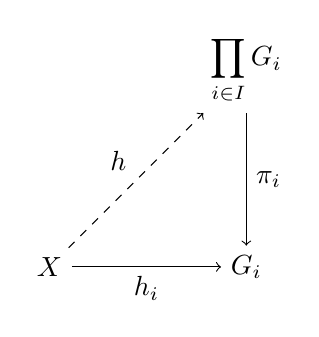
\begin{tikzpicture}[node distance=2.5cm, auto]
	\node (P) {$\displaystyle\prod_{i \in I} \bm{G_i}$};
	\node (Ci) [below of=P] {$\bm{G_i}$};
	\node (X) [left of=Ci] {$\bm{X}$};
	\draw[->] (X) to node [swap] {$h_i$} (Ci);
	\draw[->, dashed] (X) to node {$h$} (P);
	\draw[->] (P) to node {$\pi_i$} (Ci);
\end{tikzpicture}
\end{figure}
\end{prop}
\begin{proof}
Defina a função
	\begin{align*}
	\func{h}{X}{\prod_{i \in I} G_i}{x}{(h_i(x))_{i \in I}}.
	\end{align*}
Da propriedade universal para o produto de conjuntos, $h$ é a única função tal que, para todo $i \in I$, $\pi_i \circ h = h_i$. Basta mostrar que $h$ é homomorfismo de grupos. Por simplicidade, apenas a operação $\opb$ em $G$ será explicitada. Sejam $x_1,x_2 \in X$. Então, como $h_i$ são homomorfismos de grupo,
	\begin{equation*}
	h(x_1x_2) = (h_i(x_1x_2))_{i \in I} = (h_i(x_1)h_i(x_2))_{i \in I} = h(x_1)h(x_2).
	\end{equation*}
\end{proof}

\subsection{Grupo Livre}

\begin{defi}
Seja $C$ um conjunto. O \emph{conjunto de inversos formais} de $C$ é o conjunto $C\inv := C \times \{-1\}$ e seus elementos são denotados $c\inv := (c,-1)$.

Uma \emph{palavra} em $C$ é uma sequência finita $(c_1,\ldots,c_n) \in C^n$. Denota-se $c_1 \cdots c_n$.
\end{defi}

Seja $p=c_1 \cdots c_n$ uma palavra em $C$. A \emph{palavra inversa} de $p$ é a palavra $p\inv := c_n\inv \cdots c_1\inv$.

\begin{defi}
Seja $C$ um conjunto e $p_1,p_2 $ palavras em $C \times \{1,-1\}$. A relação de equivalência entre as palavras $p_1$ e $p_2$ é definida por
	\begin{equation*}
	p_1 \sim p_2 \sse p_1p_2\inv \leadsto e.
	\end{equation*}	
\end{defi}

	\begin{equation*}
	C^* := \bigcup_{n \in \N} (C \times \{1,-1\})^n
	\end{equation*}
 Define-se $C^0 = \{\emptyset\}$.

	\begin{equation*}
	\ger{C} := C^*/\sim
	\end{equation*}
	
	A inclusão é definida.
	\begin{align*}
	\func{\iota}{C}{\ger{C}}{c}{[c]}.
	\end{align*}

\begin{prop}[Propriedade Universal]
Seja $C$ um conjunto, $\bm X = (X,\star)$ um grupo e $f: C \to X$ uma função. Então existe um único homomorfismo de grupos $h: \bm{\ger{C}} \to \bm X$ tal que $h \circ \iota = f$ (o diagrama comuta).
\begin{figure}
\centering
\begin{tikzpicture}[node distance=2.5cm, auto]
	\node (C) {$C$};
	\node (G) [above of=C] {$\displaystyle\bm{\ger{C}}$};
	\node (X) [right of=C] {$\bm X$};
	\draw[->] (C) to node [swap] {$f$} (X);
	\draw[->, dashed] (G) to node {$h$} (X);
	\draw[->] (C) to node {$\iota$} (G);
\end{tikzpicture}
\end{figure}
\end{prop}
\begin{proof}
Defina a função
	\begin{align*}
	\func{h}{\ger{C}}{X}{\left[c_1 \cdots c_n\right] }{f(c_1) \star \cdots \star f(c_n)},
	\end{align*}
de modo que $h([e])=e_X$. Então, para todo $c \in C$,
	\begin{equation*}
	h \circ \iota(c) = h (\iota(c)) = h([c])=f(c).
	\end{equation*}
Logo $h \circ \iota = f$. Para mostrar que é um homomorfismo de grupos, sejam $[c_1 \cdots c_n],$ $[d_1 \cdots d_m] \in \ger{C}$. Então
	\begin{align*}
	h([c_1 \cdots c_n][d_1 \cdots d_m]) &= h([c_1 \cdots c_nd_1 \cdots d_m]) \\
		&= f(c_1) \star \cdots \star f(c_n) \star f(d_1) \star \cdots  \star f(d_m) \\
		&= h([c_1 \cdots c_n]) \star h([d_1 \cdots d_m]).
	\end{align*}
Isso mostra a existência. Para mostrar a unicidade, seja $\overline h: \bm{\ger{C}} \to \bm X$ um homomorfismo de grupos tal que $\overline h \circ \iota = f$. Seja $[c_1 \cdots c_n] \in \ger{C}$. Como $[c_1 \cdots c_n] = [c_1] \cdots [c_n] = \iota(c_1) \cdots \iota(c_n)$, segue que
	\begin{align*}
	\overline h ([c_1 \cdots c_n]) &= \overline h(\iota(c_1) \cdots \iota(c_n)) \\
		&= \overline h(\iota(c_1)) \star \cdots \star \overline h(\iota(c_n)) \\
		&= f(c_1) \star \cdots \star f(c_n) \\
		&= h([c_1 \cdots c_n]),
	\end{align*}
o que implica que $\overline h = h$.
\end{proof}

\subsection{Coproduto de Grupos}

\begin{defi}
Seja $(\bm{G_i})_{i \in I}$ uma família de grupos. O \emph{coproduto} da família $(\bm{G_i})_{i \in I}$ é o par
	\begin{equation*}
	\coprod_{i \in I} \bm{G_i} := \left(G,\opb \right),
	\end{equation*}
em que $G := \ger{\coprod_{i \in I} G_i}$ é o grupo livre sobre o coproduto de conjuntos $\coprod_{i \in I} G_i$ e
	\begin{align*}
	\func{\opb}{G \times G}{G}{([p_1],[p_2])}{[p_1p_2]}.
	\end{align*}
\end{defi}

\begin{prop}[Propriedade Universal]
Sejam $(\bm{G_i})_{i \in I}$ uma família de grupos, $\bm X = (X,\star)$ um grupo e, para todo $i \in I$, $h_i: \bm{G_i} \to \bm X$ um homomorfismo de grupos. Então existe um único homomorfismo de grupos $h: \coprod_{i \in I} \bm{G_i} \to \bm X$ tal que, para todo $i \in I$, $h \circ \iota_i = h_i$ (o diagrama comuta).
\begin{figure}
\centering
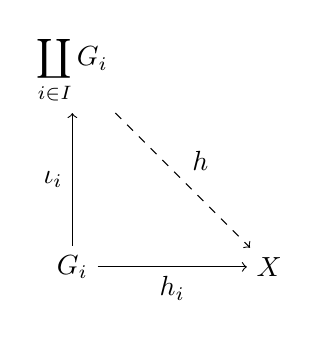
\begin{tikzpicture}[node distance=2.5cm, auto]
	\node (Ci) {$\bm{G_i}$};
	\node (S) [above of=Ci] {$\displaystyle\coprod_{i \in I} \bm{G_i}$};
	\node (X) [right of=Ci] {$\bm X$};
	\draw[->] (Ci) to node [swap] {$h_i$} (X);
	\draw[->, dashed] (S) to node {$h$} (X);
	\draw[->] (Ci) to node {$\iota_i$} (S);
\end{tikzpicture}
\end{figure}
\end{prop}
\begin{proof}
Defina a função
	\begin{align*}
	\func{h}{\ger{\coprod_{i \in I} G_i}}{X}{\left[(g_1,i_1) \cdots (g_n,i_n)\right]}{h_{i_1}(g_1) \star \cdots \star h_{i_n}(g_n)}.
	\end{align*}

Por simplicidade, seja $G := \ger{\coprod_{i \in I} G_i}$. Para mostrar que $h$ é homomorfismo, sejam $[(g_1,i_1) \cdots (g_n,i_n)]$ e $[(g'_1,i'_1) \cdots (g'_m,i'_m)] \in G$. Então
	\begin{align*}
	&h([(g_1,i_1) \cdots (g_n,i_n)][(g'_1,i'_1) \cdots (g'_m,i'_m)]) \\
		&= h([(g_1,i_1) \cdots (g_n,i_n)(g'_1,i'_1) \cdots (g'_m,i'_m)]) \\
		&= h_{i_1}(g_1) \star \cdots \star h_{i_n}(g_n) \star h_{i'_1}(g'_1) \star \cdots \star h_{i'_n}(g'_n) \\
		&= h([(g_1,i_1) \cdots (g_n,i_n)]) \star h([(g'_1,i'_1) \cdots (g'_m,i'_m)]).
	\end{align*}
\end{proof}








































\cleardoublepage
\section{Construções Específicas}

\subsection{Grupo Simples e Subgrupo Normal Maximal}

\begin{defi}
Um \emph{grupo simples} é um grupo não-trivial $\bm G$ cujos únicos subgrupos normais são $\bm{\{e\}}$ e $\bm G$.
\end{defi}

\begin{defi}
Seja $\bm G$ um grupo. Um subgrupo normal \emph{maximal} de $\bm G$ é um subgrupo normal próprio $\bm M \idepro \bm G$ que satisfaz
	\begin{enumerate}
	\item (Maximalidade) Para todo $\bm N \ide \bm G$,
		\begin{equation*}
		M \subseteq N \Rightarrow N = M \ou N = G.
		\end{equation*}
	\end{enumerate}
\end{defi}

\begin{prop}
Sejam $\bm G$ um grupo e $\bm M \ide \bm G$ um subgrupo normal. Então $\bm M$ é maximal se, e somente se, $\bm{G/M}$ é simples.
\end{prop}
\begin{proof} Consideremos a projeção canônica
	\begin{align*}
	\func{\pi}{G}{\quo{G}{M}}{g}{gM}.
	\end{align*}
($\Rightarrow$) Suponhamos que $\bm M$ é maximal. Então $\bm M$ é um subgrupo próprio, o implica que $\bm{G/M}$ é não-trivial. Seja $\bm N \ide \bm{G/M}$. Sabemos que $\bm{\pi^{-1}(N)} \ide \bm G$ (\ref{alge:prop.gru.hominv}). Como $[e] \in N$, então $\pi^{-1}(e) \subseteq \pi^{-1}(N)$. Notando que $\pi^{-1}([e])=\nuc(\pi) = M$, segue que $M \subseteq \pi^{-1}(N)$. Como $\bm M$ é maximal, segue que $\pi^{-1}(N) = N$ ou $\pi^{-1}(N) = G$. Notemos que $N=\pi(\pi^{-1}(N))$, pois $\pi$ é sobrejetiva. No primeiro caso, $N = \pi(\pi^{-1}(N)) = \pi(M) = \{[e]\}$. No segundo caso, $N = \pi(\pi^{-1}(N)) = \pi(G) = G/M$. Portanto $\bm{G/M}$ é simples.

\noindent
($\Leftarrow$) Suponhamos que $\bm{G/M}$ é simples. Seja $\bm N \ide \bm G$ tal que $M \subseteq N$. Como $\pi$ é homomorfismo de grupos sobrejetivo, ssegue que $\pi(N) \ide \bm{G/M}$ (\ref{alge:prop.gru.hom}). Como $\bm{G/M}$ é simples, então $\pi(N) = \{[e]\}$ ou $\pi(N) = G/M$. No primeiro caso, $N = \nuc(\pi) = M$. No segundo caso, $N = \pi^{-1}(\pi(N)) = \pi^{-1}(N) = G$. Logo $\bm M$ é maximal.
\end{proof}

\begin{conj}
Sejam $\bm G$ um grupo e $\bm N \idepro \bm G$ um subgrupo normal próprio. Então $\bm G$ tem subgrupo normal maximal.
\end{conj}
\begin{proof}
Usaremos o lema de Zorn. Seja $P \subseteq \p(G)$ o conjunto de todos os subconjuntos $S \subset G$ tais que $\bm S \idepro \bm G$. Então $(P,\subseteq)$ é um conjunto parcialmente ordenado com a contenção de conjuntos usual. Agora, seja $(C)_{i \in I}$ uma cadeia de $(P,\subseteq)$. Consideremos o conjunto $C := \bigcup_{i \in I} C_i$. Como 

Notemos que $P$ não é vazio, pois $N \in P$. Seja 



Então $P$ tem elemento maximal.
\end{proof}






\subsection{Sequência subnormal}

\begin{defi}
Seja $\bm G$ um grupo. Uma \emph{sequência subnormal} de $\bm G$ é uma sequência finita $(\bm{N_i})_{i \in [n]}$ de subgrupos de $\bm G$ que satisfaz
	\begin{equation*}
	\bm{\{e\}} = \bm{N_0} \ide \cdots \ide \bm{N_{n-1}} = \bm G.
	\end{equation*}
O grupo $\bm{N_{i+1}/N_i}$ é o $i$-ésimo \emph{grupo fator} da sequência.
Uma \emph{sequência normal} é uma sequência subnormal em que, para todo $i \in [n]$, $\bm{N_i} \ide \bm G$.

Uma sequência subnormal \emph{estrita} de $\bm G$ é uma sequência subnormal $(\bm{N_i})_{i \in [n]}$ de $\bm G$ que satisfaz
	\begin{equation*}
	\bm{\{e\}} = \bm{N_0} \idepro \cdots \idepro \bm{N_{n-1}} = \bm G.
	\end{equation*}
	
O comprimento
\end{defi}



\subsection{Conjunto gerador}

\begin{defi}
Seja $\bm G$ um grupo e $S \subseteq G$ um conjunto. O grupo \emph{gerado} por $S$ é o grupo $\bm{\langle S \rangle} \leq \bm G$ em que
	\begin{equation*}
	\langle S \rangle := \set{s_1 \cdots s_n}{n \in \N,\ s_i \in S \ou s_i\inv \in S}.
	\end{equation*}
	\begin{equation*}
	\langle S \rangle := \set{\bigopb_{i \in [n]} s_i}{n \in \N,\ s_i \in S \ou s_i\inv \in S}.
	\end{equation*}
\noindent
Um \emph{conjunto gerador} de $\bm G$ é um conjunto $S \subseteq G$ tal que $\langle S \rangle = G$.
\end{defi}










\subsection{Grupos Simétricos e Alternados}

\begin{defi}
Seja $C$ um conjunto. O \emph{grupo simétrico} de $C$ é o par $\bm{\simm{C}} = (\simm{C},\circ)$, em que	
	\begin{equation*}
	\simm{C} := \set{p: C \to C}{\exists p\inv: C \to C}
	\end{equation*}
é o conjunto de todas as bijeções entre $C$ e $C$, e $\circ$ é a composição de funções. Seja $\alpha$ um número cardinal. Para $C = \alpha$, usa-se a notação $\sime_{\alpha} := \simm{\alpha}$.
\end{defi}

\begin{prop}
	Seja $C$ um conjunto. O grupo simétrico $\bm{\simm{C}}$ é um grupo.
\end{prop}
\begin{proof}
	Se $C=\emptyset$, então $\simm{C}=\{\emptyset\}$. Assim, como $\emptyset \circ \emptyset = \emptyset$, segue que $\circ$ é operação binária em $\{\emptyset\}$. Ainda, segue que $\circ$ é associativa, pois $(\emptyset \circ \emptyset) \circ \emptyset = \emptyset \circ (\emptyset \circ \emptyset)$; tem elemeno neutro $\emptyset$, pois $\emptyset \circ \emptyset = \emptyset$, e que todo elemento tem inverso, pois $\emptyset\inv = \emptyset$.

	Suponhamos, então, que $C \neq \emptyset$ e sejam $p_1,p_2 \in \simm{C}$. Como $p_1$ e $p_2$ são bijeções, a função $p_2 \circ p_1: C \to C$ é uma bijeção entre $C$ e $C$ (\ref{prop:comp.func.inj} e \ref{prop:comp.func.sobr}) e, portanto, $p_2 \circ p_1 \in \simm{C}$. Isso mostra que $\circ$ é uma operação binária em $\simm{C}$. A composição de funções é associativa, pois, para todos $p_1,p_2,p_3 \in \simm{C}$, $p_3 \circ (p_2 \circ p_1) = (p_3 \circ p_2) \circ p_1$ (\ref{prop:comp.func.asso}). Ainda, notemos que $\id_C$ é o elemento neutro de $\bm{\simm{C}}$, pois, para todo $p \in \simm{C}$, vale $p \circ \id_C = \id_C \circ p = p$ (\ref{prop:id.comp.func}). Por fim, como $p$ é uma bijeção, existe função inversa $p\inv: C \to C$ que é bijeção entre $C$ e $C$ (\ref{prop:func.inv.esq} e \ref{prop:func.inv.dir}); logo existe $p\inv \in \simm{C}$ tal que $p \circ p\inv = p\inv \circ p = \id_C$. Portanto concluímos que $\bm{\simm{C}}$ é um grupo.
\end{proof}

\begin{prop}
	Sejam $A$ e $B$ conjuntos tais que $\card{A} = \card{B}$. Então
	\begin{equation*}
	\bm{\simm{A}} \simeq \bm{\simm{B}}.
	\end{equation*}
\end{prop}
\begin{proof}
	Seja $\phi: A \to B$ uma bijeção e considere a função
	\begin{align*}
	\func{h}{\simm{A}}{\simm{B}}{p}{\phi \circ p \circ \phi\inv}.
	\end{align*}
Primeiro notemos que $h$ é homomorfismo de grupos. Sejam $p_1,p_2 \in \simm{A}$. Então
	\begin{align*}
	h(p_2 \circ p_1)(c) &= \phi \circ (p_2 \circ p_1) \circ \phi^{-1} \\
			&= \phi \circ (p_2 \circ \phi\inv \circ \phi \circ p_1) \circ \phi^{-1} \\
			&= (\phi \circ p_2 \circ \phi\inv) \circ (\phi \circ p_1 \circ \phi\inv) \\
			&= h(p_2) \circ h(p_1).
	\end{align*}
Portanto $h$ é um homomorfismo de grupos entre $\bm{\simm{A}}$ e $\bm{\simm{B}}$.

Agora notemos que $h$ é uma bijeção. A inversa de $h$ é a função
	\begin{align*}
	\func{h\inv}{\simm{B}}{\simm{A}}{p}{\phi\inv \circ p \circ \phi},
	\end{align*}
pois, para todo $p \in \simm{B}$,
	\begin{align*}
	(h \circ h\inv) (p) &= h (h\inv(p)) \\
			&= \phi \circ h\inv(p) \circ \phi\inv \\
			&= \phi \circ (\phi\inv \circ p \circ \phi) \circ \phi\inv \\
			&= p \\
			&= \id_{\simm{B}}(p),
	\end{align*}
o que mostra que $h \circ h\inv = \id_{\simm{B}}$, e, para todo $p \in \simm{A}$,
	\begin{align*}
	(h\inv \circ h) (p) &= h\inv (h(p)) \\
			&= \phi\inv \circ h(p) \circ \phi \\
			&= \phi\inv \circ (\phi \circ p \circ \phi\inv) \circ \phi \\
			&= p \\
			&= \id_{\simm{A}}(p),
	\end{align*}
o que mostra que $h\inv \circ h = \id_{\simm{A}}$. Assim, está provado que $h$ é isomorfismo entre $\bm{\simm{A}}$ e $\bm{\simm{B}}$.
\end{proof}

	Essa proposição mostra que podemos estudar somente os grupos simétricos dos números cardinais, pois isso será equivalente a estudar qualquer grupo simétrico. Em particular, para todo conjunto finito, podemos estudar seu grupo simétrico considerando somente o grupo simétrico $\bm\sime_n$, em que $n$ é o número de elementos do conjunto. A partir de agora, as proposições serão considerando esses grupos $\bm\sime_n$.

\begin{prop}
	Seja $n \in \N$. Então $|\sime_n|=n!$.
\end{prop}

\begin{teo}
	Seja $\bm G$ um grupo. Então
	\begin{equation*}
	\bm G \lesssim \bm{\simm{G}}.
	\end{equation*}
\end{teo}
\begin{proof}
	Consideremos a função
	\begin{align*}
	h: G \to \simm{G} & \\
		g \mapsto h(g): & G \to G \\
									&\ x \mapsto g \opb x \\
	\end{align*}
Primeiro, devemos mostrar que $h(g) \in \simm{G}$, para que $h$ esteja bem definida. Para isso, notemos que $h(g)$ está bem definida, já que, para todo $x \in G$, $g \opb x \in G$. Ainda, $h(g)$ é uma bijeção, pois $h(g)\inv = h(g\inv)$, já que, para todo $x \in G$,
	\begin{equation*}
	(h(g) \circ h(g)\inv)(x) = h(g)((h(g)\inv)(x)) = h(g)(g\inv \opb x) = g \opb g\inv \opb x = x = \id_G,
	\end{equation*}
o que mostra que $h(g) \circ h(g)\inv = \id_G$, e
	\begin{equation*}
	(h(g)\inv \circ h(g))(x) = h(g)\inv((h(g)(x)) = h(g)\inv(g \opb x) = g\inv \opb g \opb x = x = \id_G,
	\end{equation*}
o que mostra que $h(g)\inv \circ h(g) = \id_G$. Isso mostra que $h(g)$ é uma bijeção e, portanto, $h(g) \in \simm{G}$.

	Agora, notemos que $h$ é um homomorfismo de grupos, pois, para todos $g_1,g_2 \in G$, segue que, para todo $x \in G$,
	\begin{align*}
	h(g_1 \opb g_2)(x) &= (g_1 \opb g_2) \opb x \\
	&= g_1 \opb (g_2 \opb x) \\
	&= h(g_1)(g_2 \opb x) \\
	&= h(g_1)(h(g_2)(x)) \\
	&= (h(g_1) \circ h(g_2))(x),
	\end{align*}
o que mostra que $h(g_1 \opb g_2) = h(g_1) \circ h(g_2)$. Por fim, notemos que $h$ é injetiva, já que, se $g \in G$ é tal que $h(g)=id_G$, então, para todo $x \in G$,
	\begin{equation*}
	g \opb x = h(g)(x) = \id_G(x) = x,
	\end{equation*}
o que mostra que $g=e_G$ e, portanto, que $\nuc(h)=\{e_G\}$.
\end{proof}

	Esse teorema é um teorema muito importante, pois ele mostra que, de certa forma, todo grupo é um subconjunto de permutações. Por causa disso que grupos são pensados como os objetos algébricos que modelam a simetria.

\subsubsection{Permutações e Órbitas}

\begin{defi} Seja $n \in \N$. Uma \emph{permutação} de $n$ objetos é um elemento $p \in \sime_n$, denotado por
	\begin{equation*}
	p = \begin{pmatrix}
				1 & 2 & \cdots & n-1 & n \\
				p(1) & p(2) & \cdots &  p(n-1)  & p(n)
			\end{pmatrix}.
	\end{equation*}
\end{defi}

\begin{nota}
	Seja $n \in \N$. A composição de duas permutações $p_1,p_2 \in \sime_n$, quando representadas na notação acima, é denotada
	\begin{equation*}
	p_2 \circ p_1 = \bigl(\begin{smallmatrix}
				1 & 2 & \cdots & n-1 & n \\
				p_2(1) & p_2(2) & \cdots &  p_2(n-1)  & p_2(n)
			\end{smallmatrix}\bigr)
			\bigl(\begin{smallmatrix}
				1 & 2 & \cdots & n-1 & n \\
				p_1(1) & p_1(2) & \cdots &  p_1(n-1)  & p_1(n)
			\end{smallmatrix}\bigr).
	\end{equation*}
\end{nota}

\begin{defi}
	Sejam $n \in \N$ e $p \in \sime_n$. A \emph{matriz de permutação} de $p$ é a matriz $[p] \in \M_n (\Z)$ cujas entradas são dadas por
	\begin{equation*}
		[p]_{i,j} = \delta_{i,p(j)} = \begin{cases}
												1 & i=p(j) \\
												0 & i \neq p(j).
												\end{cases}
	\end{equation*}
	O \emph{conjunto das matrizes de permutação} de $\sime_n$ é o conjunto
	\begin{equation*}
		[\sime_n] := \set{[p]}{p \in \sime_n}.
	\end{equation*}
\end{defi}

\begin{prop}
	Seja $n \in \N$. Então o par $\bm{[\sime_n]}=([\sime_n],\cdot)$, em que $\cdot$ é o produto de matrizes, é um grupo, e
	\begin{equation*}
	\bm{\sime_n} \simeq \bm{[\sime_n]}.
	\end{equation*}
\end{prop}
\begin{proof}
	Primeiro, notemos que, para todos $p,q \in \sime_n$,
	\begin{equation*}
	[p][q]_{i,j} = \sum_{k=0}^{n-1} [p]_{i,k}[q]_{k,j} = \sum_{k=0}^{n-1} \delta_{i,p(k)}\delta_{k,p(j)}.
	\end{equation*}
	Mas o produto $\delta_{i,p(k)}\delta_{k,p(j)}$ é igual a 1 se, e somente se, $i=p(k)$ e $k=q(j)$. Como $p$ é bijeção, a segunda consição é equivalente a $p(k)=pq(j)$, e isso mostra que as duas consições são equivalentes a $i=p(k)=pq(j)$. Como $p$ é bijeção, para cada $i \in [n]$, $k=p\inv(i)$ é o único $k \in [n]$ tal que a condição é satisfeita, e segue que
	\begin{equation*}
	[p][q]_{i,j} = \sum_{k=1}^n \delta_{i,p(k)}\delta_{k,p(j)} = \sum_{k=1}^n \delta_{i,pq(j)} = [pq]_{i,j}.
	\end{equation*}
e, como $pq \in \sime_n$, então $[p][q]=[pq] \in [\sime_n]$. Isso mostra que o produto de matrizes é uma operação binária em $[\sime_n]$. Agora, disso segue que $[p][p\inv]=[pp\inv]=[id]$

%MOSTRAR QUE O INVERSO DE P ESTA NO GRUPO




Disso, segue que $\bm{[\sime_n]}$ é um grupo, pois é subgrupo de $\M_n(\Z)$. Por fim, consideremos a função
	\begin{align*}
	\func{h}{\sime_n}{[\sime_n]}{p}{[p]}.
	\end{align*}
Note que que $h$ é homomorfismo, pois, para todos $p,q \in \sime_n$,
	\begin{equation*}
	h(pq) = [pq]= [p][q] = h(p)h(q).
	\end{equation*}
Ainda, $h$
\end{proof}

\begin{defi}
	Sejam $n \in \N$, $p \in \sime_n$ e $m \in [n]$. A \emph{órbita de $m$ sob $p$} é o conjunto
	\begin{equation*}
	\orb_p(m) := \set{p^k(m)}{k \in \Z}.
	\end{equation*}
O \emph{período} da órbita $\orb_p(m)$ é o número $\card{\orb_p(m)}$. Uma \emph{órbita trivial} é uma órbita de período $1$. Uma órbita de $p$ é a órbita de um elemento $m \in [n]$ sob $p$.

	O \emph{conjunto de órbitas} de $p$ é o conjunto
	\begin{equation*}
	\orb_p := \set{\orb_p(m)}{m \in [n]}.
	\end{equation*}
\end{defi}

\begin{prop}
	Sejam $n \in \N$ e $p \in \sime_n$. O conjunto $\orb_p$ é uma partição de $[n]$.
\end{prop}
\begin{proof}
	Primeiro, notemos que $m \in \orb_p(m)$ e, portanto, $\emptyset \nsubseteq \orb_p$. Ainda, $\bigcup_{m \in [n]} \orb_p(m) = [n]$, já que, para todo $m \in [n]$, $m \in \orb_p(m)$, o que mostra que $[n] \subseteq \bigcup_{m \in [n]}$ e, para todo $l \in \bigcup_{m \in [n]} \orb_p(m)$, existe $m \in [n]$ tal que $l \in \orb_p(m)$ e, portanto, existe $k \in \N$ tal que $l=p^k(m) \in [n]$, o que mostra que $\bigcup_{m \in [n]} \subseteq [n]$. Por fim, sejam $o_1,o_2 \in \orb_p$. Então existem $m_1,m_2 \in [n]$ tais que $o_1=\orb_p(m_1)$ e $o_2=\orb_p(m_2)$. Se existe $l \in \orb_p(m_1) \cap \orb_p(m_2)$, então existem $k_1,k_2 \in \Z$ tais que $l=p^{k_1}(m_1)=p^{k_2}(m_2)$. Assim, segue que $m_1=p^{k_2-k_1}(m_2)$ e, portanto, $m_1 \in \orb_p(m_2)$. Mas isso implica que $\orb_p(m_1) \subseteq \orb_p(m_2)$; a inclusão contrária é análoga e concluímos que $\orb_p(m_1) = \orb_p(m_2)$. Logo $\orb_p$ é uma partição de $[n]$.
\end{proof}

\subsubsection{Permutações, Ciclos e Transposições}

\begin{defi}
	Sejam $n,k \in \N$. Um \emph{ciclo} de $\sime_n$ é um elemento $c \in \sime_n$ para o qual existe $m \in [n]$ tal que, para todo $m' \in [n]$, $c(m')=m'$ ou existe $d \in [n]$ tal que $m'=c^d(m)$. O \emph{comprimento} de um ciclo é a ordem desse ciclo. Um ciclo $c$ cujo comprimento é $k$ é denotado
	\begin{equation*}
	c = \bigl(m \ c(m) \ c^2(m) \ \cdots \  c^{k-2}(m) \ c^{k-1}(m)\bigr).
	\end{equation*}
\end{defi}


\begin{prop}
	Sejam $n \in \N$.
	\begin{enumerate}
	\item Se $c_1,c_2 \in \sime_n$ são ciclos disjuntos, então $c_2 \circ c_1 = c_1 \circ c_2$.
	\end{enumerate}
\end{prop}

\begin{prop}[Fatoração de Permutação]
	Seja $n \in \N$ e $p \in \sime_n$. Então existem únicos ciclos $c_1,\ldots,c_k \in \sime_n$ disjuntos dois a dois tais que $p=c_1 \circ \cdots \circ c_k$.
\end{prop}
\begin{proof}
	Seja $k := \card{\orb_p}$. O cojunto $\orb_p$ particiona $[n]$. Sejam $(o_k)_{i \in [k]}$ uma indexação de $\orb_p$ e $m_1,\cdot,m_k \in [n]$ tais que $o_i=\orb_p(m_i)$ para todo $i \in [k]$, e seja $k_i := \card{\orb_p(m_i)}$. Definamos $c_i :=  \bigl( m_i \ \cdots \  p^{k_i-1}(m_i)\bigr)$. Então segue que
	\begin{equation*}
	p = \bigtimes_{i=1}^k \bigl( m_i \ \cdots \  p^{k_i-1}(m_i)\bigr) = \bigtimes_{i=1}^k c_i.
	\end{equation*}
\end{proof}



\subsection{Grupos Cíclicos}

\subsection{Grupos Diedrais}


\cleardoublepage
\section{Ação de Grupos}

A noção de uma ação de grupo, de certa forma, generaliza uma estratégia usada na demonstração do teorema de que todo grupo é isomorfo a um subgrupo de seu grupo simétrico.

\begin{defi}
Sejam $\bm G$ um grupo e $X$ um conjunto. Uma \emph{ação} de $\bm G$ em $X$ é um homomorfismo de grupos
%	\begin{equation*}
%	A: \bm G  \to \bm{\simm{X}}.
%	\end{equation*}
	\begin{align*}
	\func{A}{G}{\simm{X}}{g}{
		\begin{aligned}[t]
		\func{g\pt}{X}{X}{x}{g\pt x.}
		\end{aligned}
	}
	\end{align*}
Denota-se $A\colon \bm G \age X$. Diz-se que o grupo $\bm G$ \emph{age} no conjunto $X$, e denota-se $\bm G \age X$, se, e somente se, existe ação de $\bm G$ em $X$.
%O grupo $\bm G$ é o \emph{grupo de funções} e o conjunto $X$ é um \emph{$\bm G$-conjunto}.
\end{defi}

A definição acima é uma definição muito simplificada pois ela depende de conceitos um pouco mais complexos, como de homomorfismo de grupos e de grupo simétrico. A proposição abaixo mostra como essa definição é equivalente a uma definição mais explícita de ação de grupo que também é comumente usada.

\begin{prop}
Sejam $X$ um conjunto e $\bm G$ um grupo. Então $\bm G \age X$ se, e somente se, existe uma função
	\begin{align*}
	\func{\pt}{G \times X}{X}{(g,x)}{g\pt x}
	\end{align*}
que satisfaz
\begin{enumerate}
\item (Identidade) Para todo $x \in X$,
	\begin{equation*}
	e \pt x = x;
	\end{equation*}
\item (Compatibilidade) Para todos $g_0,g_1 \in G$ e $x \in X$,
	\begin{equation*}
	(g_1g_0) \pt x = g_1 \pt (g_0 \pt x).
	\end{equation*}
\end{enumerate}
\end{prop}
\begin{proof}
Se existe ação $A: \bm G \age X$, basta definir $g \pt x := A(g)(x)$ e segue que $e\pt = \id$ e $(g_1g_0) \pt = g_1 \pt \circ g_0 \pt$. Reciprocamente, definimos a ação $A$ a partir de $\pt$ da mesma forma e, se $g_0,g_1 \in G$ e $x \in X$, segue que
	\begin{equation*}
	A(g_1g_0)(x) =(g_1g_0) \pt x = g_1 \pt (g_0 \pt x) = A(g_1)(A(g_0)(x)) = A(g_1) \circ A(g_0)(x),
	\end{equation*}
logo $A(g_1g_0)=A(g_1) \circ A(g_0)$.
\end{proof}

Essa proposição é geralmente considerada a definição de uma ação \emph{à esquerda} de $\bm G$ em $X$ por causa da posição em que a composição ocorre. Analogamente, uma ação à direita pode ser definida, mas toda ação à direita pode ser traduzida em uma ação à esquerda, de modo que é suficiente estudar somente ações à esquerda. É comum, ainda, estudar ações em conjuntos $X$ com alguma estrutura adicional, geralmente uma topologia. Nesse caso, exige-se que a ação seja uma função contínua, mas também é necessário que $G$ tenha uma estrutura topológica, portanto isso não será definido com cuidado agora.

\subsection{Órbitas e Estabilizadores}

\begin{defi}
Sejam $X$ um conjunto, $\bm G$ um grupo, $\bm G \age X$ e $x \in X$. A \emph{órbita} de $x$ sob $\bm G$ é o conjunto
	\begin{equation*}
	G \pt x := \set{g\pt x}{g \in G}.
	\end{equation*}
\end{defi}

\begin{defi}
Sejam $X$ um conjunto, $\bm G$ um grupo, $A: \bm G \age X$ e $x \in X$. O \emph{estabilizador} de $x$ é
	\begin{equation*}
	G_x = \set{g \in G}{g\pt x = x} = A\inv(\{\id\}) = \nuc(A).
	\end{equation*}
\end{defi}

O estabilizador de $x$ é um grupo e por isso é chamado de \emph{subgrupo estabilizador} de $\bm G$ com respeito a $x$, e também é conhecido como \emph{grupo de isotropia} de $x$.

\section{Grupo Linear Geral}

\begin{defi}
Sejam $\bm C$ um corpo e $n \in \N$. O \emph{grupo linear geral} de $\bm C$ de ordem $n$ é o conjunto
	\begin{equation*}
	\GL_n(\bm C) := \set{M \in \M_{n\times n}(\bm C)}{\det M \neq 0}.
	\end{equation*}
Se $\bm V$ é um espaço vetorial finito de dimensão $d$ sobre um corpo $\bm C$, o \emph{grupo linear geral} de $\bm V$ é
	\begin{equation*}
	\GL(\bm V) := \GL_n(\bm C).
	\end{equation*}
\end{defi}

Como $\det(AB) = \det(A)\det(B)$ e as matrizes invertíveis são as que têm determinante não nulo, segue que o conjunto acima forma um grupo com respeito ao produto de matrizes.

\begin{defi}
Sejam $\bm C$ um corpo e $n \in \N$. O \emph{grupo linear especial} de $\bm C$ de ordem $n$ é o conjunto
	\begin{equation*}
	\SL_n(\bm C) := \set{M \in \GL(n,\bm C)}{\det M =1}.
	\end{equation*}
\end{defi}


\section{Representação de Grupos}

\begin{defi}
Sejam $\bm G$ um grupo e $\bm V$ um espaço vetorial sobre um corpo $\bm C$. Uma \emph{representação} de $\bm G$ em $\bm V$ é um homomorfismo de grupos
	\begin{equation*}
	\rho: \bm G \to \GL(\bm V).
	\end{equation*}
O espaço $\bm V$ é o \emph{espaço de representação} e a dimensão de $\bm V$ é a \emph{dimensão da representação}.
\end{defi}

\begin{defi}
Seja $\bm V$ um espaço vetorial sobre um corpo $\bm C$.
\end{defi}








\cleardoublepage
\chapter{Anéis}

\section{Construções Algébricas}

\subsection{Anel e Subanel}

\begin{defi}
Um \emph{anel} é uma lista $\bm A=(A,+,-,0,\times,1)$ tal que
	\begin{enumerate}
	\item $(A,+,-,0)$ é um grupo comutativo, em que $+$ é a \emph{adição}, $-$ é a \emph{subtração} e $0$ é a \emph{nulidade} (ou o \emph{zero}) de $\bm A$;
	\item $(A,\times,1)$ é um monoide comutativo, em que $\times$ é a \emph{multiplicação} e $1$ é a \emph{unidade} (ou o \emph{um}) de $\bm A$;
	\item A multiplicação $\times$ é distributiva sobre a adição $+$.
	\end{enumerate}
% A imagem de dois elementos $a_1,a_2 \in A$ pela adição é chamada de \emph{soma} de $a_1$ e $a_2$ e denotada por $a_1+a_2$. A imagem de $a_1,a_2$ pela multiplicação é chamada de \emph{produto} de $a_1$ e $a_2$ e denotada por $a_1 \cdot a_1$ ou $a_1a_2$.
\end{defi}

%\begin{defi}
%	Um \emph{anel} é uma tripla $\bm A=(A,+,\cdot)$ em que
%	\begin{enumerate}
%	\item $(A,+)$ é um grupo comutativo com elemento neutro chamado de \emph{zero} ou \emph{nulidade} e representado por $0$ (ou $0_A$, caso exista ambiguidade).
%	\item $(A,\cdot)$ é um monoide comutativo com elemento neutro chamado de \emph{um} ou \emph{unidade} e representado por $1$ (ou $1_A$, caso exista ambiguidade).
%	\item A operação $\cdot$ é distributiva sobre $+$.
%	\end{enumerate}
%As operações $+$ e $\cdot$ são chamadas, respectivamente, de \emph{adição} e \emph{multiplicação}. A imagem de dois elementos $a_1,a_2 \in A$ pela adição é chamada de \emph{soma} de $a_1$ e $a_2$ e denotada por $a_1+a_2$. A imagem de $a_1,a_2$ pela multiplicação é chamada de \emph{produto} de $a_1$ e $a_2$ e denotada por $a_1 \cdot a_1$ ou $a_1a_2$.
%\end{defi}
\begin{nota}
O símbolo de multiplicação $\times$ será suprimido sempre que possível, de modo que denotaremos $a_0a_1$ para $a_0 \times a_1$, e notação da multiplicação terá preferência sobre a da adição e a da substração, pois $\times$ é distributiva sobre $+$, de modo que denotaremos $a_0a_1 + a_2$ para $(a_1a_2) + a_3$ e $-a_1a_2$ para $-(a_1a_2)$. Os símbolos operatórios relativos à adição e à multiplicação serão, respectivamente,
	\begin{equation*}
	\sum \e \bigtimes.
	\end{equation*}
O elemento $a$ multiplicado por si mesmo $n$ vezes será denotado $a^n$. Denotaremos o inverso de um elemento $a \in A$ sob $\times$ por $a\inv$, se ele existir, pois sabemos que é único (\ref{prop:unic.inv}).
\end{nota}

%\begin{nota}
%Como $(A,+)$ é um grupo, denotaremos o inverso de um elemento $a \in A$ sob $+$ por $-a$, e escreveremos $a_1 - a_2$ para $a_1 + (-a_2)$. Ainda, a multiplicação tem preferência na notação; ou seja, $a_1a_2+a_3 = (a_1 \cdot a_2)+a_3$ e $-a_1a_2 = -(a_1 \cdot a_2)$. Denotaremos o inverso de um elemento $a \in A$ sob $\cdot$ por $a^{-1}$, se ele existir, pois sabemos que é único (\ref{prop:unic.inv}). Os símbolos operatórios relativos à adição e à multiplicação serão, respectivamente, $\sum$ e $\bigtimes$. Caso não haja ambiguidade, denotaremos um anel pelo símbolo que denota seu conjunto escrito em negrito, como em $\bm A=(A,+,\cdot)$.
%\end{nota}

Um comentário sobre as identidades $0$ e $1$. Se $0=1$, o anel será \emph{trivial}, no sentido de que $0$ será seu único elemento, mas mantemos esse caso na definição pois, mais à frente, quando estudarmos anéis quocientes, será proveitoso que qualquer anel quociente seja um anel, e se quocientarmos um anel por ele mesmo, temos o anel trivial.

\begin{prop}
Seja $\bm A$ um anel. Então, para todos $a,a' \in A$,
	\begin{enumerate}
	\item $0a = 0$;
	\item Se $0=1$, então $A=\{0\}$;
	\item $-(aa') = (-a)a'$.
	\end{enumerate}
\end{prop}
\begin{proof}
	\begin{enumerate}
	\item
%		\begin{align*}
%		0 \cdot a &= 0 \cdot a + 0 \\
%			&= 0 \cdot a + (0 \cdot a - 0 \cdot a) \\
%			&= (0 \cdot a + 0 \cdot a) - 0 \cdot a \\
%			&= (0+0) \cdot a - 0 \cdot a \\
%			&= 0 \cdot a - 0 \cdot a \\
%			&= 0.
%		\end{align*}
		\begin{align*}
		0 a &= 0 a + 0 \\
			&= 0 a + (0 a - 0 a) \\
			&= (0 a + 0 a) - 0 a \\
			&= (0+0) a - 0 a \\
			&= 0 a - 0 a \\
			&= 0.
		\end{align*}
	
	\item Se $0=1$, então, para todo $a \in A$,
		\begin{equation*}
		a = 1a = 0a = 0;
		\end{equation*}	
	
	\item
%		\begin{align*}
%		-(a \cdot b) &= -(a \cdot b) + 0 \\
%			&= -(a \cdot b) + 0 \cdot b \\
%			&= -(a \cdot b) + (a - a) \cdot b \\
%			&= -(a \cdot b) + (a \cdot b + (-a) \cdot b) \\
%			&= (-(a \cdot b) + a \cdot b) + (-a) \cdot b \\
%			&= 0 + (-a) \cdot b \\
%			&= (-a) \cdot b.
%		\end{align*}
		\begin{align*}
		-(a a') &= -(a a') + 0 \\
			&= -(a a') + 0 a' \\
			&= -(a a') + (a - a) a' \\
			&= -(a a') + (a a' + (-a) a') \\
			&= (-(a a') + a a') + (-a) a' \\
			&= 0 + (-a) a' \\
			&= (-a) a'.
		\end{align*}
	\end{enumerate}
\end{proof}

\begin{defi}
Seja $\bm A$ um anel. O conjunto dos elementos invertíveis sob multiplicação de $\bm A$ é denotado por $A^*$.
\end{defi}

\begin{prop}
Seja $\bm A$ um anel. O par $(A^*,\times|_{(A^*)^2},\inv,1)$ é um grupo comutativo.
\end{prop}
\begin{proof}
A tripla $(A,\times,1)$ é um monoide comutativo com identidade $1$. Portanto segue que a quádrupla $(A^*,\times|_{(A^*)^2},\inv,1)$ é um grupo (em que $a\inv$ denota o inverso de $a$ sob $\times$). Como $\times$ é comutativa, então $(A^*,\times|_{(A^*)^2},\inv,1)$ também o é.
\end{proof}

\begin{defi}
Seja $\bm A=(A,+,-,0,\times,1)$ um anel. Um \emph{subanel} de $\bm A$ é um anel $\bm S=(S,+_S,\times_S)$ em que $S \subseteq A$, $+_S = +|_{S \times S}$ e $\times_S = \times|_{S \times S}$. Denota-se $\bm S \leq \bm A$. Um subanel \emph{próprio} de $\bm A$ é um subanel $\bm S \leq \bm A$ em que $S$ é um conjunto próprio de $A$ ($S \subset A$). Denota-se $\bm S < \bm A$.
\end{defi}

\begin{prop}
Sejam $\bm A=(A,+,\times)$ um anel e $S \subseteq A$. Então
	\begin{equation*}
	\bm S=(S,+|_{S \times S},\times|_{S \times S})
	\end{equation*}
é um anel com $1 \in S$ se, e somente se,
	\begin{enumerate}
	\item $(S,+|_{S \times S})$ é um subgrupo comutativo de $(A,+)$:
			\begin{enumerate}
			\item (Não-vacuidade) $S \neq \emptyset$;
			\item (Fechamento) $\forall s_1,s_2 \in S \qquad s_1 + s_2 \in S$;
			\item (Invertibilidade) $\forall s \in S \qquad -s \in S$;
			\end{enumerate}
	\item $(S,\times|_{S \times S})$ é um submonoide comutativo de $(A,\times)$ com $1 \in S$:
			\begin{enumerate}
			\item (Identidade) $1 \in S$;
			\item (Fechamento) $\forall s_1,s_2 \in S \qquad s_1 \times s_2 \in S$.
			\end{enumerate}
	\end{enumerate}
\end{prop}
\begin{proof}
($\Rightarrow$) Suponhamos que $\bm S$ é um anel com $1 \in S$.
(Subgrupo) Como $S \subseteq A$ e $(S,+|_{S \times S})$ um grupo comutativo, então é um subgrupo de $(A,+)$ por definição de subgrupo (o que é equivalente às propriedades listadas) e é comutativo (\ref{alge:prop.subgru})).
(Subanel)  Como $S \subseteq A$ e $(S,\times|_{S \times S})$ um monoide comutativo com $1 \in S$, então é um submonoide de $(A,\times)$ por definição de submonoide (o que é equivalente às propriedades listadas) e é comutativo (\ref{alge:prop.submon}).

($\Leftarrow$) Suponhamos, agora, que $(S,+|_{S \times S})$ é subgrupo comutativo de $(A,+)$ e $(S,\times_{S \times S})$ é submonoide comutativo de $(A,\times)$.
(Grupo comutativo) Como $(S,+|_{S \times S})$ é subgrupo comutativo, então é um grupo comutativo por definição de subgrupo. (Monoide comutativo) Como $(S,\times|_{S \times S})$ é submonoide comutativo, então é um monoide comutativo por definição de monoide. (Distributividade) Sejam $s_1,s_2,s_3 \in S$. Então
	\begin{align*}
	s_1 \times|_{S \times S} (s_2 +|_{S \times S} s_3) &= s_1 \times (s_2 + s_3) \\
		&= (s_1 \times s_2) + (s_1 \times s_3) \\
		&= (s_1 \times| _{S \times S} s_2) +|_{S \times S} (s_1 \times|_{S \times S} s_3).
	\end{align*}
Logo $\times_{S \times S}$ é distributiva sobre $+ \times_{S \times S}$.
\end{proof}

\subsection{Ideais e Anéis Quocientes}

\begin{defi}
	Seja $\bm A$ um anel. Um \emph{ideal} de $\bm A$ é um conjunto não vazio $I \subseteq A$ tal que
	\begin{enumerate}
	\item $\forall i_1,i_2 \in I \qquad i_1 - i_2 \in I$
	\item $\forall a \in A, i \in I \qquad ai \in I$
	\end{enumerate}
Denotamos que $I$ é ideal de $\bm A$ por $I \ide A$. Ainda, $I \idepro A$ significa que $I \neq A$ e $I \ide A$.
\end{defi}

	É interessante observar que $I$ é subgrupo de $(A,+)$. A definição de ideal difere da definição de subanel na propriedade 2.

\begin{prop}
	Sejam $\bm A$ um anel e $I \ide A$. Então
	\begin{enumerate}
	\item $0 \in I$;
	\item $\forall i_1,i_2 \in I \qquad i_1 + i_2 \in I$;
	\item $1 \in I \Rightarrow I=A$;
	\item $\{0\}$ e $A$ são ideais de $A$.
	\end{enumerate}
\end{prop}
\begin{proof}
	\begin{enumerate}
	\item Seja $i \in I$. Então $0 = i-i \in I$.
	\item Sejam $i_1,i_2 \in I$. Pelo item anterior, sabemos que $0 \in I$, o que implica $-i_2 = 0 - i_2 \in I$. Logo $i_1 + i_2 = i_1 - (-i_2) \in I$.
	\item Se $1 \in I \ide A$, então, para todo $a \in A$, temos $a=a\cdot1 \in A$. Logo $I=A$.
	\item Consideremos $\{0\}$. Se $i \in \{0\}$, então $i=0$. Portanto, para todo $a \in A$ e $i \in \{0\}$, temos $i-i=0 \in \{0\}$ e $ai=0 \in \{0\}$. Logo $\{0\} \ide A$. Agora, consideremos $A$. Para todo $a_1,a_2 \in A$, temos $a_1-a_2 \in A$ e $a_1a_2 \in A$. Logo $A \ide A$.
	\end{enumerate}
\end{proof}

\begin{prop}
	Sejam $\bm A$ um anel e $(I_j)_{j \in J}$ uma família de ideais de $\bm A$. Então
	\begin{equation*}
	I := \bigcap_{j \in J} I_j
	\end{equation*}
é um ideal de $\bm A$.
\end{prop}
\begin{proof}
	Sejam $i_1,i_2 \in I$ e $a \in A$. Então, para todo $j \in J$, $i_1,i_2 \in I_j$ e, como $I_j$ é ideal de $\bm A$, segue que $i_1-i_2 \in I_j$ e que $ai_1 \in W_i$. Logo $i_1-i_2 \in I$ e $ai_1 \in I$, o que mostra que $I$ é ideal de $\bm A$.
\end{proof}

\begin{prop}
	Sejam $\bm A$ um anel e $(I_j)_{n \in \N}$ uma sequência crescente de ideais de $\bm A$; ou seja, $I_1 \subseteq I_2 \subseteq \cdots \subseteq I_n \subseteq \cdots$. Então
	\begin{equation*}
	I := \bigcup_{n \in \N} W_n
	\end{equation*}
é um ideal de $\bm A$.
\end{prop}
\begin{proof}
	Sejam $i_1,i_2 \in I$. Então existem $n,m \in \N$ tais que $i_1 \in I_n$ e $i_2 \in I_m$. Nesse caso, $I_n \subseteq I_m$ ou $I_m \subseteq I_n$. Sem perda de generalidade, suponhamos o primeiro caso. Então segue que $i_1 \in I_m$ e, portanto, $i_1-i_2 \in I_m$, o que mostra que $i_1-i_2 \in I$. Agora, seja $a \in A$ e notemos que, como $I_n$ é ideal de $\bm A$, segue qque $ai_1 \in I_n$. Logo $ai_1 \in I$, o que mostra que $I$ é ideal de $\bm A$.
\end{proof}


\begin{defi}
	Sejam $\bm A$ um anel e $a_1,\ldots,a_n \in A$. Definimos o conjunto
	\begin{equation*}
	\sum_{i=1}^n a_iA = a_1A + \ldots + a_nA := \set{\sum_{i=1}^n a_ib_i}{b_i \in A}.
	\end{equation*}
\end{defi}

\begin{prop}
	Sejam $\bm A$ um anel e $a_1,\ldots,a_n \in A$. Então
	\begin{equation*}
	I := \sum_{k=1}^n a_kA \ide A.
	\end{equation*}
\end{prop}
\begin{proof}
	Sejam $a \in A$ e $i_1,i_2 \in I$ tais que $i_1=\sum_{k=1}^n a_ib_i$ e $i_2=\sum_{k=1}^n a_ic_i$. Então
	\begin{equation*}
	i_1-i_2=\sum_{k=1}^n a_kb_k - \sum_{k=1}^n a_kc_k = \sum_{k=1}^n a_k(b_k-c_k) \in I,
	\end{equation*}
pois $(b_k-c_k) \in A$ para todo $k \in \{1,\ldots,n\}$. Ainda,
	\begin{equation*}
	ak_1=a\sum_{k=1}^n a_kb_k= \sum_{k=1}^n a_k(ab_k) \in I,
	\end{equation*}
pois $ab_k \in A$ para todo $k \in \{1,\ldots,n\}$. Logo $I \ide A$.
\end{proof}

	Esse ideal é chamado de ideal de $A$ gerado por $a_1,\ldots,a_n$.

\begin{defi}
	Seja $\bm A$ um anel. Um \emph{ideal principal} de $\bm A$ é um ideal $I \ide A$ tal que
	\begin{enumerate}
	\item $\exists a \in A \qquad I=aA$.
	\end{enumerate}
\end{defi}

\begin{prop}
\label{pro:corp.sse.ide}
	Seja $\bm A$ um anel. Então $\bm A$ é um corpo se, e somente se, $\bm A$ é um anel não-trivial cujos únicos ideais de $\bm A$ são $\{0\}$ e $A$.
\end{prop}
\begin{proof}
	Suponha que $\bm A$ é um corpo. Então $(A\setminus\{0\},\cdot)$ é um grupo e, portanto, $A \neq \emptyset$. Seja $I \ide A$ e suponha que $I \neq \{0\}$. Então existe $i \in I\setminus\{0\}$. Como $\bm A$ é corpo, existe $i^{-1} \in A$. Portanto $1=i^{-1}i \in I$. Logo $I=A$.

	Por outro lado, suponha que os únicos ideais de $A$ são $\{0\}$ e $A$. Como $\bm A$ é não-trivial, seja $a \in A\setminus\{0\}$ e consideremos o ideal $I=aA$. Notemos que $a=a \cdot 1 \in aA$, o que implica $I \neq \{0\}$. Portanto $I=A$. Mas então $1 \in aA$, o que significa que deve existir $b \in A$ tal que $1=ab$; ou seja, todo $a \in A\setminus\{0\}$ tem inverso em $A$. Logo $\bm A$ é corpo.
\end{proof}

\begin{prop}
	Sejam $\bm A$ um anel e $I \ide A$. A relação binária $\sim_I$ em $A$, definida por
	\begin{equation*}
	a \sim_I b \Leftrightarrow a-b \in I,
	\end{equation*}
é uma relação de equivalência.
\end{prop}
\begin{proof} Vamos demonstrar as três propriedades de uma relação de equivalência.
	\begin{enumerate}
	\item (Reflexividade) Seja $a \in A$. Então $a-a=0 \in I$. Logo $a \sim_I a$.
	\item (Simetria) Sejam $a_1,a_2 \in A$ tais que $a_1 \sim_I a_2$. Então $(a_1-a_2) \in I$. Mas $0 \in I$, o que implica $a_2-a_1 = 0-(a_1-a_2) \in I$. Logo $a_2 \sim_I a_1$.
	\item (Transitividade) Sejam $a_1,a_2,a_3 \in A$ tais que $a_1 \sim_I a_2$ e $a_2 \sim_I a_3$. Então $(a_1-a_2),(a_2-a_3) \in I$, o que implica $a_1-a_3=(a_1-a_2)+(a_2-a_3) \in I$. Logo $a_1 \sim_I a_3$.
	\end{enumerate}
\end{proof}

\begin{defi}
	Sejam $\bm A$ um anel e $I \ide A$. O conjunto $a+I := \{a+i : i \in I\}$ é a \emph{classe lateral} de $I$ com representante $a$. O conjunto das classes laterais de $A$ é denotado por $A/I := \{a+I : a \in A\}$.
\end{defi}

\begin{prop}
	Sejam $(A,+,\cdot)$ um anel, $I \ide A$ e $\sim_I$ a relação de equivalência definida na proposição anterior e $a \in A$. Então a classe de equivalência $[a]=\{b \in A : b \sim_I a\}$ é igual à classe lateral $a+I$ e, por consequência, o conjunto quociente $A/\sim_I$ é igual ao conjunto $A/I$.
\end{prop}
\begin{proof}
	Seja $b \in [a]$. Então $b-a \in I$; ou seja, existe $i \in I$ tal que $b-a=i$. Mas isso implica $b=a+i$, que implica, por sua vez, que $b \in a+I$. Por outro lado, seja $b \in a+I$. Então existe $i \in I$ tal que $b=a+i$; ou seja, $b-a=i$, que implica $b-a \in I$ e, assim, $b \in [a]$. Disso, vem que $A/\sim_I = A/I$.
\end{proof}

	Uma consequência disso é que o conjunto $A$ é particionado em classes laterais de $I$. Outra consequência é que duas classes laterais são iguais se, e somente se, a diferença entre seus representantes está em $I$.

\begin{defi}
	Sejam $\bm A$ um anel, $I \ide A$ e $a_1,a_2 \in A$. Então definimos as operações binárias $\oplus$ e $\odot$ em $A/I$ por
	\begin{equation*}
	(a_1+I) \oplus (a_2+I) := (a_1+a_2)+I \qquad \qquad (a_1+I) \odot (a_2+I) := (a_1 \cdot a_2)+I
	\end{equation*}
Denotaremos $\oplus$ e $\odot$ por $+$ e $\cdot$ quando não existir ambiguidade.
\end{defi}

\begin{prop}
	As operações $\oplus$ e $\odot$ da definição anterior estão bem definidas.
\end{prop}
\begin{proof}
	Sejam $a_1,a_2,b_1,b_2 \in A$ tais que $a_1+I=a_2+I$ e $b_1+I=b_2+I$. Primeiro, vamos mostrar que $\oplus$ está bem definida. Devemos mostrar que $(a_1+b_1)+I=(a_2+b_2)+I$. De $a_1+I=a_2+I$, sabemos que $a_1-a_2 \in I$. Da mesma forma, $b_1-b_2 \in I$. Mas então $(a_1+b_1)-(a_2+b_2) = (a_1-a_2)+(b_1-b_2) \in I$, o que implica $(a_1+b_1)+I=(a_2+b_2)+I$.

	Agora, vamos mostrar que $\odot$ está bem definida. Devemos mostrar que $(a_1b_1)+I=(a_2b_2)+I$. Sejam $c=a_1-a_2$ e $d=b_1-b_2$. Notemos que
	\begin{equation*}
	a_1b_1 = (a_2+c)(b_2+d) = a_2b_2 + a_2d + cb_2 + cd.
	\end{equation*}
Como $c,d \in I$, $(a_2d + cb_2 + cd) \in I$. Logo $a_1b_1-a_2b_2 \in I$, o que implica $(a_1b_1)+I=(a_2b_2)+I$.
\end{proof}

\begin{prop}
	Sejam $\bm A=(A,+,\cdot)$ um anel e $I \ide A$. Então $\bm{A/I} := (A/I,\oplus,\odot)$ é um anel, chamado \emph{anel quociente} de $A$ por $I$.
\end{prop}
\begin{proof}
	Sejam $a_1,a_2,a_3 \in A$. Primeiro, vamos mostrar que $(A/I,\oplus)$ é um grupo comutativo. As propriedades de grupo comutativo decorrem do fato de que $(A,+)$ é grupo comutativo com elemento neutro $0$. A operação $\oplus$ é associativa, pois
	\begin{align*}
	((a_1+I) \oplus (a_2+I)) \oplus (a_3+I) &= ((a_1+a_2)+I) \oplus (a_3+I) \\
		&= ((a_1+a_2)+a_3)+I \\
		&= (a_1+(a_2+a_3))+I \\
		&= (a_1+I) \oplus ((a_2+a_3)+I) \\
		&= (a_1+I) \oplus ((a_2+I) \oplus (a_3+I)),
	\end{align*}
e comutativa, pois
	\begin{equation*}
	(a_1+I) \oplus (a_2+I) = (a_1+a_2)+I = (a_2+a_1)+I = (a_2+I) \oplus (a_1+I).
	\end{equation*}
Ainda, $0+I$ é elemento neutro, pois
	\begin{equation*}
	(a_1+I) \oplus (0+I) = (a_1+0)+I = a_1+I.
	\end{equation*}
Por fim, existe $-a_1 \in A$. Assim, $(-a_1)+I$ é inverso de $a_1+I$, pois
	\begin{equation*}
	(a_1+I) \oplus ((-a_1)+I) = (a_1+(-a_1))+I = 0+I.
	\end{equation*}

	Agora, devemos mostrar que $(A/I,\odot)$ é um monoide comutativo. Novamente, as propriedades de monoide comutativo decorrem do fato de que $(A,\cdot)$ é um monoide comutativo com elemento neutro $1$. A operação $\odot$ é associativa, pois
	\begin{align*}
	((a_1+I) \odot (a_2+I)) \odot (a_3+I) &= ((a_1 \cdot a_2)+I) \odot (a_3+I) \\
		&= ((a_1 \cdot a_2) \cdot a_3)+I \\
		&= (a_1 \cdot (a_2 \cdot a_3))+I \\
		&= (a_1+I) \odot ((a_2 \cdot a_3)+I) \\
		&= (a_1+I) \odot ((a_2+I) \odot (a_3+I)),
	\end{align*}
e comutativa, pois
	\begin{equation*}
	(a_1+I) \odot (a_2+I) = (a_1 \cdot a_2)+I = (a_2 \cdot a_1)+I = (a_2+I) \odot (a_1+I).
	\end{equation*}
Ainda, $1+I$ é elemento neutro, pois
	\begin{equation*}
	(a_1+I) \odot (1+I) = (a_1 \cdot 1)+I = a_1+I.
	\end{equation*}

	Por fim, como $\cdot$ é distributiva sobre $+$, temos que
	\begin{align*}
	(a+1+I)\odot((a_2+I)\oplus(a_3+I)) &= (a+1+I)\odot((a_2+a_3)+I) \\
		&= (a_1 \cdot (a_2+a_3))+I \\
		&= ((a_1 \cdot a_2) + (a_1 \cdot a_3))+I \\
		&= ((a_1 \cdot a_2)+I) \oplus ((a_1 \cdot a_3)+I) \\
		&= ((a_1+I)\odot(a_2+I))\oplus((a_1+I)\odot(a_3+I)).
	\end{align*}
\end{proof}

\subsection{Homomorfismos de Anéis}

\begin{defi}
	Sejam $\bm A=(A,+,\cdot)$ e $\bm B=(B,\oplus,\odot)$ dois anéis. Um \emph{homomorfismo de anéis} entre $\bm A$ e $\bm B$ é uma função $\phi: A \to B$ que é
	\begin{enumerate}
	\item um homomorfismo de grupos entres $(A,+)$ e $(B,\oplus)$
		\begin{enumerate}
		\item $\forall a_1,a_2 \in A \qquad \phi(a_1 + a_2) = \phi(a_1) \oplus \phi(a_2)$;
		\end{enumerate}
	\item um homomorfismo de monoides entre $(A,\cdot)$ e $(B,\odot)$
		\begin{enumerate}
		\item $\forall a_1,a_2 \in A \qquad \phi(a_1 \cdot a_2) = \phi(a_1) \odot \phi(a_2)$;
		\item $\phi(1_A)=1_B$.
		\end{enumerate}
	\end{enumerate}

	O conjunto de todos os homomorfismos de anéis entre $\bm A$ e $\bm B$ é denotado por $\homo(\bm A,\bm B)$.
\end{defi}

\begin{ex}
	Seja $(A,+,\cdot)$ um anel e consideremos o anel dos números inteiros $(\Z,+,\cdot)$. Então
	\begin{align*}
	\func{\phi}{\Z}{A}{z}{\begin{cases}
					\displaystyle \sum_{i=1}^z 1_A & z>0 \\
					0_A & z=0 \\
					-\phi(-z) & z>0
					\end{cases}}
	\end{align*}
é um homomorfismo de anéis.
\end{ex}
\begin{proof}
	Sejam $z_1,z_2 \in \Z$. Para ver que $\phi$ é um homomorfismo de anéis, provemos primeiro que $\phi(z_1+z_2)=\phi(z_1)+\phi(z_2)$. Vamos separar a demonstração em vários casos. Primeiro, notemos que, se $z_1=0$ ou $z_2=0$, a igualdade é trivial; sem perda de generalidade, suponha que $z_2=0$. Então
	\begin{equation*}
	\phi(z_1+z_2) = \phi(z_1) = \phi(z_1) + 0_A = \phi(z_1) + \phi(z_2).
	\end{equation*}
Então, suponhamos $z_1z_2 \neq 0$. Se $z_1>0$ e $z_1>0$, então $z_1+z_2>0$. Logo
	\begin{equation*}
	\phi(z_1+z_2) = \sum_{i=1}^{z_1+z_2} 1_A = \sum_{i=1}^{z_1} 1_A + \sum_{i=z_1+1}^{z_1+z_2} 1_A = \sum_{i=1}^{z_1} 1_A + \sum_{i=1}^{z_2} 1_A = \phi(z_1)+\phi(z_2).
	\end{equation*}
Se $z_1<0$ e $z_1<0$, então $z_1+z_2<0$. Logo $-z_1$, $-z_2$ e $-(z_1+z_2)$ são positivos e segue da equação anterior que
	\begin{align*}
	\phi(z_1+z_2) &= -\phi(-(z_1+z_2)) \\
		&= -\phi((-z_1)+(-z_2)) \\
		&= -(\phi(-z_1)+\phi(-z_2)) \\
		&= -(-\phi(z_1)-\phi(z_2)) \\
		&= \phi(z_1)+\phi(z_2).
	\end{align*}
No caso que resta, $z_1$ e $z_2$ são um positivo e um negativo; sem perda de generalidade, suponhamos que $z_1>0$ nesse caso $-z_2>0$. Se tivermos $z_1=-z_2$, então
	\begin{align*}
	\phi(z_1+z_2) &= \phi(0) \\
		&= 0_A \\
		&= \sum_{i=1}^{z_1} 1_A - \sum_{i=1}^{z_1} 1_A \\
		&= \phi(z_1)-\phi(-z_1) \\
		&= \phi(z_1)+\phi(z_2).
	\end{align*}
Se tivermos $z_1>-z_2$, então
	\begin{align*}
	\phi(z_1+z_2) &= \sum_{i=1}^{z_1+z_2} 1_A \\
		&= \sum_{i=1}^{z_1+z_2} 1_A + \sum_{i=1}^{-z_2} 1_A - \sum_{i=1}^{-z_2} 1_A \\
		&= \sum_{i=1}^{z_1+z_2} 1_A + \sum_{i=z_1+z_2+1}^{z_1} 1_A - \sum_{i=1}^{-z_2} 1_A \\
		&= \sum_{i=1}^{z_1} 1_A - \sum_{i=1}^{-z_2} 1_A \\
		&= \phi(z_1)+\phi(z_2).
	\end{align*}
Por fim, se $-z_2>z_1$, então $-z_1<0$ e $-z_2>$ e segue da equação anterior que
	\begin{align*}
	\phi(z_1+z_2) &= -\phi(-(z_1+z_2)) \\
		&= -\phi((-z_1)+(-z_2)) \\
		&= -(\phi(-z_1)+\phi(-z_2)) \\
		&= -(-\phi(z_1)-\phi(z_2)) \\
		&= \phi(z_1)+\phi(z_2).
	\end{align*}
\end{proof}

\begin{defi}
Sejam $\bm A$ um anel e $n \in \Z$. O \emph{número inteiro $n$} em $\bm A$ é o elemento
	\begin{equation*}
	n_A := \begin{cases}
		\sum_{i=1}^{n} 1_A,& n>0 \\
		0,& n=0 \\
		\sum_{i=1}^{-n} (-1_A),& n<0.
	\end{cases}
	\end{equation*}
O conjunto dos inteiros de $\bm A$ é denotado $\Z(\bm A)$.
%O \emph{fatorial} de $n_A \in \Z(\bm A)$ é o inteiro
%	\begin{equation*}
%	(n_A)! := \bigtimes_{i=1}^n i_A.
%	\end{equation*}
O \emph{coeficiente binomial} de $n_A,k_A \in \Z(\bm A)$ é o número
	\begin{equation*}
	\binom{n_A}{k_A} := \binom{n}{k}_A.
	\end{equation*}
\end{defi}

\begin{prop}
Sejam $\bm A$ um anel e $a,b \in A$. Então
	\begin{equation*}
	(a+b)^n = \sum_{i=0}^n \binom{n}{i} a^i b^{n-i}
	\end{equation*}
\end{prop}

\begin{ex}
	Sejam $\bm A$ um anel e $I \ide A$. Então a \emph{projeção canônica} de $A$ em $A/I$, definida por
	\begin{align*}
	\func{\pi}{A}{\quo{A}{I}}{a}{a+I},
	\end{align*}
é um homomorfismo de anéis.
\end{ex}
\begin{proof}
	Sejam $a_1,a_2 \in A$. Vemos que $\pi$ é um homomorfismo de grupos entre $(A,+)$ e $(A/I,+)$, pois
	\begin{equation*}
	\pi(a_1+a_2) = (a_1+a_2)+I = (a_1+I)+(a_2+I) = \pi(a_1)+\pi(a_2).
	\end{equation*}
Também, vemos que $\pi$ é um homomorfismo de monoides entre $(A,\cdot)$ e $(A/I,\cdot)$, pois
	\begin{equation*}
	\pi(a_1 \cdot a_2) = (a_1 \cdot a_2)+I = (a_1+I) \cdot (a_2+I) = \pi(a_1) \cdot \pi(a_2)
	\end{equation*}
e $\pi(1)=1+I=1_{A/I}$.
\end{proof}

\begin{coro}[Homomorfismos preservam a estrutura algébrica entre anéis]
	Sejam $\bm A=(A,+,\cdot)$ e $\bm B=(B,\oplus,\odot)$ dois anéis e $\phi: A \to B$ um homomorfismo de anéis. Então
	\begin{enumerate}
	\item $\phi(0_A)=0_B$;
	\item $-\phi(a)=\phi(-a)$.
	\end{enumerate}
\end{coro}
\begin{proof}
	Como $\phi$ é um homomorfismo de grupos entres $(A,+)$ e $(B,\oplus)$, sabemos que $\phi$ preserva a estrutura algébrica de grupo entre os grupos (\ref{prop.hom.gru}).
\end{proof}

\begin{coro}[Composição de homomorfismos é homomorfismo]
\label{prop:comp.hom.ane}
	Sejam $\bm{A_1}=(A_1,+_1,\cdot_1)$, $\bm{A_2}=(A_2,+_2,\cdot_2)$ e $\bm{A_3}=(A_3,+_3,\cdot_3)$ três anéis e $\phi \in \homo(\bm{A_1},\bm{A_2})$ e $\psi \in \homo(\bm{A_2},\bm{A_3})$. Então $(\psi \circ \phi) \in \homo(\bm{A_1},\bm{A_3})$.
\end{coro}
\begin{proof} As duas propriedades de homomorfismo de anéis para $(\psi \circ \phi)$ seguem de propriedades análogas na seção de grupos e monoides.
	\begin{enumerate}
	\item Como $\phi$ é um homomorfismo de grupos entre $(A_1,+_1)$ e $(A_2,+_2)$ e $\psi$ é homomorfismos de grupos entre $(A_2,+_2)$ e $(A_3,+_3)$, segue da proposição de composição de homomorfismos da seção de grupos (\ref{comp.hom.gru}) que $(\psi \circ \phi)$ é homomorfismo de grupos entre $(A_1,+_1)$ e $(A_3,+_3)$.
	\item Como $\phi$ é um homomorfismo de monoides entre $(A_1,\cdot_1)$ e $(A_2,\cdot_2)$ e $\psi$ é homomorfismos de monoides entre $(A_2,\cdot_2)$ e $(A_3,\cdot_3)$, segue da proposição de composição de homomorfismos da seção de monoides (\ref{comp.hom.mon}) que $(\psi \circ \phi)$ é homomorfismo de monoides entre $(A_1,\cdot_1)$ e $(A_3,\cdot_3)$.
	\end{enumerate}
\end{proof}

\begin{prop}
\label{prop:ide.im.inv}
	Sejam $\bm A$ e $\bm B$ anéis, $\phi \in \homo(\bm A,\bm B)$ e $I \ide B$. Então $\phi^{-1}(I) \ide A$.
\end{prop}
\begin{proof}
	Sejam $i_1,i_2 \in \phi^{-1}(I)$ e $a \in A$. Então, como $\phi(i_1),\phi(i_2) \in I$, temos $\phi(i_1-i_1)=\phi(i_1)-\phi(i_2) \in I$, o que implica que $i_1-i_2 \in \phi^{-1}(I)$. Ainda, como $\phi(a) \in A$, temos que $\phi(ai_1)=\phi(a)\phi(i_1) \in I$, o que implica $ai_1 \in \phi^{-1}(I)$. Logo $\phi^{-1}(I) \ide A$.
\end{proof}

\begin{prop}
\label{prop:ide.im.ide}
	Sejam $\bm A$ e $\bm B$ anéis, $\phi \in \homo(\bm A,\bm B)$ sobrejetivo e $I \ide A$. Então $\phi(I) \ide B$.
\end{prop}
\begin{proof}
	Sejam $j_1,j_2 \in \phi(I)$ e $b \in B$. Então existem $i_1,i_2 \in I$ tais que $\phi(i_1)=j_1$ e $\phi(i_2)=j_2$ e, como $\phi$ é sobrejetiva, existe $a \in A$ tal que $\phi(a)=b$. Então, como $I \ide A$, temos que $i_1-i_2 \in I$ e $ai_1 \in I$, o que implica $j_1-j_2 = \phi(i_1)-\phi(i_2) =\phi(i_1-i_2) \in \phi(I)$ e $bj_1=\phi(a)\phi(i_1)=\phi(ai_1) \in \phi(I)$. Logo $\phi(I) \ide B$.
\end{proof}

\begin{defi}
	Sejam $\bm A$ e $\bm B$ dois anéis e $\phi \in \homo(\bm A,\bm B)$. O \emph{núcleo} de $\phi$ é o conjunto
	\begin{equation*}
	\nuc(\phi) := \{a \in A : \phi(a) = 0_B\}
	\end{equation*}
e a \emph{imagem} de $\phi$ é o conjunto
	\begin{equation*}
	\im(\phi) := \{b \in B : \exists a \in A, \phi(a) = b\}.
	\end{equation*}
\end{defi}

\begin{prop}
	Sejam $\bm A=(A,+,\cdot)$ e $\bm B=(B,\oplus,\odot)$ dois anéis e seja $\phi \in \homo(\bm A,\bm B)$. Então
	\begin{enumerate}
	\item $\nuc(\phi) \ide A$;
	\item $\im(\phi)$ é subanel de $\textbf{B}$.
	\end{enumerate}
\end{prop}
\begin{proof}Demonstramos as afirmações separadamente.
	\begin{enumerate}
	\item Primeiro notamos que $\nuc(\phi) \subseteq A$ e que $\nuc(\phi)$ não é vazio, pois, como $\phi(0_A)=0_B$, então $0_A \in \nuc(\phi)$. Vamos mostrar as duas propriedades de um ideal. Sejam $a \in A$ e $n_1,n_2 \in \nuc(\phi)$. Então $n_1-n_2 \in \nuc(\phi)$, pois
	\begin{equation*}
	\phi(n_1-n_2) = \phi(n_1)-\phi(n_2) = 0_B - 0_B = 0_B.
	\end{equation*}
Ainda, $a \cdot n_1 \in \nuc(\phi)$, pois
	\begin{equation*}
	\phi(a \cdot n_1) = \phi(a) \odot \phi(n_1) = \phi(a) \odot 0_B = 0_B.
	\end{equation*}
Portanto $\nuc(\phi)$ é ideal de $A$.
	\item Claramente, $\im(\phi) \subseteq B$ e $\im(\phi)$ não é vazio. Sejam $i_1,i_2 \in \im(\phi)$. Então existem $a_1,a_2 \in A$ tais que $\phi(a_1)=i_1$ e $\phi(a_2)=i_2$. Portanto $i_1 \ominus i_2 \in \im(\phi)$, já que
	\begin{equation*}
	\phi(a_1-a_2)= \phi(a_1)-\phi(a_2)=i_1-i_2.
	\end{equation*}
Ainda, $i_1 \odot i_2 \in \im(\phi)$, pois
	\begin{equation*}
	\phi(a_1 \cdot a_2)= \phi(a_1) \odot \phi(a_2) = i_1 \odot i_2.
	\end{equation*}
Por fim, $1_B \in \im(\phi)$, pois $\phi(1_A)=1_B$. Logo $\im(\phi)$ é subanel de $\bm B$.
	\end{enumerate}
\end{proof}

\begin{prop}
\label{pro:ane.nuc.inj}
	Sejam $\bm A=(A,+,\cdot)$ e $\bm B=(B,\oplus,\odot)$ dois anéis e seja $\phi \in \homo(\bm A,\bm B)$. Então $\phi$ é injetiva se, e somente se, $\nuc(\phi)=\{0_A\}$.
\end{prop}
\begin{proof}
	Como $\phi$ é um homomorfismo de anéis, ele é um homomorfismo de grupos entre $(A,+)$ e $(B,\oplus)$. Então, pela proposição análoga da seção de grupos (\ref{pro:gru.nuc.inj}), esta proposição está provada.
\end{proof}

\begin{defi}
	Sejam $\bm A=(A,+,\cdot)$ e $\bm B=(B,\oplus,\odot)$ dois anéis. Um isomorfismo de anéis é um homomorfismo de anéis $\phi \in \homo(\bm A,\bm B)$ que é bijetivo. O conjunto de todos os homomorfismos de anéis entre $\bm A$ e $\bm B$ é denotado por $\iso(\bm A,\bm B)$.
\end{defi}

\begin{prop}
\label{prop:iso.inv}
	Sejam $\bm A=(A,+,\cdot)$ e $\bm B=(B,\oplus,\odot)$ anéis e $\phi \in \iso(\bm A,\bm B)$. Então $\phi^{-1} \in \iso(\bm B,\bm A)$.
\end{prop}
\begin{proof}
	Como $\phi$ é bijetiva, sua inversa $\phi^{-1}$ também é bijetiva. Devemos provar que $\phi^{-1}$ é um homomorfismo de anéis. Sejam $b_1,b_1 \in B$. Primeiro, vamos provar que $\phi^{-1}$ é um homomorfismo de grupos entre $\bm B$ e $\bm A$. Como $\phi$ é isomorfismo, existem $a_1,a_2 \in A$ tais que $\phi(a_1)=b_1$ e $\phi(a_2)=b_2$. Então
	\begin{align*}
	\phi^{-1}(b_1 \oplus b_2) &= \phi^{-1}(\phi(a_1) \oplus \phi(a_2)) \\
		&= \phi^{-1}(\phi(a_1+a_2)) \\
		&= a_1+a_2 \\
		&= \phi^{-1}(b_1) \oplus \phi^{-1}(b_2)
	\end{align*}
e
	\begin{equation*}
	\phi^{-1}(\ominus b_1) = \phi^{-1}(\phi(-a_1)) = -a_1 = \ominus \phi(b_1).
	\end{equation*}

	Agora, mostramos que $\phi^{-1}$ é homomorfismo de monoides entre $(B,\odot)$ e $(A,\cdot)$.
	\begin{align*}
	\phi^{-1}(b_1 \odot b_2) &= \phi^{-1}(\phi(a_1) \odot \phi(a_2)) \\
		&= \phi^{-1}(\phi(a_1 \cdot a_2)) \\
		&= a_1 \cdot a_2 \\
		&= \phi^{-1}(b_1) \odot \phi^{-1}(b_2)
	\end{align*}
e, como $\phi(1_A)=1_B$, temos $\phi^{-1}(1_B)=1_A$.
\end{proof}

\begin{defi}
	Sejam $\bm A$ e $\bm B$ dois anéis. Dizemos que $\bm A$ é \emph{isomorfo} a $\bm B$, e denotamos isso por $\bm A \simeq \bm B$, sse existe $\phi \in \iso(\bm A,\bm B)$.
\end{defi}	

\begin{prop}
	Sejam $\bm{A_1}$, $\bm{A_2}$ e $\bm{A_3}$ três anéis. Então
	\begin{enumerate}
	\item (Reflexividade) $\bm{A_1} \simeq \bm{A_1}$;
	\item (Antissimetria) $\bm{A_1} \simeq \bm{A_2} \Rightarrow \bm{A_2} \simeq \bm{A_1}$;
	\item (Transitividade) $\bm{A_1} \simeq \bm{A_2} \text{\ e\ } \bm{A_2} \simeq \bm{A_3} \Rightarrow \bm{A_1} \simeq \bm{A_3}$.
	\end{enumerate}
\textbf{OBS:} Não dizemos que $\simeq$ é uma relação de equivalência porque ela não está propriamente definida em um conjunto, já que não existe o conjunto de todos os anéis por não existir o conjunto de todos os conjuntos. No entanto, é claro que o que a proposição afirma é que ela satisfaz as propriedades de uma relação de equivalência.
\end{prop}
\begin{proof}
	Vamos demonstrar as três propriedades separadamente.
	\begin{enumerate}
	\item Claramente, a função $\phi=Id_A: A \to A$ é um isomorfismo de anéis. Logo $\bm{A_1} \simeq \bm{A_1}$
	\item Se $\textbf{A}_1 \simeq \bm{A_2}$, existe $\phi \in \iso(\bm{A_1},\bm{A_2})$. Pela proposição (\ref{prop:iso.inv}), $\phi^{-1}$ é um isomorfismo de anéis entre $\bm{A_2}$ e $\bm{A_1}$. Logo $\bm{A_2} \simeq \bm{A_1}$.
	\item $\bm{A_1} \simeq \bm{A_2}$, existe $\phi \in \iso(\bm{A_1},\bm{A_2})$ e, como $\bm{A_2} \simeq \bm{A_3}$, existe $\psi \in \iso(\bm{A_2},\bm{A_3})$. Assim, pela proposição (\ref{prop:comp.hom.ane}), sabemos que $(\psi \circ \phi) \in \homo(\bm{A_1},\bm{A_3})$. Ainda, como $\phi$ e $\psi$ são bijeções, sua composição é uma bijeção. Portanto $(\psi \circ \phi) \in \iso(\bm{A_1},\bm{A_3})$, o que implica $\bm{A_1} \simeq \bm{A_3}$.
	\end{enumerate}
\end{proof}

\subsection{Teoremas de Isomorfismo}

\begin{teo}[Primeiro Teorema de Isomorfismo]
\label{teo:iso1}
	Sejam $\bm A=(A,+,\cdot)$ e $\bm B=(B,\oplus,\odot)$ dois anéis e $\phi \in \homo(\bm A,\bm B)$. Então
	\begin{equation*}
	\bm{\quo{A}{\nuc(\varphi)}} \simeq \bm{\im(\varphi)}.
	\end{equation*}
\end{teo}
\begin{proof}
	Primeiro, vale notar que, como $\im(\phi) \ide A$, o $\bm{A/\nuc(\phi)}$ é um anel. Agora, consideremos a função
	\begin{align*}
	\func{\psi}{\quo{A}{\nuc(\phi)}}{\im(\phi)}{a+\nuc(\phi)}{\phi(a).}
	\end{align*}
Notemos que a função $\psi$ é bem definida. Para isso, sejam $a_1,a_2 \in A$ tais que $a_1+\nuc(\phi)=a_2+\nuc(\phi)$. Então $(a_1-a_2) \in \nuc(\phi)$, o que implica $\phi(a_1-a_2)=0$. Como $\phi$ é homomorfismo de anéis, segue que $\phi(a_1)=\phi(a_2)$. Então $\psi(a_1+\nuc(\phi)) = \psi(a_2+\nuc(\phi))$.

	Vamos mostrar que essa função é um isomorfismo de anéis. Primeiro, vamos mostrar que $\psi$ é homomorfismo de anéis. Para isso, vamos denotar $a+\nuc(\phi) \in A/\nuc(\phi)$ por $[a]$ para facilitar a demonstração. Sejam $[a_1],[a_2] \in A/\nuc(\phi)$. Vemos que $\psi$ é homomosfismo de grupos entre $(A/\nuc(\phi),+)$ e $(\im(\phi),\oplus)$, pois
	\begin{equation*}
	\psi([a_1]+[a_2]) = \psi([a_1+a_2]) = \phi(a_1+a_2) = \phi(a_1) \oplus \phi(a_2) = \psi([a_1]) \oplus \psi([a_2]).
	\end{equation*}
Agora, vemos que $\psi$ é homomosfismo de monoides entre $(A/\nuc(\phi),\cdot)$ e $(\im(\phi),\odot)$, pois
	\begin{equation*}
	\psi([a_1] \cdot [a_2]) = \psi([a_1 \cdot a_2]) = \phi(a_1 \cdot a_2) = \phi(a_1) \odot \phi(a_2) = \psi([a_1]) \odot \psi([a_2])
	\end{equation*}
e $\psi([1_A]) = \phi(1_A) = 1_B$.

	Por fim, devemos mostrar que $\psi$ é bijetiva. Primeiro, mostramos que $\psi$ é injetiva. Seja $[a] \in \nuc(\psi)$. Então $\psi([a])=0_B$, o que implica $\phi(a)=0_B$. Mas isso implica $a \in \nuc(\phi)$; ou seja, $[a]=[0_A]$. Logo $\nuc(\psi)=\{[0_A]\}$, que quer dizer que $\psi$ é injetiva (\ref{pro:ane.nuc.inj}). Agora, notamos que $\psi$ é sobrejetiva por construção, pois tem como contradomínio $\im(\phi)$.
\end{proof}

\begin{prop}[Teorema Chinês do Resto]
	Sejam $m_1,\ldots,m_n \in \N\setminus\{0,1\}$ dois a dois coprimos entre si. Então
	\begin{equation*}
	\quo{\Z}{\left(m_1m_2\ldots m_n\Z\right)} \simeq \left(\quo{\Z}{m_1\Z}\right) \times \cdots \times \left(\quo{\Z}{m_n\Z}\right).
	\end{equation*}
\end{prop}

\begin{defi}
	\begin{equation*}
	B+I := \{b+i : b \in B, i \in I\}
	\end{equation*}
\end{defi}

\begin{teo}[Segundo Teorema de Isomorfismo]
	Sejam $\bm A$ um anel, $B$ um subanel de $\bm A$ e $I \ide A$. Então
	\begin{enumerate}
	\item $B+I$ é subanel de $\bm A$;
	\item $B \cap I \ide B$;
	\item
	\begin{equation*}
	\bm{\quo{B}{B \cap I}} \simeq \bm{\quo{B+I}{I}}.
	\end{equation*}
	\end{enumerate}
\end{teo}
\begin{proof}
	\begin{enumerate}
	\item Para mostrar que $B+I$ é subanel de $\bm A$, primeiro notamos que $B+I$ não é vazio, pois $B$ não é vazio e $I$ não é vazio. Ainda, notamos que $B+I \subseteq A$, pois $B \subseteq A$ e $I \subseteq A$. Agora, mostramos as pripriedades de subanel. Sejam $b_1,b_2 \in B$ e $i_1,i_2 \in I$. Primeiro, mostraremos que $B+I$ é subgrupo de $(A,+)$. Note que $(b_1+i_1)-(b_2+i_2) \in B+I$, pois, como $B$ é subgrupo de $(A,+)$, $b_1-b_2 \in B$ e, como $I \ide A$, $i_1-i_2 \in A$, o que implica $(b_1+i_1)-(b_2+i_2) = (b_1-b_2)+(i_1-i_2) \in B+I$. Mostremos agora que $B+I$ é submonoide de $(A,\cdot)$. Note que
	\begin{equation*}
	(b_1+i_1)(b_2+i_2)=b_1b_2+b_1i_2+i_1b_2+i_1i_2.
	\end{equation*}
Como $B$ é submonoide de $(A,\cdot)$, $b_1b_2 \in B$ e, como $i \ide A$, $b_1i_2,i_1b_2,i_1i_2 \in I$, o que implica $b_1i_2+i_1b_2+i_1i_2 \in I$. Logo $(b_1+i_1)(b_2+i_2)=(b_1b_2)+(b_1i_2+i_1b_2+i_1i_2) \in B+I$. Ainda, $1 \in B$ e $0 \in I$. Logo $1=1+0 \in B+I$.
	\item Para mostrar que $B \cap I \ide B$, notemos primeiro que $B \cap I$ não é vazio. De fato, como $B$ é subanel de $\bm A$, segue que $0 \in B$ e, como $I \ide A$, também segue que $0 \in I$, o que implica $0 \in B \cap I$. Claramente, $B \cap I \subseteq A$. Então basta provar as propriedades de ideal. Sejam $b_1,b_2 \in B \cap I$. Como $B$ é subanel de $\bm A$, temos $b_1-b_2 \in B$ e, como $I \ide A$, temos $b_1-b_2 \in I$. Logo $b_1-b_2 \in B \cap I$. Seja $b \in B$. Como $B$ é subanel de $\bm A$, temos $bb_1 \in B$ e, como $I \ide A$, temos $bb_1 \in I$. Logo $bb_1 \in B \cap I$.
	\item O isomorfismo só faz sentido se os dois quocientes fazem sentido. O primeiro faz sentido pelo item anterior. O segundo faz sentido pois, pela definição de ideal, segue direto que $I \ide B+I$, pois $I \subseteq B+I \subseteq A$.
	%Preciso mostrar\definir o que é o anel $B+I$.
	Então devemos exibir um isomorfismo de anéis entre os dois anéis. Considere a função
	\begin{align*}
	\func{\phi}{B}{\quo{B+I}{I}}{b}{b+I.}
	\end{align*}
Essa função é um homomorfismo de anéis. Sejam $b_1,b_2 \in B$. Então $\phi(b_1+b_2)=(b_1+b_2)+I=(b_1+I)+(b_1+I)=\phi(b_1)+\phi(b_2)$. Ainda, vale $\phi(b_1b_2)=(b_1b_2)+I=(b_1+I)(b_1+I)=\phi(b_1)\phi(b_2)$. Por fim, $\phi(1)=1+I$.

	Agora, notemos que $\nuc(\phi)=B \cap I$. Seja $b \in B$. Então
	\begin{equation*}
	b \in \nuc(\phi) \Leftrightarrow \phi(b)=0 \Leftrightarrow b+I = I \Leftrightarrow b \in I.
	\end{equation*}
	Por fim, notemos que $\im(\phi)=\quo{B+I}{I}$, pois um elemento de $\quo{B+I}{I}$ é da forma $b=i+I$, com $b \in B$ e $i \in I$. Mas então $b+i+I=b+I$. Logo segue do primeiro teorema de isomorfismo (\ref{teo:iso1}) que
	\begin{equation*}
	\bm{\quo{B}{B \cap I}} = \bm{\quo{B}{\nuc(\phi)}} \simeq \bm{\im(\phi)} =\bm{\quo{B+I}{I}}.
	\end{equation*}
	\end{enumerate}
\end{proof}

\begin{lema}
	Sejam $\bm A$ um anel e $I \ide A$. Então
	\begin{enumerate}
	\item Se $B$ é subanel de $\bm A$ tal que $I \subseteq B$, então $\quo{B}{I}$ é subanel de $\bm{\quo{A}{I}}$. Por outro lado, todo subanel de $\bm{\quo{A}{I}}$ é da forma $\quo{B}{I}$ para algum $B$ subanel de $\bm A$ tal que $I \subseteq B$.
	\item Se $J \ide A$ tal que $I \subseteq J$, então $\quo{J}{I} \ide \quo{A}{I}$. Por outro lado, todo ideal de $\quo{A}{I}$ é da forma $\quo{J}{I}$ para algum $J \ide A$, tal que $I \subseteq J$.
	\end{enumerate}
\end{lema}
\begin{proof}
	\begin{enumerate}
	\item Seja $B$ um subanel de $\bm A$ tal que $I \subseteq B$. Para mostrar que o conjunto $\quo{B}{I}$ é subanel de $\bm{\quo{A}{I}}$, sejam $b_1+I,b_2+I \in \quo{B}{I}$. Então, como $b_1,b_2 \in B$, vale $b_1-b_2 \in B$ e $b_1b_2 \in B$ e segue que $(b_1+I)-(b_2+I)=(b_1-b_2)+I \in \quo{B}{I}$ e $(b_1+I)(b_2+I)=(b_1b_2)+I \in \quo{B}{I}$. Ainda, como $1 \in B$, $1+I \in \quo{B}{I}$. Logo $\quo{B}{I}$ é subanel de $\bm{\quo{A}{I}}$.

	Seja agora $C$ um subanel de $\bm{\quo{A}{I}}$. Como $C$ é subconjunto não vazio de $\bm{\quo{A}{I}}$, é da forma $C=\{b + I : b \in B\}$, com $I \subseteq B \subseteq A$; ou seja, $C=\quo{B}{I}$. Vamos mostrar que $B$ é subanel de $\bm A$. Sejam $b_1,b_2 \in B$. Como $\quo{B}{I}$ é subanel de $\bm{\quo{A}{I}}$, temos que $(b_1+I)-(b_2+I)=(b_1-b_2)+I \in \quo{B}{I}$ e $(b_1+I)(b_2+I)=(b_1b_2)+I \in \quo{B}{I}$. Então $b_1-b_2 \in B$ e $b_1b_2 \in B$. Ainda, como $1+I \in \quo{B}{I}$, temos que $1 \in B$, e a demonstração está completa.

	\item Seja $J \ide A$ tal que $I \subseteq J$. Para mostrar que $\quo{J}{I} \ide \quo{A}{I}$, sejam $j_1+I,j_2+I \in \quo{J}{I}$ e $a+I \in \quo{A}{I}$. Como $J \ide A$, vale $j_1-j_2 \in J$ e $aj_1 \in J$. Então $(j_1+I)-(j_2+I)=(j_1-j_2)+I \in \quo{J}{I}$ e $(a+I)(j_1+I)=(aj_1)+I \in \quo{J}{I}$.

	Seja $C \ide \quo{A}{I}$. Como $C$ é subconjunto de $\quo{A}{I}$, é da forma $C=\{j+I : j \in J\}$, com $I \subseteq J \subseteq A$; ou seja, $C=\quo{J}{I}$. Vamos mostrar que $J \ide A$. Sejam $j_1,j_2 \in J$ e $a \in A$. Como $\quo{J}{I} \ide \quo{A}{I}$, temos que $(j_1+I)-(j_2+I)=(j_1-j_2)+I \in \quo{J}{I}$ e $(a+I)(j_1+I)=(aj_1)+I \in \quo{J}{I}$. Então $j_1-j_2 \in J$ e $aj_1 \in J$, e a demonstração está completa.
	\end{enumerate}
\end{proof}

\begin{teo}[Terceiro Teorema de Isomorfismo]
	Sejam $\bm A$ um anel, $I \ide A$ e $J \ide A$ tais que $I \subseteq J$. Então
	\begin{equation*}
	\bm{\quo{\left(\quo{A}{I}\right)}{\left(\quo{J}{I}\right)}} \simeq \bm{\quo{A}{J}}.
	\end{equation*}
\end{teo}
\begin{proof}
	Consideremos a função
	\begin{align*}
	\func{\phi}{\quo{A}{I}}{\quo{A}{J}}{a+I}{a+J.}
	\end{align*}
	
	Primeiro, notemos que $\phi$ é bem definida, pois, se $a_1+I=a_2+I$, então $a_1-a_2 \in I \subseteq J$, o que implica $a_1+J=a_2+J$. Agora, provemos que $\phi$ é homomorfismo de anéis. Sejam $a_1+I,a_2+I \in A/I$. Então
	\begin{align*}
	\phi((a_1+I)+(a_2+I))&=\phi((a_1+a_2)+I) \\
		&=(a_1+a_2)+J \\
		&=(a_1+J)+(a_2+J) \\
		&=\phi(a_1)+\phi(a_2).
	\end{align*}
Também, vale que
	\begin{align*}
	\phi((a_1+I)(a_2+I))&=\phi((a_1a_2)+I) \\
		&=(a_1a_2)+J \\
		&=(a_1+J)(a_2+J) \\
		&=\phi(a_1)\phi(a_2).
	\end{align*}
Por fim, notamos que $\phi(1+I)=1+J$. Assim, provamos que $\phi$ é homomorfismo de anéis.

	Agora, notemos que
	\begin{equation*}
	\nuc(\phi)=\{a+I:\phi(a+I)=0+J\}=\{a+I:a \in J\}=\quo{J}{I},
	\end{equation*}
o que prova que $\quo{J}{I} \ide \quo{A}{I}$ e que, portanto, o quociente $\quo{\left(\quo{A}{I}\right)}{\left(\quo{J}{I}\right)}$ pode formar um anel quociente. Notemos também que $\phi$ é sobrejetiva por construção; ou seja, $\im(\phi)=\quo{A}{J}$. Logo, pelo primeiro teorema de isomorfismo (\ref{teo:iso1}), temos que
	\begin{equation*}
	\bm{\quo{\left(\quo{A}{I}\right)}{\left(\quo{J}{I}\right)}}=\bm{\quo{\left(\quo{A}{I}\right)}{\nuc(\phi)}} \simeq \bm{\im(\phi)}=\bm{\quo{A}{J}}.
	\end{equation*}
\end{proof}

\section{Construções Categóricas}

\subsection{Anel de Polinômios}

%%%%%%%%%%%%%%%%%%%%%%%%%%% COMENTÁRIO
\begin{comment}

\begin{defi}
	Seja $\bm A$ um anel. O \emph{conjunto dos polinômios em $A$} é o conjunto
	\begin{equation*}
	A[x] := \set{\sum_{i=0}^m a_ix^i}{a_i \in A, m \geq 0},
	\end{equation*}
em que $a_0x^0 := a_0$. Os números $a_i$ são chamados de coeficientes do polinômio. Dizemos que dois polinômios são iguais se todos seus coeficientes não nulos são iguais.
\end{defi}

\begin{defi}
	 Seja $\bm A$ um anel e $f,g \in A[x]$ tais que $f := \sum_{i=0}^m a_ix^i$ e $g := \sum_{i=0}^n b_ix^i$. Então definimos as operações binárias $\oplus$ e $\odot$ em $A[x]$ por
	\begin{equation*}
	f \oplus g := \sum_{i=0}^{\max\{m,n\}} (a_i+b_i)x^i
	\qquad \qquad f \odot g := \sum_{i=0}^{m+n} \left(\sum_{j=0}^i a_jb_{i-j}\right)x^i.
	\end{equation*}
tal que $a_i=0$ para $m < i \leq \max\{m,n\}$ e $b_i=0$ para $n < i \leq \max\{m,n\}$. Denotaremos $\oplus$ e $\odot$ por $+$ e $\cdot$ quando não existir ambiguidade.
\end{defi}

\begin{prop}
	Seja $\bm A=(A,+,\cdot)$ um anel. Então $\bm{A[x]} := (A[x],\oplus,\odot)$ é um anel.
\end{prop}
\begin{proof}
	Sejam $f,g,h \in A[x]$ tais que $f := \sum_{i=0}^m a_ix^i$, $g := \sum_{i=0}^n b_ix^i$ e $h := \sum_{i=0}^l c_ix^i$. Notemos que $\max\{\max\{m,n\},l\}=\max\{m,\max\{n,l\}\}$. Denotamos essa quantidade como $\max\{m,n,l\}$. Definamos $a_i=0$ para $m < i \leq \max\{m,n,l\}$, $b_i=0$ para $n < i \leq \max\{m,n,l\}$ e $c_i=0$ para $l < i \leq \max\{m,n,l\}$.

	Primeiro vamos mostrar que $(A[x],\oplus)$ é um grupo comutativo. Todas as propriedades de grupo comutativo decorrem do fato de que $(A,+)$ é um grupo comutativo com elemento neutro $0$. A operação $\oplus$ é associativa, pois
	\begin{equation*}
	\begin{split}
	(f \oplus g) \oplus h &= \left( \sum_{i=0}^{\max\{m,n\}} (a_i+b_i)x^i \right) \oplus h \\
		&= \left( \sum_{i=0}^{\max\{m,n,l\}} ((a_i+b_i)+c_i)x^i \right) \\
		&= \left( \sum_{i=0}^{\max\{m,n,l\}} (a_i+(b_i+c_i))x^i \right) \\
		&= f \oplus \left( \sum_{i=0}^{\max\{n,l\}} (b_i+c_i)x^i \right) \\
		&= f \oplus (g \oplus h),
	 \end{split}
	 \end{equation*}
e comutativa, pois
	 \begin{equation*}
	f \oplus g = \sum_{i=0}^{\max\{m,n\}} (a_i+b_i)x^i = \sum_{i=0}^{\max\{m,n\}} (b_i+a_i)x^i = g \oplus f.
	 \end{equation*}
Ainda, o polinômio $0_{A[x]} := 0$ é elemento neutro, pois
	\begin{equation*}
	f \oplus 0_{A[x]} = \sum_{i=0}^{\max\{m,0\}} (a_i+0)x^i = \sum_{i=0}^m a_ix^i = f.
	 \end{equation*}
Por fim, existe $-a_i \in A$ para todo $i \in \{0, \ldots, m\}$. Assim, $-f \coloneq \sum_{i=0}^m (-a_i)x^i$ é o polinômio inverso de $f$, pois
	\begin{equation*}
	f+(-f) = \sum_{i=0}^{\max\{m,m\}} (a_i+(-a_i))x^i = \sum_{i=0}^m 0x^i = 0
	\end{equation*}

	Agora, devemos mostrar que $(A[x],\odot)$ é um monoide comutativo. Novamente, as propriedades decorrem do fato de que $(A,\cdot)$ é um monoide comutativo com elemento neutro $1$. A operação $\odot$ é associativa, pois
	\begin{equation*}
	\begin{split}
	(f \odot g) \odot h &= \left( \sum_{i=0}^{m+n} \left(\sum_{j=0}^i a_jb_{i-j}\right)x^i \right) \odot h \\
		&= \sum_{i=0}^{m+n+l} \left( \sum_{j=0}^{i}\left(\sum_{k=0}^j a_kb_{j-k}\right)c_{i-j}\right)x^i \\
		&= \sum_{i=0}^{m+n+l} \left( \sum_{j=0}^{i}\left(\sum_{k=0}^j a_kb_{j-k}\right)c_{i-j}\right)x^i \\
		&= \\
		&= \sum_{i=0}^{m+n+l} \left( \right) \\
		&= f \odot \left( \sum_{i=0}^{n+l} \left(\sum_{j=0}^i b_jc_{i-j}\right)x^i \right) \\
		&= f \odot (g \odot h).
	 \end{split}
	 \end{equation*}
e comutativa, pois
	\begin{equation*}
	f \odot g = \sum_{i=0}^{m+n} \left(\sum_{j=0}^i a_jb_{i-j}\right)x^i = \sum_{i=0}^{n+m} \left(\sum_{j=0}^i b_ja_{i-j}\right)x^i = g \odot f.
	 \end{equation*}
Ainda, o polinômio $1_{A[x]} := 1$ é elemento neutro, pois
	\begin{equation*}
	f \odot 1_{A[x]} = \sum_{i=0}^{m+0} \left(\left(\sum_{j=0}^{i-1} a_j \cdot 0 \right) + a_i \cdot 1\right)x^i = \sum_{i=0}^m a_ix^i = f.
	 \end{equation*}

	 Por fim, distributividade...
\end{proof}

\begin{defi}
	Definimos o \emph{grau} de um polinômio $f \in A[x] \subseteq \{0\}$ como o maior índice de um coeficiente não nulo de $f$; ou seja, se $f=\sum_{i=0}^m a_ix^i$ com $a_m \neq 0$, então $\g(f)=m$.
\end{defi}

\end{comment}
%%%%%%%%%%%%%%%%%%%%%%%%%%% COMENTÁRIO

\begin{defi}
Seja $\bm A$ um anel. O \emph{anel de polinômios} em $\bm A$ é o conjunto
	\begin{equation*}
	A[x] := \set{p \in A^\N}{\card{\supp(p)} < \card{\N}}.
	\end{equation*}
Os elementos de $A[x]$ são os \emph{polinômios} em $\bm A$.
\end{defi}

Defininimos os polinômios em $\bm A$ como as sequências em $A$ com suporte finito. O suporte da sequência $p\colon \N \to A$, nesse caso, é o suporte com respeito ao grupo $(A,+,-,0)$, ou seja, sequências que têm uma quantidade finita de entradas não nulas. Essas sequências são também chamadas de sequências eventualmente nulas. Por enquanto, $x$ é um símbolo qualquer, e pode ser susbtituído por qualquer outro símbolo de preferência, mas mais para frente ele será definido como um elemento de $A[x]$ de modo que os polinômios $p \in A[x]$ tenham a forma usual
	\begin{equation*}
	p = \sum_{i=0}^{n} p_i x^i.
	\end{equation*}
Antes disso, mostraremos que $A[x]$ é um anel, o que justifica seu nome.

\begin{defi}
Seja $\bm A$ um anel. Definimos em $A[x]$ as operações e as constantes
	\begin{align*}
	\func{+_{A[x]}}{A[x] \times A[x]}{A[x]}{(p,q)}{(p_n+q_n)_{n \in \N}}
	\end{align*}
	\begin{align*}
	\func{-_{A[x]}}{A[x]}{A[x]}{p}{(-p_n)_{n \in \N}}
	\end{align*}
	\begin{align*}
	\func{0_{A[x]}}{\N}{A}{n}{0}
	\end{align*}

	\begin{align*}
	\func{\cdot_{A[x]}}{A[x] \times A[x]}{A[x]}{(p,q)}{\left(\sum_{i=0}^n p_i q_{n-i}\right)_{n \in \N}}.
	\end{align*}
	\begin{align*}
	\func{1_{A[x]}}{\N}{A}{n}{\begin{cases}
		1,& n=0 \\
		0,& n\neq0.
	\end{cases}}
	\end{align*}
Os sub-índices $A[x]$ serão suprimidos quando possível.
\end{defi}

\begin{prop}
Seja $\bm A$ um anel. Então $\bm{A[x]} = (A[x],+,-,0,\cdot,1)$ é um anel.
\end{prop}
\begin{proof}
Sabemos que $(A[x],+,-,0)$ é um grupo comutativo, pois $(A,+,-,0)$ o é. Mostremos que $(A[x],\cdot,1)$ é um monoide comutativo. Como $(A,\cdot,1)$ é um monoide comutativo, segue que
	\begin{enumerate}
	\item (Associatividade) Para todos $p,q,r \in A[x]$,
		\begin{align*}
		(pq)r &= \left(\sum_{i=0}^n (pq)_i r_{n-i}\right)_{n \in \N} \\
			&= \left(\sum_{i=0}^n \left(\sum_{j=0}^i p_j q_{i-j}\right) r_{n-i}\right)_{n \in \N} \\
			&= \left(\sum_{i=0}^n \sum_{j=0}^i p_j q_{i-j} r_{n-i} \right)_{n \in \N} \\
			&= \left(\sum_{0 \leq j \leq i \leq n} p_j q_{i-j} r_{n-i} \right)_{n \in \N} \\
			&= \left(\sum_{i=0}^n \sum_{j=0}^{n-i} p_i q_j r_{n-i-j} \right)_{n \in \N}\\
			&= \left(\sum_{i=0}^n p_i \left(\sum_{j=0}^{n-i} q_j r_{n-i-j}\right)\right)_{n \in \N}\\
			&= \left(\sum_{i=0}^n p_i (qr)_{n-i}\right)_{n \in \N}\\
			&= p(qr);
		\end{align*}
	\item (Unidade) Para todo $p \in A[x]$,
		\begin{equation*}
		1p = \left(\left(1p_n + \sum_{i=1}^{n} p_i 0 \right)\right)_{n \in \N} = (p_n)_{n \in \N} = p.
		\end{equation*}
	\item (Comutatividade) Para todos $p,q \in A[x]$,
		\begin{equation*}
		pq = \left(\sum_{i=0}^n p_i q_{n-i}\right)_{n \in \N} = \left(\sum_{i=0}^n q_i p_{n-i}\right)_{n \in \N} = qp.
		\end{equation*}
	\end{enumerate}
Por fim, mostremos que vale a distributividade. Para todos $p,q,r \in A[x]$,
	\begin{align*}
	p (q + r) &= \left(\sum_{i=0}^n p_i (q+r)_{n-i}\right)_{n \in \N} \\
		&=  \left(\sum_{i=0}^n p_i (q_{n-i}+r_{n-i})\right)_{n \in \N} \\
		&=  \left(\sum_{i=0}^n (p_i q_{n-i} + p_i r_{n-i})\right)_{n \in \N} \\
		&=  \left(\sum_{i=0}^n p_i q_{n-i} + \sum_{i=0}^n p_i r_{n-i}\right)_{n \in \N} \\
		&= \left(\sum_{i=0}^n p_i q_{n-i}\right)_{n \in \N} + \left(\sum_{i=0}^n p_i r_{n-i}\right)_{n \in \N} \\
		&= pq+pr.
	\end{align*}	
\end{proof}

\begin{defi}
Seja $\bm A$ um anel. O \emph{grau} de $p \in A[x] \setminus \{0\}$ é o número
	\begin{equation*}
	\g(p) := \max{\supp(p)}
	\end{equation*}
(o maior índice de uma entrada não nula de $p$, que é sempre inteiro porque o suporte de $p$ é finito).
\end{defi}

O grau do polinômio $0$ não é definido. Se a definição acima fosse mudada de $\max$ para $\sup$, ele seria $0$ pela convenção de $\sup \emptyset = 0$.

A próxima definição justifica a notação $A[x]$, no sentido de que dá significado ao símbolo $x$.

\begin{defi}
Seja $\bm A$ um anel. A \emph{variável} de $A[x]$ é a função
	\begin{align*}
	\func{x}{\N}{A}{n}{\begin{cases}
		1,& n=1 \\
		0,& n\neq 1.
	\end{cases}}
	\end{align*}
\end{defi}

Notemos que, para todo $k \in \N$, $x^k$ é a função
	\begin{align*}
	\func{x^k}{\N}{A}{n}{\begin{cases}
		1,& n=k \\
		0,& n \neq k
	\end{cases}}
	\end{align*}
e assim podemos escrever todo polinômio $p \in A[x]$ como uma soma finita
	\begin{equation*}
	p = \sum_{i=0}^{\g(p)} p_ix^i.
	\end{equation*}

%\begin{prop}
%Sejam $\bm A$ um anel e $p,q \in A[x}$. Então
%	\begin{equation*}
%	\g(p+q)=\max\{\g(p),\g(q)\}
%	\end{equation*}
%	\begin{equation*}
%	\g(pq) \leq \g(p)+\g(p)
%	\end{equation*}
%\end{prop}

\begin{prop}
Sejam $\bm A$ um domínio e $p,q \in A[x]\setminus\{0\}$. Então
	\begin{equation*}
	\g(pq)=\g(p)+\g(q).
	\end{equation*}
\end{prop}
\begin{proof}
Seja $k := \g(p)+\g(q)$. O produto $pq$ terá coeficientes $\sum_{i=0}^n p_i q_{n-i}$, com $n \in \{0,\ldots,k\}$. Notemos que, para $k = \g(p)+\g(q)$,
	\begin{equation*}
	\sum_{i=0}^k p_i q_{k-i} = p_{\g(p)}q_{\g(q)}.
	\end{equation*}
Isso ocorre porque todos os termos desse somatório se anulam, menos quando $i=\g(p)$. Se $i>\g(p)$, temos $p_i=0$; se $i<\g(p)$, então $k-i > \g(p)+\g(q)-\g(p) = \g(q)$, e temos $q_{k-i}=0$. Em ambos os casos, $p_i q_{k-i}=0$. Por definição, $p_{\g(p)} \neq 0$ e $q_{\g(q)} \neq 0$ e, como $\bm A$ é um domínio, isso implica que $p_{\g(p)} q_{\g(q)} \neq 0$. Logo $pq \neq 0$ e $\g(pq)=\g(p)+\g(q)$.
\end{proof}

\begin{prop}
Seja $\bm A$ um anel. Então $\bm A$ é um domínio se, e somente se, $\bm{A[x]}$ é um domínio.
\end{prop}
\begin{proof}
Suponha que $\bm A$ é um domínio e sejam $p_0,p_1 \in A[x]\setminus\{0\}$. Então $\g(p_0p_1)=\g(p_1)+\g(p_1)$, o que mostra que $p_0p_1 \neq 0$. Logo $\bm{A[x]}$ é um domínio. Reciprocamente, suponha que $\bm{A[x]}$ é um domínio e sejam $a_0,a_1 \in A\setminus\{0\}$. Então $a_0,a_1 \in A[x]\setminus\{0\}$ e, portanto, $a_0a_1 \neq 0$. Logo $\bm A$ é um domínio.
\end{proof}

Podemos ver que $\bm{A[x]}$ nunca é um corpo, pois $x$ não tem inverso.

\subsubsection{Anel de Polinômios Multivariados}

\begin{defi}
Sejam $\bm A$ um anel e $n \in \N$. O \emph{anel de polinômios} em $n$ variáveis em $\bm A$ é o conjunto
	\begin{equation*}
	A[x_0,\ldots,x_{n-1}] := \set{p \in A^{\N^n}}{\card{\supp(p)} < \card{\N}}.
	\end{equation*}
Os elementos de $A[x]$ são os \emph{polinômios em $n$ variáveis} em $\bm A$.
\end{defi}

%\begin{defi}
%Sejam $\bm A$ um anel, $n \in \N$ e $i \in [n]$. A \emph{$i$-ésima variável} de $A[x_0,\ldots,x_{n-1}]$ é a função
%	\begin{align*}
%	\func{x_i}{\N^n}{A}{(k_0,\ldots,k_{n-1})}{\begin{cases}
%		1,& k_j=\delta_{i,j} \\
%		0,& n\neq 1.
%	\end{cases}}
%	\end{align*}
%\end{defi}

\subsection{Produto de Anéis}

\begin{defi}
Seja $(\bm{A_i})_{i \in I}=(A_i,+_i,\times_i)_{i \in I}$ uma família de anéis. O \emph{produto} da família $(\bm{A_i})_{i \in I}$ é a tripla
	\begin{equation*}
	\prod_{i \in I} \bm{A_i} := (A,+,\times)
	\end{equation*}
em que $A = \prod_{i \in I} A_i$ é o produto de conjuntos,
	\begin{align*}
	\func{+}{A \times A}{A}{(a,b)}{(a_i +_i b_i)_{i \in I}}
	\end{align*}
e
	\begin{align*}
	\func{\times}{A \times A}{A}{(a,b)}{(a_i \times_i b_i)_{i \in I}}.
	\end{align*}
Denotaremos as operações $+_i$ todas por $+$ e as operações $\times_i$ todas por $\times$ quando não existir ambiguidade.
\end{defi}

\begin{prop}
Seja $(\bm{A_i})_{i \in I}=(A_i,+_i,\times_i)_{i \in I}$ uma família de anéis. Então o produto $\prod_{i \in I}\bm{A_i}$ é um anel.
\end{prop}
\begin{proof}
Como,  para todo $i \in I$, o par $(A_i,+_i)$ é um grupo comutativo, segue que o par $\left(\prod_{i \in I} A_i,+ \right)$ é um grupo comutativo.

Agora, devemos mostrar que $\left( \prod_{i=1}^n A_i,\times \right)$ é um monoide comutativo. Novamente, as popriedades de monoide comutativo decorrem do fato de que $(A_i,\times_i)$, $i \in I$, são todos monoides comutativos com elementos neutros $1_i$, respectivamente. Sejam $a=(a_i)_{i \in I}, b=(b_i)_{i \in I}, c=(c_i)_{i \in I} \in \prod_{i \in I} A_i$. A operação $\times$ é associativa, pois
	\begin{align*}
	(a \times b) \times c &= (a_i \times_i b_i)_{i \in I} \times c \\
		&= ((a_i \times_i b_i) \times_i c_i)_{i \in I} \\
		&= (a_i \times_i (b_i \times_i c_i))_{i \in I} \\
		&= a \times (b_i \times_i c_i)_{i \in I} \\
		&= a \times (b \times c),
	\end{align*}
e comutativa, pois
	\begin{equation*}
	a \times b = (a_i \times_i b_i)_{i \in I} = (b_i \times_i a_i)_{i \in I} = b \times a.
	\end{equation*}
Ainda, $1 := (1_i)_{i \in I}$ é elemento neutro, pois
	\begin{equation*}
	a \times 1 = (a_i \times 1_i)_{i \in I} = (a_i)_{i \in I} = a.
	\end{equation*}

	Por fim, como $\times_i$ são ditributivas sobre $+_i$, temos que
	\begin{align*}
	a \times (b + c) &= a \times (b_i +_i c_i)_{i \in I} \\
		&= (a_i \times_i (b_i +_i c_i))_{i \in I} \\
		&= ((a_i \times_i b_i) +_i (a_i \times_i c_i))_{i \in I} \\
		&= (a_i \times_i b_i)_{i \in I} + (a_i \times_i c_i)_{i \in I} \\
		&= (a \times b) + (a \times c).
	\end{align*}
\end{proof}

\section{Construções Específicas}

\subsection{Domínios e Corpos}

\begin{defi}
Um \emph{domínio de integridade} (ou \emph{domínio}) é um anel $\bm A$ tal que, para todos $a_0,a_1 \in A$,
	\begin{equation*}
	a_0 \cdot a_1 = 0 \entao a_0=0 \ou a_1=0.
	\end{equation*}
\end{defi}

\begin{defi}
Um \emph{corpo} é um anel $\bm A$ tal que, para todo $a \in A \setminus \{0\}$, existe $a\inv$, de modo que $(A \setminus \{0\},\times,\inv,1)$ é um grupo.
\end{defi}

\begin{prop}
\label{prop:corp.dom}
Todo corpo $\bm A$ é um domínio.
\end{prop}
\begin{proof}
	Sejam $a_1,a_2 \in A$ tais que $a_1 \cdot a_2=0$. Suponhamos que $a_2 \neq 0$. Então existe $a_2^{-1} \in A$ e temos
	\begin{equation*}
	\begin{split}
	a_1 &= a_1 \cdot 1 \\
		&= a_1 \cdot (a_2 \cdot a_2^{-1}) \\
		&= (a_1 \cdot a_2) \cdot a_2^{-1}\\
		&= 0 \cdot a_2^{-1} \\
		&= 0.
	\end{split}
	\end{equation*}
	Logo, se $a_1 \cdot a_2=0$, $a_1=0$ ou $a_2=0$.
\end{proof}

\begin{prop}[Lei do corte em domínios]
Sejam $\bm A$ um domínio e $a,a_1,a_2 \in A$, $a \neq 0$. Então
	\begin{equation*}
	aa_1 = aa_2 \entao a_1=a_2
	\end{equation*}
\end{prop}
\begin{proof}
	Se $aa_1 = aa_2$, então $-aa_1 = -aa_2$. Portanto
	\begin{equation*}
	a(a_1-a_2) = aa_1 -aa_2 = aa_1 -aa_1 = 0.
	\end{equation*}
Logo, como $\bm A$ é um domínio e $a \neq 0$, temos que $a_1-a_2=0$, o que implica $a_1=a_2$.
\end{proof}

Essa proposição é interessante pois, mesmo sem exigir que $(A \setminus \{0\},\times,\inv,1)$ seja um grupo, como no caso de $\bm A$ ser um corpo, se $\textbf{A}$ for um domínio, vale a lei do corte da multiplicação para elementos de $A \setminus \{0\}$.


\subsection{Divisão e Associação em Anéis}

\subsubsection{Divisão}

% Parece-me que boa parte da teoria de divisão, associação e fatoração em anéis pode ser feita em monoides que têm um elemento 0 que satisfaz 0a=0. A soma dos anéis só é usada quando falamos de domínios euclidianos.

\begin{defi}
Sejam $\bm A$ um anel e $a,a' \in A$. O elemento $a$ \emph{divide} o elemento $a'$ em $\bm A$ se, e somente se, existe $q \in A$ tal que $aq=a'$. O elemento $a$ é um \emph{divisor} de $a'$ em $\bm A$, o elemento $a'$ é um \emph{múltiplo} de $a$ em $\bm A$ e denota-se $a \dleq_{\bm A} a'$. A relação $\dleq_{\bm A}$ é a relação de \emph{divisão} em $\bm A$. Sempre que possível, o subíndice de $\dleq_{\bm A}$ será omitido.
\end{defi}

\begin{prop}
Seja $\bm A$ um anel. A relação de divisão $\dleq$ em $A$ é uma pré-ordem.
\end{prop}
\begin{proof}
(Reflexividade) Seja $a \in A$. Então $a \dleq a$, pois $a \cdot 1 = a$. (Transitividade) Sejam $a,a',a'' \in A$ tais que $a \dleq a'$ e $a' \dleq a''$. Então existem $q,q' \in A$ tais que $aq=a'$ e $a'q'=a''$. Logo $aqq'=a''$. Como $qq' \in A$, segue que $a \dleq a''$.
\end{proof}

\begin{prop}
Seja $\bm A$ um anel.
	\begin{enumerate}
	\item Para todos $a \in A$ e $u \in A^*$,
		\begin{equation*}
		u \dleq a \dleq 0;
		\end{equation*}
	\item Para todos $a \in A$ e $u \in A^*$,
		\begin{equation*}
		a \dleq u \Leftrightarrow a \in A^*;
		\end{equation*}
	\item Para todo $a \in A$,
		\begin{equation*}
		0 \dleq a \Leftrightarrow a=0.
		\end{equation*}
	\item Para todos $a,a',a'' \in A$ tais que $a' \dleq a''$,
		\begin{equation*}
		aa' \dleq aa''.
		\end{equation*}
	\item Para todos $u \in A^*$ e $a,a' \in A$ tais que $a \dleq a'$,
		\begin{equation*}
		ua \dleq a \e a \dleq ua'.
		\end{equation*}
	\end{enumerate}
\end{prop}
\begin{proof} Sejam $a \in A$ e $u \in A^*$.
	\begin{enumerate}
	\item Como $u \in A^*$, existe $u^{-1} \in A^*$. Então $u\cdot(u^{-1}a) = a$ e segue que $u \dleq a$; como $a \cdot 0 = 0$, segue que $a \dleq 0$;
	\item Se $a \dleq u$, existe $q \in A$ tal que $aq=u$. Como $u \in A^*$, segue que $aqu^{-1}=uu^{-1}=1$. Logo $a \in A^*$. Reciprocamente, se $a \in A^*$, existe $a^{-1}$ tal que $aa^{-1}=1$. Então $aa^{-1}u=u$ Logo $a \dleq u$;
	\item Se $0 \dleq a$, existe $q \in A$ tal que $0q=a$. Mas então $a=0$. A recíproca segue da reflexividade de $\dleq$.
	\item Se $a' \dleq a''$, existe $q \in D$ tal que $a'q=a''$, logo $aa'q=aa''$, portanto $aa' \dleq aa''$.
	\item Usaremos a comutatividade. Se $a \dleq a'$, existe $q \in A$ tal que $aq=a'$, portanto
		\begin{equation*}
		a' = uu\inv aq = uau\inv q,
		\end{equation*}
logo $ua \dleq a'$, e
		\begin{equation*}
		ua' = uaq = auq,
		\end{equation*}
logo $a \dleq ua'$.
	 \qedhere
	\end{enumerate}
\end{proof}

\begin{prop}
Sejam $\bm A$ um anel e $a,a' \in A$. Então $aA \subseteq a'A$ se, e somente se, $a' \dleq a$.
\end{prop}
\begin{proof}
Se $aA \subseteq a'A$, então $a \in a'A$. Mas isso significa que existe $q \in A$ tal que $a=a'q$, o que mostra que $a' \dleq a$. A implicação contrária segue a mesma demonstração com as implicação invertidas.
\end{proof}

\begin{defi}
Sejam $\bm A$ um anel e $Q \subseteq A$. Um \emph{divisor comum} de $Q$ em $\bm A$ é um elemento $d \in A$ que satisfaz, para todo $q \in Q$,
	\begin{equation*}
	d \dleq q.
	\end{equation*}
O conjunto dos divisores comuns de $Q$ em $\bm A$ é $\divv_{\bm A}(Q)$. O subíndice $\bm A$ será omitido sempre que possível.

Dualmente, um \emph{múltiplo comum} de $Q$ em $\bm A$ é um elemento $m \in A$ que satisfaz, para todo $q \in Q$,
	\begin{equation*}
	q \dleq m.
	\end{equation*}
O conjunto dos múltiplos comuns de $Q$ em $\bm A$ é $\mul_{\bm A}(Q)$. O subíndice $\bm A$ será omitido sempre que possível.
\end{defi}

\begin{prop}
Sejam $\bm A$ um anel e $Q \subseteq A$. Então
	\begin{enumerate}
	\item $\divv(A) = \divv(A^*) = A^*$ e $\divv(\emptyset) = \divv(\{0\}) = A$;
	\item $A^* \subseteq \divv(Q) \subseteq A$;
	\item $\{0\} \cap \divv(Q) \neq \emptyset \Leftrightarrow Q \subseteq \{0\} \Leftrightarrow \divv(Q)=A$.
	\end{enumerate}

	Dualmente,
	\begin{enumerate}
	\item $\mul(A) = \mul(\{0\}) = \{0\}$ e $\mul(\emptyset) = \mul(A^*) = A$;
	\item $\{0\} \subseteq \mul(Q) \subseteq A$;
	\item $A^* \cap \mul(Q) \neq \emptyset \Leftrightarrow Q \subseteq A^* \Leftrightarrow \mul(Q) = A$.
	\end{enumerate}
\end{prop}
\begin{proof}
	\begin{enumerate}
	\item Seja $u \in A^*$. Então $u \dleq a$ para todo $a \in A$. Logo $u \in \divv(A)$. Por outro lado, seja $d \in \divv(A)$. Então $d \dleq a$ para todo $a \in A$. Em particular, $d \dleq 1$. Como $1 \in A^*$, então $d \in A^*$.

	Seja $u \in A^*$. Então $u \dleq v$ para todo $v \in A^*$. Logo $u \in \divv(A^*)$. Por outro lado, seja $d \in \divv(A^*)$. Então $d \dleq u$ para todo $u \in A^*$. Logo $d \in A^*$.

	Seja $a \in A$. Se $a \notin \divv(\emptyset)$, existe $q \in \emptyset$ tal que $a \ndleq q$, o que é absurdo. Logo $a \in \divv(\emptyset)$.

	Seja $a \in A$. Então $a \dleq 0$, o que implica $a \in \divv(\{0\})$. A inclusão contrária é óbvia pela definição do conjunto dos divisores comuns.

	\item Se $Q = \emptyset$, então $\divv(Q) = A$. Se $Q \neq \emptyset$, sejam $q \in Q$ e $u \in A^*$. Então $u \dleq q$. Logo $u \in \divv(Q)$. A inclusão $\divv(Q) \subseteq A$ é óbvia pela definição do conjunto de divisores comuns;

	\item Suponhamos que $\{0\} \cap \divv(Q) \neq \emptyset$. Então $0 \in \divv(Q)$. Se $Q = \emptyset$, então $Q \subseteq \{0\}$. Caso contrário, seja $q \in Q$. Como $0 \dleq q$, segue que $q=0$. Em ambos os casos, $Q \subseteq \{0\}$.

	Suponhamos que $Q \subseteq \{0\}$. Então $Q=\emptyset$ ou $Q=\{0\}$. Pelo item 1, segue que $\divv(Q)=A$.

	Suponhamos que $\divv(Q)=A$. Então $\{0\} \cap \divv(Q) = \{0\} \neq \emptyset$.
	\end{enumerate}

Dualmente,
	\begin{enumerate}
	\item Note que $a \dleq 0$ para todo $a \in A$. Logo $0 \in \mul(A)$. Por outro  lado, seja $m \in \mul(A)$. Então $a \dleq m$ para todo $a \in A$. Em particular, $0 \dleq m$, o que implica $m=0$.

	Note que $0 \dleq 0$, o que implica $0 \in \mul(\{0\})$. Por outro lado, seja $m \in \mul(\{0\})$. Então $0 \dleq m$, o que implica $m=0$.

	Seja $a \in A$. Se $a \notin \mul(\emptyset)$, existe $q \in \emptyset$ tal que $q \ndleq a$, o que é absurdo. Logo $a \in \mul(\emptyset)$.

	Sejam $a \in A$ e $u \in A^*$. Então $u \dleq a$, o que implica $a \in \mul_{\\bm A}(A^*)$. A inclusão contrária é óbvia pela definição do conjunto dos múltiplos comuns.

	\item Se $Q = \emptyset$, então $\mul(Q) = A$. Se $Q \neq \emptyset$, seja $q \in Q$. Então $q \dleq 0$, o que implica $\{0\} \in \mul(Q)$. A inclusão $\mul(Q) \subseteq A$ é óbvia pela definição do conjunto dos múltiplos comuns;

	\item Suponhamos que $A^* \cap \mul(Q) \neq \emptyset$. Seja $m \in A^* \cap \mul(Q)$. Se $Q = \emptyset$, então $Q \subseteq A^*$. Caso contrário, seja $q \in Q$. Como $q \dleq m$, pois $m \in \mul(Q)$, então $q \in A^*$, pois $m \in A^*$. Logo $Q \subseteq A^*$.

	Suponhamos que $Q \subseteq A^*$. Se $Q = \emptyset$, do item 1 segue que $\mul(Q)=A$. Caso contrário, sejam $q \in Q$ e $a \in A$. Então $q \in A^*$ e segue que $q \dleq a$. Logo $a \in \mul(Q)$. Por outro lado, a  inclusão $\mul(Q) \subseteq A$ é óbvia pela definição do conjunto de múltiplos comuns;

	Suponhamos que $\mul(Q) = A$. Então $A^* \cap \mul(Q) = A^*$. Como $1 \in A^*$, segue que $A^* \cap \mul(Q) \neq \emptyset$. \qedhere
	\end{enumerate}
\end{proof}

%\begin{defi}
%	Seja $\bm A$ um anel. A relação binária $\preceq$ em $\p(A)$ é definida por
%	\begin{equation*}
%	\forall Q,R \in \p(A) \qquad Q \preceq R \text{\ \ em $\bm A$\ \ } \quad \Leftrightarrow \quad \divv_{\bm A}(Q) \subseteq \divv_{\bm A}(R).
%	\end{equation*}
%\end{defi}

%\begin{prop}
%	Seja $\bm A$ um anel. A relação $\preceq$ em $A$ é uma ordem parcial.
%\end{prop}
%\begin{proof}
%	\emph{Reflexividade:} Seja $Q \in \p(A)$. Claramente $\divv_{\bm A}(Q) \subseteq \divv_{\bm A}(Q)$, o que implica $Q \preceq Q$.

%	\emph{Antissimetria:} Sejam $Q,R \in \p(A)$ tais que $Q \preceq R$ e $R \preceq Q$. Então $\divv_{\bm A}(Q) \subseteq \divv_{\bm A}(R)$ e $\divv_{\bm A}(R) \subseteq \divv_{\bm A}(Q)$. Mas isso implica que $\divv_{\bm A}(R) = \divv_{\bm A}(Q)$. Queremos mostrar que $Q=R$.

%	\emph{Transitividade:} Sejam $Q,R,S \in \p(A)$ tais que $Q \preceq R$ e $R \preceq S$. Então $\divv_{\bm A}(Q) \subseteq \divv_{\bm A}(R) \subseteq \divv_{\bm A}(S)$, o que implica $\divv_{\bm A}(Q) \subseteq \divv_{\bm A}(S)$ e, portanto, $Q \preceq S$.

%\end{proof}

\begin{defi}
Sejam $\bm A$ um anel e $Q \subseteq A$. Um \emph{máximo divisor comum} de $Q$ em $\bm A$ é um elemento $d \in A$ que satisfaz
	\begin{enumerate}
	\item $d \in \divv(Q)$;
	\item Para todo $d' \in \divv(Q)$, $d' \dleq d$.
	\end{enumerate}
O conjunto dos máximos divisores comuns de $Q$ em $\bm A$ é $\mdc_{\bm A}(Q)$. Se $Q$ é um conjunto finito $Q=\{a_1,\ldots,a_n\}$, denota-se	$\mdc_{\bm A}(Q)=\mdc_{\bm A}(a_1,\ldots,a_n)$ ou $\mdc_{\bm A}(Q)=(a_1,\ldots,a_n)$. O subíndice $\bm A$ será omitido sempre que possível.

Dualmente, um \emph{mínimo múltiplo comum} de $Q$ em $\bm A$ é um elemento $m \in A$ que satisfaz
	\begin{enumerate}
	\item $m \in \mul_{\bm A}(Q)$;
	\item Para todo $m' \in \mul(Q)$, $m \dleq m'$.
	\end{enumerate}
	O conjunto dos mínimos múltiplos comuns de $Q$ em $\bm A$ é $\mmc_{\bm A}(Q)$. Se $Q$ é um conjunto finito $Q=\{a_1, \ldots, a_n\}$, denota-se $\mmc_{\bm A} = \mmc_{\bm A}(a_1, \ldots, a_n)$ ou $\mmc_{\bm A}(Q) = [a_1, \ldots, a_n]$. O subíndice $\bm A$ será omitido sempre que possível.
\end{defi}

\begin{prop}
Sejam $\bm A$ um anel e $Q \subseteq A$. Então
	\begin{enumerate}
	\item $Q \subseteq \{0\} \Leftrightarrow \mdc(Q) = \{0\}$;
	\item $A^* \cap Q \neq \emptyset \Rightarrow \mdc(Q) = A^*$.
	\end{enumerate}

	Dualmente,
	\begin{enumerate}
	\item $Q \subseteq A^* \Leftrightarrow \mmc(Q) = A^*$;
	\item $\{0\} \cap Q \neq \emptyset \Rightarrow \mmc(Q) = \{0\}$.
	\end{enumerate}
\end{prop}
\begin{proof}
	\begin{enumerate}
	\item Suponha que $Q \subseteq \{0\}$. Então $A = \divv(Q)$. Em particular, $0 \in \divv(Q)$. Ainda, para todo $d \in \divv(Q)$, vale que $d \dleq 0$, pois $d \in A$. Logo $0 \in \mdc(Q)$. Ainda, se $d \in \mdc(Q)$, então $0 \dleq d$, pois $0 \in \divv(Q)$ e $d \in \mdc(Q)$. Portanto $d=0$. Reciprocamente, se $\mdc(Q)=\{0\}$, então $0 \in \divv(Q)$; ou seja, $\{0\} \cap \divv(Q) \neq \emptyset$, o que implica que $Q \subseteq \{0\}$.

	\item Como $A^* \cap Q \neq \emptyset$, seja $a \in A^* \cap Q$. Se $u \in A^*$, então $u \in \divv(Q)$. Ainda, se $d \in \divv(Q)$, então, em particular, $d \dleq a$. Mas como $a \in A^*$, segue que $d \in A^*$. Logo $d \dleq u$, o que mostra que $u \in \mdc(Q)$. Por outro lado, se $d \in \mdc(Q)$, então $d \dleq a$. Como $a \in A^*$, então $d \in A^*$, e concluímos que $A^*=\mdc(Q)$.
	\end{enumerate}

Dualmente,
	\begin{enumerate}
	\item Suponha que $Q \subseteq A^*$. Então $A = \mul(Q)$. Seja $u \in A^*$. Então $u \in \mul(Q)$. Ainda, para todo $m \in \mul(Q)$, vale que $u \dleq m$, pois $m \in A$. Logo $u \in \mmc(Q)$. Ainda, se $m \in \mmc(Q)$, então $m \dleq u$, pois $u \in \mul(Q)$ e $m \in \mmc(Q)$. Portanto $m \in A^*$. Reciprocamente, se $\mmc(Q)=A^*$, então $1 \in \mul(Q)$; ou seja, $A^* \cap \mul(Q) \neq \emptyset$, o que implica $Q \subseteq A^*$.

	\item Como $\{0\} \cap Q \neq \emptyset$, então $0 \in Q$. Note que $0 \in \mul(Q)$. Ainda, se $m \in \mul(Q)$, então $0 \dleq m$. Então segue que $0 \in \mmc(Q)$. Por outro lado, se $m \in \mmc(Q)$, então $0 \dleq m$, o que implica $m=0$, e concluímos que $\mmc(Q) = \{0\}$.
	\qedhere
	\end{enumerate}
\end{proof}

%\begin{prop}
%	Sejam $\bm A$ um anel e $B$ e $C$ conjuntos tais que $C \subseteq B %\subseteq A$. Então, se $\mdc(B) \neq \emptyset$ e $\mdc(C) \neq \emptyset$,
%	\begin{equation*}
%	\mdc(B) = \mdc(\mdc(C) \cup (B \setminus C)).
%	\end{equation*}
%\end{prop}
%\begin{proof}
%	Seja $d \in \mdc(B)$. Então $d \in \divv(B)$. Seja $x \in \mdc(C) \cup (B \setminus C)$. Se $x \in B \setminus C$, então $x \in B$, o que implica $d \dleq x$. Se $x \in \mdc(C)$
% ...
%	Então, como $C \subseteq B$, para todo $c \in C$, segue que $c \in B$ e, portanto, $d \dleq c$. Ainda, para todo $b \in B \setminus C$, segue que $b \in B$ e, portanto, $d \dleq b$.
% ...
%\end{proof}

\subsubsection{Relação de Associação}

\begin{defi}
Sejam $\bm A$ um anel e $a,a' \in A$. O elemento $a$ é \emph{associado} ao elemento $a'$ em $\bm A$ se, e somente se, $a \dleq_{\bm A} a'$ e $a' \dleq_{\bm A} a$. Denota-se $a \sim_{\bm A} a'$. A relação $\sim_{\bm A}$ é a relação de \emph{associação} em $\bm A$. Sempre que possível, o subíndice de $\sim_{\bm A}$ será omitido.
\end{defi}

A relação $\sim$ de associação em anéis é uma equivaência, pois é a equivalência induzida pela pré-ordem de divisão $\dleq$ em anéis. Quando o anel $A$ é um domínio, essa relação é equivalente a existir $u \in A^*$ tal que $au=a'$.

\begin{prop}
Sejam $\bm A$ um domínio e $a,a' \in A$. Então $a \sim a'$ se, e somente se, existe $u \in A^*$ tal que $au=a'$.
\end{prop}
\begin{proof}
Se $a \sim a'$, então $a \dleq a'$ e $a' \dleq a$. Isso é equivalente a existirem $q,q' \in A$ tais que $aq=a'$ e $a'q'=a$, o que é equivalente a $a=aqq'$ e $a'=a'q'q$.
Como $\bm A$ é um domínio, $a$ e $a'$ não são divisores de $0$, e concluímos que $qq'=q'q=1$, portanto $q,q' \in A^*$.

Reciprocamente, se existe $u \in A^*$ tal que $au=a'$, então $a=a'u\inv$, portanto $a \dleq a'$ e $a' \dleq a$, logo $a \sim a'$.
\end{proof}

\begin{prop}
Seja $\bm A$ um anel.
	\begin{enumerate}
	\item Para todos $a_0,\ldots,a_{n-1},a'_0,\ldots,a'_{n-1} \in A$, se para todo $i \in [n]$ vale $a_i \sim a'_i$, então
		\begin{equation*}
		\bigtimes_{i \in [n]} a_i \sim \bigtimes_{i \in [n]} a'_i.
		\end{equation*}
	\end{enumerate}
\end{prop}
\begin{proof}
	\begin{enumerate}
	\item Sejam $a_0,\ldots,a_{n-1},a'_0,\ldots,a'_{n-1} \in A$ e $i \in [n]$. Se $a_i \sim a'_i$, então existe $u_i \in A^*$ tal que $a_iu_i = a'_i$. Logo $a_0 \cdots a_{n-1} \cdot u_0 \cdots u_{n-1} = a'_0 \cdots a'_{n-1}$. Como $u_0 \cdots u_{n-1} \in A^*$, segue que
		\begin{equation*}
		\bigtimes_{i \in [n]} a_i \sim \bigtimes_{i \in [n]} a'_i. \qedhere
		\end{equation*}
	\end{enumerate}
\end{proof}

\begin{prop}
Sejam $\bm D$ um domínio e $d_0, \ldots, d_{n-1} \in D$ não todos nulos. Se $d,d'$ são máximos divisores comuns de $d_0,\ldots,d_{n-1}$, então $d \sim d'$.
\end{prop}
\begin{proof}
Como $d$ é máximo divisor comum de $d_0,\ldots,d_{n-1}$ e $d'$ é divisor comum de $d_0,\ldots,d_{n-1}$, então $d' \dleq d$. Analogamente, $d \dleq d'$.
Portanto $d \sim d'$.
%Então existem $u,v \in D$ tais que $d=d'u$ e $d'=dv$. Então $d=dvu$. Como $d \neq 0$ e $\bm D$ é domínio, segue que e $vu=1$. Portanto $u,v \in D^*$, o que implica $d \sim d'$.
\end{proof}

\subsection{Irredutíveis, Primos e Fatoração}

\begin{defi}
Seja $\bm D$ um domínio. Um elemento \emph{irredutível} em $\bm D$ é um elemento $i \in D \setminus (D^* \cup \{0\})$ que satisfaz, para todos $d,d' \in D$ tais que $i=dd'$,
		\begin{equation*}
		d \in D^* \ou d' \in D^*.
		\end{equation*}
\end{defi}

\begin{prop}
Sejam $\bm D$ um domínio e $i \in D$ irredutível. Para todo $i' \in D$ tal que $i \sim i'$, $i'$ é irredutível.
%	Para todos $d_0,\ldots,d_{n-1}$ tais que $i=d_0\cdots d_{n-1}$, existe $i \in [n]$ tal que $d_i \in D^*$.
\end{prop}
\begin{proof}
Se $i \sim i'$, existe $u\in D^*$ tal que $i'=ui$. Primeiro, devemos mostrar que $ui \notin (D^* \cup \{0\})$. Como $u \neq 0$ e $i \neq 0$ e $\bm D$ é domínio, então $ui \neq 0$. Supondo que $ui \in D^*$, então existe $u' \in D^*$ tal que $u'(ui)=1$. Mas então $u'u=i\inv$, uma contradição porque $i \notin D^*$. Logo $ui \notin D^*$.
	
Agora, sejam $d,d' \in D$ tais que $ui=dd'$. Então $i=u\inv dd'$. Se $d \notin D^*$ e $d' \notin D^*$, então $u\inv d \notin D^*$ e $u\inv d' \neq 0$. Logo segue que $i=(u\inv d)d'$, uma contradição porque $i$ é irredutível.
\end{proof}

\begin{defi}
Seja $\bm D$ um domínio. Um elemento \emph{primo} em $\bm D$ é um elemento $p \in D\setminus (D^* \cup \{0\})$ que satisfaz, para todos $d,d' \in D$ tais que $p \dleq dd'$,
		\begin{equation*}
		p \dleq d \ou p \dleq d'.
		\end{equation*}
\end{defi}

\begin{prop}
Sejam $\bm D$ um domínio e $p$ primo.
	\begin{enumerate}
	\item Para todo $p' \in D$ tal que $p \sim p'$, $p'$ é primo;
	\item Para todos $d_0,\ldots,d_{n-1}$ tais que $p \dleq d_0 \cdots d_{n-1}$, existe $i \in [n]$ tal que $p \dleq d_i$;
	\item O elemento $p$ é irredutível.
	\end{enumerate}
\end{prop}
\begin{proof}
	\begin{enumerate}
	\item Se $p \sim p'$, existe $u \in D^*$ tal que $p'=up$. Primeiro, devemos mostrar que $up \notin (D^* \cup \{0\})$. Como $u \neq 0$, $p \neq 0$ e $\bm D$ é domínio, então $up \neq 0$. Supondo que $up \in D^*$, então existe $u' \in D^*$ tal que $u'(up)=1$. Mas isso implica $u'u=p\inv$, uma contradição porque $p \notin D^*$. Logo $p'=up \notin D^*$.
	
Agora, usaremos a comutatividade. Sejam $d,d' \in D$ tais que $up \dleq dd'$. Então
	\begin{equation*}
	p = u\inv up \dleq u\inv dd'.
	\end{equation*}
Como $p$ é primo, $p \dleq u\inv d$ ou $p \dleq d'$. No primeiro caso, $up \dleq uu\inv d=d$; no segundo caso, segue pela comutatividade que $p'=up \dleq d'$.
	
	\item Vamos mostrar por indução em $n$. O caso base é trivial. Para demonstrar o passo indutivo, suponhamos que a propridade vale para um natural $n$. Então, se $p \dleq d_0 \cdots d_n$, então como $p$ é primo, $p \dleq d_0 \cdots d_{n-1}$ ou $p \dleq d_n$. Se $p \dleq d_0 \cdots d_{n-1}$, pela hipótese de indução, existe $i \in [n]$ tal que $p \dleq d_i$; caso contrário, $p \dleq d_n$. Logo existe $i \in [n+1]$ tal que $p \dleq d_i$.
	
	\item Se existem $d,d' \in D$ tais que $p=dd'$, então $p \dleq dd'$. Como $p$ é primo, então $p \dleq d$ ou $p \dleq d'$. Se $p \dleq d$, então existe $q \in D$ tal que $pq=d$. Assim, segue que $p=dd'=pqd'$ e, como $\bm D$ é domínio, $1=qd'$. Logo $d' \in D^*$. Analogamente, se $p \dleq d'$, segue que $d \in D^*$ (usamos a comutatividade). Portanto $p$ é irredutível.
	\end{enumerate}
\end{proof}

\begin{prop}
	Seja $\bm D$ um domínio euclidiano que não é um corpo e $\phi$ uma função euclidiana em $\bm D$. Então $d_0 \in D$ tal que
	\begin{equation*}
	\phi(d_0) = \min\set{\phi(d)}{d \in D \setminus (D^* \cup \{0\})}
	\end{equation*}
é um elemento irredutível em $\bm D$.
\end{prop}
\begin{proof}
Primeiro, definamos $m := \min\set{\phi(d)}{d \in D \setminus (D^* \cup \{0\}) }$ e notemos que existe tal mínimo porque o conjunto dos números naturais é bem ordenado. Notemos que $d_0 \notin D^* \cup \{0\}$ por definição. Suponha que $d_0 = d_1d_2$, com $d_1,d_2 \in D$. Como $\bm D$ é um domínio, então $d_1 \neq 0$ e $d_2 \neq 0$. Suponha que $d_1,d_2 \notin D^*$. Então $\phi(d_1) \geq m = \phi(d_1d_2) \geq \phi(d_1)$ e $\phi(d_2) \geq m = \phi(d_1d_2) \geq \phi(d_2)$. Logo $\phi(d_1)=\phi(d_1d_2)$ e $\phi(d_2)=\phi(d_1d_2)$, o que implica $d_1,d_2 \in D^*$, que é absurdo.
\end{proof}

%NOTA: Tentar mostrar a recíproca.

\subsubsection{Fatoração}

\begin{defi}
Sejam $\bm D$ um domínio, $a \in D \setminus \{0\}$ e $n \in \N$. Uma \emph{fatoração} de $a$ em $n$ fatores é uma sequência $(p_i)_{i \in [n]}$ de irredutíveis tal que
	\begin{equation*}
	a \sim \bigtimes_{i \in [n]} p_i.
	\end{equation*}
% uma dupla $(u,(p_i)_{i \in [n]})$ em que $u \in D^*$ e $(p_i)_{i \in [n]}$ é uma sequência de irredutíveis tais que
%	\begin{equation*}
%	a = u \bigtimes_{i \in [n]} p_i.
%	\end{equation*}
Duas fatorações $(p_i)_{i \in [n]}$ e $(p'_i)_{i \in [n']}$ de $a$ são \emph{associadas} se, e somente se, $n=n'$ e existe uma permutação $\sigma \in \sime_n$ tal que, para todo $i \in [n]$, $p_i \sim p'_{\sigma(i)}$.
\end{defi}

% Mudar para a fatoração ser somente a sequencia p_i e tal que exista u satisfazendo a=uXp_i, e fatorações associadas serem quando n=n' e tem permutação tal que cada irredutível é associado a outro. Isso implica que os produtos Xp_i e Xp'_i são associados (existir u' tal que um é o outro vezes u'), mas é equivalente? Poderia também definir que uma fatoração é uma sequencia p_i tal que a \sim Xp_i.

%Alguns autores deixam o elemento $u \in D^*$ de fora da definição de fatoração. Para $d \in $, as definições são equivalentes, pois basta escrevermos
%	\begin{equation*}
%	a = u \bigtimes_{i \in [n]} p_i = \bigtimes_{i \in [n]} p'_i,
%	\end{equation*}
%em que $p'_0=up_0$ e $p'_i=p_i$ para $i>0$, que é válido porque $up'_0$ é irredutível. Optamos por essa definição pois ela facilita as demonstrações e as contas em geral, mas no caso de não usar $u \in D^*$, não podemos permitir que $d \in D^*$ tenha fatoração.

Claramente, a relação de associação de fatorações é uma relação de equivalência. Note que só exite uma sequência $(p_i)_{i \in [0]}$ --- a sequência vazia $\emptyset$ --- pois $D^0=\emptyset$, e nesse caso
	\begin{equation*}
	\bigtimes_{i \in [0]} p_i = 1,
	\end{equation*}
pois $[0]$. Esse é um caso degenerado que admitimos para facilitar as demonstrações. Portanto um elemento $u \in D^*$ tem uma única fatoração $(p_i)_{i \in [0]}$ em $0$ fatores, já que
	\begin{equation*}
	u \sim 1 = \bigtimes_{i \in [0]} p_i.
	\end{equation*}
Reciprocamente, se $a \in D\setminus\{0\}$ tem fatoração em $0$ fatores, então
	\begin{equation*}
	a \sim \bigtimes_{i \in [0]} p_i = 1,
	\end{equation*}
logo $a \in D^*$. Para $p \in D$ irredutível, $(p)_{i \in [1]}$ é uma fatoração de $p$ e, se $(p_i)_{i \in [n]}$ é uma fatoração de $p$, então
	\begin{equation*}
	p \sim \bigtimes_{i \in [n]} p_i.
	\end{equation*}
Como $p \notin D^*$, $n \neq 0$. Se $n>1$, como $p$ é irredutível segue que $\bigtimes_{i \in [n-1]} p_i \in D^*$ ou $p_{n-1} \in D^*$, o que é uma contradição, pois os $p_i$ são irredutíveis; logo $n=1$ e $p \sim p_0$, portanto as fatorações $(p)_{i \in [1]}$ e $(p_0)_{i \in [1]}$ são associadas.

Isso mostra que elementos unitários têm sempre fatorações associadas, mas isso nem sempre é verdade para outros elementos do domínio. Também é verdade que todo elemento irredutível tem fatoração e que todas suas fatorações são associadas. Ressaltamos na proposição seguinte as propriedades aqui comentadas.

\begin{prop}
Seja $\bm D$ um domínio. Então
	\begin{enumerate}
	\item A relação de associação de fatorações é uma relação de equivalência;
	\item Todo elemento unitário ou irredutível tem fatoração e todas suas fatorações são associadas.
	\end{enumerate}
\end{prop}

\begin{defi}
Um \emph{domínio de fatoração única} é um domínio $\bm D$ que satisfaz
	\begin{enumerate}
	\item (Existência de Fatoração) Todo elemento $d \in D \setminus \{0\}$ tem fatoração;
	\item (Unicidade de Fatoração) Todas fatorações de $d \in D \setminus \{0\}$ são associadas.
	\end{enumerate}
\end{defi}

Domínios de fatoração única também são chamados de domínios fatoriais. Antes de demosntrar a próxima proposição, enunciamos um lema simples que usaremos na demonstração.

\begin{lema}
\label{conj:prop:permut.tranlad}
Para todo $k \in [n]$, a função
	\begin{align*}
	\func{f_k}{[n-1]}{[n]\setminus\{k\}}{i}{\begin{cases}
		i,& i < k \\
		i+1,& i \geq k.
		\end{cases}}
	\end{align*}
é bijetiva e sua inversa é
	\begin{align*}
	\func{{f_k}\inv}{[n]\setminus\{k\}}{[n-1]}{i}{\begin{cases}
		i,& i < k \\
		i-1,& i > k
		\end{cases}}
	\end{align*}

Para toda permutação $\sigma'\colon [n-1] \to [n-1]$, a função
	\begin{align*}
	\func{\sigma}{[n]}{[n]}{i}{\begin{cases}
		f_k \circ \sigma' (i), & i < n-1 \\
		k, & i = n-1,
		\end{cases}}
	\end{align*}
é uma permutação.
\end{lema}
%\begin{proof}
%Para mostrar que $f_k$ é injetiva, sejam $i,j \in [m]$, tais que $i=j$. Se $f(i)=i$ e $f(j)=j$, então $f(i)=f(j)$. Se $f(i)=i+1$ e $f(j)=j+1$, então $f(i)=f(j)$. Se $f(i)=i$ e $f(j)=j+1$, então $1 \leq i \leq k-1$ e $k \leq j \leq m-1$, absurdo. Se $f(i)=i+1$ e $f(j)=j$, então $1 \leq j \leq k-1$ e $k \leq i \leq m-1$, absurdo. Ainda, é fácil notar que $k \notin \im(f_k)$, pois, se $1 \leq i \leq k-1$, então $1 \leq f(i) \leq k-1$ e, se $k \leq i \leq m-1$, então $k+1 \leq f(i) \leq m$.
%
%Por fim, mostremos que $f$ é uma permutação de $[n]$ e que, para todo $i \in [n]$, $p_i \sim q_{f(i)}$ em $\bm D$. Primeiro, mostremos que $f$ é injetiva. Para isso, notemos que, como $f'$ é injetiva, $f_k$ é injetiva e $k \notin\im(f_k)$, então $(f_k \circ f')|_{[n-1]}$ é injetiva e, então, segue que $f$ é injetiva, pois $f(n)=k$. Agora, para mostrar que $f$ é sobrejetiva, seja $j \in [n]$ e notemos que, como $f_k$ é injetiva e $k \notin \im(f_k)$, então, se $1 \leq j \leq k-1$ ou $k+1 \leq j \leq m$, existe $i \in [n-1]$ tal que $f(i)=j$; e, se $j=k$, então $f(n)=k$. Logo $f$ é sobrejetiva e concluímos que $f$ é uma permutação de $[n]$.
%\end{proof}

A proposição a seguir relaciona duas noções da teoria de fatoação em anéis. A primeira é a unicidade de fatoração e a segunda é a relação entre elementos irredutíveis e primos.

\begin{prop}
Seja $\bm D$ um domínio tal que todo elemento não nulo tem fatoração. Então as fatorações de $d \in D \setminus \{0\}$ são todas associadas se, e somente se, todo elemento irredutível de $\bm D$ é primo.
\end{prop}
\begin{proof}
Suponhamos, primeiro, que todas fatorações de $d \in D \setminus \{0\}$ são associadas. Sejam $p$ irredutível e $d,d' \in D$ tais que $p \dleq dd'$. Então existe $q \in D$ tal que $pq=dd'$. Se $d=0$ ou $d'=0$, então $p \dleq d$ ou $p \dleq d'$. Caso $d,d \in D \setminus \{0\}$, então existem fatorações $(p_i)_{i \in [n]}$ de $d$ e $(p'_i)_{i \in [n']}$ de $d'$. Ainda, como $p \neq 0$, segue que $q \neq 0$, pois $D$ é domínio, e portanto existe fatoração $(q_i)_{i \in [m]}$ de $q$. Isso implica que
	\begin{equation*}
	p \bigtimes_{i \in [m]} q_i \sim pq \sim \left( \bigtimes_{i \in [n]} p_i \right) \left( \bigtimes_{i \in [n']} p'_i \right).
	\end{equation*}
Temos assim duas fatorações para $pq$, o que implica que existe $i \in [n]$ tal que $p \sim p_i$ ou $i \in [n']$ tal que $p \sim p'_i$. Então $p \dleq p_i$ ou $p \dleq p'_i$. No primeiro caso, como $p_i \dleq d$, segue que $p \dleq d$. No segundo caso, como $p'_i \dleq d'$, segue que $p \dleq d'$. Portanto $p$ é primo.

Reciprocamente, suponhamos todo irredutível de $\bm D$ é primo. Sejam $d \in D \setminus \{0\}$, e $(p_i)_{i \in [n]}$ e $(p'_i)_{i \in [n']}$ fatorações de $d$, de modo que
	\begin{equation*}
	\bigtimes_{i \in [n]} p_i \sim d \sim \bigtimes_{i \in [n']} p'_i.
	\end{equation*}
Todos os irredutíveis $p_0,\ldots,p_{n-1}$ e $p'_0,\ldots,p'_{n'-1}$ são primos. Mostraremos que essas fatorações são associadas por indução em $m := \min\{n,n'\}$. Para o caso base, se $m=0$, então $n=0$ ou $n'=0$. Em ambos os casos, $d \sim 1$, ou seja, $d \in D^*$, portanto todas suas fatorações são associadas. Agora, seja $m > 0$ e suponhamos que todas fatorações com $k$ e $k'$ fatores de um elemento $d \in D \setminus \{0\}$ tais que $\min\{k,k'\}<m$ sejam associadas. Como $p_{n-1}$ é primo  e $p_{n-1} \dleq d \sim p'_0 \cdots p'_{n'-1}$, existe $k \in [n']$ tal que $p_{n-1} \dleq p'_k$. Portanto existe $q \in D$ tal que $p_{n-1}q = p'_k$. Como $p_{n-1}$ e $p'_k$ são irredutíveis, então $q \in D^*$. Portanto segue que
	\begin{align*}
	\left( \bigtimes_{i \in [n-1]} p_i \right) p_{n-1} &\sim \left( \bigtimes_{i \in [k]} p'_i \right) p_{n-1} \left( \bigtimes_{i \in [n'-k-1]} p'_{i+k+1} \right) \\
		&= \left( \bigtimes_{i \in [k]} p'_i \right)\left( \bigtimes_{i \in [n'-k-1]} p'_{i+k+1} \right) p_{n-1}.
	\end{align*}
Como $\bm D$ é domínio e $p_{n-1} \neq 0$, então
	\begin{equation*}
	\bigtimes_{i \in [n-1]} p_i \sim \left( \bigtimes_{i \in [k]} p'_i \right) \left( \bigtimes_{i \in [n'-k-1]} p'_{i+k+1} \right).
	\end{equation*}
Considerando a bijeção (\ref{conj:prop:permut.tranlad})
	\begin{align*}
	\func{f_k}{[n-1]}{[n]\setminus\{k\}}{i}{\begin{cases}
		i,& i < k \\
		i+1,& i \geq k
		\end{cases}}
	\end{align*}
 e definindo, para todo $i \in [n'] \setminus \{k\}$, $q_i := p'_{f_k(i)}$, temos uma sequência de irredutíveis $(q_i)_{i \in [n'-1]}$ tais que
	\begin{equation*}
	\bigtimes_{i \in [n-1]} p_i \sim \bigtimes_{i \in [n'-1]} q_i.
	\end{equation*}
Como $m>0$, então $n>0$ e $n'>0$, portanto as expressões são duas fatorações, uma com $n-1$ e outra com $n'-1$ fatores. Como $\min\{n-1,n'-1\} = m-1 < m$, vale a hipótese de indução, e então, $n-1=n'-1$ e existe permutação $\sigma'$ de $[n-1]$ tal que, para todo $i \in [n-1]$, $p_i \sim q_{\sigma'(i)}$. Então  $n=n'$ e, considerando a permutação (\ref{conj:prop:permut.tranlad})
	\begin{align*}
	\func{\sigma}{[n]}{[n]}{i}{\begin{cases}
		f_k \circ \sigma'(i), & i < n-1 \\
		k, & i = n-1,
		\end{cases}}
	\end{align*}
segue que, para todo $i \in [n]$, $p_i \sim q_{\sigma(i)}$, pois, se $i<n-1$, então
	\begin{equation*}
	p_i \sim q_{\sigma'(i)} = p'_{f_k(\sigma'(i))} = p'_{\sigma(i)},
	\end{equation*}
e, se $i = n-1$, então $p_{n-1} \sim p'_k = p'_{\sigma(n-1)}$. Isso mostra que as fatorações $(p_i)_{i \in [n]}$ e $(p'_i)_{i \in [n']}$ são associadas.
\end{proof}

\begin{defi}
Sejam $\bm D$ um domínio, $a \in D \setminus \{0\}$ e $n \in \N$. Uma \emph{fatoração reduzida} de $a$ em $n$ fatores é uma sequência $(p_i,e_i)_{i \in [n]}$ em que $(p_i)_{i \in [n]}$ é uma sequência de irredutíveis e $(e_i)_{i \in [n]}$ é uma sequência de naturais estritamente positivos tais que
	\begin{equation*}
	a \sim \bigtimes_{i \in [n]} p_i^{e_i}
	\end{equation*}
e, para todos $i,i' \in [n]$, $i \neq i'$ implica que $p_i \not\sim p_{i'}$.
\end{defi}

\begin{prop}
Seja $\bm D$ um domínio de fatoração única. Então
	\begin{enumerate}
	\item (Existência de Fatoração Reduzida) Todo $d \in D \setminus \{0\}$ tem fatoração reduzida;
	\item (Unicidade de Fatoração Reduzida) Para todo $d \in D \setminus \{0\}$, se
	\begin{equation*}
	(p_i,e_i)_{i \in [n]} \e (p'_i,e'_i)_{i \in [n']}
	\end{equation*}
são fatorações reduzidas de $d$, então $n=n'$ e existe permutação $\sigma \in \sime_n$ tal que, para todo $i \in [n]$, $p_i \sim p'_{\sigma(i)}$ e $e_i=e'_{\sigma(i)}$.
	\end{enumerate}
\end{prop}
\begin{proof}
Seja $d \in D \setminus \{0\}$. Como $\bm D$ é domínio de fatoração única, existe fatoração $(p'_i)_{i \in [n']}$ de $d$ em irredutíveis tais que
	\begin{equation*}
	d \sim \bigtimes_{i \in [n']} p'_i.
	\end{equation*}
Vamos considerar os conjuntos $I_i := \set{j \in [n']}{p'_j \sim p'_i}$ dos índices de elementos da fatoração de $d$ que são associados. Esses conjuntos são uma partição de $[n']$: ou seja, $P := \set{I_i}{i \in [n']}$ é uma partição de $[n']$. Para mostrar isso, seja $n := \card{P}$ e sejam $P_0,\ldots,P_{n-1}$ os elementos de $P$  (note que os conjuntos $P_i$ são os conjuntos $I_i$, mas reindexados). Primeiro, notemos que $\emptyset \notin P$ por definição. Segundo, notemos que
	\begin{equation*}
	\bigcup_{j \in [n]} P_j = [n']
	\end{equation*}
pois, para todo $j \in [n']$, existe $k \in [n]$ tal que $I_j = P_k$ e, como $j \in I_j$, isso implica que $j \in \bigcup_{i \in [n]} P_i$. Terceiro, sejam $j,k \in [n]$; se $P_j \cap P_k \neq \emptyset$, então seja $i \in P_j \cap P_k$; logo, para todos $i_j \in P_j,i_k \in P_k$, segue que $i_j \sim i \sim i_k$, o que implica $P_j=P_k$. Portanto podemos escrever
	\begin{equation*}
	d \sim \bigtimes_{i \in [n']} p'_i = \bigtimes_{k \in [n]} \bigtimes_{i \in P_k} p'_i.
	\end{equation*}

Sendo assim, seja $k \in [n]$. Definamos $p_k := p'_{\min(P_k)}$ e $e_k := \card{P_k}$. Segue claramente que $p_k$ é irredutível e que $e_k \in \N^*$. Como, para todo $i \in P_k$, vale $p'_i \sim p_k$, 
%então existe $u'_i \in A^*$ tal que $p'_i = u'_ip_k$. Assim, definindo $u_k := \displaystyle\bigtimes_{i \in P_k} u'_i$, temos que $u_k \in A^*$ e
%	\begin{equation*}
%	\bigtimes_{i \in P_k} p'_i = \bigtimes_{i \in P_k} u'_ip_k = \left( \bigtimes_{i \in P_k}u'_i \right) p_k^{\alpha_k} = u_kp_k^{\alpha_k}.
%	\end{equation*}
	\begin{equation*}
	\bigtimes_{i \in P_k} p'_i \sim \bigtimes_{i \in P_k} p_k = p_k^{e_k}.
	\end{equation*}
Assim, segue que
%	\begin{equation*}
%	d = \bigtimes_{k=1}^n \bigtimes_{i \in P_k} p'_i = \bigtimes_{k=1}^n u_kp_k^{\alpha_k}.
%	\end{equation*}
	\begin{equation*}
	d \sim \bigtimes_{k \in [n]} \bigtimes_{i \in P_k} p'_i = \bigtimes_{k \in [n]} p_k^{e_k}.
	\end{equation*}
%Definindo $u := \displaystyle\bigtimes_{k=1}^n u_k$, temos que $u \in A^*$ e segue a existência da fatoração reduzida
%	\begin{equation*}
%	d = \left( \bigtimes_{k=1}^n u_k \right) \left(\bigtimes_{k=1}^n p_k^{\alpha_k} \right) = u \bigtimes_{k=1}^n p_k^{\alpha_k}.
%	\end{equation*}
A unicidade segue da unicidade de fatorações.
\end{proof}

A proposição seguinte vale para um número finito de elementos, mas mostramos somente para dois elementos.

\begin{prop}
Seja $\bm D$ um domínio de fatoração única. Então, para todos $a,b \in D \setminus \{0\}$, existe $d \in \mdc(a,b)$.
\end{prop}
\begin{proof}
Se $\{a,b\} \cap D^* \neq \emptyset$, então $\mdc(a,b) = D^*$. Suponhamos, então, que $\{a,b\} \notin D \setminus (D^* \cup \{0\})$.
Como $\bm D$ é domínio de fatoração única, existem fatorações $(p_i)_{i \in [n]}$ de $a$ e $(q_i)_{i \in [n']}$ de $b$. Seja $k$ o número de fatores $p_i$ e $q_j$ associados, e suponhamos, sem perda de generalidade, que, para todo $i \leq k$, $p_i \sim q_i$ e, para todo $i \geq k+1$ e $j\geq k+1$, $p_i \not\sim q_j$.

Se $k=0$, mostraremos que $\mdc(a,b) = D^*$. Para isso, mostraremos que $1 \in \mdc(a,b)$. Notamos que $1 \in D^* \subseteq \divv(a,b)$. Agora, seja $d \in \divv(a,b)$. Como $0 \notin \{a,b\}$, então $0 \notin \divv(a,b)$. Se $d \in D^*$, então $d \dleq 1$, logo $1 \in \mdc(a,b)$. Se $d \in D \setminus (D^* \cup \{0\})$, então existe $p$ irredutível tal que $p \dleq d$, portanto $p \dleq a$ e $p \dleq b$. Como $\bm D$ é domínio de fatoração única, $p$ é primo. Então segue que existem $i$ e $j$ tais que $p \dleq p_i$ e $p \dleq q_j$. Como esses elementoss são irredutíveis, $p \sim p_i$ e $p \sim q_j$, portanto $p_i \sim q_j$, o que é uma constradição. Logo $1 \in \mdc(a,b)$. Como todos os máximos divisores comuns são associados, então $D^* = \mdc(a,b)$.

Se $k \geq 1$, mostraremos que $p_1 \cdots p_k \in \mdc(a,b)$. Primeiro, notamos que $p_1 \cdots p_k \dleq a$ e $q_1 \cdots q_k \dleq b$. Como $p_i \sim q_i$ para todo $i \leq k$, então $p_1 \cdots p_k \sim q_1 \cdots q_k$. Logo $p_1 \cdots p_k \dleq q_1 \cdots q_k$ e, da trasitividade de $\dleq$, segue que $p_1 \cdots p_k \dleq b$. Logo $p_1 \cdots p_k \in \divv(a,b)$. Então, seja $d \in \divv(a,b)$. Se $d \in D^*$, então $d \dleq p_1 \cdots p_k$. Logo $p_1 \cdots p_k \in \mdc(a,b)$. Se $d \in D \setminus (D^* \cup \{0\})$, então existem $r_1,\ldots,r_l$ irredutíveis tais que $d = r_1 \cdots r_l$. Por $\bm D$ ser domínio, $r_1,\ldots,r_l$ são primos. Como $d \dleq a$, então $r_1 \dleq p_1 \cdots p_k$. Como $r_1$ é primo, existe $i_1 \in \{1,\ldots,k\}$ tal que $r_1 \dleq p_{i_1}$. Seja $s_1 \in D$ tal que $r_1s_1 = p_{i_1}$. Como $r_1$ e $p_{i_1}$ são irredutíveis, então $r_1 \sim p_{i_1}$, o que implica $s_1 \in D^*$. Então $r_2 \cdots r_l \dleq p_1 \cdots p_{i_1-1} \cdot s_1 \cdot p_{i_1+1} \cdots p_k$, pois $\bm D$ é domínio. Repetindo o processo indutivamente, conclui-se que existem $i_1, \ldots,i_m$ tais que $r_j \sim p_{i_j}$ para todo $j \in \{1,\ldots,l\}$.
%(MELHORAR ARUMENTAÇÃO DA INDUÇÃO).
Da mesma forma, conclui-se que que existem $i'_1, \ldots,i'_m$ tais que $r_j \sim q_{i'_j}$ para todo $j \in \{1,\ldots,l\}$. Portanto, da reflexividade e transitividade de $\sim$, segue que $p_{i_j} \sim q_{i'_j}$ para todo $i,j$. Então $d \sim p_{i_1} \cdots p_{i_m} \sim q_{i'_1} \cdots q_{i'_m}$. Como $p_{i_1} \cdots p_{i_m} \dleq p_1 \cdots p_k$ e $q_{i'_1} \cdots q_{i'_m} \dleq q_1 \cdots q_k$, então $d \dleq p_1 \cdots p_k$.
%(MELHORAR ARGUMENTAÇÃO FINAL)
\end{proof}


\subsection{Ideais Primos e Ideais Maximais}

\begin{defi}
	Seja $\bm A$ um anel. Um \emph{ideal primo} de $\bm A$ é um ideal $I \ide A$ tal que
	\begin{enumerate}
	\item $\forall a,b \in A \qquad ab \in I \Rightarrow a \in I \text{\ \ ou\ \ } b \in I$.
	\end{enumerate}
\end{defi}

\begin{teo}
\label{teo:ide.prim.dom}
	Seja $\bm A$ um anel e $I \ide A$. Então $I$ é um ideal primo de $\bm A$ se, e somente se, $\bm{\quo{A}{I}}$ é um domínio.
\end{teo}
\begin{proof}
	Vamos demonstrar as duas implicações ao mesmo tempo. Sejam $a,b \in A$ e $\alpha,\beta \in \quo{A}{I}$ tais que $\alpha=a+I$ e $\beta=b+I$. Note que $\bm{\quo{A}{I}}$ é um domínio se, e somente se,
	\begin{equation*}
	\forall \alpha,\beta \in \quo{A}{I} \qquad \alpha\beta=0_{A/I} \Rightarrow \alpha=0_{A/I} \text{\ \ ou\ \ } \beta=0_{A/I}.
	\end{equation*}
Mas $\alpha\beta=(a+I)(b+I)=ab+I$ e $0_{A/I}=0+I$. Ainda, para qualquer $a' \in A$, $a'+I=0+I$ se, e somente se, $a' \in I$. Logo segue que a implicação acima é equivalente a
	\begin{equation*}
	\forall a,b \in A \qquad ab=0 \Rightarrow a=0 \text{\ \ ou\ \ } b=0,
	\end{equation*}
que é a definição de ideal primo.
\end{proof}

\begin{defi}
	Seja $\bm A$ um anel. Um \emph{ideal maximal} de $\bm A$ é um ideal $I \idepro A$ tal que
%	\begin{enumerate}
%	\item $\nexists J \subset A \qquad I \subset J \idepro A$.
%	\end{enumerate}
	\begin{equation*}
	\forall J \in \p(A) \qquad I \subseteq J \e J \ide A \Rightarrow J = I \ou J = A.
	\end{equation*}
\end{defi}

\begin{teo}
\label{teo:ide.max.cor}
	Seja $\bm A$ um anel e $I \idepro A$. Então $I$ é um ideal maximal de $\bm A$ se, e somente se, $\bm{\quo{A}{I}}$ é um corpo.
\end{teo}
\begin{proof} Em ambas implicações, usaremos o fato que um anel é um corpo se, e somente se, seus únicos ideais são o anel trivial e o anel todo (\ref{pro:corp.sse.ide}).
	\begin{enumerate}
	\item[$\Leftarrow$] Suponha que $I$ é um ideal maximal de $\bm A$.  Vamos mostrar que os únicos ideais de $\bm{\quo{A}{I}}$ são $\{0+I\}$ e $\quo{A}{I}$. Seja $L \ide \quo{A}{I}$ e consideremos a projeção canônica
	\begin{align*}
	\func{\pi}{A}{\quo{A}{I}}{a}{a+I.}
	\end{align*}
Sabemos que $\pi^{-1}(L)=\{a \in A : \pi(a) \in L\} \ide A$ (\ref{prop:ide.im.inv}). Como $0+I=0_{A/I} \in L$, isso implica que $\pi^{-1}(0+I) \subseteq \pi^{-1}(L)$. Notando que $\pi^{-1}(0+I)=\nuc(\phi)=I$, temos que $I \subseteq \pi^{-1}(L) \subseteq A$. Como $I$ é ideal maximal, então $\pi^{-1}(L)=I$ ou $\pi^{-1}(L)=A$. Vamos então avaliar os dois casos. Para isso, ressaltamos antes que $L=\pi(\pi^{-1}(L))$. No primeiro caso, $L=\pi(\pi^{-1}(L))=\pi(I)=0+I=0_{A/I}$. No segundo caso, $L=\pi(\pi^{-1}(L))=\pi(A)=\quo{A}{I}$. Logo $\quo{A}{I}$ é um corpo.
	\item[$\Rightarrow$] Suponha que $\bm{\quo{A}{I}}$ é um corpo. Consideremos $J \ide A$ tal que $I \subseteq J$ e a projeção canônica $\pi: A \to \quo{A}{I}$. Como $\pi$ é um homomorfismo de anéis bijetivo, temos que $\pi(J) \ide \quo{A}{I}$ (\ref{prop:ide.im.ide}). Como $\bm{\quo{A}{I}}$ é corpo, $\pi(J)={0_{A/I}}$ ou $\pi(J)=\quo{A}{I}$. No primeiro caso, $J=\nuc(\pi)=I$. No segundo caso, $J=\pi^{-1}(\pi(J))=\pi^{-1}(\quo{A}{I})=A$. Logo $I$ é ideal maximal de $A$.
	\end{enumerate}
\end{proof}

\begin{prop}
	Seja $\bm A$ um anel e $I \idepro A$ um ideal maximal. Então $I$ é ideal primo.
\end{prop}
\begin{proof}
	A demonstração é simples. Sabemos que, se $I$ é ideal maximal, então $\quo{A}{I}$ é um corpo (\ref{teo:ide.max.cor}). Mas isso implica que $\quo{A}{I}$ é um domínio (\ref{prop:corp.dom}). Concluímos, portanto, que $I$ é um ideal primo (\ref{teo:ide.prim.dom}).
\end{proof}

\subsection{Domínios Euclidianos}

\begin{defi}
	Seja $\bm D$ um domínio. Uma \emph{função euclidiana} em $\bm D$ é uma função $\phi: D \setminus \{0\} \to \N$ que satisfaz
	\begin{enumerate}
	\item Para todos $a \in D$ e $b \in D \setminus \{0\}$, existem $q,r \in D$ tais que
		\begin{enumerate}
		\item $a=qb+r$;
		\item $r=0 \ou \phi(r)<\phi(b)$;
		\end{enumerate}
	\item Para todos $a,b \in D \setminus \{0\}$, $\phi(a) \leq \phi(ab)$.
	\end{enumerate}
	Nesse caso, $q$ é chamado \emph{quociente} e $r$ é chamado de \emph{resto} da divisão de $a$ por $b$.
\end{defi}

É possível mostrar que a segunda propriedade é desnecessária no seguinte sentido.

\begin{prop}
Sejam $\bm D$ um domínio e $\phi: D \setminus \{0\} \to \N$ uma função que satisfaz
	\begin{enumerate}
	\item Para todos $a \in D$ e $b \in D \setminus \{0\}$, existem $q,r \in D$ tais que
		\begin{enumerate}
		\item $a=qb+r$;
		\item $r=0 \ou \phi(r)<\phi(b)$;
		\end{enumerate}
	\end{enumerate}
Então existe uma função euclidiana em $\bm D$.
\end{prop}
%\begin{proof}
%Seja $\psi: D \setminus \{0\} \to \N$ uma função definida por
%	\begin{equation*}
%	\psi(d)=\min\set{\phi(dx)}{x \in D \setminus \{0\}}.
%	\end{equation*}
%Mostraremos que $\psi$ é uma função euclidiana em $\bm D$. Sejam $a \in D,b \in D \setminus \{0\}$. Então existem $q,r \in D$ tais que $a=qb+r$. Se $r \neq 0$, então $\phi(r) < \phi(b)$. Ainda, seja $d \in D \setminus \{0\}$.  Como $\bm D$ é domínio, então $db \in D \setminus \{0\}$. Logo existem $q_d,r_d \in D$ tais que $a=q_ddb+r_d$. Em particular, $r=r_1$ e $q=q_1$.
%
%	Tentar mostrar que, se $r_d = 0$, então $\psi(r) \neq \min\{\phi(rx) : x \in D \setminus \{0\}\}$...
%
%	$\psi(r) < \psi(b)$
%
%	$\psi(d) \leq \phi(d)$
%
%	$\psi(r_d) < \phi(r_d) < \phi(bd)$
%
%	$\min\{\phi(rx) : x \in D \setminus \{0\}\} < \min\{\phi(bx) : x \in D \setminus \{0\}\}$
%
%	Se $r \neq 0$, então $rd \neq 0$. Isso implica que
%
%	Agora, mostremos que $\psi$ satisfaz a segunda propriedade de função euclidiana. Sejam $a,b \in D \setminus \{0\}$ e $d \in D \setminus \{0\}$ tal que $\psi(ab)=\phi(abd)$. Como $\bm D$ é domínio, $bd \in D \setminus \{0\}$, e segue que
%	\begin{equation*}
%	\psi(a) =  \min\{\phi(ax) : x \in D \setminus \{0\}\} \leq \phi(abd).
%	\end{equation*}
%Logo $\psi(a) \leq \psi(ab)$.
%
%\end{proof}

\begin{prop}
Sejam $\bm D$ um domínio, $\phi$ uma função euclidiana em $\bm D$ e $a,b \in D$.
\end{prop}

\begin{defi}
Um \emph{domínio euclidiano} é um domínio em que existe uma função euclidiana.
\end{defi}

\begin{prop}
Os anéis $\Z$ e $\Z[i]$ são domínios euclidianos.
\end{prop}

\begin{prop}
Seja $\bm C$ um corpo. Então $\bm{C[x]}$ é um domínio euclidiano.
\end{prop}

\begin{defi}
Um \emph{domínio principal} é um domínio em que todo ideal é principal.
\end{defi}

\begin{prop}
 Seja $\bm D$ um domínio euclidiano. Então $\bm D$ é um domínio principal.
\end{prop}
\begin{proof}
Seja $\phi$ uma função euclidiana em $\bm D$ e $I \ide D$. Se $I = \{0\}$, então $I = 0I$. Se $I \neq 0$, seja $a \in I \setminus \{0\}$ tal que $\phi(a) = \min\set{\phi(i)}{a \in I \setminus \{0\}}$. Tome $b \in I$. Então existem $q,r \in D$ tais que $b=aq+r$. Então $r = aq-b \in I$, pois $a,b \in I$. Se $r \neq 0$, então $\phi(r) < \phi(a)$. Mas isso é absurdo, pois $\phi(a) = \min\set{\phi(i)}{a \in I \setminus \{0\}}$. Logo $r=0$, o que implica $b=aq$; ou seja, $I \subseteq aD$. Como a inclusão inversa sempre vale, então $I=aD$.
\end{proof}

\begin{prop}
Sejam $\bm D$ um domínio eucidiano, $\phi$ uma função euclidiana em $\bm D$ e $d_1,d_2 \in D \setminus \{0\}$. Então $d_1 \in D^*$ se, e somente se, $\phi(d_2) = \phi(d_1d_2)$.
\end{prop}
\begin{proof}
	Se $d_1 \in D^*$, então existe $d_1^{-1} \in D$. Assim, temos que $\phi(d_1d_2) \leq \phi(d_1d_2d_1^{-1})=\phi(d_2)$. Por outro lado, sempre vale $\phi(d_2) \leq \phi(d_1d_2)$. Logo $\phi(d_1d_2)=\phi(d_2)$. Por outro lado, suponha $\phi(d_1d_1)=\phi(d_2)$. Existem $q,r \in D$ tais que $d_2 = d_1d_2q+r$. Se $r \neq 0$, então, como $r = d_2-d_1d_2q = d_2(1-d_1q)$ e $\bm D$ é domínio, segue que $1-qa \neq 0$. Logo $\phi(r)=\phi(d_2(1-d_1q)) \geq \phi(d_2) = \phi(d_1d_2)$, contradição. Logo $r=0$ e temos $d_2=d_1d_2q$. Como $d_2 \neq 0$ e $\bm D$ é domínio, então $d_1q = 1$, o que implica $d_1 \in D^*$.
\end{proof}

\begin{prop}
	Seja $\bm D$ um domínio euclidiano e $\phi$ uma função eucliana em $\bm D$. Então
	\begin{equation*}
	D^* = \set{d \in D}{\phi(d)=\phi(1)}.
	\end{equation*}
\end{prop}
\begin{proof}
	Tome $d_2=1$ na proposição anterior.
\end{proof}





\subsection{Raízes de Polinômios}

\begin{prop}
Seja $\bm A$ um anel e $f,g \in A[x]$. Se $g$ é mônico, então existem $q,r \in A[x]$ tais que $f=qg+r$ e $r=0$ ou $\g(r) < \g(g)$.
\end{prop}
\begin{proof}
Sejam $n := \g(f)$, $m := \g(g)$,
	\begin{equation*}
	f = \sum_{i=0}^n a_ix^i \e g = \sum_{i=0}^{m-1} b_ix^i + x^m
	\end{equation*}
Se $m \leq n$, definimos $q(x) := a_nx^{n-m}$ e $r := f-qg$ e temos
	\begin{align*}
	r(x) &= f(x) - q(x)g(x) \\
	&= \sum_{i=0}^n a_ix^i - a_nx^{n-m}\left(\sum_{i=0}^{m-1} b_ix^i + x^m\right) \\
	&= \sum_{i=0}^n a_ix^i - \left(\sum_{i=0}^{m-1} a_nb_ix^{n-m+i} + a_nx^n\right) \\
	&= \sum_{i=0}^{n-1} a_ix^i - \sum_{i=n-m}^{n-1} a_nb_{i-n+m}x^i \\
	&= \sum_{i=0}^{n-m-1} a_ix^i + \sum_{i=n-m}^{n-1} (a_i - a_nb_{i-n+m})x^i.
	\end{align*}
Daí, segue que, se $r \neq 0$, $\g(r) \leq n-1 < m  \leq \g(g)$.

... TERMINAR, USEI ISSO NUMA DEMONSTRAÇÃOMAIS A FRENTE, TENHO QUE DEMMONSTRAR.
\end{proof}

\begin{defi}
Sejam $\bm A$ um anel, $p = \sum_{i=0}^n p_ix^i \in A[x]$ e $a \in A$. O \emph{valor} de $p$ em $a$ é o elemento
	\begin{equation*}
	p(a) := \sum_{i=0}^n p_ia^i \in A.
	\end{equation*}
\end{defi}

\begin{defi}
	Sejam $\bm A$ um anel e $p \in A[x]^* = A[x] \setminus A$. Uma \emph{raiz} de $p$ é um elemento $r \in A$ tal que $p(r)=0$.
\end{defi}

\begin{prop}
	Sejam $\bm A$ um anel, $p \in A[x]^*$ e $r \in A$. Então $r$ é raiz de $p$ se, e somente se, existe $q \in A[x]$ tal que $p(x)=(x-r)q(x)$.
\end{prop}
\begin{proof}
	Primeiro, notemos que, se existe $q \in A[x]$ tal que $p(x)=(x-r)q(x)$, então $p(r)=(r-r)q(r)=0q(r)=0$. Reciprocamente, suponhamos que $r$ é raiz de $p$.

	...
\end{proof}



\section{Corpos}

\subsection{Extensões de Corpos}

\begin{defi}
	Seja $\bm C$ um corpo. Uma \emph{extensão} de $\bm C$ é um corpo $\bm E$ tal que $\bm C$ é um subcorpo de $\bm E$.
\end{defi}

\begin{prop}
	Sejam $\bm C$ um corpo e $\bm E = (E,+,\cdot)$ uma extensão de $\bm C$. Então $(E,\oplus,\odot)$ é um espaço vetorial sobre $\bm C$, em que $\oplus := +$ e $\odot := \cdot|_{C \times E}$.
\end{prop}
\begin{proof}
	Como $\bm E$ é um anel, então $(E,\oplus)=(E,+)$ é um grupo comutativo com elemento neutro $0$ do corpo. Agora, como $\odot$ é a restrição de $\cdot$ a $C \times E$, então, para todo $e \in E$, $1 \odot e = 1e = e$ e, para todos $c_1,c_2 \in C$, $(c_1 \cdot c_2) \odot e = c_1c_2e = c_1 \odot (c_2 \odot e)$. Por fim, como $\cdot$ é distributiva sobre $+$, segue que, para todos $c \in C$ e $e_1,e_2 \in E$, $c \odot (e_1 \oplus e_2) = c(e_1+e_2) = ce_1+ce_2 = c \odot e_1 \oplus c \odot e_2$ e, para todos $c_1,c_2 \in C$ e $e \in E$, $(c_1+c_2) \odot e = (c_1+c_2)e = c_1e+c_2e = c_1 odot e \oplus c_2 \odot e$. Por tanto, concluímos que $(E,\oplus,\odot)$ é um espaço vetorial sobre $\bm C$.
\end{proof}

\begin{nota}
	Nesse caso, quando não houver ambiguidade, denotaremos $\oplus$ como $+$ e $\odot$ como $\cdot$, bem como todas outras notações relacionadas às operações do espaço veorial.
\end{nota}

\begin{defi}
	Sejam $\bm C$ um corpo e $\bm E$ uma extensão de $\bm C$. Então a \emph{dimensão} da extensão $\bm E$ com respeito a $\bm C$ é a dimensão do espaço vetorial $\bm E$ sobre $\bm C$. A extensão $\bm E$ é \emph{finita} de sua dimensão é finita e \emph{infitina} se sua dimensão é infinita.
\end{defi}

\begin{defi}
	Sejam $\bm C$ um corpo e $\bm E$ uma extensão de $\bm C$. Um \emph{elemento algébrico} sobre $\bm C$ é um elemento $\alpha \in E$ que é raiz de um polinômio em $C[x]^*$.
\end{defi}

\begin{prop}
	Sejam $\bm C$ um corpo e $\bm E$ uma extensão de $\bm C$. Então
	\begin{enumerate}
	\item Todo elemento de $C$ é algébrico sobre $\bm C$;
	\item Se $\alpha \in E \setminus \{0\}$ é um elemento algébrico sobre $\bm C$, então existem $c_0,\ldots,c_n \in C$ tais que $c_0 \neq 0$ e
	\begin{equation*}
	\sum_{i=0}^n c_i\alpha^i = 0.
	\end{equation*}
	\end{enumerate}
\end{prop}
\begin{proof}
	\begin{enumerate}
	\item Seja $\alpha \in C$. Então $\alpha \in E$, pois $C \subseteq E$. Tomando $p(x)=x-\alpha$, temos que $p(\alpha)=\alpha-\alpha=0$.
	\item Sejam $\alpha \in E$ um elemento algébrico sobre $\bm C$ e $c'_0,\ldots,c'_m \in C$ tais que
	\begin{equation*}
	\sum_{i=0}^m c'_i\alpha^i = 0.
	\end{equation*}
Como $c'_0, \ldots,c'_m$ não são todos nulos, seja $k := \min\{i \in \{0,\ldots,m\} : c'_i \neq 0\}$. Então, para todo $i < k$, $c'_i = 0$, e segue que
	\begin{equation*}
	0 = \sum_{i=0}^m c'_i\alpha^i = \sum_{i=k}^m c'_i\alpha^i = \alpha^k \sum_{i=k}^m c'_i\alpha^{i-k}
	\end{equation*}
e, como $E$ é corpo e $\alpha \neq 0$, podemos dividir por $\alpha^k$ em ambos lados e temos
	\begin{equation*}
	\sum_{i=k}^m c'_i\alpha^{i-k} = 0.
	\end{equation*}
Fazendo, $n := m-k$ e, para todo $i \in \{0,\ldots,n\}$, $c_i := c'_{k+i}$, temos que $c_0,\ldots,c_n \in E$ — com $c_0 = c'_k \neq 0$ e, portanto, não todos nulos — tais que
	\begin{equation*}
	\sum_{i=0}^n c_i\alpha^i = \sum_{i=0}^n c'_{k+i}\alpha^i = \sum_{i=k}^m c'_i\alpha^{i-k} = 0.
	\end{equation*}
	\end{enumerate}
\end{proof}

\begin{defi}
	Sejam $\bm C$ um corpo, $\bm E$ uma extensão de $\bm C$ e $\alpha \in E$ um elemento algébrico sobre $\bm C$. Um \emph{polinômio minimal} de $\alpha$ sobre $\bm C$ é um polinômio $p \in C[x]$ que satisfaz
	\begin{enumerate}
	\item $p(\alpha) = 0$;
	\item $p$ é mônico;
	\item $\g(p) = \min\{\g(f) : f \in C[x]^*, f(\alpha)=0 \e f \text{\ é mônico}\}$.
	\end{enumerate}
\end{defi}

\begin{prop}
	Sejam $\bm C$ um corpo, $\bm E$ uma extensão de $\bm C$ e $\alpha \in E$ um elemento algébrico sobre $\bm C$. Então existe um único polinômio minimal de $\alpha$ sobre $\bm C$.
\end{prop}
\begin{proof}
	Pela definição de elemento algébrico, existe $p \in C[x]^*$ tal que $p'(\alpha)=0$. Seja $n := \g(p')$ e $p'(x) = \sum_{i=0}^n a'_ix^i$. Como $\bm C$ é corpo e $a'_n \neq 0$, existe $(a'_n)^{-1} \in C$. Definindo
	\begin{equation*}
	p := (a'_n)^{-1}p = \sum_{i=0}^{n-1} (a'_n)^{-1}a_ix^i + x^n,
	\end{equation*}
segue que $p \in C[x]^*$, $\g(p)=n$, $p(\alpha) = (a'_n)^{-1}p'(\alpha)=0$ e $p$ é mônico. Portanto $\{\g(f) : f \in C[x]^*, f(\alpha)=0 \e f \text{\ é mônico}\}$ não é vazio, e, como é subconjunto de $\N$, admite mínimo, o que mostra que existe polinômio minimal de $\alpha$ sobre $\bm C$.

	Para mostrar a unicidade, suponhamos que $p_1$ e $p_2$ são polinômios minimais de $\alpha$ sobre $\bm C$. Pela primeira propriedade de polinômio minimal, $(p_1-p_2)(\alpha)=p_1(\alpha)-p_2(\alpha)=0$. Pela terceira propriedade de polinômio minimal, $\g(p_1)=\g(p_2)$. Seja $n := \g(p_1)$ e sejam $p_1 = \sum_{i=0}^n a_ix^i$ e $p_2 = \sum_{i=0}^n b_ix^i$. Pela segunda propriedade de polinômio minimal, $a_n=b_n=1$. Então $a_n-b_n=0$ e
	\begin{equation*}
	(p_1-p_2)(x) = \sum_{i=0}^{n-1} (a_i-b_i)x^i,
	\end{equation*}
e conclui-se que $\g(p_1-p_2) < n$. Se $p_1 \neq p_2$, existe $i \in \{0,\ldots,n-1\}$ tal que $a_i \neq b_i$. Então seja $k := \max\{i \in \{0,\ldots,n-1\} : a_i \neq b_i\}$. Assim, para todo $i > k$, $a_i = b_i$, o que implica $a_i-b_i=0$, e temos que $\g(p_1-p_2)=k$ e
	\begin{equation*}
	(p_1-p_2)(x) = \sum_{i=0}^{k} (a_i-b_i)x^i.
	\end{equation*}
Como $\bm C$ é corpo e $a_k-b_k \neq 0$, existe $(a_k-b_k)^{-1} \in C$. Definindo
	\begin{equation*}
	p := (a_k-b_k)^{-1}(p_1-p_2) = \sum_{i=0}^{k-1} (a_k-b_k)^{-1}(a_i-b_i)x^i + x^k,
	\end{equation*}
 segue que $p \in C[x]^*$, $\g(p)=k$, $p(\alpha)=(a_k-b_k)^{-1}(p_1-p_2)(\alpha)=(a_k-b_k)^{-1}(p_1(\alpha)-p_2(\alpha))=0$ e $p$ é mônico. Mas $\g(p) = k < n = \g(p_1) = \g(p_2)$, o que contradiz a minimalidade do grau de $p_1$ e $p_2$. Portanto $p_1=p_2$ e está provada a unicidade.
\end{proof}

\begin{prop}
	Seja $\bm C$ um corpo e $p \in C[x]^*$. Se $p$ é mônico e redutível, então existem $p_1,p_2 \in C[x]^*$ tais que $p=p_1p_2$ e $p_1$ e $p_2$ são mônicos.
\end{prop}
\begin{proof}
	Como $p$ é redutível, existem $p'_1,p'_2 \in C[x]^*$ tais que $p=p'_1p'_2$. Sejam $n := \g(p_1)$, $p_1 = \sum_{i=0}^n a_ix^i$, e $m := \g(p_2)$, $p_2 = \sum_{i=0}^m b_ix^i$. Pela definição de produto, sabemos que $a_nb_m=1$, pois $p$ é mônico. Como $\bm C$ é um corpo, existem $(a_n)^{-1},(b_m)^{-1} \in C$. Definindo
	\begin{equation*}
	p_1 := (a_n)^{-1}p'_1 = \sum_{i=0}^{n-1} (a_n)^{-1}a_ix^i+ x^n \e p_2 := (b_m)^{-1}p'_2 = \sum_{i=0}^{m-1} (b_m)^{-1}b_ix^i + x^m,
	\end{equation*}
segue que $p_1,p_2 \in C[x]^*$ são mônicos e que
	\begin{equation*}
	 p = p'_1p'_2 = (a_n)p_1(b_m)p_2 = (a_nb_m)p_1p_2 = p_1p_2.
	\end{equation*}
\end{proof}

\begin{prop}
	Sejam $\bm C$ um corpo, $\bm E$ uma extensão de $\bm C$, $\alpha \in E$ um elemento algébrico sobre $\bm C$ e $p \in C[x]^*$ um polinômio mônico tal que $p(\alpha)$. Então $p$ é o polinômio minimal de $\alpha$ sobre $\bm C$ se, e somente se, $p$ é irredutível em $\bm C[x]$.
\end{prop}
\begin{proof}
	Suponhamos que $p$ é polinômio minimal de $\alpha$ sobre $\bm C$. Se $p$ não é irredutível em $C[x]$, como $p$ é mônico, então existem $p_1,p_2 \in C[x]^*$ mônicos tais que $0 < \g(p_i) < \g(p)$ para todo $i \in \{1,2\}$. Como $p(\alpha)=p_1(\alpha)p_2(\alpha)=0$ e $\bm C$ é corpo, segue que $p_1(\alpha)=0$ ou $p_2(\alpha)=0$. No primeiro caso, $p_1 \in C[x]^*$ é um polinômio mônico, $p_1(\alpha)=0$ e $\g(p_1) < \g(p)$, o que contradiz a minimalidade de $p$. No segundo caso, $p_2 \in C[x]^*$ é um polinômio mônico, $p_2(\alpha)=0$ e $\g(p_2) < \g(p)$, o que também contradiz a minimalidade de $p$, e temos um absurdo. Portanto $p$ é irredutível em $\bm C[x]$.

	Reciprocamente, suponhamos que $p$ é irredutível em $\bm C[x]$. Por hipótese, $p(\alpha)=0$ e $p$ é mônico. Seja $p_\alpha \in C[x]^*$ o polinômio minimal de $\alpha$ sobre $\bm C$. Então $\g(p_\alpha) \leq \g(p)$. Como $p_\alpha$ é mônico, exitem $q,r \in C[x]$ tais que $p = qp_\alpha+r$. Como $p(\alpha) = p_\alpha(\alpha) = 0$, então $r(\alpha) = p(\alpha) - q(\alpha)p_\alpha(\alpha) = 0$. Se $r \neq 0$, então $\g(r) < \g(p_\alpha)$. Seja $n := \g(r)$. Como $r(\alpha)=0$, segue que $\g(r)>0$. Então seja $r(x) = \sum_{i=0}^n a_ix^i$. Como $\bm C$ é corpo, existe $(a_n)^{-1} \in C$. Assim, definindo
	\begin{equation*}
	p' := (a_n)^{-1}r = \sum_{i=0}^{n-1} (a_n)^{-1}a_ix^i + x^n,
	\end{equation*}
e segue que $p' \in C[x]^*$, $p'(\alpha)=(a_n)^{-1}p'(\alpha)=0$ e $p'$ é mônico. Mas $\g(p') = n = \g(r) < \g(p_\alpha)$, o que contradiz a minimalidade do grau de $p_\alpha$. Então $r \neq 0$. Se $r=0$, então $p=qp_\alpha$. Mas $p$ é irredutível, e $p_\alpha \in C[x]^*$, o que implica $q \in C$. Como $p$ e $p_\alpha$ são mônicos, segue que $q=1$ e, portanto, $p=p_\alpha$.
\end{proof}



\subsection{Extras}

\begin{teo}
	Seja $k \subseteq K$ uma estensão de corpos, $\overline{k}$ fecho algébrico de $k$. Então as seguintes condições são equivalentes:
	\begin{enumerate}
	\item DIAGRAMA COMUTATIVO
	\begin{figure}[!ht]
	\centering

	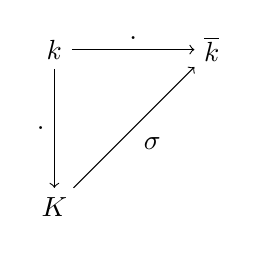
\begin{tikzpicture}[node distance=2cm, auto]
		\node (k) {$k$};
		\node (kk) [right of=k] {$\overline{k}$};
		\node (K) [below of=k] {$K$};

		\draw[->] (k) to node {$.$} (kk);
		\draw[->] (k) to node[swap] {$.$} (K);
		\draw[->] (K) to node[swap] {$\sigma$} (kk);

	\end{tikzpicture}
	\end{figure}

	\item $K$ é corpo de raízes sobre $k$ de uma família $(f_i)_{i \in I}$ de polinômios em $k[x] \setminus k$;
	\item Se $f \in k[x] \setminus k$ é irredutível em $k[x]$ com raiz $\alpha$, então $f(x)=c(x-\alpha_1)\cdots(x-\alpha_n)$ em $k[x]$, com $\alpha_1=\alpha$ e $c \in k \setminus \{0\}$.
	\end{enumerate}
\end{teo}
%\begin{proof}
%PULEI, tem nas notas mas não tudo.
%\end{proof}

\begin{defi}
	Uma extensão de corpos $k \subseteq K$ é uma \emph{extensão normal} se ela satisfaz uma das três condições do teorema acima.
\end{defi}

OBS: Se $k \subseteq \overline{k}$ é uma extensão algébrica, então todo $\beta \in \overline{k}$ é algébrico sobre $k$ vale para $\beta \in K$, então $k \subseteq K$ é extensão algébrica.

	Se $k \subseteq K$ é extensão algébrica, então $k \subseteq K \subseteq \overline{K}$ são extensões algébricas, então $k \subseteq \overline{K}$ é extensão algébrica. Então $\overline{k} \sim \overline{K}$ é fecho algébrico de $k$.

%(?????)

\begin{prop}
	Seja $k \subseteq K$ um extensão algébrica e $\sigma: K \to K$ um homomorfismo de cropos que satisfaz $\sigma|_k=id|_k$. Então $\sigma$ é um isomorfismo de corpos.
\end{prop}
%\begin{proof}
%...
%\end{proof}

\begin{defi}
	Seja $E \subseteq F$ uma extensão algébrica e $\sigma:E \to L$ um homomorfismo de corpos tal que $L$ é algebricamente fechaado, $\sigma(E) \subseteq L$ é uma extensão algébrica ($L$ é fecho algébrico de $\sigma(E)$)
	\begin{equation*}
	S_\sigma := \{\mu : \mu: F \to L \text{\ homomorfismo de corpos}, \mu|_E=\sigma\}.
	\end{equation*}
\end{defi}

\begin{lema}
	$|S_\sigma|$ depende de $E \subseteq F$, mas não depende de $\sigma$ nem de $L$.
\end{lema}
%\begin{proof}
%... vários diagramas
%\end{proof}

\begin{defi}
	Seja $E \subseteq F$ uma extensão algébrica. O \emph{grau de separabilidade} da extensão é $[F:E]_S := |S_\sigma|$. (Pode escolher $l=\overline{E}$ e $\sigma$ inclusão.)
\end{defi}

\begin{teo}
	\begin{enumerate}
	\item $E \subseteq F \subseteq K$ extensões algébricas, então
		\begin{equation*}
		[K:E]_S = [K:F]_S[F:E]_S
		\end{equation*}
	\item $E \subseteq F$ extensão finita (logo algébrica), então
		\begin{equation*}
		[F:E]_S \leq [F:E]
		\end{equation*}
	\end{enumerate}
\end{teo}
%\begin{proof}
%...
%\end{proof}

\begin{defi}
	Seja $E \subseteq K$ uma extensão finita. Ela é \emph{separável} se $[K:E]_S=[K:E]$.
\end{defi}

\begin{coro}
	Sejam $E \subseteq F \subseteq K$ extensões de corpos, $[K:E] < \infty$, $E \subseteq K$ separável. Então $E \subseteq F$ e $F subseteq K$ são separáveis.
\end{coro}
\begin{proof}
	\begin{equation*}
	[K:F]_S [F:E]_S = [K:E]_S = [K:E] = [K:F][F:E].
	\end{equation*}
	Como $[F:E]_S \leq [F:E]$ e $[K:F]_S \leq [K:F]$, segue o corolário.
\end{proof}

\section{Matrizes}

\begin{defi}
	Seja $\bm A$ um anel e $l,c \in \N$. Uma \emph{matriz} de dimensão $l \times c$ sobre $\bm A$ é uma função $M: [l] \times [c] \to A$. Representa-se isso por
	\begin{equation*}
	M =
	\begin{bmatrix}
	m_{1,1} & \cdots & m_{1,c} \\
	\vdots & \ddots & \vdots \\
	m_{l,1} & \cdots & m_{l,c}
	\end{bmatrix},
	\end{equation*}
em que $m_{i,j} := M(i,j) \in A$. O conjunto $[l]$ é o conjunto dos \emph{índices das linhas} e $[c]$ é o conjunto dos \emph{índices das colunas} da matriz $M$. A imagem de $M$ é o conjunto das \emph{entradas} da matriz $M$ e o elemento $m_{i,j}$ é a entrada da linha $i$ e coluna $j$.

	O conjunto de todas as matrizes de dimensão $l \times c$ sobre $\bm A$ é denotado por $\M_{l \times c}(\bm A)$.
\end{defi}

\begin{defi}
	Seja $\bm A$ um anel e $d \in \N$. Uma \emph{matriz quadrada} de dimensão $d$ sobre $\bm A$ é uma matriz $M \in \M_{d \times d}(\bm A)$. O conjunto de todas as matrizes quadradas de dimensão $d$ sobre $\bm A$ é denotado por $\M_d(\bm A)$.
\end{defi}

\begin{defi}
	Sejam $\bm A$ um anel e $M \in \M_{l \times c}(\bm A)$. A \emph{matriz transposta} de $M$ é a matriz $M^\intercal \in \M_{c \times l}(\bm A)$ definida por
	\begin{equation*}
	(M^\intercal)(i,j) := m_{j,i}.
	\end{equation*}
\end{defi}

\subsection{Soma de Matrizes}

\begin{defi}
	Sejam $\bm A$ um anel e $M,N \in \M_{l \times c}(\bm A)$. A \emph{matriz soma} das matrizes $M$ e $N$ é a matriz $(M+N) \in \M_{l \times c}(\bm A)$ definida por
	\begin{equation*}
	(M+N)(i,j) := m_{i,j}+n_{i,j}.
	\end{equation*}
\end{defi}

\begin{defi}
	Sejam $\bm A$ um anel e $0$ o elemento neutro da soma de $\bm A$.
	\begin{enumerate}
	\item A \emph{matriz nula} de dimensão $l \times c$ sobre $\bm A$ é a matriz $\zero_{l \times c} \in \M_{l \times c}(\bm A)$, definida por
		\begin{equation*}
		\zero_{l \times c}(i,j) := 0.
		\end{equation*}
	\item Se $M \in \M_{l \times c}$, a \emph{matriz negativa} de $M$ é a matriz $-M \in \M_{l \times c}(\bm A)$, definida por
		\begin{equation*}
		(-M)(i,j) := -m_{i,j}.
		\end{equation*}
	\end{enumerate}
\end{defi}

\begin{prop}
	Seja $\bm A$ um anel e $+$ a operação binária em $\M_{l \times c}(\bm A)$ definida por
	\begin{align*}
	\func{+}{\M_{l \times c}(\bm A) \times \M_{l \times c}(\bm A)}{\M_{l \times c}(\bm A)}{(M,N)}{M+N.}
	\end{align*}
Então $(\M_{l \times c}(\bm A),+)$ é um grupo com elemento neutro $\zero_{l \times c}$. Se $\bm A$ é comutativo, então $(\M_{l \times c}(\bm A),+)$ é comutativo.
\end{prop}
\begin{proof}
	Sejam $M,N,P \in \M_{l \times c}(\bm A)$. Primeiro, notemos que $+$ é associativa, pois, como a soma no anel é associativa, segue que
	\begin{equation*}
	(m_{i,j}+n_{i,j})+p_{i,j} = m_{i,j}+(n_{i,j}+p_{i,j})
	\end{equation*}
e, portanto, $(M+N)+P=M+(N+P)$. Então, notemos que $\zero$ é elemento neutro de $+$. Como $0$ é elemento neutro da soma da anel, segue que
	\begin{equation*}
	m_{i,j}+0 = 0+m_{i,j} = m_{i,j}
	\end{equation*}
e, portanto, $M+\zero=\zero+M=M$. Ainda, notemos que, como $-m_{i,j}$ é o inverso aditivo de $m_{i,j}$ no anel, segue que
	\begin{equation*}
	m_{i,j}+(-m_{i,j}) = (-m_{i,j})+m_{i,j} = 0
	\end{equation*}
e, portanto, $M+(-M)=(-M)+M=\zero$.	Assim, concluímos que $(\M_{l \times c}(\bm A),+)$ é um anel. Por fim, notemos que, se $\bm A$ é comutativo, então $+$ é comutativa, pois, como a soma no anel é comutativa, segue que
	\begin{equation*}
	m_{i,j}+n_{i,j} = n_{i,j}+m_{i,j}
	\end{equation*}
e, portanto, $M+N=N+M$. Assim, concluímos que, se $\bm A$ é comutativo, então $(\M_{l \times c}(\bm A),+)$ é comutativo.
\end{proof}

\subsection{Produto de Matrizes e Produto Por Escalar}

\begin{defi}
	Sejam $\bm A$ um anel e $M \in \M_{l \times d}(\bm A)$ e $N \in \M_{d \times c}(\bm A)$. A \emph{matriz produto} das matrizes $M$ e $N$ é a matriz $(MN) \in \M_{l \times c}(\bm A)$ definida por
	\begin{equation*}
	(MN)(i,j) := \sum_{k=1}^d m_{i,k}n_{k,j}.
	\end{equation*}
\end{defi}

\begin{prop}
	Sejam $\bm A$ um anel e $M \in \M_{l \times d_1}(\bm A)$, $N \in \M_{d_1 \times d_2}(\bm A)$ e $P \in \M_{d_2 \times c}(\bm A)$. Então
	\begin{equation*}
	(MN)P = M(NP).
	\end{equation*}
\end{prop}
\begin{proof} Um elemento de $MN$ é dado por
	\begin{equation*}
	(mn)_{i,j} = \sum_{k_1=1}^{d_1} m_{i,k_1}n_{k_1,j}.
	\end{equation*}
Logo, um elemento de $(MN)P$ é dado por
	\begin{equation*}
	((mn)p)_{i,j} = \sum_{k_2=1}^{d_2} (mn)_{i,k_2}p_{k_2,j} = \sum_{k_2=1}^{d_2} \left(\sum_{k_1=1}^{d_1} m_{i,k_1}n_{k_1,k_2}\right)p_{k_2,j}.
	\end{equation*}
Analogamente, um elemento de $M(NP)$ é dado por
	\begin{equation*}
	(m(np))_{i,j} = \sum_{k_1=1}^{d_1} m_{i,k_1}(np)_{k_1,j} = \sum_{k_1=1}^{d_1} m_{i,k_1}\left(\sum_{k_2=1}^{d_2} n_{k_1,k_2}p_{k_2,j}\right).
	\end{equation*}
Mas então, como $\bm A$ é um anel, segue que
	\begin{align*}
	((mn)p)_{i,j}
	&= \sum_{k_2=1}^{d_2} \left(\sum_{k_1=1}^{d_1} m_{i,k_1}n_{k_1,k_2}\right)p_{k_2,j} \\
	&= \sum_{k_2=1}^{d_2} \left(\sum_{k_1=1}^{d_1} m_{i,k_1}n_{k_1,k_2}p_{k_2,j}\right) \\
	&= \sum_{k_1=1}^{d_1} \left(\sum_{k_2=1}^{d_2} m_{i,k_1}n_{k_1,k_2}p_{k_2,j}\right) \\
	&= \sum_{k_1=1}^{d_1} m_{i,k_1}\left(\sum_{k_2=1}^{d_2} n_{k_1,k_2}p_{k_2,j}\right) \\
	&= (m(np))_{i,j}.
	\end{align*}
\end{proof}

\begin{defi}
	Sejam $\bm A$ um anel e $0$ e $1$ os elementos neutros da soma e da multiplicação de $\bm A$ respectivamente. A \emph{matriz identidade} de dimensão $d$ sobre $\bm A$ é a matriz $\id_d \in \M_d(\bm A)$ definida por
	\begin{equation*}
	\id_d(i,j) := \delta_{i,j} =
		\begin{cases}
			1 & i = j \\
			0 & i \neq j,
		\end{cases}
	\end{equation*}
\end{defi}

Essa função $\delta$ é conhecida como delta de Kronecker.

\begin{prop}
	Seja $\bm A$ um anel e $\cdot$ a operação binária em $\M_d(\bm A)$ definida por
	\begin{align*}
	\func{\cdot}{\M_d(\bm A) \times \M_d(\bm A)}{\M_d(\bm A}{(M,N)}{MN.}
	\end{align*}
Então $(\M_d(\bm A),\cdot)$ é um monoide com elemento neutro $\id_d$.
\end{prop}
\begin{proof}
	Sejam $M,N,P \in \M_d(\bm A)$. Pela proposição anterior, sabemos que vale $(MN)P=M(NP)$ e que, portanto, $\cdot$ é associativa. Agora, notemos que um elemento de $M\id_d$ é da forma
	\begin{equation*}
	\sum_{k=0}^{d-1} m_{i,k}\delta_{k,j}.
	\end{equation*}
Mas, para $k \in [d]$, se $k \neq j$, então $\delta_{k,j}=0$ e, se $k=j$, então $\delta_{k,j}=1$ e, portanto, segue que
	\begin{equation*}
	\sum_{k=1}^d m_{i,k}\delta_{k,j} = m_{i,j}.
	\end{equation*}
Assim, concluímos que $M\id_d=M$. Analogamente, mostra-se que $\id_dM=M$, e concluímos que $\id_d$ é elemento neutro de $\cdot$. Isso mostra que $(\M_d(\bm A),\cdot)$ é um monoide.
\end{proof}

\begin{defi}
	Seja $\bm A$ um anel. Uma \emph{matriz invertível} é uma matriz $M \in \M_d(\bm A)$ que é invertível com respeito ao produto do monoide $(\M_d(\bm A),\cdot)$. A matriz inversa de $M$ é denotada $M^{-1}$.
\end{defi}

\begin{defi}
	Seja $\bm A$ um anel, $a \in A$ e $M \in \M_{l \times c}(\bm A)$. O \emph{produto por escalar} de $a$ e $M$ é a matriz $aM \in \M_{l \times c}$ definida por
	\begin{equation*}
	(aM)(i,j) := am_{i,j}.
	\end{equation*}
\end{defi}

\subsection{Matrizes Quadradas}

\begin{defi}
	Seja $\bm A$ um anel.
	\begin{enumerate}
	\item Uma \emph{matriz triangular superior} é uma matriz quadrada $M \in \M_d(\bm A)$ que satisfaz
		\begin{equation*}
		\forall i,j \in [d] \qquad i > j \Rightarrow m_{i,j}=0.
		\end{equation*}
	\item Uma \emph{matriz triangular inferior} é uma matriz quadrada $M \in \M_d(\bm A)$ sobre $\bm A$ que satisfaz
		\begin{equation*}
		\forall i,j \in [d] \qquad i < j \Rightarrow m_{i,j}=0.
		\end{equation*}
	\item Uma \emph{matriz triangular superior} é uma matriz quadrada $M \in \M_d(\bm A)$ que satisfaz
		\begin{equation*}
		\forall i,j \in [d] \qquad i > j \Rightarrow m_{i,j}=0.
		\end{equation*}
	\item Uma \emph{matriz triangular} é uma matriz quadrada $M \in \M_d(\bm A)$ que é triangular superior ou triangular inferior.
	\item Uma \emph{matriz diagonal} é uma matriz quadrada $M \in \M_d(\bm A)$ que é triangular superior e triangular inferior; ou seja, que satisfaz
		\begin{equation*}
		\forall i,j \in [d] \qquad i \neq j \Rightarrow m_{i,j}=0.
		\end{equation*}
	\item Uma \emph{matriz simétrica}  uma matriz quadrada $M \in \M_d(\bm A)$ que é igual a sua transposta
		\begin{equation*}
		M = M^\intercal.
		\end{equation*}
	\item Uma \emph{matriz antissimétrica} é uma matriz quadrada $M \in \M_d(\bm A)$ que é igual à negativa da sua transposta
		\begin{equation*}
		M = -M^\intercal.
		\end{equation*}
	\item Uma \emph{matriz ortogonal} é uma matriz quadrada $M \in \M_d(\bm A)$ cuja transposta é igual à sua inversa
		\begin{equation*}
		M^\intercal = M^{-1}.
		\end{equation*}
	\end{enumerate}
\end{defi}

\subsection{Traço e Determinante}

\begin{defi}
	Sejam $\bm A$ um anel e $M \in \M_d(\bm A)$. O \emph{traço} de $M$ é o elemento $\tr(M) \in A$ definido por
	\begin{equation*}
	\tr(M) := \sum_{i=1}^d m_{i,i}.
	\end{equation*}
\end{defi}

\begin{prop}
	Sejam $\bm A$ um anel, $a \in A$ e $M,N \in \M_d(\bm A)$. Então
	\begin{enumerate}
	\item $\tr(M^\intercal)=\tr(M)$;
	\item $\tr(MN)=\tr(NM)$;
	\item $\tr(M+N)=\tr(M)+\tr(N)$;
	\item $\tr(aM)=a\tr(M)$.
	\end{enumerate}
\end{prop}
\begin{proof}
	\begin{enumerate}
	\item
		\begin{equation*}
		\tr(M) = \sum_{i=1}^d m_{i,i} = \tr(M^\intercal).
		\end{equation*}
	\item
		\begin{align*}
		\tr(MN) &= \sum_{i=1}^d \left(\sum_{k=1}^d m_{i,k}n_{k,i}\right) \\
		&= \sum_{i=1}^d \left(\sum_{k=1}^d n_{k,i}m_{i,k}\right) \\
		&= \sum_{k=1}^d \left(\sum_{i=1}^d n_{k,i}m_{i,k}\right) \\
		&= \tr(NM).
		\end{align*}
	\item
		\begin{align*}
		\tr(M+N) &= \sum_{i=1}^d (m_{i,i} + n_{i,i}) \\
		&= \sum_{i=1}^d m_{i,i} + \sum_{i=1}^d n_{i,i} \\
		&= \tr(M) + \tr(N).
		\end{align*}
	\item
		\begin{equation*}
		\tr(aM) = \sum_{i=1}^d am_{i,i} = a\sum_{i=1}^d m_{i,i} = a\tr(M).
		\end{equation*}
\qedhere
	\end{enumerate}
\end{proof}
























\chapter{Corpos}

\section{Corpo e Subcorpo}

Já demos a definição de um corpo no capítulo de anéis, mas agora pretendemos ressaltar essa definição.

\begin{defi}
Um \emph{corpo} é uma lista $\bm C = (C,+,-,0,\times,\inv,1)$ tal que
	\begin{enumerate}
	\item $(C,+,-,0,\times,1)$ é um anel;
	\item $(C \setminus \{0\},\times,\inv,1)$ é um grupo (comutativo).
	\end{enumerate} 
\end{defi}

\section{Corpo de Frações}

\begin{defi}
Seja $\bm D$ um domínio. A \emph{equivalência de frações} em $D \times D \setminus \{0\}$ é a relação definida por: para todos $(n,d),(n',d') \in D \times D*$,
	\begin{equation*}
	(n,d) \sim (n',d') \Leftrightarrow nd' = dn'.
	\end{equation*}
\end{defi}

\begin{prop}
Seja $\bm D$ um domínio. A \emph{equivalência de frações} em $D \times D \setminus \{0\}$ é uma equivalência.
\end{prop}
\begin{proof}
(Reflexividade) Segue direto de $nd=dn$ para todo $(n,d) \in D \times D \setminus \{0\}$.

(Simetria) Segue direto de $nd'=dn'$ se, e somente se, $dn'=nd'$ para todos $(n,d),(n',d') \in D \times D*$.

(Transitividade) Sejam $(n,d),(n',d'),(n'',d'') \in D \times D \setminus \{0\}$ tais que $(n,d) \sim (n',d')$ e $(n',d') \sim (n'',d'')$. Isso significa que $nd' = dn'$ e $n'd'' = d'n''$. Então segue que
	\begin{equation*}
	d'(nd'') = nd'd'' = dn'd'' = dd'n'' = d'(dn'')
	\end{equation*}
logo, como $d \neq 0$, segue da propriedade de cancelamento que
	\begin{equation*}
	nd'' = dn'',
	\end{equation*}
o que significa que $(n,d) \sim (n'',d'')$.
\end{proof}

Note que a transitividade exige que valha a prorpiedade de cancelamente, por isso precisamos de um domínio, e também exige a comutatividade da multiplicação. Como essa relação é uma equivalência, podemos considerar o quociente desse conjunto pela relação, e obtemos o que se chama corpo de frações.

\begin{defi}
Seja $\bm D$ um domínio. O \emph{corpo de frações} de $\bm D$ é o conjunto
	\begin{equation*}
	Q(D) := \quo{D \times D \setminus \{0\}}{\sim}.
	\end{equation*}
Os elementos de $Q(D)$ são \emph{frações} e são denotadas
	\begin{equation*}
	\frac{n}{d} := [(n,d)].
	\end{equation*}
A \emph{adição de frações} é a função
	\begin{align*}
	\func{+}{Q(D) \times Q(D)}{Q(D)}{\left( \frac{n}{d},\frac{n'}{d'} \right)}{\frac{nd'+dn'}{dd'}}
	\end{align*}
A \emph{inversa da adição de frações} é a função
	\begin{align*}
	\func{-}{Q(D)}{Q(D)}{\frac{n}{d}}{\frac{-n}{d}}
	\end{align*}
A \emph{nulidade de frações} é a fração
	\begin{equation*}
	0 := \frac{0}{1}.
	\end{equation*}
A \emph{multiplicação de frações} é a função
	\begin{align*}
	\func{+}{Q(D) \times Q(D)}{Q(D)}{\left( \frac{n}{d},\frac{n'}{d'} \right)}{\frac{nn'}{dd'}};
	\end{align*}
A \emph{inversa da multiplicação de frações} é a função
	\begin{align*}
	\func{\inv}{Q(D) \setminus \{0\}}{Q(D) \setminus \{0\}}{\frac{n}{d}}{\frac{d}{n}};
	\end{align*}
A \emph{unidade de frações} é a fração
	\begin{equation*}
	1 := \frac{1}{1}.
	\end{equation*}
\end{defi}

\begin{defi}
Seja $\bm D$ um domínio. A lista $(Q(D),+,-,0,\times,\inv,1)$ é um corpo.
\end{defi}
\begin{proof}
Exercício simples.
\end{proof}

\begin{defi}
Seja $\bm D$ um domínio. A \emph{inclusão canônica} de $D$ em $Q(D)$ é a função
	\begin{align*}
	\func{\inclu}{D}{Q(D)}{a}{\frac{a}{1}}.
	\end{align*}
\end{defi}

\begin{prop}
Seja $\bm D$ um domínio. A inclusão $\iota\colon D \to Q(D)$ é um homomorfismo injetivo de anéis.
\end{prop}

\begin{prop}[Propriedade Universal]
\label{alg:prop.univer.corpo.frac}
Sejam $\bm D$ um domínio, $\bm C$ um corpo e $h\colon D \to C$ um homomorfismo injetivo de anel. Existe um único homomorfismo injetivo de anel $\bar h\colon Q(D) \to C$ tal que $\bar h \circ \iota = h$ (o diagrama comuta).
\begin{figure}
\centering
\begin{tikzpicture}[node distance=2.5cm, auto]
	\node (C) {$\bm D$};
	\node (G) [above of=C] {$\displaystyle\bm{Q(D)}$};
	\node (X) [right of=C] {$\bm C$};
	\draw[->] (C) to node [swap] {$h$} (X);
	\draw[->, dashed] (G) to node {$\bar h$} (X);
	\draw[->] (C) to node {$\iota$} (G);
\end{tikzpicture}
\end{figure}
\end{prop}
\begin{proof}
Definimos
	\begin{align*}
	\func{\bar h}{Q(D)}{C}{\frac{n}{d}}{h(n)h(d)\inv}.
	\end{align*}
Mostremos primeiro que essa função está bem definida. Primeiro, note que, como $h$ é injetiva e $d \neq 0$, então $h(d) \neq 0$, portanto existe $h(d)\inv \in C$. Agora, sejam $(n,d),(n',d') \in D \times D \setminus \{0\}$ tais que $\frac{n}{d} = \frac{n'}{d'}$. Então $nd'=dn'$, e segue da injetividade de $h$ vale que $h(nd') = h(dn')$. Mas então $h(n)h(d')=h(d)h(n')$, o que implica que $h(n)h(d)\inv = h(n')h(d')\inv$, e segue que
	\begin{equation*}
	\bar h\left( \frac{n}{d} \right) = h(n)h(d)\inv = h(n')h(d')\inv = \bar h\left( \frac{n'}{d'} \right).
	\end{equation*}

Agora mostremos que $\bar h$ é homomorfismo de anel. (Homomorfismo de grupo) Sejam $\frac{n}{d},\frac{n'}{d'} \in Q(D)$. Então
	\begin{align*}
	\bar h\left( \frac{n}{d} + \frac{n'}{d'} \right) &= \bar h\left( \frac{nd'+dn'}{dd'} \right) \\
		&= h(nd'+dn')h(dd')\inv \\
		&= (h(n)h(d')+h(d)h(n'))h(d)\inv h(d')\inv \\
		&= h(n)h(d)\inv + h(n')h(d')\inv \\
		&= \bar h\left( \frac{n}{d} \right) + \bar h \left( \frac{n'}{d'} \right).
	\end{align*}

(Homomorfismo de monoide) Sejam $\frac{n}{d},\frac{n'}{d'} \in Q(D)$. Então
	\begin{align*}
	\bar h\left( \frac{n}{d}\frac{n'}{d'} \right) &= \bar h\left( \frac{nn'}{dd'} \right) \\
		&= h(nn')h(dd')\inv \\
		&= h(n)h(n')h(d)\inv h(d')\inv \\
		&= h(n)h(d)\inv h(n')h(d')\inv \\
		&= \bar h\left( \frac{n}{d} \right)\bar h \left( \frac{n'}{d'} \right).
	\end{align*}
Ainda, como $h$ é homomorfismo de anel, $h(1)=1$, logo
	\begin{equation*}
	\bar h\left( \frac{1}{1} \right) = h(1)h(1)\inv = 1.
	\end{equation*}

(Injetividade) Sejam $\frac{n}{d},\frac{n'}{d'} \in Q(D)$ tais que $\bar h(\frac{n}{d}) = \bar h(\frac{n'}{d'})$. Então
	\begin{align*}
	0 &= \bar h \left( \frac{n}{d} \right) - \bar h \left( \frac{n'}{d'} \right) \\
		&= \bar h \left( \frac{n}{d} - \frac{n'}{d'} \right) \\
		&= \bar h \left( \frac{nd'-dn'}{dd'} \right) \\
		&= h(nd'-dn')h(dd')\inv.
	\end{align*}
Como $d \neq 0$ e $d' \neq 0$, segue que $h(nd'-dn')=0$, e da injetividade de $h$ segue que $nd'-dn'=0$, logo $nd'=dn'$, o que significa que $\frac{n}{d} = \frac{n'}{d'}$.

%(Unicidade) Seja $g\colon Q(D) \to C$ um homomorfismo injetivo de anel tal que $g \circ \iota = h$. Então, para todos $m$
\end{proof}


\subsection{Os Números Racionais \ensuremath{\Q}}

Essa construção, aplicada ao anel dos números inteiro, é o conjunto dos números racionais.

\begin{defi}
$\Q : = Q(\Z)$.
\end{defi}














\subsection{Funções de Arredondamento}


\subsubsection{Chão e teto}

\begin{defi}
A função \emph{chão} é a função
	\begin{align*}
	\func{\chao{\var}}{\R}{\Z}{x}{\max\set{i \in \Z}{i \leq x}}.
	\end{align*}
A função \emph{teto} é a função
	\begin{align*}
	\func{\teto{\var}}{\R}{\Z}{x}{\min\set{i \in \Z}{i \geq x}}.
	\end{align*}
\end{defi}

\begin{prop}
Para todo $x \in \R$,
	\begin{enumerate}
	\item (Conjugação)
		\begin{align*}
		-\chao{x} &= \teto{-x} \\
		-\teto{x} &= \chao{-x};
		\end{align*}
	\item (Idempotência)
		\begin{align*}
		\chao{\chao{x}} &= \chao{x} \\
		\teto{\teto{x}} &= \teto{x};
		\end{align*}
	\end{enumerate}
\end{prop}



\begin{prop}
Para todo $x, x' \in \R$ e todo $i \in \Z$,
	\begin{enumerate}
	\item
		\begin{align*}
		\chao{x+i} &= \chao{x}+i \\
		\teto{x+i} &= \teto{x}+i;
		\end{align*}

	\item
		\begin{align*}
		\chao{x}+\chao{x'} &\leq \chao{x+x'} \leq \chao{x}+\chao{x'}+1 \\
		-1+\teto{x}+\teto{x'} &\leq \teto{x+x'} \leq \teto{x}+\teto{x'};
		\end{align*}
	\end{enumerate}
\end{prop}



\begin{prop}
Para todos $x,x' \in \R$, $x'>0$ e todos $i,i' \in \Z$, $i>0$,
	\begin{enumerate}
	\item 
		\begin{align*}
		\chao{\frac{\chao{x}+i'}{i}} &= \chao{\frac{x+i'}{i}} \\
		\teto{\frac{\teto{x}+i'}{i}} &= \teto{\frac{x+i'}{i}};
		\end{align*}

	\item
		\begin{align*}
		\teto{\frac{i'}{i}} - 1 &= \chao{\frac{i'-1}{i}} \\
		\chao{\frac{i'}{i}} + 1 &= \teto{\frac{i'+1}{i}};
		\end{align*}

	\item	
		\begin{align*}
		\chao{\frac{\chao{x \div x'}}{i}} &= \chao{\frac{x}{x'i}} \\	
		\teto{\frac{\teto{\frac{x}{x'}}}{i}} &= \teto{\frac{x}{x'i}}.
		\end{align*}
	
	\end{enumerate}
\end{prop}




\subsubsection{Resto e parte fracionária}

\begin{defi}
Sejam $x,y \in \R$, $x' \neq 0$. O \emph{resto} de $x$ com respeito a $x'$ é
	\begin{equation*}
	\resto{x}{x'} := x - x'\chao{\frac{x}{x'}}.
	\end{equation*}
A \emph{parte fracionária} de $x$ é o resto de $x$ com respeito a $1$:
	\begin{equation*}
	\resfra{x} := \resto{x}{1}.
	\end{equation*}
\end{defi}

\begin{prop}
Sejam $x,x' \in \R$, $x' \neq 0$.
	\begin{enumerate}
	\item Se $x'>0$,
		\begin{equation*}
		0 \leq \resto{x}{x'} < x';
		\end{equation*}

	\item Se $x'<0$,
		\begin{equation*}
		x' < \resto{x}{x'} \leq 0;
		\end{equation*}
	\end{enumerate}
\end{prop}





\begin{prop}
Seja $x \in \R$,
	\begin{equation*}
	\teto{\resfra{x}} = \teto{x} - \chao{x} = \begin{cases}
			0,& x \in \Z \\
			1,& x \notin \Z.
		\end{cases}
	\end{equation*}
\end{prop}


\begin{prop}
Sejam $x \in \R$, $i \in \Z$, $i > 0$.
	\begin{equation*}
	\teto{\resfra{ \frac{x}{i} }} = \teto{\frac{x}{i}} - \chao{\frac{x}{i}}  = \begin{cases}
			0,& x \in i\Z \\
			1,& x \notin i\Z.
		\end{cases}
	\end{equation*}
\end{prop}


\subsubsection{Arredondamento}

\begin{defi}
A função \emph{arredondamento meio para baixo} é a função
	\begin{align*}
	\func{\arrebai{\var}}{\R}{\Z}{x}{\teto{x-\frac{1}{2}}}.
	\end{align*}
A função \emph{arredondamento meio para cima} é a função
	\begin{align*}
	\func{\arrecim{\var}}{\R}{\Z}{x}{\chao{x+\frac{1}{2}}}.
	\end{align*}
\end{defi}









\chapter{Espaços Lineares}

\section{Módulos}

\begin{defi}
Seja $\bm A=(A,+,-,0,\cdot,1)$ um anel. Um \emph{módulo (à esquerda)} sobre $\bm A$ é um par $(\bm M,\bm \cdot)$ em que $\bm M=(M,\bm +,\bm -,\bm 0)$ é um grupo comutativo e $\bm \cdot\colon \bm A \age \bm M$ é uma ação de anel ($\bm \cdot\colon \bm A \to \End(\bm M)$ é um homomorfismo de anel); ou seja,
	\begin{enumerate}
	\item  Para todo $a \in A$, a função $a \bm \cdot\colon \bm M \to \bm M$ é um homomorfismo de grupo:
		\begin{enumerate}
		\item Para todos $m_0,m_1 \in M$,
			\begin{equation*}
			a \bm \cdot (m_0 \bm + m_1) = a \bm \cdot m_0 \bm + a \bm \cdot m_1.
			\end{equation*}
		\end{enumerate}
	\item $\bm \cdot \colon A \times M \to M$ é uma ação de anel:
		\begin{enumerate}
		\item Para todos $a_0,a_1 \in A$ e $m \in M$,
			\begin{equation*}
			(a_0 + a_1) \bm \cdot m = a_0 \bm \cdot m + a_1 \bm \cdot m;
			\end{equation*}
%			\begin{equation*}
%			(a_0 + a_1) \bm \cdot = (a_0 \bm \cdot) + (a_1 \bm \cdot)
%			\end{equation*}
		\item Para todos $a_0,a_1 \in A$ e $m \in M$,
			\begin{equation*}
			(a_0 \cdot a_1) \bm \cdot m = a_0 \bm \cdot (a_1 \bm \cdot m);
			\end{equation*}
%			\begin{equation*}
%			(a_0 \cdot a_1) \bm \cdot = (a_0 \bm \cdot) \circ (a_1 \bm \cdot)
%			\end{equation*}
		\item Para todo $m \in M$,
			\begin{equation*}
			1 \bm \cdot m = m;
			\end{equation*}
%			\begin{equation*}
%			1 \bm \cdot = \Id
%			\end{equation*}
		\end{enumerate}
	\end{enumerate}
Os símbolos da operação $\cdot$ de $\bm A$ e da ação $\bm \cdot$ serão suprimidos (e parênteses desnecessários relacionados a elas também), e os símbolos das operações $+,-$ de $\bm A$ e $\bm +,\bm -$ de $\bm M$ não serão diferenciadas em notação, nem os das constantes $0 \in A$ e $\bm 0 \in M$.
\end{defi}

Na definição usamos o fato de que $\End(\bm M)$ é um anel com as operações puxadas para o espaço de funções, a soma pontual sendo a soma do anel e a composição de função sendo o produto. De fato, se $X$ é um conjunto e $\bm G$ um grupo comutativo, o conjunto $G^X$ de funções de $X$ para $G$, com a soma pontual e a composição, é um anel, e basta mostrar que quando $X=G$, o conjunto $\End(\bm G)$ de endomorfismos de grupo de $\bm G$ é um subanel de $G^G$.

\begin{prop}
Sejam $X$ um conjunto e $\bm G$ um grupo comutativo. Então
	\begin{equation*}
	(G^X,+,-,0,\circ,\Id)
	\end{equation*}
é um anel.
\end{prop}
\begin{proof}
	\begin{enumerate}
	\item $(G^X,+,-,0)$ é um grupo comutativo.
		\begin{enumerate}
		\item Para todos $f_0,f_1,f_2 \in G^X$ e $x \in X$,
			\begin{align*}
			((f_0+f_1)+f_2)(x) &= (f_0+f_1)(x)+f_2(x) \\
				&= (f_0(x)+f_1(x))+f_2(x) \\
				&= f_0(x)+(f_1(x)+f_2(x)) \\
				&= f_0(x)+(f_1+f_2)(x) \\
				&= (f_0+(f_1+f_2))(x);
			\end{align*}
		\item Para todos $f \in G^X$ e $x \in X$,
			\begin{align*}
			(0+f)(x) &= 0(x)+f(x) \\
				&= 0+f(x) \\
				&= f(x) \\
				&= f(x)+0 \\
				&= f(x)+0(x) \\
				&= (f+0)(x);
			\end{align*}
		\item Para todos $f \in G^X$ e $x \in X$,
			\begin{align*}
			((-f)+f)(x) &= (-f)(x)+f(x) \\
				&= -f(x)+f(x) \\
				&= 0 \\
				&= f(x)+(-f(x)) \\
				&= f(x) + (-f)(x) \\
				&= (f+(-f))(x);				
			\end{align*}
		\item Para todos $f_0,f_1 \in G^X$ e $x \in X$,
			\begin{align*}
			(f_0+f_1)(x) = f_0(x)+f_1(x) = f_1(x) + f_0(x) = (f_1+f_0)(x).
			\end{align*}
		\end{enumerate}
	
	\item $(G^X,\circ,\Id)$ é um monoide.
		\begin{enumerate}
		\item Para todos $f_0,f_1,f_2 \in G^X$ e $x \in X$,
			\begin{align*}
			((f_0 \circ f_1) \circ f_2)(x) &= (f_0 \circ f_1)(f_2(x)) \\
				&= (f_0(f_1(f_2(x))) \\
				&= f_0((f_1 \circ f_2)(x)) \\
				&= (f_0 \circ (f_1 \circ f_2))(x);
			\end{align*}
		\item Para todos $f \in G^X$ e $x \in X$,
			\begin{align*}
			(\Id \circ f)(x) = \Id(f(x)) = f(x) = f(\Id(x)) = (f \circ \Id)(x).
			\end{align*}
		\end{enumerate}
	\item A composição $\circ$ é distributiva à esquerda e à direita sobre a soma pontual $+$.
		\begin{enumerate}
		\item Para todos $f,f_0,f_1 \in G^X$ e $x \in X$,
			\begin{align*}
			(f \circ (f_0+f_1))(x) &= f((f_0+f_1)(x)) \\
				&= f(f_0(x)+f_1(x)) \\
				&= f(f_0(x))+f(f_1(x)) \\
				&= (f \circ f_0)(x) + (f \circ f_1)(x);
			\end{align*}
		\item Para todos $f_0,f_1,f \in G^X$ e $x \in X$,
			\begin{align*}
			((f_0+f_1) \circ f)(x) &= (f_0+f_1)(f(x)) \\
				&= f_0(f(x)) + f_1(f(x)) \\
				&= (f_0 \circ f)(x) + (f_1 \circ f)(x).
			\end{align*}
		\end{enumerate}
	\end{enumerate}
\end{proof}

\begin{prop}
Seja $\bm G$ um grupo comutativo. Então
	\begin{equation*}
	(\End(G),+,-,0,\circ,\Id)
	\end{equation*}
é um anel.
\end{prop}
\begin{proof}
Como $\End(\bm G) \subseteq G^G$, basta mostrar que $\End(\bm G)$ é subanel de $G^G$.
	\begin{enumerate}
	\item $\End(\bm G)$ é subgrupo.
		\begin{enumerate}
		\item Para todos $h_0,h_1 \in \End(\bm G)$ e $g_0,g_1 \in G$,
			\begin{align*}
			(h_0+h_1)(g_0+g_1) &= h_0(g_0+g_1) + h_1(g_0+g_1) \\
				&= h_0(g_0) + h_0(g_1) + h_1(g_0) + h_1(g_1) \\
				&= h_0(g_0) + h_1(g_0) + h_0(g_1) + h_1(g_1) \\
				&= (h_0 + h_1)(g_0) + (h_0 + h_1)(g_1);
			\end{align*}
		\item Para todos $h \in \End(\bm G)$ e $g_0,g_1 \in G$,
			\begin{align*}
			(-h)(g_0+g_1) &= -h(g_0+g_1) \\
				&= -(h(g_0)+h(g_1)) \\
				&= -h(g_0)-h(g_1) \\
				&= (-h)(g_0)+(-h)(g_1).
			\end{align*}
		\end{enumerate}
	\item $\End(\bm G)$ é submonoide.
		\begin{enumerate}
		\item Para todos $h_0,h_1 \in \End(\bm G)$ e $g_0,g_1 \in G$,
			\begin{align*}
			(h_0 \circ h_1)(g_0+g_1) &= h_0(h_1(g_0+g_1)) \\
				&= h_0(h_1(g_0)+h_1(g_1)) \\
				&= h_0(h_1(g_0))+h_0(h_1(g_1)) \\
				&= (h_0 \circ h_1)(g_0)+h_0 \circ h_1)(g_1);
			\end{align*}
		\item Para todos $g_0,g_1 \in G$,
			\begin{align*}
			\Id(g_0+g_1) = g_0+g_1 = \Id(g_0)+\Id(g_1).
			\end{align*}
		\end{enumerate}
	\end{enumerate}
\end{proof}

\section{Espaço e Subespaço Lineares}

\begin{defi}
Seja $\bm C=(C,+,-,0,\cdot,1)$ um corpo. Um \emph{espaço linear} sobre $\bm C$ é um módulo $(\bm V,\bm \cdot)$ sobre $\bm C$; ou seja,
	\begin{enumerate}
	\item  Para todo $c \in C$, a função $c \bm \cdot \colon \bm V \to \bm V$ é um homomorfismo de grupo:
		\begin{enumerate}
		\item Para todos $v_0,v_1 \in M$,
			\begin{equation*}
			c \bm \cdot (v_0 \bm + v_1) = c \bm \cdot v_0 \bm + c \bm \cdot v_1.
			\end{equation*}
		\end{enumerate}
	\item $\bm \cdot \colon C \times V \to V$ é uma ação de corpo (ou de anel):
		\begin{enumerate}
		\item Para todos $c_0,c_1 \in C$ e $v \in V$,
			\begin{equation*}
			(c_0 + c_1) \bm \cdot v = c_0 \bm \cdot v + c_1 \bm \cdot v;
			\end{equation*}
		\item Para todos $c_0,c_1 \in C$ e $v \in V$,
			\begin{equation*}
			(c_0 \cdot c_1) \bm \cdot v = c_0 \bm \cdot (c_1 \bm \cdot v);
			\end{equation*}
		\item Para todo $v \in V$,
			\begin{equation*}
			1 \bm \cdot v = v;
			\end{equation*}
		\end{enumerate}
	\end{enumerate}
Os símbolos da operação $\cdot$ de $\bm C$ e da ação $\bm \cdot$ serão suprimidos (e parênteses desnecessários relacionados a elas também), e os símbolos das operações $+,-$ de $\bm C$ e $\bm +,\bm -$ de $\bm V$ não serão diferenciadas em notação.
%, nem os das constantes $0 \in C$ e $\bm 0 \in V$.
Um espaço linear será denotado como $\bm V$ quando não for relevante explicitar a ação $\bm \cdot$.
\end{defi}

%\begin{defi}
%Um \emph{espaço linear} (ou \emph{espaço vetorial}) sobre um corpo $\bm C=(C,+,\cdot)$ é um módulo $\bm V=(\bm V, \bm \cdot)$ sobre $\bm C$; mais detalhadamente, é uma tripla $\bm V = (V, \bm +, \bm \cdot)$ em que
%	\begin{enumerate}
%	\item $(V,\bm +)$ é um grupo comutativo com elemento neutro $\bm 0$;
%	\item $\bm \cdot: C \times V \to V$ é uma função que satisfaz
%		\begin{enumerate}
%		\item $\forall \bm v \in V \qquad 1\bm\cdot \bm v=\bm v$;
%		\item $\forall c_1,c_2 \in C \ \forall \bm v \in V \qquad (c_1 \cdot c_2) \bm\cdot \bm v = c_1 \bm\cdot(c_2 \bm\cdot \bm v)$;
%		\item $\forall c \in C \ \forall \bm v_1,\bm v_2 \in V \qquad c \bm\cdot (\bm v_1 \bm + \bm v_2) = c \bm\cdot \bm v_1 \bm + c\bm\cdot \bm v_2$;
%		\item $\forall c_1,c_2 \in C \ \forall \bm v \in V \qquad (c_1+c_2) \bm\cdot \bm v = c_1 \bm{\cdot v} \bm + c_2\bm{\cdot v}$.
%		\end{enumerate}
%	\end{enumerate}
%Os elementos de $V$ são \emph{vetores} e denotados em negrito e os elementos de $C$ são \emph{escalares}. As operações $\bm +$ e $\bm \cdot$ do espaço linear são denotadas por $+$ e $\cdot$, o inverso de $\bm v \in V$ é denotado $-\bm v$ e a imagem de $(c,\bm v) \in C \times V$ é o \emph{produto} de $c$ e $\bm v$ e é denotada por $c\bm v$. Quando o corpo é $\R$, dizemos \emph{espaço vetorial real}; quando o corpo é $\C$, dizemos \emph{espaço vetorial complexo}.
%\end{defi}

\begin{prop}
Seja $\bm V$ um espaço linear sobre um corpo $\bm C$. Para todos $\bm v \in V$ e $c \in C$,
	\begin{enumerate}
	\item $c\bm v = \bm 0 \Leftrightarrow c=0 \ou \bm v = \bm 0$;
	\item $-(c\bm v) = (-c)\bm v = c(- \bm v)$;
	\item $c\bm v = (-c)(- \bm v)$.
	\end{enumerate}
\end{prop}
\begin{proof} Sejam $\bm v \in V$ e $c \in C$.
	\begin{enumerate}
	\item Primeiro, notemos que
		\begin{align*}
		0 \bm v &= 0 \bm v + \bm 0 \\
			&= 0 \bm v + (0 \bm v - 0 \bm v) \\
			&= (0 \bm v + 0 \bm v) - 0 \bm v \\
			&= (0+0) \bm v - 0 \bm v \\
			&= 0 \bm v - 0 \bm v \\
			&= \bm 0.
		  \end{align*}
Agora, notemos que
		\begin{align*}
		c \bm 0 &= c \bm 0 + \bm 0 \\
			&= c \bm 0 + (c \bm 0 - c \bm 0) \\
			&= (c \bm 0 + c \bm 0) - c \bm 0 \\
			&= c  (\bm 0 + \bm 0) - c \bm 0 \\
			&= c \bm 0 - c \bm 0 \\
			&= \bm 0.
		\end{align*}
Portanto, se $c=0$ ou $\bm v = \bm 0$, então $c\bm v = \bm 0$. Agora, suponhamos que $c\bm v =\bm 0$. Se $c \neq 0$, como $\bm C$ é corpo, segue da demonstração anterior que
		\begin{equation*}
		\bm v = c^{-1}c\bm v = c^{-1} \bm 0 = \bm 0.
		\end{equation*}
	\item Basta notar que
		\begin{align*}
		\bm -(c\bm{v}) &= \bm -(c\bm{v}) + \bm 0 \\
			&= \bm -(c\bm{v}) + (0 \bm v) \\
			&= \bm -(c\bm{v}) + (c-c) \bm v \\
			&= \bm -(c\bm{v}) + (c\bm v + (-c) \bm v) \\
			&= (\bm -(c\bm{v}) + c\bm v) + (-c) \bm v \\
			&= \bm 0 + (-c) \bm v \\
			&= (-c) \bm v
		\end{align*}
e que
		\begin{align*}
		-(c\bm{v}) &= -(c\bm{v}) + \bm 0 \\
			&= -(c\bm v) + (c \bm 0) \\
			&= -(c\bm v) + c(\bm v - \bm v) \\
			&= -(c\bm v) + (c\bm v + c(- \bm v)) \\
			&= (-(c\bm v + c\bm v) + c(- \bm v) \\
			&= \bm 0 + c(- \bm v) \\
			&= c(- \bm v).
		\end{align*}
	\item Do item anterior, segue que
		\begin{equation*}
		c\bm v = (-(-c))\bm v = (-c)(- \bm v).  \qedhere
		\end{equation*}
	\end{enumerate}
\end{proof}

\begin{prop}
Seja $\bm C$ um corpo e $n$ um natural positivo. Então $(C^n,+,\bm\cdot)$, em que
	\begin{align*}
	\func{\bm\cdot}{C \times C^n}{C^n}{(c,(c_1,\ldots,c_n))}{(c \cdot c_1,\ldots,c \cdot c_n),}
	\end{align*}
é um espaço vetorial sobre $\bm C$.
\end{prop}
\begin{proof}
	Claramente $(C^n,+)$ é um grupo comutativo com elemento neutro $(0,\ldots,0)$. Note que, para todos $(c_1,\ldots,c_n) \in C^n$ e $c,c' \in C$,
	\begin{equation*}
	1 \bm\cdot (c_1,\ldots,c_n) = (1 \cdot c_1,\ldots,1 \cdot c_n) = (c_1,\ldots,c_n)
	\end{equation*}
e
	\begin{align*}
	(c \cdot c') \bm\cdot (c_1,\ldots,c_n) &= ((c \cdot c') \cdot c_1, \ldots, (c \cdot c') \cdot c_n) \\
	&= ((c \cdot (c' \cdot c_1), \ldots, (c \cdot (c' \cdot c_n)) \\
	&= c \bm\cdot (c' \cdot c_1,\ldots,c' \cdot c_n) \\
	&= c \bm\cdot (c' \bm\cdot (c_1,\ldots,c_n)).
	\end{align*}
	Ainda, note que, para todos $(c_1,\ldots,c_n), (c'_1,\ldots,c'_n) \in C^n$ e $c,c' \in C$,
	\begin{align*}
	c \bm\cdot ((c_1,\ldots,c_n) + (c'_1,\ldots,c'_n)) &= c \bm\cdot (c_1+c'_1,\ldots,c_n+c'_n) \\
	&= (c \cdot (c_1+c'_1),\ldots,c \cdot (c_n+c'_n)) \\
	&= (c \cdot c_1 + c \cdot c'_1,\ldots,c \cdot c_n + c \cdot c'_n) \\
	&= (c \cdot c_1,\ldots,c \cdot c_n) + (c \cdot c'_1,\ldots,c \cdot c'_n) \\
	&= c \bm\cdot (c_1,\ldots,c_n) + c \bm\cdot (c'_1,\ldots,c'_n)
	\end{align*}
e
	\begin{align*}
	(c+c') \bm\cdot (c_1,\ldots,c_n) &= ((c+c')c_1,\ldots,(c+c')c_n) \\
	&= (c \cdot c_1 + c' \cdot c_1,\ldots,c \cdot c_n + c' \cdot c_n)_{i \in I} \\
	&= (c \cdot c_1,\ldots,c \cdot c_n) + (c' \cdot c_1,\ldots,c' \cdot c_n) \\
	&= c \bm\cdot (c_1,\ldots,c_n) + c' \bm\cdot (c_1,\ldots,c_n).  \qedhere
	\end{align*}
\end{proof}

Para generalizar esse resultado, lembremos que o produto de uma família $(C_i)_{i \in I}$ de conjuntos é $\prod_{i \in I} C_i$ e, quando $C_i=C$, temos que $\prod_{i \in I} C_i = C^I$ e os elementos de $C^I$ são funções $c=(c_i)_{i \in I}$ de $I$ em $C$.

\begin{prop}
Sejam $I$ um conjunto e $\bm C$ um corpo. Então $\bm {C^I}=(C^I,\bm +,\bm\cdot)$, em que
	\begin{align*}
	\func{\bm +}{C^I}{C^I}{(\bm c,\bm c')}{(c_i+c'_i)_{i \in I}}
	\end{align*}
e
	\begin{align*}
	\func{\bm\cdot}{C \times C^I}{C^I}{(a,\bm c)}{(a \cdot c_i)_{i \in I}}
	\end{align*}
é um espaço vetorial sobre $\bm C$.
\end{prop}

Esse exemplo pode ser ainda mais generalizado como a seguir.

%%%%%%%%%%%%%%%%%%%%%%%%%%%%%%%%%%%%%%%%%%%%
\begin{comment}
\begin{prop}[Espaço de Funções]
Sejam $\bm V$ e $\bm W$ espaços vetoriais sobre um corpo $\bm C$. Então $\bm{W^V}=(W^V,+,\cdot)$, em que
	\begin{align*}
	\func{+}{W^V \times W^V}{W^V}{(\bm f_1,\bm f_2)}{
		\begin{aligned}[t]
		\func{\bm f_1+\bm f_2}{V}{W}{\bm v}{\bm f_1(\bm v)+\bm f_2(\bm v).}
		\end{aligned}
	}
	\end{align*}
e
\begin{align*}
	\func{\cdot}{C \times W^V}{W^V}{(c,\bm f)}{
		\begin{aligned}[t]
		\func{c\bm f}{V}{W}{\bm v}{c\bm f(\bm v),}
		\end{aligned}
	}
	\end{align*}
é um espaço vetorial sobre $\bm C$.
\end{prop}
\begin{proof}
Primeiro, sabemos que $(W^V,+)$ é um grupo comutativo com identidade $0: W^V \times W^V \to W^V$ definida por $0(\bm v)=0$. Devemos então mostrar que $\cdot: C \times W^V \to W^V$ satisfaz os itens da definição de espaço vetorial. Primeiro, seja $\bm f \in W^V$. Então, para todo $\bm v \in V$, $(1\bm f)(\bm v)=1\bm f(\bm v)=\bm f(\bm v)$, o que mostra que $1\bm f=\bm f$. Agora, sejam $c_1,c_2 \in C$ e $\bm f \in W^V$. Então, para todo $\bm v \in V$,
	\begin{equation*}
	((c_1c_2)\bm f)(\bm v) = (c_1c_2)\bm f(\bm v) = c_1(c_2\bm f(\bm v)) = c_1(c_2\bm f)(\bm v) = (c_1(c_2\bm f))(\bm v),
	\end{equation*}
o que mostra que $(c_1c_2)\bm f=c_1(c_2\bm f)$.

Por fim, devemos mostrar as propriedades distributivas. Sejam $c \in C$ e $\bm f_1,\bm f_2 \in W^V$. Então, para todo $\bm v \in V$,
	\begin{align*}
	(c(\bm f_1+\bm f_2))(\bm v)&=c(\bm f_1+\bm f_2)(\bm v) \\
	&=c(\bm f_1(\bm v)+\bm f_2(\bm v)) \\
	&= c\bm f_1(\bm v)+c \bm f_2(\bm v) \\
	&= (c\bm f_1)(\bm v)+(c \bm f_2)(\bm v) \\
	&=(c\bm f_1+c \bm f_2)(\bm v),
	\end{align*}
o que mostra que $c(\bm f_1+\bm f_2)=c\bm f_1+c \bm f_2$. Agora, sejam $c_1,c_2 \in C$ e $\bm f \in W^V$. Então, para todo $\bm v \in V$,
	\begin{align*}
	((c_1+c_2)\bm f)(\bm v) &= (c_1+c_2) \bm f(\bm v) \\
	&=c_1\bm f(\bm v)+c_2\bm f(\bm v) \\
	&=(c_1\bm f)(\bm v)+(c_2\bm f)(\bm v) \\
	&=(c_1\bm f+c_2\bm f)(\bm v),
	\end{align*}
o que mostra que $(c_1+c_2)\bm f=c_1\bm f+c_2\bm f$. Assim, concluímos que $(W^V,+,\cdot)$ é um espaço vetorial sobre $\bm C$.
\end{proof}
\end{comment}
%%%%%%%%%%%%%%%%%%%%%%%%%%%%%%%%%%%%%%%%%%%%

\begin{prop}[Espaço de Funções]
Sejam $X$ um conjunto e $\bm V$ um espaço vetorial sobre um corpo $\bm C$. Então $\bm{V^X}=(V^X,+,\cdot)$, em que
	\begin{align*}
	\func{+}{V^X \times V^X}{V^X}{(\bm f_1,\bm f_2)}{
		\begin{aligned}[t]
		\func{\bm f_1+\bm f_2}{X}{V}{x}{\bm f_1(x)+\bm f_2(x).}
		\end{aligned}
	}
	\end{align*}
e
\begin{align*}
	\func{\cdot}{C \times V^X}{V^X}{(c,\bm f)}{
		\begin{aligned}[t]
		\func{c\bm f}{X}{V}{x}{c\bm f(x),}
		\end{aligned}
	}
	\end{align*}
é um espaço vetorial sobre $\bm C$.
\end{prop}
\begin{proof}
Primeiro, sabemos que $(V^X,+)$ é um grupo comutativo com identidade $0\colon V^X \times V^X \to V^X$ definida por $0(x)=0$. Devemos então mostrar que $\cdot\colon C \times V^X \to V^X$ satisfaz os itens da definição de espaço vetorial. Primeiro, seja $\bm f \in V^X$. Então, para todo $x \in X$, $(1\bm f)(x)=1\bm f(x)=\bm f(x)$, o que mostra que $1\bm f=\bm f$. Agora, sejam $c_1,c_2 \in C$ e $\bm f \in V^X$. Então, para todo $x \in X$,
	\begin{equation*}
	((c_1c_2)\bm f)(x) = (c_1c_2)\bm f(x) = c_1(c_2\bm f(x)) = c_1(c_2\bm f)(x) = (c_1(c_2\bm f))(x),
	\end{equation*}
o que mostra que $(c_1c_2)\bm f=c_1(c_2\bm f)$.

Por fim, devemos mostrar as propriedades distributivas. Sejam $c \in C$ e $\bm f_1,\bm f_2 \in V^X$. Então, para todo $x \in X$,
	\begin{align*}
	(c(\bm f_1+\bm f_2))(x)&=c(\bm f_1+\bm f_2)(x) \\
	&=c(\bm f_1(x)+\bm f_2(x)) \\
	&= c\bm f_1(x)+c \bm f_2(x) \\
	&= (c\bm f_1)(x)+(c \bm f_2)(x) \\
	&=(c\bm f_1+c \bm f_2)(x),
	\end{align*}
o que mostra que $c(\bm f_1+\bm f_2)=c\bm f_1+c \bm f_2$. Agora, sejam $c_1,c_2 \in C$ e $\bm f \in V^X$. Então, para todo $x \in X$,
	\begin{align*}
	((c_1+c_2)\bm f)(x) &= (c_1+c_2) \bm f(x) \\
	&=c_1\bm f(x)+c_2\bm f(x) \\
	&=(c_1\bm f)(x)+(c_2\bm f)(x) \\
	&=(c_1\bm f+c_2\bm f)(x),
	\end{align*}
o que mostra que $(c_1+c_2)\bm f=c_1\bm f+c_2\bm f$. Assim, concluímos que $(V^X,+,\cdot)$ é um espaço vetorial sobre $\bm C$.
\end{proof}

\begin{defi}
	Seja $\bm V$ um espaço vetorial sobre um corpo $\bm C$. Um \emph{subespaço vetorial} de $\bm V$ é um conjunto não vazio $W \subseteq V$ tal que
	\begin{enumerate}
	\item $\forall \bm w_1,\bm w_2 \in W \qquad \bm w_1 + \bm w_2 \in W$;
	\item $\forall c \in C \ \forall \bm w \in W \qquad c \bm w \in W$.
	\end{enumerate}
\end{defi}

\begin{prop}
	Seja $\bm V=(V,+,\cdot)$ um espaço vetorial sobre um corpo $\bm C$. Então um conjunto não vazio $W \subseteq V$ é um subespaço vetorial de $\bm V$ se, e somente se, $\bm W=(W,+|_{W \times W},\cdot|_{C \times W})$ é um espaço vetorial sobre $\bm C$.
\end{prop}

\begin{prop}
	Seja $\bm V$ um espaço vetorial sobre um corpo $\bm C$ e $W$ um subespaço vetorial de $\bm V$. Então
	\begin{enumerate}
	\item $\bm 0 \in W$;
	\item $\{\bm 0\}$ e $V$ são subespaços vetoriais de $\bm V$.
	\end{enumerate}
\end{prop}
\begin{proof}
	\begin{enumerate}
	\item Como $W$ não é vazio, seja $\bm w \in W$. Então $0 \bm w = \bm 0 \in W$.
	\item Seja $W=\{\bm 0\}$. Se $\bm w_1,\bm w_2 \in W$, $\bm w_1 = \bm 0$ e $\bm w_2 =\bm 0$, e segue que $\bm w_1 + \bm w_2 = \bm 0 + \bm 0 = \bm 0$. Ainda, para todo $c \in C$, segue que $c\bm w_1 = c\bm 0=\bm 0 \in W$.
	Seja $W=V$. Como $\bm V$ é espaço vetorial, então $V$ é subespaço vetorial de $\bm V$ pala proposição anterior. \qedhere
	\end{enumerate}
\end{proof}

\begin{prop}
	Sejam $\bm V$ um espaço vetorial sobre um corpo $\bm C$ e $(W_i)_{i \in I}$ uma família de subespaços vetoriais de $\bm V$. Então
	\begin{equation*}
	W := \bigcap_{i \in I} W_i
	\end{equation*}
é um subespaço vetorial de $\bm V$.
\end{prop}
\begin{proof}
	Como, para todo $i \in I$, $\bm 0 \in W_i$, segue que $\bm 0 \in W$ e, portanto, $W$ não é vazio. Agora, sejam $\bm w_1,\bm w_2 \in W$ e $c \in C$. Então, para todo $i \in I$, $\bm w_1,\bm w_2 \in W_i$ e, como $W_i$ é subespaço vetorial de $\bm V$, segue que $\bm w_1+\bm w_2 \in W_i$ e que $c\bm w_1 \in W_i$. Logo $\bm w_1+\bm w_2 \in W$ e $c\bm w_1 \in W$, o que mostra que $W$ é subespaço vetorial de $\bm V$.
\end{proof}

\begin{prop}
	Sejam $\bm V$ um espaço vetorial sobre um corpo $\bm C$ e $\{W_i\}_{i \in I}$ uma cadeia de subespaços vetoriais de $\bm V$ (ou seja, para todos $I,j \in I$, $W_I \subseteq W_j$ ou $W_j \subseteq W_i$). Então
	\begin{equation*}
	W := \bigcup_{i \in I} W_i
	\end{equation*}
é um subespaço vetorial de $\bm V$.
\end{prop}
\begin{proof}
	Como, para todo $i \in I$, $\bm 0 \in W_i$, pois $W_i$ é subespaço vetoriasl de $\bm V$, segue que $\bm 0 \in W$ e, portanto, $W$ não é vazio. Agora, sejam $\bm w_1,\bm w_2 \in W$. Então existem $i,j \in I$ tais que $\bm w_1 \in W_i$ e $\bm w_2 \in W_j$. Nesse caso, $W_i \subseteq W_j$ ou $W_j \subseteq W_i$. Sem perda de generalidade, suponhamos o primeiro caso. Então segue que $\bm w_1 \in W_j$ e, portanto, $\bm w_1+\bm w_2 \in W_j$, o que mostra que $\bm w_1+\bm w_2 \in W$. Agora, seja $c \in C$ e notemos que, como $W_i$ é subespaço vetorial de $\bm V$, segue que $c\bm w_1 \in W_i$. Logo $c\bm w_1 \in W$, o que mostra que $W$ é subespaço vetorial de $\bm V$.
\end{proof}

\begin{defi}
	Sejam $\bm V$ um espaço vetorial sobre um corpo $\bm C$, $W \subseteq V$ e $(W_i)_{i \in I}$ uma indexação do conjunto de todos subespaços vetoriais de $\bm V$ dos quais $W$ é subconjunto. O \emph{subespaço vetorial gerado por $W$} em $\bm V$ é o subespaço vetorial
	\begin{equation*}
	\langle W \rangle := \bigcap_{i \in I} W_i.
	\end{equation*}
Nesse caso, dizemos que $W$ é um \emph{conjunto gerador} de $\langle W \rangle$ ou que $W$ gera $\langle W \rangle$.

% Caso $W$ seja finito, $W = \{\bm w_1, \ldots, \bm w_n \}$, escrevemos $\langle W \rangle = \langle \bm w_1, \ldots, \bm w_n \rangle$.

\end{defi}

\begin{prop}
	Sejam $\bm V$ um espaço vetorial sobre um corpo $\bm C$. Então $\langle \emptyset \rangle = \{\bm 0\}$.
\end{prop}
\begin{proof}
	Como $\{\bm  0\}$ é um subespaço vetorial de $V$ e $\emptyset \subseteq \{\bm 0\}$, segue que, se $\bm v \in \langle \emptyset \rangle$, então $\bm v \in \{\bm 0\}$, o que implica $\bm v = \bm 0$ e, portanto, que $\langle \emptyset \rangle = \{\bm 0\}$.
\end{proof}

\section{Combinação Linear de Vetores}

\begin{defi}
	Sejam $\bm V$ um espaço vetorial sobre um corpo $\bm C$ e $W \subseteq V$ um conjunto finito tal que $W=\{\bm w_1,\ldots,\bm w_n\}$. Uma \emph{combinação linear} de $W$ em $\bm V$ é um vetor $\bm v \in V$ tal que existem $c_1,\ldots,c_n \in C$ satisfazendo
	\begin{equation*}
	\bm v = \sum_{i=1}^n c_i\bm w_i.
	\end{equation*}
Se $W$ é um conjunto infinito, uma \emph{combinação linear} de $W$ é uma combinação linear de um subconjunto finito de $W$.


\end{defi}

 O vetor $\bm 0$ é combinação linear de qualquer conjunto, pois é a soma vazia.

\begin{teo}
	Sejam $\bm V$ um espaço vetorial sobre um corpo $\bm C$ e $W \subseteq V$ não vazio. Então $\langle W \rangle$ é o conjunto de todas as combinações lineares de $W$ em $\bm V$.
\end{teo}
\begin{proof}
	Consideremos, primeiro, o caso em que $W=\emptyset$. Nesse caso, $\langle W \rangle = \{\bm 0\}$, e a única combinação linear de $W$ é a soma vazia $\bm 0$, o que mostra a igualdade dos conjuntos.

	Agora, assumamos que $W \neq \emptyset$ e seja $(W_j)_{j \in J}$ uma indexação do conjunto de todos subespaços de $\bm V$ que contêm $W$. Primeiro, mostraremos que uma combinação linear de $W$ em $\bm V$ está em $\langle W \rangle$. Seja $\bm v := \sum_{i=1}^n c_i\bm w_i$ uma combinação linear de $W$ em $\bm V$. Para todo $j \in J$, $W_j$ é um subespaço vetorial de $\bm V$. Portanto, para todo $i \in [n]$, segue que $c_i \bm{w_i} \in W_j$ e, então, que $\bm v \in W_j$. Logo $\bm v \in \langle W \rangle$.

	Reciprocamente, mostraremos que o conjunto de todas combinações lineares de $W$ em $\bm V$ é um subespaço vetorial de $\bm V$. Primeiro, notemos que $\bm 0$ é uma combinação linear de $W$, pois, para todo $\bm w \in W$, vale $\bm 0 = 0\bm w$. Agora, sejam $\bm v_1 = \sum_{i=1}^n c_i\bm w_i$ e $\bm v_2 = \sum_{i=1}^m c'_i\bm w'_i$ combinações lineares de $W$ em $\bm V$ e $c \in C$. Então, se definirmos, para todo $i \in [m]$, $\bm w_{n+i} := \bm w'_i$ e $c_{n+i} := c'_i$ e, para todo $i \in [n]$, $\overline c_i := cc_i$, segue que
	\begin{equation*}
	\bm v_1 + \bm v_2 = \sum_{i=1}^n c_i\bm w_i + \sum_{i=1}^m c'_i\bm w'_i = \sum_{i=1}^{n+m} c_i\bm w_i
	\end{equation*}
e
	\begin{equation*}
	c\bm v_1 = \sum_{i=1}^n (cc_i)\bm w_i = \sum_{i=1}^n \overline c_i \bm w_i
	\end{equation*}
são combinações lineares de $W$ em $\bm V$, o que implica que o conjunto de todas combinações lineares de $W$ em $\bm V$ é um subespaço de $\bm V$. Assim, como $\langle W \rangle$ é subconjunto de todo conjunto que é subespaço vetorial de $\bm V$ contendo $W$, segue que o conjunto de todas combinações lineares de $W$ em $\bm V$ é igual ao subespaço gerado por $W$.
\end{proof}

\begin{prop}
	Sejam $\bm V$ um espaço vetorial sobre um corpo $\bm C$, $W \subseteq V$ e $\bm v \in \langle W \rangle$. Então existem $\bm w_1, \ldots, \bm w_n \in W$ distintos e $c_1, \ldots, c_n \in C$ tais que
	\begin{equation*}
	\bm v = \sum_{i=1}^n c_i \bm w_i.
	\end{equation*}
\end{prop}
\begin{proof}
	Como $\bm v \in \langle W \rangle$, existem $\bm w'_1, \ldots, \bm w'_m \in W$ e $c'_1, \ldots, c'_m \in C$ tais que $\bm v = \sum_{i=1}^m c'_i \bm w'_i$. Vamos particionar o conjunto dos índices $[m]$ com a seguinte relação de equivalência: para todo $i,j \in [m]$, $i \sim j$ se, e somente se, $\bm w'_i = \bm w'_j$. Essa relação é de equivalência pois a igualddade de vetores é uma relação de equivalência. Agora, seja $n$ o número de classes de equivalências dessa relação. Para cada $i \in [n]$, seja $j \in P_i$ e definimos os vetores $\bm w_i := \bm w'_j$. Notemos que os vetores $\bm w_i$ estão bem definidos, não dependem do $j$, pois, se $k \in P_i$, então $\bm w_i = \bm w'_j = \bm w'_k$. Ainda, definimos os coeficientes $c_i := \sum _{j \in P_i} c'_j$. Desse modo, segue que
	\begin{equation*}
	\bm v = \sum_{i=1}^m c'_i \bm w'_i = \sum_{i=1}^n \sum_{j \in P_i} c'_j \bm w'_j = \sum_{i=1}^n \sum_{j \in P_i} c'_j \bm w_i =  \sum_{i=1}^n c_i \bm w_i.
	\end{equation*}
	Por fim, notemos que os $\bm w_1, \ldots, \bm w_n$ são distintos por definição, já que, se $\bm w_i = \bm w_j$ para $i,j \in [n]$, então existem $k,l \in [m]$ tais que $k \in P_i$, $l \in P_j$ e $\bm w_i = \bm w'_k$, $\bm w_j = \bm w'_l$. Mas isso implica $\bm w'_k=\bm w'_l$, o que implica $P_i = P_j$ e, portanto, $i = j$.
\end{proof}

\begin{defi}[Dependência Linear]
	Sejam $\bm V$ um espaço vetorial sobre um corpo $\bm C$ e $W \subseteq V$. Dizemos que $W$ é \emph{linarmente dependente} em $\bm V$ se existem $\bm w_1, \ldots,\bm w_n \in W$ distintos e $c_1,\ldots,c_n \in C$ não nulos tais que
	\begin{equation*}
	\bm 0 = \sum_{i=1}^n c_i \bm w_i.
	\end{equation*}
Caso contrário, dizemos que $W$ é \emph{linearmente independente} em $\bm V$.
\end{defi}

\begin{prop}
	Sejam $\bm V$ um espaço vetorial sobre um corpo $\bm C$ e $W \subseteq V$. Então $W$ é linearmente dependente se, e somente se, existe $\bm w \in W$ que é combinação linear de $W \setminus \{\bm w\}$ em $\bm V$.
\end{prop}
\begin{proof}
	Suponhamos que $W$ é linearmente dependente. Então existem vetores $\bm w'_1,\ldots,\bm w'_n \in W$ distintos e $c'_1,\ldots,c'_n \in C$ não nulos tais que
	\begin{equation*}
	\bm 0 = \sum_{i=1}^n c'_i \bm w'_i.
	\end{equation*}
Como $c'_1,\ldots,c'_n$ são não nulos, então existe $j \in [n]$ tal que $c'_j \neq 0$. Definindo $\bm w_i := \bm w'_i$ se $1 \leq i < j$ e $\bm w_i := \bm w'_{i-1}$ se $j < i \leq n$, e $c_i := (c'_j)^{-1}(-c'_i)$ para todo $1 \leq i < j$ ou $j < i \leq n$, segue que
	\begin{equation*}
	\bm w'_j = \sum_{i=1}^{j-1} (c'_j)^{-1}(-c'_i) \bm w'_i + \sum_{i=j+1}^n (c'_j)^{-1}(-c'_i) \bm w'_i = \sum_{i=1}^{n-1} c_i \bm w_i.
	\end{equation*}
Por tanto, como $\bm w_i \in W \setminus \{\bm w'_j\}$ e $c_i \in C$ para todo $i \in [n-1]$, $\bm w'_j$ é combinação linear de $W \setminus \{\bm w'_j\}$ em $\bm V$.

	Reciprocamente, suponhamos que existe $\bm w \in W$ que é combinação linear de $W \setminus \{\bm w\}$ em $\bm V$. Então existem $\bm w_1, \ldots, \bm w_n \in W \setminus \{\bm w\}$ distintos e $c_1, \ldots, c_n \in C$ tais que
	\begin{equation*}
	\bm w = \sum_{i=1}^n c_i \bm w_i.
	\end{equation*}
Definindo $\bm w_{n+1} := \bm w$ e $c_{n+1} := -1$, segue que
	\begin{equation*}
	\bm 0 = \sum_{i=1}^n c_i \bm w_i - \bm w = \sum_{i=1}^{n+1} c_i \bm w_i.
	\end{equation*}
Então, como $\bm w_1, \ldots, \bm w_{n+1}$ são distintos e $c_{n+1} = -1 \neq 0$, segue que $W$ é linearmente dependente.
\end{proof}

\begin{prop}
	Sejam $\bm V$ um espaço vetorial sobre um corpo $\bm C$ e $W \subseteq V$. Então
	\begin{enumerate}
	\item $\emptyset$ é linearmente independente em $\bm V$;
	\item Se $\bm 0 \in W$, então $W$ é linearmente dependente em $\bm V$;
	\item Se $W=\{\bm v\}\neq\{\bm 0\}$, então $W$ é linearmente independente em $\bm V$.
	\item Sejam $\bm v,\bm v' \neq 0$. $W = \{\bm v,\bm v'\}$ é linearmente dependente se, e somente se, existe $c \in C \setminus \{0\}$ tal que $\bm v' = c\bm v$.
	\end{enumerate}
\end{prop}
\begin{proof}
	\begin{enumerate}
	\item Suponha, por absurdo, que $\emptyset$ não é linearmente independente. Então existem $\bm{w_1},\ldots,\bm{w_n} \in \emptyset$ distintos e $c_1,\ldots,c_n \in C$ não nulos tais que
	\begin{equation*}
	\bm 0 = \sum_{i=1}^n c_i\bm{w_i}.
	\end{equation*}
Mas $\bm{w_1},\ldots,\bm{w_n} \in \emptyset$ é um absurdo.
	\item Seja $c \in C \setminus \{0\}$. Então, como $\bm 0 = c \bm 0$, segue que $W$ é linearmente dependente em $\bm V$.
	\item Se $\bm 0 = c\bm v$, como $\bm v \neq \bm 0$, segue que $c=0$, o que mostra que $W$ é linearmente independente em $\bm V$.
	\item Se $W$ é linearmente dependente, então existem $c,c' \in C \setminus \{0\}$ tais que $0 = c\bm v + c' \bm v'$, o que implica que
		\begin{equation*}
		\bm v' = -\frac{c}{c'} \bm v.
		\end{equation*}
Reciprocamente, se existe $c \in C \setminus \{0\}$ tal que $\bm v' = c\bm v$, então
	\begin{equation*}
	0 = -c \bm v +c\bm v = -c \bm v + \bm v',
	\end{equation*}
o que mostra que $W$ é linearmente dependente.
	\end{enumerate}
\end{proof}

\begin{prop}
	Sejam $\bm V$ um espaço vetorial sobre um corpo $\bm C$ e $W \subseteq V$. Então $W$ é linearmente independente em $\bm V$ se, e somente se, para toda combinação linear $\bm v = \sum_{i=1}^n c_i\bm w_i \neq \bm 0$ de $W$ em $\bm V$ tal que $\bm w_1,\ldots,\bm w_n$ são distintos e não nulos, então $c_1,\ldots,c_n$ são únicos.
\end{prop}
\begin{proof}
	Primeiro, suponhamos que $W$ é linearmente dependente em $\bm V$. Então existem $\bm w'_1, \ldots,\bm w'_{n'} \in W$ distintos e $c'_1,\ldots,c'_{n'} \in C$ não nulos tais que
	\begin{equation*}
	\bm 0 = \sum_{i=1}^{n'} c'_i\bm w'_i.
	\end{equation*}
Nesse caso, seja $\bm v \in \langle W \rangle$. Se $\bm v = \bm 0$, então segue que









 .......................................... . Se $\bm v \neq \bm 0$










\end{proof}

\begin{prop}
	Sejam $\bm V$ um espaço vetorial sobre um corpo $\bm C$ e $\{W_i\}_{i \in I}$ uma cadeia de conjuntos linearmente independentes em $\bm V$ (ou seja, para todos $i,j \in I$, $W_i \subseteq W_j$ ou $W_j \subseteq W_i$). Então
	\begin{equation*}
	W := \bigcup_{i \in I} W_i
	\end{equation*}
é um conjunto linearmente independente em $\bm V$.
\end{prop}
\begin{proof}
	Como, para todo $i \in I$, $\bm 0 \in W_i$, segue que $\bm 0 \in W$ e, portanto, $W$ não é vazio. Agora, sejam $\bm w_1,\bm w_2 \in W$. Então existem $i,j \in I$ tais que $\bm w_1 \in W_i$ e $\bm w_2 \in W_j$. Nesse caso, $W_i \subseteq W_j$ ou $W_j \subseteq W_i$. Sem perda de generalidade, suponhamos o primeiro caso. Então segue que $\bm w_1 \in W_j$ e, portanto, $\bm w_1+\bm w_2 \in W_j$, o que mostra que $\bm w_1+\bm w_2 \in W$. Agora, seja $c \in C$ e notemos que, como $W_i$ é subespaço vetorial de $\bm V$, segue que $c\bm w_1 \in W_i$. Logo $c\bm w_1 \in W$, o que mostra que $W$ é subespaço vetorial de $\bm V$.
\end{proof}


\section{Soma de Subespaços Vetoriais}

\begin{defi}
	Sejam $\bm V$ um espaço vetorial sobre um corpo $\bm C$ e $(W_i)_{i \in I}$ uma família de subespaços vetoriais de $\bm V$. A \emph{soma} de $(W_i)_{i \in I}$ é o subespaço vetorial gerado pela união de $W_i$. Denotamos
	\begin{equation*}
	\sum_{i \in I} W_i := \left\langle \bigcup_{i \in I} W_i \right\rangle.
	\end{equation*}
Caso $(W_i)_{i \in I}$ seja uma família finita, escrevemos $W_1 + \cdots + W_n$.
\end{defi}

\begin{defi}
	Seja $\bm V$ um espaço vetorial sobre um corpo $\bm C$. Uma \emph{soma direta} é a soma de uma família $(W_i)_{i \in I}$ de subespaços vetoriais de $\bm V$ tal que $W_i \cap W_j = \{\bm 0\}$ para todo $i,j \in I$, $i \neq j$. Nesse caso, denotamos
	\begin{equation*}
	\bigoplus_{i \in I} W_i := \left\langle \bigcup_{i \in I} W_i\right\rangle.
	\end{equation*}
Caso $(W_i)_{i \in I}$ seja uma família finita, escrevemos $W_1 \oplus \cdots \oplus W_n$.
\end{defi}

\begin{prop}
	Seja $\bm V$ um espaço vetorial sobre um corpo $\bm C$ e $W_1,\ldots,W_n$ subespaços vetoriais de $\bm V$ tais que $V = \sum_{i=1}^n W_i$. Então
	\begin{equation*}
	V=\bigoplus_{i=1}^n W_i
	\end{equation*}
se, e somente se, para todo $\bm v \in V$, existem únicos $\bm w_1 \in W_1,\ldots,\bm w_n \in W_n$ tais que
	\begin{equation*}
	\bm v = \sum_{i=1}^n \bm w_i.
	\end{equation*}
\end{prop}
\begin{proof}
	Mostraremos, primeiro, que se $V$ é soma direta de $W_1,\ldots,W_n$, então todo vetor de $V$ é soma única de vetores de $W_1,\ldots,W_n$. A demontração será por indução em $n$. O caso base é trivial, pois, se $V=W_1$, então, para todo $\bm v \in V$, $\bm v \in W_1$. Agora, suponhamos que a proposição vale para todo natural menor ou igual a $n$. Sejam $W_1,\ldots,W_{n+1}$ subespaços vetoriais de $V$ tais que $V = \sum_{i=1}^{n+1} W_i$. Então existem $\bm w_1 \in W_1,\ldots,\bm w_{n+1} \in W_{n+1}$ tais que
	\begin{equation*}
	\bm v = \sum_{i=1}^{n+1} \bm w_i.
	\end{equation*}
Suponhamos que existam $\bm w_1 \in W_1,\ldots,\bm w_{n+1} \in W_{n+1}$ tais que
	\begin{equation*}
	\bm v = \sum_{i=1}^{n+1} \bm w'_i.
	\end{equation*}
Então
	\begin{equation*}
	\bm v = \sum_{i=1}^{n+1} \bm w_i = \sum_{i=1}^{n+1} \bm w'_i,
	\end{equation*}
o que implica
	\begin{equation*}
	\sum_{i=1}^n (\bm w_i - \bm w'_i) = \bm w'_{n+1} - \bm w_{n+1}.
	\end{equation*}
Como, para todo $i \in [n+1]$, $w_i,w'_i \in W_i$, segue que $\bm w_i - \bm w'_i \in W_i$. Definamos $W := \bigcup_{i=1}^n W_i$. Assim, segue que
	\begin{equation*}
	\sum_{i=1}^n (\bm w_i - \bm w'_i) \in \langle W \rangle
	\end{equation*}
e
	\begin{equation*}
	\bm w'_{n+1} - \bm w_{n+1} \in W_{n+1}.
	\end{equation*}
Ainda, como $V$ é soma direta de $W_1,\ldots,W_{n+1}$, então segue que $W \cap W_{n+1} = \{\bm 0\}$. Portanto concluímos que
	\begin{equation*}
	\sum_{i=1}^n (\bm w_i - \bm w'_i) = \bm w'_{n+1} - \bm w_{n+1} = \bm 0.
	\end{equation*}
Assim, concluímos que $\bm w'_{n+1}=\bm w_{n+1}$ e que
	\begin{equation*}
	\sum_{i=1}^n \bm w_i = \sum_{i=1}^n \bm w'_i.
	\end{equation*}
Mas notemos que
	\begin{equation*}
	\bm{\langle W \rangle}=(\langle W \rangle,+|_{\langle W \rangle \times \langle W \rangle},\cdot|_{\langle W \rangle \times \langle W \rangle})
	\end{equation*}
é um espaço vetorial e $W_1,\ldots,W_n$ são subespaços vetoriais de $\bm{\langle W \rangle}$ tais que $\langle W \rangle=\displaystyle\sum_{i=1}^n W_i$. Portanto, pela hipótese de indução, segue que, para todo $i \in [n]$, $\bm w_i = \bm w'_i$ e, portanto, concluímos que existem únicos $\bm w_1 \in W_1,\ldots,\bm w_{n+1} \in W_{n+1}$ tais que
	\begin{equation*}
	\bm v = \sum_{i=1}^{n+1} \bm w_i.
	\end{equation*}

	Suponhamos, então, que todo vetor de $V$ é soma de únicos vetores de $W_1$, $\ldots$, $W_n$. Sejam $i,j \in [n]$, $i \neq j$, e $\bm v \in W_i \cap W_j$. Como $\bm v \in V$, segue que existem únicos $\bm w_1 \in W_1, \ldots, \bm w_n \in W_n$ tais que
	\begin{equation*}
	\bm v = \sum_{k=1}^n \bm w_k.
	\end{equation*}
Sem perda de generalidade, suponhamos $i<j$. Notemos que
	\begin{equation*}
	\bm v = \sum_{i=1}^n \bm w_i = \sum_{k=1}^{i-1} \bm w_k + (\bm w_i+\bm v) +  \sum_{k=i+1}^{j-1} \bm w_k + (\bm w_j - \bm v) + \sum_{k=j+1}^n \bm w_k.
	\end{equation*}
Como $\bm v \in W_i \cap W_j$, segue que $(\bm w_i+\bm v) \in W_i$ e $(\bm w_j - \bm v) \in W_j$ e, portanto, como $\bm w_1 \in W_1, \ldots, \bm w_n \in W_n$ são únicos, segue que $(\bm w_i+\bm v) = \bm w_i$ e $(\bm w_j - \bm v) = \bm w_j$; ou seja, $\bm v = \bm 0$. Logo $V$ é soma direta de $W_1,\ldots,W_n$.
\end{proof}


\section{Bases de Espaços Vetoriais}

\begin{defi}
	Seja $\bm V$ um espaço vetorial sobre um corpo $\bm C$. Uma \emph{base} de $\bm V$ é um conjunto $B \subseteq V$ linearmente independente em $\bm V$ que gera $V$; ou seja, $V=\langle B \rangle$. Uma base de um subespaço vetorial $W$ de $\bm V$ é uma base do espaço vetorial $\bm W=(W,+|_{W \times W},\cdot|_{W \times W})$.
\end{defi}

\begin{teo}
	Sejam $\bm V$ um espaço vetorial sobre um corpo $\bm C$. Então existe base $B$ de $\bm V$ e, se $L$  é um conjunto linearmente independente em $\bm V$, existe uma base $B$ de $\bm V$ tal que $L \subseteq B$.
\end{teo}
\begin{proof}
	A afirmação de que todo espaço vetorial tem uma base é consequência da segunda afirmação porque, tomando $L=\emptyset$, sabemos que $L$ é linearmente independente e, portanto, existe base $B$ de $\bm V$ que contém $\emptyset$. Demonstraremos a segunda afirmação.

	Sejam $L$ um conjunto linearmente independente em $\bm V$ e $P$ o conjunto dos subconjuntos $S \subseteq V$ tais que $L \subseteq S$ e $S$ é linearmente independente em $\bm V$. Então $(P,\subseteq)$ é um conjunto parcialmente ordenado com a contenção de conjuntos usual. Agora, seja $(S_i)_{i \in I}$ uma cadeia de $(P,\subseteq)$. Consideremos o conjunto $S := \bigcup_{i \in I} S_i$. Como $L \subseteq S_i$ para todo $i \in I$, então $L \subseteq S$. Devemos mostrar que $S$ é um conjunto linearmente independente em $\bm V$. Para isso, seja $M \subseteq S$ subconjunto finito de $S$. Como $(S_i)_{i \in I}$ é uma cadeia, existe $i \in I$ tal que $M \subseteq S_i$. Mas, como $S_i$ é linearmente independente, então $M$ também o é e, portanto, $S$ é linearmente independente. Logo $S$ é um limitante superior da cadeia. Concluímos, portanto, que existe um elemento maximal $B$ de $(P,\subseteq)$ que, por definição de $P$, é linearmente independente e $L \subseteq B$.

	Vamos mostrar que $B$ é base de $\bm V$. Devemos mostrar que $B$ gera $V$, ou seja, que $V=\langle B \rangle$.
Seja $\bm v \in V$ e suponhamos, por absurdo, que $\bm v \notin \langle B \rangle$. Então, em particular, $\bm v \notin B$; logo $B \subset B \cup \{\bm v\}$. Concluiremos que $B \cup \{\bm v\}$ é linearmente independente, o que constradiz a maximalidade de $B$. Seja $S$ um subconjunto finito de $B \cup \{\bm v\}$. Se $\bm v \notin S$, então $S \subseteq B$ e, portanto, é linearmente independente, pois $B$ o é; se $\bm v \in S$, sejam $\{\bm v_1,\ldots,\bm v_n\} := S \setminus \{\bm v\} \subseteq B$ e $c,c_1,\ldots,c_n \in C$ tais que
	\begin{equation*}
	c_1\bm v_1 + \cdots + c_n\bm v_n -c\bm v=\bm 0.
	\end{equation*}
Como $\bm v \notin \langle B \rangle$, então $c=0$, pois, caso contrário, teríamos
	\begin{equation*}
	\bm v=\frac{c_1}{c}\bm v_1 + \cdots + \frac{c_n}{c}\bm v_n.
	\end{equation*}
Assim, segue que $c_1\bm v_1 + \cdots + c_n\bm v_n=\bm 0$. Mas $S \setminus \{\bm v\} \subseteq B$ é linearmente independente, pois $B$ o é, o que implica que $c_1=\cdots=c_n=0$ e, portanto, $S$ é linearmente independente. Com isso, concluímos que $B \cup \{\bm v\}$ é linearmente independente, pois todo subconjunto finito é, e isso contradiz a maximalidade de $B$. Por esse absurdo, segue que $\bm v \in \langle B \rangle$ e, portanto, que $V=\langle B \rangle$. Concluímos que $B$ é uma base de $\bm V$ que contém $L$.
\end{proof}

\begin{prop}
	Sejam $\bm V$ um espaço vetorial sobre um corpo $\bm C$ e $W,W' \subseteq V$ conjuntos finitos. Se $W$ é linearmente independente em $\bm V$ e $W'$ gera $V$, então $\card{W} \leq \card{W'}$.
\end{prop}
\begin{proof}
	Se $W=\emptyset$, então $0 = \card{W'} \leq \card{W}$. Caso contrário, seja $\card{W} = n$ e $(\bm w_i)_{i \in [n]}$ uma indexação de $W$. Suponhamos, por absurdo, que $W' = \emptyset$. Então, como $W'$ gera $V$ e $\langle W' \rangle = \{\bm 0\}$, segue que $V=\{\bm 0\}$, o que é absurdo, pois isso implica que $W=\{\bm 0\}$, que é um conjunto linearmente dependente. Então $W' \neq \emptyset$.  Seja $\card{W'} = m$ e $(\bm w'_i)_{i \in [m]}$ uma indexação de $W'$. Queremos mostrar que $n \leq m$. Suponhamos, por absurdo, que $m < n$. Como $W$ é linearmente independente, então, para todo $i \in [n]$, $\bm w_i \neq \bm 0$. Como $W'$ gera $V$, existem $c_1,\ldots,c_m \in C$ tais que
	\begin{equation*}
	\bm w_1 = \sum_{i=1}^m c_i \bm w'_i,
	\end{equation*}
e os $c_1,\ldots,c_m \in C$  não são todos nulos pois, caso contrário, teríamos $\bm w_1=\bm 0$. Assim, suponhamos,  sem perda de generalidade, que $c_1 \neq 0$. Então
	\begin{equation*}
	\bm w'_1 = c_1^{-1}\bm w_1 - \sum_{i=2}^m c_1^{-1}c_i \bm w'_i.
	\end{equation*}
Seja $W_1 := \{\bm w_1,\bm w'_2,\ldots,\bm w'_m\}$. Como $W'$ gera $V$ e todo elemento de $W'$ pode ser escrito como combinação linear de $W_1$, $W_1$ gera $V$. Assim, analogamente, podemos escrever $\bm w_2$ como combinação linear de $W_1$, como $\bm w_2 \neq \bm 0$, segue que nem todo os coeficientes da combinação linear são nulos. Mais ainda, se somente o coeficiente de $\bm w_1$ é não nulo, então $\bm w_2$ é múltiplo de $\bm w_1$, o que contradiz a independência linear de $W$. Portanto, deve existir um coeficiente dos $\bm w'_2,\ldots,\bm w'_m$ não nulo. Assim, sem perda de generalidade, suponhamos que o coeficiente de $\bm w'_2$ é não nulo. Então, como no caso anterior, $\bm w'_2$ pode ser escrito como combinação linear de $\bm w_1, \bm w_2, \bm w'_3,\ldots, \bm w'_m$ e segue que o conjunto $W_2 := \{\bm w_1, \bm w_2, \bm w'_3,\ldots, \bm w'_m\}$ gera $V$. Repetindo o processo, que termina porque $m<n$ são finitos, achamos o conjunto $W_m := \{\bm w_1, \ldots, \bm w_m\}$, que gera $V$ e é um subconjunto próprio de $W$, pois $m < n$. Mas isso implica que $\bm w_{m+1} \in W$ é uma combinação linear de $W_m$ em $\bm V$, o que implica que $W$ é linearmente dependente, uma contradição. Logo $m \leq n$.
\end{proof}

\begin{teo}
	Sejam $\bm V$ um espaço vetorial sobre um corpo $\bm C$. Se $B,B' \subseteq V$ são bases de $\bm V$, então $\card{B} = \card{B'}$.
\end{teo}
\begin{proof}
	Primeiro, vamos mostrar que não ocorre o caso de uma base ser um conjunto finito e outra ser um conjunto infinito. Suponhamos, sem perda de generalidade, que $B$ é um conjunto finito com $\card{B}=n$, $\{\bm b_1,\ldots,\bm b_n\} := B$, e $B'$ é um conjunto infinito. Seja $i \in [n]$. Como $\bm b_i \in V$ e $B'$ gera $V$, segue que existem $\bm b_{i,1}, \ldots, \bm b_{i,n_i} \in B'$ e $c_{i,1}, \ldots, c_{i,n_i} \in C$ tais que
	\begin{equation*}
	\bm b_i = \sum_{j=1}^{n_i} c_{i,j} \bm b_{i,j}.
	\end{equation*}
Notemos que o conjunto de todos esses $\bm b_{i,j}$ é $B'' := \bigcup_{i=1}^n \{\bm b_{i,j} : j \in [n_i]\}$, que é um subconjunto finito de $B'$ e, portanto, um subconjunto próprio. Assim, como $B'' \subset B'$, existe $\bm b \in B' \setminus B''$. Como $\bm b \in V$ e $B$ é base, segue que existem $c_1, \ldots, c_n \in C$ tais que $\bm b = \sum_{i=1}^n c_i \bm b_i$. Mas então
	\begin{equation*}
	\bm b = \sum_{i=1}^n c_i \bm b_i = \sum _{i=1}^n c_i \sum_{j=1}^{n_i} c_{i,j} \bm b_{i,j} = \sum _{i=1}^n \sum_{j=1}^{n_i} c_ic_{i,j} \bm b_{i,j},
	\end{equation*}
o que mostra que $\bm b \in B'$ pode ser escrito como uma combinação linear de $B' \setminus \{\bm b\}$ em $\bm V$; ou seja, $B'$ não é linearmente independente, o que é um absurdo. Assim, existem dois casos a serem considereados; o primeiro em que ambas as bases são conjuntos finitos e o outro em que ambas são conjuntos infinitos.

	Suponhamos, no primeiro caso, que $B$ e $B'$ são conjuntos finitos com $\card{B}=n$ e $\card{B'}=m$. Como $B$ é linearmente independente e $B'$ gera $V$, segue que $\card{B} \leq \card{B'}$. Reciprocamente, como $B'$ é linearmente independente e $B$ gera $V$, segue que $\card{B'} \leq \card{B}$. Assim, segue que $\card{B} = \card{B'}$. Agora, suponhamos que $B$ e $B'$ são conjuntos infinitos.

TERMINAR
\end{proof}

\begin{defi}
	Sejam $\bm V$ um espaço vetorial sobre um corpo $\bm C$ e $B \subseteq V$ uma base $\bm V$. A \emph{dimensão} de $\bm V$ é o número ordinal
	$\dim \bm V := \card{B}$.
\end{defi}

\section{Funções Lineares}

\begin{defi}
Sejam $\bm V$ e $\bm W$ espaços lineares sobre um corpo $\bm C$. Uma função \emph{linear} de $\bm V$ para $\bm W$ é uma função $L\colon V \to W$ que satisfaz
	\begin{enumerate}
	\item (Aditividade) Para todos $\bm v_1,\bm v_2 \in V$,
		\begin{equation*}
		L(\bm v_1 + \bm v_2) = L(\bm v_1)+L(\bm v_2);
		\end{equation*}
	\item (Homogeneidade) Para todos $c \in C, \forall \bm v \in V$,
		\begin{equation*}
		 L(c\bm v)=cL(\bm v).
		\end{equation*}
	\end{enumerate}
Denota-se $L\colon \bm V \to \bm W$. O conjunto das funções lineares de $\bm V$ para $\bm W$ é denotado $\lin(\bm V,\bm W)$ e o conjunto das funções lineares de $\bm V$ para $\bm V$ é denotado $\lin(\bm V)$.
\end{defi}

	É imediato da definição que as duas propriedades são equivalentes à seguinte propriedade
	\begin{enumerate}
	\item (Linearidade) Para todos $c_1,c_2 \in C$ e $\bm v_1,\bm v_2 \in V$,
		\begin{equation*}
		L(c_1\bm v_1 + c_2\bm v_2) = c_1L(\bm v_1)+c_2L(\bm v_2).
		\end{equation*}
	\end{enumerate}

\begin{prop}
Sejam $\bm V$ e $\bm W$ espaços lineares sobre um corpo $\bm C$ e $L \in \lin(\bm V,\bm W)$. Então
	\begin{enumerate}
	\item (Linearidade generalizada) Para todos $\bm v_1,\ldots,\bm v_n \in V$ e $c_1,\ldots,c_n \in C$,
	\begin{equation*}
	L\left(\sum_{i=1}^n c_i \bm v_i \right) = \sum_{i=1}^n c_i L(\bm v_i).
	\end{equation*}

	\item $L(\bm 0) = \bm 0$;

	\item $L(-\bm v)=-L(\bm v)$.
\end{enumerate}
\end{prop}

\begin{prop}
Sejam $\bm V$ e $\bm W$ espaços lineares sobre um corpo $\bm C$. O espaço linear $\lin(\bm V,\bm W)$ é um subespaço linear de $\bm {W^V}$.
\end{prop}
\begin{proof}
	Primeiro, sejam $L_1,L_2 \in \lin(\bm V;\bm W)$. Então, para todos $c \in C$ e $\bm v_1,\bm v_2 \in V$,
	\begin{align*}
	(L_1+L_2)(\bm v_1+c\bm v_2)&=L_1(\bm v_1+c\bm v_2)+L_2(\bm v_1+c\bm v_2) \\
	&=L_1(\bm v_1)+cL_1(\bm v_2)+L_2(\bm v_1)+cL_2(\bm v_2) \\
	&=L_1(\bm v_1)+L_2(\bm v_1)+cL_1(\bm v_2)+cL_2(\bm v_2) \\
	&=(L_1+L_2)(\bm v_1)+c(L_1+L_2)(\bm v_2).
	\end{align*}
	Agora, sejam $c' \in C$ e $L \in \lin(\bm V;\bm W)$. Então
	\begin{align*}
	(c'L)(\bm v_1+c\bm v_2)&=c'L(\bm v_1+c\bm v_2) \\
	&=c'(L(\bm v_1)+cL(\bm v_2)) \\
	&= c'L(\bm v_1)+c'cL(\bm v_2) \\
	&= (c'L)(\bm v_1)+c(c'L)(\bm v_2).
	\end{align*}
Portanto concluímos que $\lin(\bm V,\bm W)$ é um subespaço linear de $\bm {W^V}$.
\end{proof}

\begin{prop}
Sejam $\bm V_1$, $\bm V_2$ e $\bm V_3$ espaços lineares sobre um corpo $\bm C$. Se $L_1 \in \lin(\bm V_1,\bm V_2)$, $L_2 \in \lin(\bm V_2,\bm V_3)$, então $L_2 \circ L_1 \in \lin(\bm V_1,\bm V_3)$.
\end{prop}
\begin{proof}
	Sejam $c \in C$ e $\bm v_1,\bm v_2 \in V$. Então
	\begin{align*}
	(L_2 \circ L_1)(\bm v_1+c\bm v_2) &= L_2(L_1(\bm v_1+c\bm v_2)) \\
	&=L_2(L_1(\bm v_1)+cL_1(\bm v_2)) \\
	&=L_2(L_1(\bm v_1))+cL_2(L_1(\bm v_2)) \\
	&= (L_2 \circ L_1)(\bm v_1)+c(L_2 \circ L_1)(\bm v_2),
	\end{align*}
o que mostra que $L_2 \circ L_1$ é linear.
\end{proof}

\begin{prop}
Sejam $\bm V$ e $\bm W$ espaços lineares sobre um corpo $\bm C$ e $L \in \lin(\bm V,\bm W)$. Se $L$ é invertível, então $L\inv \in \lin(\bm W,\bm V)$.
\end{prop}
\begin{proof}
Seja $L \in \lin(\bm V,\bm W)$. Se $L$ é invertível, $L\inv \in V^W$ e, para todos $c \in C$ e $\bm w_1,\bm w_2 \in W$, existem $\bm v_1,\bm v_2 \in V$ tais que $L(\bm v_1)=\bm w_1$ e $L(\bm v_2)=\bm w_2$ e segue que
	\begin{align*}
	L\inv(\bm w_1+c\bm w_2)&=L\inv(L(\bm v_1)+cL(\bm v_2)) \\
	&= L\inv(L(\bm v_1+c\bm v_2)) \\
	&= \bm v_1+c\bm v_2 \\
	&= L\inv(\bm w_1)+cL\inv(\bm w_2),
	\end{align*}
o que mostra que $L^{-1}$ é linear.
\end{proof}

\begin{prop}
Sejam $\bm V$ e $\bm W$ espaços lineares sobre um corpo $\bm C$, $B_V=\{\bm v_1,\ldots,\bm v_n\}$ base de $\bm V$, $B_W=\{\bm w_1,\ldots,\bm w_m\}$ base de $\bm W$ e $L \in \lin(\bm V,\bm W)$. Então, para todo $\bm v \in V$, existem únicos $c_1,\ldots,c_m \in C$ tais que
	\begin{equation*}
	L(\bm v) = \sum_{i=1}^m c_j \bm w_j.
	\end{equation*}
\end{prop}
\begin{proof}
	Primeiro demonstraremos a existência. Sabemos que, como $B_V$ é base de $V$, então existem únicos $a_1,\ldots,a_n \in C$ tais que $\bm v = \sum_{i=1}^n a_i\bm v_i$. Mas, como $L$ é linear, então
	\begin{equation*}
	L(\bm v) = L\left( \sum_{i=1}^n a_i \bm v_i \right) = \sum_{i=1}^n a_i L(\bm v_i).
	\end{equation*}
	Agora, como $B_W$ é base de $\bm W$, para cada $i \in \{1,\ldots,n\}$ existem únicos
	\begin{equation*}
	b_{i1},\ldots,b_{im} \in C
	\end{equation*}
tais que  $L(\bm v_i)=\sum_{j=1}^m b_{ij} \bm w_j$. Assim, definindo $c_j := \sum_{i=1}^n a_i b_{ij}$, segue que
	\begin{equation*}
	L(\bm v)=\sum_{i=1}^n a_i \left(\sum_{j=1}^m b_{ij} \bm w_j \right) = \sum_{j=1}^m \left(\sum_{i=1}^n a_i b_{ij}\right) \bm w_j = \sum_{j=1}^m c_j \bm w_j.
	\end{equation*}

\end{proof}

\section{Produto e Coproduto de Espaços Vetoriais}

\subsection{Produto}

\begin{defi}
Seja $(\bm{V_i})_{i \in I} = ((V_i,+_i,\cdot_i))_{i \in I}$ uma família de espaços vetoriais sobre um corpo $\bm C$. O \emph{produto categórico} de $(\bm{V_i})_{i \in I}$ é a tripla
	\begin{equation*}
	\prod_{i \in I} \bm{V_i} = (V,+,\cdot),
	\end{equation*}
em que $V = \prod_{i \in I} V_i$,
	\begin{align*}
	\func{+}{V \times V}{V}{(v_1,v_2)}{((v_1)_i +_i (v_2)_i)_{i \in I}}
	\end{align*}
e
	\begin{align*}
	\func{\cdot}{C \times V}{V}{(c,v)}{(c \cdot_i v_i)_{i \in I}.}
	\end{align*}
\end{defi}

\begin{prop}
Seja $(\bm{V_i})_{i \in I} = ((V_i,+_i,\cdot_i))_{i \in I}$ uma família de espaços vetoriais sobre um corpo $\bm C$. Então $\prod_{i \in I} \bm{V_i} = (V,+,\cdot)$ é um espaço vetorial sobre $\bm C$.
\end{prop}
\begin{proof}
	\begin{enumerate}
	\item $(V,+)$ é um grupo pois tem a mesma operação do produto de grupos (\ref{alge:prop.gru.prod}).
	
	\item Seja $v \in V$. Então
	\begin{equation*}
	1v = (1v_i)_{i \in I} = (v_i)_{i \in I} = v.
	\end{equation*}
	Sejam $c_1,c_2 \in C$ e $v \in V$. Então
	\begin{align*}
	(c_1c_2)v &= ((c_1c_2)v_i)_{i \in I} \\
		&= (c_1(c_2v_i))_{i \in I} \\
		&= c_1(c_2v_i)_{i \in I} \\
		&= c_1(c_2v).
	\end{align*}
	
	\item (Distributividades) Sejam $c \in C$ e $v,v' \in V$. Então
	\begin{align*}
	c(v+v') &= c(v_i+v'_i)_{i \in I} \\
		&= (c(v_i+v'_i))_{i \in I} \\
		&= (cv_i + cv'_i)_{i \in I} \\
		&= (cv_i)_{i \in I} + (cv'_i)_{i \in I} \\
		&= cv+cv'.
	\end{align*}
	Sejam $c_1,c_2 \in C$ e $v \in V$. Então
	\begin{align*}
	(c_1+c_2)v &= ((c_1+c_2)v_i)_{i \in I} \\
		&= (c_1v_i+c_2v_i)_{i \in I} \\
		&= (c_1v_i)_{i \in I} + (c_2v_i)_{i \in I} \\
		&= c_1v+c_2v. \qedhere
	\end{align*}
	\end{enumerate}
\end{proof}

\begin{prop}
Seja $(\bm{V_i})_{i \in I} = ((V_i,+_i,\cdot_i))_{i \in I}$ uma família de espaços vetoriais sobre um corpo $\bm C$. Para todo $i \in I$, a projeção canônica $\pi_i: \prod_{i \in I} \bm{V_i} \to \bm{V_i}$ é uma função linear.
\end{prop}
\begin{proof} Sejam $c \in C$ e $v,v' \in \prod_{i \in I} V_i$. Então
	\begin{equation*}
	\pi_i(v+cv') = \pi_i ((v_i+cv'_i)_{i \in I}) = v_i+cv'_i = \pi_i(v) + c\pi_i(v'). \qedhere
	\end{equation*}
\end{proof}

\begin{prop}[Propriedade Universal]
Sejam $(\bm{V_i})_{i \in I}$ uma família de espaços vetoriais sobre um corpo $\bm C$, $\bm X$ um espaço vetorial sobre $\bm C$ e, para todo $i \in I$, $L_i: \bm X \to \bm{V_i}$ uma função linear. Então existe única função linear $L: \bm X \to \prod_{i \in I} \bm{V_i}$ tal que, para todo $i \in I$, $\pi_i \circ L = L_i$ (o diagrama comuta).
\begin{figure}
\centering
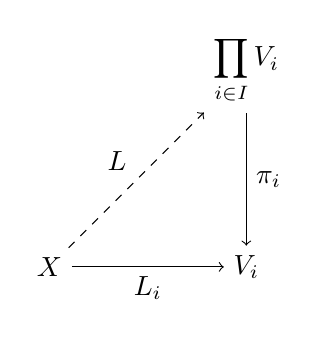
\begin{tikzpicture}[node distance=2.5cm, auto]
	\node (P) {$\displaystyle\prod_{i \in I} \bm{V_i}$};
	\node (Ci) [below of=P] {$\bm{V_i}$};
	\node (X) [left of=Ci] {$\bm X$};
	\draw[->] (X) to node [swap] {$L_i$} (Ci);
	\draw[->, dashed] (X) to node {$L$} (P);
	\draw[->] (P) to node {$\pi_i$} (Ci);
\end{tikzpicture}
\end{figure}
\end{prop}
\begin{proof}
Defina a função
	\begin{align*}
	\func{L}{X}{\prod_{i \in I} V_i}{x}{(L_i(x))_{i \in I}}.
	\end{align*}
Da propriedade universal para conjuntos, $L$ é a única função de $X$ para $\bigtimes_{i \in I} \bm{V_i}$ tal que, para todo $i \in I$, $\pi_i \circ L = L_i$. Falta mostrar que $L$ é função linear. Sejam $c \in C$ e $x_1,x_2 \in V$. Então
	\begin{align*}
	L(x_1+cx_2) &= (L_i(x_1+cx_2))_{i \in I} \\
		&= (L_i(x_1)+cL_i(x_2))_{i \in I} \\
		&= (L_i(x_1))_{i \in I}+c(L_i(x_2))_{i \in I} \\
		&= L(x_1)+cL(x_2). \qedhere
	\end{align*}
\end{proof}

\subsection{Coproduto (Soma)}

\begin{defi}
Seja $(\bm{V_i})_{i \in I} = ((V_i,+_i,\cdot_i))_{i \in I}$ uma família de espaços vetoriais. A \emph{soma categórica} de $(\bm{V_i})_{i \in I}$ é
	\begin{equation*}
	\coprod_{i \in I} \bm{V_i} = (V,+,\cdot),
	\end{equation*}
em que
	\begin{equation*}
	V = \set{v=(v_i)_{i \in I} \in \prod_{i \in I} V_i}{\card{\supp(v)} < \card{\N}},
	\end{equation*}
	\begin{align*}
	\func{+}{V \times V}{V}{(v,v')}{(v_i +_i {v'}_i)_{i \in I}}
	\end{align*}
e
	\begin{align*}
	\func{\cdot}{C \times V}{V}{(c,v)}{(cv_i)_{i \in I}.}
	\end{align*}
\end{defi}

Observe que, se $\card{I} < \card{\N}$, então $\prod_{i \in I} \bm{V_i} = \coprod_{i \in I} \bm{V_i}$.

\begin{prop}[Propriedade Universal]
Sejam $(\bm{V_i})_{i \in I}$ uma família de espaços vetoriais sobre um corpo $\bm C$, $\bm X$ um espaço vetorial sobre $\bm C$ e, para todo $i \in I$, $L_i: \bm{V_i} \to \bm X$ uma função linear. Então existe única função linear $L: \bm X \to \coprod_{i \in I} \bm{V_i}$ tal que, para todo $i \in I$, $L \circ \iota_i = L_i$ (o diagrama comuta).
\begin{figure}
\centering
\begin{tikzpicture}[node distance=2.5cm, auto]
	\node (Ci) {$\bm{V_i}$};
	\node (S) [below of=Ci] {$\displaystyle\coprod_{i \in I} \bm{V_i}$};
	\node (X) [right of=Ci] {$\bm X$};
	\draw[->] (Ci) to node {$L_i$} (X);
	\draw[->, dashed] (S) to node [swap] {$L$} (X);
	\draw[->] (Ci) to node [swap] {$\iota_i$} (S);
\end{tikzpicture}
\end{figure}
\end{prop}

O coproduto de espaços vetoriais é também chamado de \emph{soma} ou \emph{soma direta} e denotado
	\begin{equation*}
	\bigoplus_{i \in I} \bm{V_i}.
	\end{equation*}

%\cleardoublepage
%\section{Notas de Espaços Vetoriais Complexos}

%$(\C^m,i)$, sendo $i \cdot z:= (\sqrt{-1}z_1,\dots,\sqrt{-1}z_m)$.

%\begin{defi}
%Uma \emph{estrutura complexa} em $\R^{2m}$ é um mapa linear $j: \R^{2m} \to \R^{2m}$ que satisfaz
%	\begin{equation*}
%	j \circ j (v) = -v.
%	\end{equation*}
%\end{defi}
%
%Vamos definir uma ação de $\C$ em $\R^{2m}$.
%	\begin{equation*}
%	p(a+\sqrt{-1}b)(v) = av+bj(v).
%	\end{equation*}
%
%\begin{prop}
%$(\R^{2m},j) \simeq (\C^m,i)$.
%\end{prop}
%
%Para cada produto interno, temos um ângulo reto, logo uma multiplicação por $j$ distinta.
%
%Pode-se definir a partir de um vetor normal $n_p$ a um plano tangente em $p$ um mapa linear
%	\begin{equation*}
%	j_p(v) := v \times n_p
%	\end{equation*}
%que satisfaz ${j_p}^2 (v) = -v$.




\section{Projeções Lineares}

\begin{defi}
Seja $\bm V$ um espaço linear sobre um corpo $\bm C$. Uma \emph{projeção linear} em $\bm V$ é uma função linear $p\colon V \to V$ idenpotente: $p^2=p$.
\end{defi}

\begin{prop}
Sejam $\bm V$ um espaço linear sobre um corpo $\bm C$ e $p\colon V \to V$ uma projeção linear.
	\begin{enumerate}
	\item $p|_{p(V)} = \Id|_{p(V)}$;
	
	\item $(\Id-p) \colon V \to V$ é uma projeção linear em $\bm V$;
	
	\item $(\Id-p)\inv(0) = p(V)$ e $(\Id-p)(V) = p\inv(0)$;
	
	\item $V = p(V) \oplus p\inv(0) = p(V) \oplus (\Id-p)(V)$;
	
	\item Para todo $\lambda \in C \setminus \{0,1\}$,
		\begin{equation*}
		(\lambda\Id-p)\inv = \frac{1}{\lambda}\Id + \frac{1}{\lambda(1-\lambda)}p
		\end{equation*}
portanto $\Esp(p) \subseteq \{0,1\}$;

	\item $p$ é invertível se, e somente se, $p=\Id$.

	\item Se $p \neq 0$, seu polinômio mínimo é $x^2-x = x(x-1)$, logo $p$ é diagonalizável pois tem raízes distintas.
	\end{enumerate}
\end{prop}
\begin{proof}
	\begin{enumerate}	
	\item Seja $v \in p(V)$. Então existe $v' \in V$ tal que $v=p(v')$, logo
		\begin{equation*}
		p(v) = p(p(v')) = p^2(v') = p(v') = v.
		\end{equation*}
	
	\item A função $\Id-p$ é linear pois é uma diferença de funções lineares. Basta mostrar que ela é idempotente. Basta notar que% Para todo $v \in V$,
%		\begin{align*}
%		(\Id-p)^2(v) &= (\Id-p)(v-p(v)) \\
%			&= \Id(v-p(v)) - p(v-p(v)) \\
%			&= v-p(v)-p(v)+p^2(v) \\
%			&= v-p(v)-p(v)+p(v)\\
%			&= v-p(v)\\
%			&= (\Id-p)(v)
%		\end{align*}
%o que implica que $(\Id-p)^2 = \Id-p$.
		\begin{equation*}
		(\Id-p)^2 = \Id-p-p+p^2 = \Id-p-p+p = \Id-p.
		\end{equation*}
% INTERESSANTE poder multiplicar funções lineares assim, como se fosse a distributividade de multiplicação e adição. Provar isso generalizando depois.
	
	\item Seja $v \in (\Id-p)\inv(0)$. Então $(\Id-p)(v)=0$, logo $v=p(v)$, o que implica que $v \in p(V)$. Reciprocamente, seja $v \in p(V)$. Então do item 1 segue que $p(v) = v$, logo $(\Id-p)(v) = v-p(v) = v-v = 0$.

A outra relação segue de $(\Id-p)$ ser projeção e $p = \Id - (\Id-p)$.

	\item Seja $v \in p(V) \cap p\inv(0)$. Então $p(v)=0$ e $p(v)=v$, o que implica que $v = p(v) = 0$. Assim temos que $p(V) \cap p\inv(0) = \{0\}$.
%Sejam $v in p(V)$ e $v' \in p\inv(0)$ e $c,c' \in C$ tais que $cv+c'v'=0$. Então
%		\begin{equation*}
%		0 = p(0) = p(cv+c'v') = cp(v)+c'p(v') = cv
%		\end{equation*}
%logo $c=0$, portanto $0 = cv+c'v'=c'v'$, o que implica que $c'=0$.
	
	Seja $v \in V$. Então $p(v) \in p(V)$ e $(\Id-p)(v) \in p\inv(0)$ (pois $(\Id-p)(V) = p\inv(0)$), logo $v = p(v) + (\Id-p)(v)$, o que mostra que $V = p(V) + p\inv(V)$.
	
	\item Note que
		\begin{equation*}
		\frac{1}{1-\lambda} - \frac{1}{\lambda} - \frac{1}{\lambda(1-\lambda)} = \frac{\lambda - (\lambda - 1) - 1}{\lambda(1-\lambda)} = 0,
		\end{equation*}
logo
		\begin{align*}
		(\lambda\Id - p) \circ \left( \frac{1}{\lambda}\Id + \frac{1}{\lambda(1-\lambda)}p \right) &= \Id + \frac{1}{1-\lambda}p - \frac{1}{\lambda}p - \frac{1}{\lambda(1-\lambda)}p^2 \\
%			&= \Id + \frac{1}{1-\lambda}p - \frac{1}{\lambda}p - \frac{1}{\lambda(1-\lambda)}p \\
			&= \Id + \left( \frac{1}{1-\lambda} - \frac{1}{\lambda} - \frac{1}{\lambda(1-\lambda)} \right) p \\
			&= \Id.
		\end{align*}
e
	\begin{equation*}
	\left( \frac{1}{\lambda}\Id + \frac{1}{\lambda(1-\lambda)}p \right) \circ (\lambda\Id - p) = \Id - \frac{1}{\lambda}p + \frac{1}{1-\lambda}p - \frac{1}{\lambda(1-\lambda)}p^2 = \Id.
	\end{equation*}
	
	\item Se $p$ é invertível, $V=p(V)$, logo
		\begin{equation*}
		p = p|_{V} = p|_{p(V)} = \Id|_{p(V)} = \Id|_V = \Id.
		\end{equation*}
A recíproca é evidente.

	\item Evidente.
	
	\end{enumerate}
\end{proof}




%\chapter{Álgebra Multilinear}

\section{Funções Multilineares}

\begin{defi}
Sejam $\bm{V_0},\cdots,\bm{V_{k-1}}$ e $\bm W$ espaços lineares sobre um corpo $\bm C$ e $k \in \N$. Uma função \emph{$k$-linear} de $(\bm{V_0},\ldots,\bm{V_{k-1}})$ para $\bm W$ é uma função
	\begin{equation*}
	L\colon V_0 \times \cdots \times V_{k-1} \to W
	\end{equation*}
qua satisfaz
	\begin{enumerate}
	\item (Multilinearidade) Para todos $i \in [k]$ e
	\begin{equation*}
	(v_0,\ldots,v_{i-1},v_{i+1},\ldots,v_{k-1}) \in V_0 \times \cdots \times V_{i-1} \times V_{i+1} \times \cdots \times V_{k-1},
	\end{equation*}
a função
	\begin{align*}
	\func{L(v_0,\ldots,v_{i-1},\var,v_{i+1},\ldots,v_{k-1})}{\bm{V_i}}{\bm W}{v}{L(v_0,\ldots,v_{i-1},v,v_{i+1},\ldots,v_{k-1})}
	\end{align*}
%	\begin{align*}
%	\func{L(\bm v_0,\ldots,\underbrace{\var}_i,\ldots,\bm v_{k-1})}{\bm{V_i}}{\bm W}{\bm v}{L(\bm v_0,\ldots,\underbrace{\bm v}_i,\ldots,\bm v_{k-1})}
%	\end{align*}
é uma função linear.
	\end{enumerate}
O conjunto dessas funções é denotado
	\begin{equation*}
	\lin(V_0,\ldots,V_{k-1};W)
	\end{equation*}
e, quando todos os espaços $\bm{V_i}$ são iguais, denota-se
	\begin{equation*}
	\lin^k(V,W) := \lin(\underbrace{V,\ldots,V}_k;W)
	\end{equation*}
\end{defi}

\begin{prop}
Sejam $\bm{V_0},\cdots,\bm{V_{k-1}}$ e $\bm W$ espaços lineares sobre um corpo $\bm C$ e, para cada $i \in [k]$, $d_i \in \N$ a dimensão e $b^{(i)}=(b^{(i)}_j)_{j \in [d_i]}$ uma base ordenada de $\bm{V_i}$. Toda função $k$-linear $L \in \lin(V_0,\ldots,V_{k-1};W)$ está determinada pelos seus valores em $(b^{(0)}_{j_0},\ldots,b^{(k-1)}_{j_{k-1}})_{(j_0,\ldots,j_{k-1}) \in [d_0] \times \cdots \times [d_{k-1}]}$.
\end{prop}
\begin{proof}
Sejam $v_0,\ldots,v_{m-1} \in V_k$, $c^0,\ldots,c^{m-1} \in C$, e, para todo $i \in [k]\setminus \{k\}$, $v'_i \in V_i$. Como consequência da propriedade de linearidade generalizada para funções lineares,
	\begin{equation*}
	L\left(v'_0,\ldots,\sum_{i \in [m]} c^i v_i,\ldots,v'_{k-1} \right) = \sum_{i \in [m]} c^i L\left(v'_0,\ldots,v_i,\ldots,v'_{k-1} \right).
	\end{equation*}
Sendo assim, para cada $i \in [k]$, sejam $v_i \in V_i$ e $v_{(i)}^0,\ldots,v_{(i)}^{d_i} \in C$ os coeficientes de $v_i$ na base $b^{(i)}$, de modo que
	\begin{equation*}
	v_i = \sum_{j \in [d_i]} v_{(i)}^j b^{(i)}_j.
	\end{equation*}
Pela linearidade em cada entrada, temos que
	\begin{align*}
	L(v_0,\ldots,v_{k-1}) &= L\left(\sum_{j_0 \in [d_0]} v_{(0)}^{j_0}b^{(0)}_{j_0},\ldots,\sum_{j_{k-1} \in [d_{k-1}]} v_{(k-1)}^{j_{k-1}} b^{(k-1)}_{j_{k-1}} \right) \\
		&= \sum_{j_0 \in [d_0]} v_{(0)}^{j_0} L\left(b^{(0)}_{j_0},\ldots,\sum_{j_{k-1} \in [d_{k-1}]} v_{(k-1)}^{j_{k-1}} b^{(k-1)}_{j_{k-1}} \right) \\
		&\ \, \vdots\qquad\qquad\qquad\qquad\qquad \vdots \\
		&= \sum_{j_0 \in [d_0]} \cdots \sum_{j_{k-1} \in [d_{k-1}]} v_{(0)}^{j_0} \cdots v_{(k-1)}^{j_{k-1}} L\left(b^{(0)}_{j_0},\ldots,b^{(k-1)}_{j_{k-1}} \right) \\
		&= \sum_{(j_0,\ldots,j_{k-1}) \in [d_0] \times \cdots \times [d_{k-1}]} v_{(0)}^{j_0} \cdots v_{(k-1)}^{j_{k-1}} L\left(b^{(0)}_{j_0},\ldots,b^{(k-1)}_{j_{k-1}} \right).
	\end{align*}
%			&= \sum_{\substack{j_0 \in [d_0] \\ \cdots\\ j_{k-1} \in [d_{k-1}]}} v_{0,j_0} \cdots v_{k-1,j_{k-1}} L\left(b_{0,j_0},\ldots,b_{k-1,j_{k-1}} \right).
Portanto a função $L$ está determinada pelos valores que tem nos elementos
	\begin{equation*}
	(b^{(0)}_{j_0},\ldots,b^{(k-1)}_{j_{k-1}})_{(j_0,\ldots,j_{k-1}) \in [d_0] \times \cdots \times [d_{k-1}]}.
	\end{equation*}
%Como há $d_0 \cdots d_{k-1}$ desses elementos, há essa quantidade de escolhas a serem determinadas para se determinarem os valores de $L$.
\end{proof}

\begin{prop}
Sejam $\bm{V_0},\cdots,\bm{V_{k-1}}$ e $\bm W$ espaços lineares sobre um corpo $\bm C$. Então
	\begin{equation*}
	\lin(\bm{V_0},\ldots,\bm{V_{k-1}};\bm W) := (\lin(V_0,\ldots,V_{k-1};W),+,\cdot),
	\end{equation*}	
em que $+$ e $\cdot$ são a soma e o produto escalar pontuais induzidos por $\bm W$, é um espaço linear sobre $\bm C$.
\end{prop}

%Mostrar isomorfismo
%	\begin{align*}
%	\func{\Omega}{\lin^2(V_0,V_1;W)}{\lin(V_0,\lin(V_1,W))}{L}{L(v_0,\var)}.
%	\end{align*}

\subsection{Simetria, Antissimetria e Alternância}

\begin{defi}
Sejam $\bm V$ e $\bm W$ espaços lineares sobre um corpo $\bm C$. Uma função $k$-linear de $\bm V$ para $\bm W$
\begin{enumerate}
	\item \emph{simétrica} é uma função $f \in \lin^k(\bm V,\bm W)$ tal que, para toda permutação $p \in \sime_k$ e todos $v_0$, $\ldots$, $v_{k-1} \in V$,
	\begin{equation*}
	f(v_{p(0)},\ldots,v_{p(k-1)}) = f(v_0,\ldots,v_{k-1});
	\end{equation*}
O conjunto das funções $k$-lineares simétricas é denotado $\mathcal S^k(\bm V,\bm W)$.
	\item \emph{antissimétrica} é uma função $f \in \lin^k(\bm V,\bm W)$ tal que, para toda permutação $p \in \sime_k$ e todos $v_0,\ldots,v_{k-1} \in V$,
	\begin{equation*}
	f(v_{p(0)},\ldots,v_{p(k-1)}) = \prd(p) f(v_0,\ldots,v_{k-1});
	\end{equation*}
	\item \emph{alternada} é uma função $f \in \lin^k(\bm V,\bm W)$ tal que, para todos $v_0,\ldots,v_{k-1} \in V$ linearmente dependentes,
	\begin{equation*}
	f(v_0,\ldots,v_{k-1}) = 0.
	\end{equation*}
O conjunto das funções $k$-lineares alternadas é denotado $\mathcal A^k(\bm V,\bm W)$.
\end{enumerate}
\end{defi}

\begin{prop}
Sejam $\bm V$ e $\bm W$ espaços lineares sobre um corpo $\bm C$ e $f \in \lin^k(\bm V,\bm W)$.
	\begin{enumerate}
	\item A função $f$ é alternada se, e somente se, para todos $v_0$, $\ldots$, $v_{k-1} \in V$ tais que existem $i,j \in [k]$ distintos satizfazendo $v_i = v_j$,
	\begin{equation*}
	f(v_0,\ldots,v_{k-1})=0.
	\end{equation*} 
	\item Se $f$ é alternada, então é antissimétrica. Se $\car(\bm C) \neq 2$ e $f$ é antissimétrica, então é alternada.
	\item Se $\car(\bm C) = 2$, então $f$ é antissimétrica se, e somente se, é simétrica.
	\end{enumerate}
\end{prop}
\begin{proof}
	\begin{enumerate}
	\item Se $f$ é alternada, então, para todos $v_0,\ldots,v_{k-1} \in V$ tais que $v_i = v_j$ para dois $i,j \in [k]$ distintos, o conjunto $\{v_0,\ldots,v_{k-1}\}$ é linearmente dependente, portanto $f(v_0,\ldots,v_{k-1})=0$. Reciprocamente, suponha que $f$ satisfaz a propriedade e sejam $v_0,\ldots,v_{k-1} \in V$ linearmente dependentes. Então existe $i \in [k]$ tal que $v_i$ é combinação linear dos outros $v_j$: existem $c_j \in C$, com $j \in [k]\setminus\{i\}$, tais que
	\begin{equation*}
	v_i = \sum_{j \in [k]\setminus\{i\}} c_j v_j.
	\end{equation*}
Assim, segue da $k$-linearidade e da propriedade enunciada que
	\begin{align*}
	f(v_0,\ldots,v_{k-1}) &= f\left(v_0,\ldots, \sum_{j \in [k]\setminus\{i\}} c_j v_j,\ldots,v_{k-1}\right) \\
		&= \sum_{j \in [k]\setminus\{i\}} c_j f(v_0,\ldots,v_j,\ldots,v_{k-1}) \\
		&=\sum_{j \in [k]\setminus\{i\}} c_j 0 = 0.
	\end{align*}

	\item Suponha $f$ alternada e sejam $v_0,\ldots,v_{k-1} \in V$. Então segue da $k$-linearidade e da alternância de $f$ que
	\begin{align*}
	0 =&f(v_0,\ldots,v_i+v_j,\ldots,v_i+v_j,\ldots,v_{k-1}) \\
		=& f(v_0,\ldots,v_i,\ldots,v_i,\ldots,v_{k-1}) + f(v_0,\ldots,v_i,\ldots,v_j,\ldots,v_{k-1}) \\
		&+f(v_0,\ldots,v_j,\ldots,v_i,\ldots,v_{k-1}) + f(v_0,\ldots,v_j,\ldots,v_j,\ldots,v_{k-1}) \\
		=& f(v_0,\ldots,v_i,\ldots,v_j,\ldots,v_{k-1}) +f(v_0,\ldots,v_j,\ldots,v_i,\ldots,v_{k-1}),
	\end{align*}
portanto
	\begin{equation*}
	f(v_0,\ldots,v_i,\ldots,v_j,\ldots,v_{k-1}) = - f(v_0,\ldots,v_j,\ldots,v_i,\ldots,v_{k-1}).
	\end{equation*}
Como toda permutação $p \in \sime_k$ é um produto de $N \in \N$ inversões, e como $\prd(p)=(-1)^N$, segue por indução que, para toda permutação $p \in \sime_k$,
	\begin{equation*}
	f(v_{p(0)},\ldots,v_{p(k-1)}) =(-1)^N f(v_0,\ldots,v_{k-1}) = \prd(p) f(v_0,\ldots,v_{k-1}).
	\end{equation*}

Suponha que $\car(\bm C) \neq 2$. Sejam $f \in \lin^k(\bm V,\bm W)$ antissimétrica e $v_0$, $\ldots$, $v_{k-1} \in V$ tais que $v_i = v_j$ para dois $i,j \in [k]$ distintos. Considerando a permutação $(i \quad j) \in \sime_k$, segue da antissimetria de $f$ e de $\prd((i \quad j))=-1$ que
	\begin{align*}
	f(v_0,\ldots,v_i,\ldots,v_j,\ldots,v_{k-1}) &= f(v_0,\ldots,v_j,\ldots,v_i,\ldots,v_{k-1}) \\
		&= - f(v_0,\ldots,v_i,\ldots,v_j,\ldots,v_{k-1}),
	\end{align*}
portanto
	\begin{equation*}
	2 f(v_0,\ldots,v_{k-1})=0.
	\end{equation*}
Como $\car(\bm C) \neq 2$, segue que $f(v_0,\ldots,v_{k-1})=0$. Do item 1 segue que $f$ é alternada.

\item Se $\car(\bm C) = 2$, então $-1=1$. Isso implica que, para qualquer permutação $p$, $\prd(p)=1$.
\end{enumerate}
\end{proof}

Um exemplo de uma função multilinear que é antissimétrica mas não é alternada em para um corpo de característica $2$ é o seguinte. Seja $\Z_2=\{0,1\}$ o corpo de característica $2$ e considere a função $f\colon \Z_2 \times \Z_2 \to \Z_2$ dada por
	\begin{align*}
	\func{f}{\Z_2 \times \Z_2}{\Z_2}{(0,0)}{0 \\
															(0,1) &\mapsto 0 \\
															(1,0) &\mapsto 0 \\
															(1,1) &\mapsto 1												
														}
	\end{align*}
Pode-se verificar que essa função é bilinear e antissimétrica, mas não é alternada porque $f(1,1)=1 \neq 0$.

De modo mais geral, para qualquer função $p\colon [k] \to [k]$, não necessariamente bijetiva, considerando o caráter $\prd(p)$ que vale $0$ se $p$ não é uma permutação, e $1$ ou $-1$ conforme a paridade da permutação $p$, as definições de formas antissimétricas e alternadas podem ser unificadas: a de formas antissimétricas pode ser mantida como foi feita e, para o caso de formas alternadas, devido à propriedade 1 da proposição anterior, pode-se enunciar: para qualquer $p\colon [k] \to [k]$,
	\begin{equation*}
	f(v_{p(0)},\ldots,v_{v_{k-1}}) = \prd(p) f(v_0,\ldots,v_{k-1}).
	\end{equation*}
O caso em que $p$ é bijetiva recai na definição de formas antissimétricas, e o caso em que $p$ não é bijetiva recai na definição de formas alternadas, mais precisamente da propriedade 1 da proposição anterior, que é equivalente à definição de forma alternada.

\begin{prop}
Sejam $\bm V$ e $\bm W$ espaços lineares sobre um corpo $\bm C$. Os espaços $\mathcal S^k(\bm V,\bm W)$ e $\mathcal A^k(\bm V,\bm W)$ são subespaços lineares de $\lin^k(\bm V,\bm W)$.
\end{prop}

\section{Formas Multilineares}

\begin{defi}
Seja $\bm V$ um espaço linear sobre um corpo $\bm C$. Uma \emph{forma $k$-linear} em $\bm V$ é uma função $f \in \lin^k(\bm V;\bm C)$, ou seja, um funcional $k$-linear em $(\bm V,\ldots,\bm V)$. O conjunto das formas $k$-lineares simétricas é denotado $\mathcal{S}^k(\bm V)$ e o das alternadas é denotado $\mathcal{A}^k(\bm V)$.
\end{defi}

Temos que $\mathcal{S}^1(\bm V) = \mathcal{A}^1(\bm V) = \lin^k(\bm V)$ e $\mathcal{S}^0(\bm V) = \mathcal{A}^0(\bm V) = \lin^0(\bm V) = C$.

\subsection{Produto Tensorial de Formas Multilineares}

\begin{defi}
Sejam $\bm V$ um espaço linear sobre um corpo $\bm C$, $f \in \lin^k(V)$, $f' \in \lin^{k'}(V)$ e $v_0,\ldots,v_{k+k'-1} \in V$. O \emph{produto tensorial} de $f$ e $f'$ em $(v_0,\ldots,v_{k+k'-1})$ é
	\begin{equation*}
	(f \otimes f')(v_0,\ldots,v_{k+k'-1}) := f(v_0,\ldots,v_{k-1})f'(v_k,\ldots,v_{k+k'-1}).
	\end{equation*}
Sejam $n \in \N$ e $(f_i)_{i \in [n]}$ formas multilineares em $\bm V$. O \emph{produto tensorial} dessas formas é definido recursivamente
	\begin{equation*}
	\bigotimes_{i \in [n]} f_i := \begin{cases}
		f_0,& n=1 \\
		\left(\displaystyle\bigotimes_{i \in [n-1]} f_i \right) \otimes f_{n-1} ,& n>1.
	\end{cases}
	\end{equation*}
\end{defi}

\begin{prop}
Seja $\bm V$ um espaço linear sobre um corpo $\bm C$.
	\begin{enumerate}
	\item Para todas formas $f \in \lin^k(\bm V)$ e $f' \in \lin^{k'}(\bm V)$, a função $f \otimes f'$ é uma forma $k+k'$-linear.
	\item (Bilinearidade) A função
		\begin{align*}
		\func{\otimes}{\lin^k(\bm V) \times \lin^{k'}(\bm V)}{\lin^{k+k'}(\bm V)}{(f,f')}{f \otimes f'}
		\end{align*}
é bilinear.
	\item (Associatividade) Para todas formas $f \in \lin^k(\bm V)$, $f' \in \lin^{k'}(\bm V)$ e $f'' \in \lin^{k''}(\bm V)$,
		\begin{equation*}
		(f \otimes f') \otimes f'' = f \otimes (f' \otimes f'').
		\end{equation*}
	\end{enumerate}
\end{prop}

\subsection{Produto Alternado de Formas Multilineares}

\begin{defi}
Sejam $\bm V$ um espaço linear sobre um corpo $\bm C$, $f \in \mathcal{A}^k(\bm V)$, $f' \in \mathcal{A}^{k'}(\bm V)$ e $v_0,\ldots,v_{k+k'-1} \in \bm V$. O \emph{produto alternado} (ou \emph{exterior}) de $f$ e $f'$ em $(v_0,\ldots,v_{k+k'-1})$ é
%	\begin{equation*}
%	(f \wedge f')(v_0,\ldots,v_{k+k'-1}) := \frac{1}{k!k'!} \sum_{p \in \sime_{k+k'}} \prd(p) f(v_{p(0)},\ldots,v_{p(k-1)})f'(v_{p(k)},\ldots,v_{p(k+k'-1)}).
%	\end{equation*}
	\begin{equation*}
	(f \wedge f')(v_0,\ldots,v_{k+k'-1}) := \frac{1}{k!k'!} \sum_{p \in \sime_{k+k'}} \prd(p) (f \otimes f')(v_{p(i)})_{i \in [k+k']}.
	\end{equation*}
Sejam $n \in \N$ e $(f_i)_{i \in [n]}$ formas multilineares em $\bm V$. O \emph{produto alternado} dessas formas é definido recursivamente
	\begin{equation*}
	\bigwedge_{i \in [n]} f_i := \begin{cases}
		f_0,& n=1 \\
		\left(\displaystyle\bigwedge_{i \in [n-1]} f_i \right) \wedge f_{n-1} ,& n>1.
	\end{cases}
	\end{equation*}
\end{defi}

\begin{prop}
Seja $\bm V$ um espaço linear sobre um corpo $\bm C$.
	\begin{enumerate}
	\item Para todas formas $f \in \lin^k(\bm V)$ e $f' \in \lin^{k'}(\bm V)$, a função $f \wedge f'$ é uma forma $k+k'$-linear alternada.
	\item (Bilinearidade) A função
		\begin{align*}
		\func{\wedge}{\mathcal{A}^k(\bm V) \times \mathcal{A}^{k'}(\bm V)}{\mathcal{A}^{k+k'}(\bm V)}{(f,f')}{f \wedge f'}
		\end{align*}
é bilinear.
	\item (Associatividade) Para todas formas alternadas $f \in \mathcal{A}^k(\bm V)$, $f' \in \mathcal{A}^{k'}(\bm V)$ e $f'' \in \mathcal{A}^{k''}(\bm V)$,
		\begin{equation*}
		(f \wedge f') \wedge f'' = f \wedge (f' \wedge f'').
		\end{equation*}
	\item	 Para todas formas $f \in \mathcal{A}^k(\bm V)$ e $f' \in \mathcal{A}^{k'}(\bm V)$
		\begin{equation*}
		f' \wedge f = (-1)^{kk'} f \wedge f'.
		\end{equation*}
	\end{enumerate}
\end{prop}
\begin{proof}
	\begin{enumerate}
	\item Seja $v_0,\ldots,v_{k+k'-1} \in V$ e $\bar p \in \sime_{k+k'}$. Então
		\begin{align*}
		(f \wedge f') (v_{\bar p(i)})_{i \in [k+k']} &= \frac{1}{k!k'!} \sum_{p \in \sime_{k+k'}} \prd(p) (f \otimes f')(v_{p(\bar p(i))})_{i \in [k+k']} \\
			&= \frac{1}{k!k'!} \sum_{p \in \sime_{k+k'}} \prd(\bar p\inv p) (f \otimes f')(v_{p(i)})_{i \in [k+k']} \\
			&= \frac{1}{k!k'!} \sum_{p \in \sime_{k+k'}} \prd(\bar p\inv)\prd(p) (f \otimes f')(v_{p(i)})_{i \in [k+k']} \\
			&= \prd(\bar p\inv)\frac{1}{k!k'!} \sum_{p \in \sime_{k+k'}} \prd(p) (f \otimes f')(v_{p(i)})_{i \in [k+k']} \\
			&= \prd(\bar p)(f \wedge f')(v_i)_{i \in [k+k']}.
		\end{align*}
	\item	 
	\end{enumerate}
\end{proof}

%Isso definine uma função bilinear
%	\begin{align*}
%	\func{\wedge}{\mathcal{A}^k(\bm V) \times \mathcal{A}^l(\bm V)}{\mathcal{A}^{k+l}(\bm V)}{(f,g)}{f \wedge g}
%	\end{align*}

%Esse produto é uma forma $\sum_{i \in [n]} k_i$-linear em $\bm V$.

%\begin{defi}
%Sejam $\bm V$ um espaço linear de dimensão finita $d$ sobre um corpo $\bm C$, $(b_i)_{i \in [d]}$ um base ordenada de $\bm V$ e $({b_i}^*)_{i \in [d]}$ a base dual de $\bm{V^*}$. Para todo subconjunto $I \subseteq [d]$, e $(i_j)_{j \in [\card{I}]}$ a indexação crescente de $I$ ($i_0 < \cdots < i_{\card{I}-1}$), define-se
%	\begin{equation*}
%	\bigwedge_{i \in I} b_i^* := b_{i_0}^* \wedge \cdots \wedge b_{i_{k-1}}^*.
%	\end{equation*}
%\end{defi}

\begin{prop}
Sejam $\bm V$ um espaço linear de dimensão finita $d$ sobre um corpo $\bm C$, $(b_i)_{i \in [d]}$ um base ordenada de $\bm V$ e $({b_i}^*)_{i \in [d]}$ a base dual de $\bm{V^*}$. Então $\mathcal{A}^k(\bm V)$ é um espaço linear sobre $\bm C$ de dimensão $\binom{d}{k}$ e o conjunto
	\begin{equation*}
	\set{b_{i_0}^* \wedge \cdots \wedge b_{i_{k-1}}^*}{i_0 < \cdots < i_{k-1} \in [d]}
	\end{equation*}
%	\begin{equation*}
%	\set{\bigwedge_{i \in I} b_{i}^*}{I \subseteq [d], \card{I}=k}
%	\end{equation*}
de formas alternadas $k$-lineares em $\bm V$ é uma base para $\mathcal{A}^k(\bm V)$.
\end{prop}

Em particular, isso mostra que formas $d$-lineares num espaço de dimensão $d$ são todas múltiplos umas das outras, pois $\binom{d}{d}=1$. Podemos fixar o valor de uma das formas como 1 na base canônica e chamá-la de \emph{determinante}.

\begin{defi}
Seja $d \in \N$. O \emph{determinante} em $\R^d$ é a forma $d$-linear
	\begin{equation*}
	\det := {e_0}\dual \wedge \ldots \wedge {e_{d-1}}\dual.
	\end{equation*}
%Sejam $\bm V$ um espaço linear de dimensão finita $d$ sobre um corpo $\bm C$ e $b=(b_i)_{i \in [d]}$ uma base de $\bm V$. O \emph{determinante} em $\bm V$ com respeito a $b$ é a forma $d$-linear
%	\begin{equation*}
%	\det\nolimits_{b} := {b_0}\dual \wedge \ldots \wedge {b_{d-1}}\dual.
%	\end{equation*}
%No caso de $V = \R^d$, o determinante é definido com respeito à base canônica
%	\begin{equation*}
%	\det := {e_0}\dual \wedge \ldots \wedge {e_{d-1}}\dual.
%	\end{equation*}
\end{defi}

Como comentado, essa é a única forma $d$-linear em $\R^d$ tal que	\begin{equation*}
	\det(e_0,\ldots,e_{d-1})=1.
	\end{equation*}

Na seção seguinte, definiremos o conceito de determinante de modo mais geral e independente de base.

\subsection{Formas Puxadas e Determinante}

\begin{defi}
Sejam $\bm V$ e $\bm V'$ espaços lineares sobre um corpo $\bm C$, $L \colon V \to V'$ uma função linear e $f \in \lin^k(V')$. A \emph{forma $k$-linear puxada} por $L$ de $f$ é a função
	\begin{align*}
	\func{L\dual f}{V^k}{C}{(v_0,\ldots,v_{k-1})}{f(L(v_0),\ldots,L(v_{k-1})).}
	\end{align*}
A função \emph{$k$-adjunta} induzida por $L$ é a função linear
	\begin{align*}
	\func{L\dual}{\lin^k(V')}{\lin^k(V)}{f}{L\dual f.}
	\end{align*}
\end{defi}

A notação é ambígua porque, para cada $k \in [d+1]$, a função $L\dual$ é uma função diferente. De fato, para $f \in \lin^k(V')$,
	\begin{equation*}
	L\dual f = f \circ L^{\otimes k},
	\end{equation*}
o que quer dizer que
	\begin{equation*}
	L \dual = (L^{\otimes k})\pux
	\end{equation*}

\begin{prop}
Sejam $\bm V$, $\bm V'$ e $\bm V''$ espaços lineares sobre um corpo $\bm C$ e $L\colon V \to V'$ e $L'\colon V' \to V''$ funções lineares. Então
	\begin{equation*}
	(L' \circ L)\dual = {L}\dual \circ {L'}\dual.
	\end{equation*}
\end{prop}
\begin{proof} Seja $f \in \lin^k(V)$ tal que $f \neq 0$. Então
	\begin{align*}
	(L' \circ L)\dual f (v_0,\ldots,v_{k-1}) &= f((L' \circ L)(v_0),\ldots,(L' \circ L)(v_{k-1})) \\
		&= f(L'(L(v_0)),\ldots,L'(L(v_{k-1}))) \\
		&= {L'}\dual f(L(v_0),\ldots,L(v_{k-1})) \\
		&= L\dual({L'}\dual f)(v_0,\ldots,v_{k-1}) \\
		&= (L\dual \circ {L'}\dual) f(v_0,\ldots,v_{k-1}).
	\end{align*}
\end{proof}


Essas funções $k$-adjuntas estão também definidas se restringimos os espaços de funcionais $\lin^k$ para espaços de funcionais alternados $\alter^k$. Se considerarmos um espaço linear $d$-dimensional $\bm V$, o espaço $\alter^d(\bm V)$ é um espaço $1$-dimensional, o que implica que todas funções lineares são multiplicações por constantes. Isso nos permite definir o determinante de uma função linear instrinsecamente como a constante de é seu $d$-adjunto.

\begin{defi}
Sejam $\bm V$ um espaço linear $d$-dimensional sobre um um corpo $\bm C$, $L\colon V \to V$ uma função linear e $L\dual\colon \alter^d(V) \to \alter^d(V)$. O \emph{determinante} de $L$ é a constante $\det(L) \in C$ tal que, para todas formas $f \in \alter^d(\bm V)$,
	\begin{equation*}
	L\dual f = \det(L) f.
	\end{equation*}
\end{defi}

Isso nos dá por definição a igualdade
	\begin{equation*}
	f(L(v_0),\ldots,L(v_{d-1})) = \det(L)f(v_0,\ldots,v_{d-1}).
	\end{equation*}

\begin{prop}
Sejam $\bm V$ um espaço linear $d$-dimensional sobre um um corpo $\bm C$ e $L,L' \in \lin(V,V)$. Então
	\begin{equation*}
	\det(L' \circ L) = \det(L)\det(L').
	\end{equation*}
\end{prop}
\begin{proof}
Seja $f \in \alter^n(V)$ tal que $f \neq 0$. Então
	\begin{equation*}
	\det(L' \circ L)f = (L' \circ L)\dual f = ({L}\dual \circ {L'}\dual) f = \det(L)\det(L') f.
	\end{equation*}
\end{proof}

\begin{prop}
Sejam $\bm V$ um espaço linear $d$-dimensional sobre um um corpo $\bm C$ e $L\colon V \to V$ uma função linear. Então $L$ é invertível se, e somente se, $\det(L) \neq 0$.
\end{prop}
\begin{proof}
Basta notar que $L$ é invertível se, e somente se, leva base em base e $f \in \alter^d(V)$ é nula em um conjunto linearmente independente de vetores.
\end{proof}


















\subsection{Extras}

Definimos
	\begin{equation*}
	[d]^{\uparrow k} := \set{(i_0,\ldots,i_{k-1}) \in [d]^k}{i_{0}<\cdots<i_{k-1}}.
	\end{equation*}
Note que
	\begin{equation*}
	\card{[d]^{\uparrow k}} = \card{\binom{[d]}{k}} = \binom{d}{k},
	\end{equation*}
em que $\binom{[d]}{k} = \set{I \subseteq [d]}{\card{I}=k}$.


\cleardoublepage





\section{Produto Tensorial de Espaços Lineares}

\begin{defi}
Sejam $X$ um conjunto, $\bm C$ um corpo e $f: X \to C$ uma função. O \emph{suporte} de $f$ é o conjunto
	\begin{equation*}
	\supp(f) := f\inv\left(\{0\}^\complement\right) = \set{x \in X}{f(x) \neq 0}.
	\end{equation*}
\end{defi}

%\begin{defi}
%Sejam $I$ um conjunto e $\bm C$ um corpo. Uma \emph{combinação linear formal} de elementos de $I$ sobre $\bm C$ é uma função $v: I \to C$ de suporte finito. Definido $c_i := v(i) \in C$, denota-se
%	\begin{equation*}
%	v = \sum_{i \in I} c_i v_i.
%	\end{equation*}
%\end{defi}

\begin{defi} Sejam $I$ um conjunto e $\bm C$ um corpo. O \emph{espaço linear livre em $I$} sobre $\bm C$ é o conjunto 
	\begin{equation*}
	\liv(I) := \set{v \in C^I}{\card{\supp(v)}<\card{\N}}.
	\end{equation*}
Os elementos de $\liv(I)$ são as \emph{combinações lineares formais} de elementos de $I$ sobre $\bm C$.

A \emph{inclusão} de $I$ em $\liv(I)$ é a função
	\begin{align*}
	\func{\iota}{I}{\liv(I)}{v}{
		\begin{aligned}[t]
		\func{\delta_v}{I}{C}{i}{\begin{cases}
							1,& i = v \\
							0,& i \neq v.
						\end{cases}}
		\end{aligned}	
	}
	\end{align*}
Denotaremos os elementos $\delta_v$ por $v$ quando não houver necessidade de diferenciá-los.
\end{defi}

Note que $\liv(I) = \coprod_{i \in I} \bm C$ e, portanto,
	\begin{equation*}
	\bm{\liv(I)} := (\liv(I)),+,\cdot),
	\end{equation*}	
em que $+$ e $\cdot$ são a soma e o produto escalar pontuais induzidos por $\bm W$, é um espaço linear sobre $\bm C$ com base $\set{\delta_v}{v \in I}$. Por isso, definido $c_i := v(i) \in C$, uma função $v: I \to C$ de suporte finito é uma soma
	\begin{equation*}
	v = \sum_{i \in I} c_i \delta_i = \sum_{i \in I} c_i v_i,
	\end{equation*}
que é uma soma finita porque $\supp(v)$ é finito, ou seja, somente uma quantidade finita dos $c_i$ é não nulo.

\begin{prop}[Propriedade Caracterítica dos Espaços Lineares Livres]
Sejam $I$ um conjunto, $\bm C$ um corpo e $\bm V$ um espaço linear sobre $\bm C$. Para toda função $f: I \to V$, existe uma única função linear $\bar f: \liv(I) \to V$ tal que $\bar f \circ \iota = f$ (o diagrama comuta).
\begin{figure}
\centering
\begin{tikzpicture}[node distance=2.5cm, auto]
	\node (F) {$\bm{\liv(I)}$};
	\node (I) [below of=F] {$I$};
	\node (V) [right of=I] {$\bm V$};
	\draw[->] (I) to node [swap] {$f$} (V);
	\draw[->, dashed] (F) to node {$\bar f$} (V);
	\draw[->] (I) to node {$\iota$} (F);
\end{tikzpicture}
\end{figure}
\end{prop}
\begin{proof} Basta usar a propriedade característica de coproduto de espaços lineares, ou notar o que uma função $\bar f$ pode ser construída definindo seus valores em $\delta_v \in \liv(I)$. Para todo $v=\sum_{i \in I} c_i v_i \in \liv(I)$, define-se
	\begin{equation*}
	\bar f\left(\sum_{v_i \in I} c_i v_i\right):= \sum_{v_i \in I} c_i f(v_i)
	\end{equation*}
A função é única pois está definida da base $\delta_v$.
\end{proof}

\begin{defi}
Sejam $\bm C$ um corpo e $V_0,\ldots,V_{n-1}$ conjuntos. Consideremos o conjunto $\mathcal R$ gerado por vetores de $\liv(V_0 \times \cdots \times V_{n-1})$ da forma
	\begin{equation*}
	(v_0,\ldots,v_i+v'_i,\ldots,v_{n-1}) - (v_0,\ldots,v_i,\ldots,v_{n-1}) - (v_0,\ldots,v'_i,\ldots,v_{n-1}),
	\end{equation*}
	\begin{equation*}
	(v_0,\ldots,cv_i,\ldots,v_{n-1}) - c(v_0,\ldots,v_i,\ldots,v_{n-1}),
	\end{equation*}
em que $v_i,v'_i \in V_i$ para todo $i \in [n]$ e $c \in C$. O \emph{produto tensorial} de $V_0,\ldots,V_{n-1}$ é o espaço linear
	\begin{equation*}
	\bm{V_0} \otimes \cdots \otimes \bm{V_{n-1}} := \quo{\liv(\bm{V_0} \times \cdots \times \bm{V_{n-1}})}{\bm{\mathcal R}}
	\end{equation*}
A classe de equivalência de $(v_0,\ldots,v_{n-1}) \in V_0 \times \cdots \times V_{n-1}$ em $V_0 \otimes \cdots \otimes V_{n-1}$ é denotada $v_0 \otimes \cdots \otimes v_{n-1}$ e o \emph{mapa tensorial canônico} é a função $\otimes := \pi \circ \iota\colon V_0 \times \cdots \times V_{n-1} \to  V_0 \otimes \cdots \otimes V_{n-1}$, em que $\pi\colon \liv(V_0 \times \cdots \times V_{n-1}) \to \mathcal R$ é a projeção do quociente de espaços lineares.
\end{defi}

%\begin{defi}
%Sejam $\bm C$ um corpo, $(V_i)_{i \in I}$ uma família de conjuntos e $\bm{\mathcal R}$ o espaço linear gerado pelos vetores de $\liv(\prod_{i \in I} V_i)$ da forma
%	\begin{equation*}
%	(\ldots,cv_i,\ldots) - c(\ldots,v_i,\ldots),
%	\end{equation*}
%	\begin{equation*}
%	(\ldots,v_i+v'_i,\ldots) - (\ldots,v_i,\ldots) - (\ldots,v'_i,\ldots),
%	\end{equation*}
%em que $v_i,v'_i \in V_i$ para todo $i \in I$ e $c \in C$. O \emph{produto tensorial} de $(V_i)_{i \in I}$ é o espaço linear
%	\begin{equation*}
%	\bigotimes_{i \in I} \bm{V_i} := \bm{\quo{\displaystyle\liv\left(\prod_{i \in I} V_i\right)}{\mathcal R}}.
%	\end{equation*}
%A classe de equivalência de $(v_i)_{i \in I} \in \prod_{i \in I} V_i$ em $\bigotimes_{i in I} V_i$ é denotada $\otimes_{i \in I} v_i$. Para $I$ finito, denotamos
%	\begin{equation*}
%	\bigotimes_{i \in I} \bm{V_i} = \bm V_0 \otimes \cdots \otimes V_{n-1}
%	\end{equation*}
%e
%	\begin{equation*}
%	\otimes_{i \in I} v_i = v_0 \otimes \cdots \otimes v_{n-1}.
%	\end{equation*}
%\end{defi}



\begin{prop}[Propriedade Característica de Produto Tensorial]
Sejam $\bm V_0,$ $\ldots,$ $\bm V_{n-1},$ $\bm W$ espaços lineares sobre um corpo $\bm C$.
	\begin{enumerate}
	\item O mapa tensorial canônico
	\begin{equation*}
	\otimes\colon \bm{V_0} \times \cdots \times \bm{V_{n-1}} \to \bm{V_0} \otimes \cdots \otimes \bm{V_{n-1}}
	\end{equation*}
é uma função multilinear.
	\item Para toda função multilinear $L\colon \bm{V_0} \times \cdots \times \bm{V_{n-1}} \to \bm W$, existe única função linear $\bar L\colon \bm{V_0} \otimes \cdots \otimes \bm{V_{n-1}} \to \bm W$ tal que $\bar L \circ \otimes = L$ (o diagrama comuta).
\begin{figure}
\centering
\begin{tikzpicture}[node distance=3cm, auto]
	\node (T) {$\bm{V_0} \otimes \cdots \otimes \bm{V_{n-1}}$};
	\node (I) [below of=T] {$\bm{V_0} \times \cdots \times \bm{V_{n-1}}$};
	\node (V) [right of=I] {$\bm W$};
	\draw[->] (I) to node [swap] {$L$} (V);
	\draw[->, dashed] (T) to node {$\bar L$} (V);
	\draw[->] (I) to node {$\otimes$} (T);
\end{tikzpicture}
\end{figure}
	\end{enumerate}
\end{prop}
\begin{proof}
	\begin{enumerate}
	\item Vale por definição.
	
	\item Pela propriedade característica de espaços lineares livres, existe única função linear $\tilde L: \liv(V_0 \times \cdots \times V_{n-1}) \to W$ tal que $\tilde L \circ \iota = L$. Mas como $L$ é multilinear, o subespaço $\mathcal R$ está contido no núcleo de $\tilde L$, pois, para todos $v_i,v'_i \in V_i$, com $i \in [n]$, e $c \in C$,
	\begin{align*}
	\tilde L(v_0,\ldots,v_i+v'_i,\ldots,v_{n-1}) &= L(v_0,\ldots,v_i+v'_i,\ldots,v_{n-1}) \\
		&=L(v_0,\ldots,v_i,\ldots,v_{n-1}) + L(v_0,\ldots,v'_i,\ldots,v_{n-1}) \\
		&=\tilde L(v_0,\ldots,v_i,\ldots,v_{n-1}) + \tilde L(v_0,\ldots,v'_i,\ldots,v_{n-1}) \\
		&=\tilde L((v_0,\ldots,v_i,\ldots,v_{n-1}) + (v_0,\ldots,v'_i,\ldots,v_{n-1}))
	\end{align*}
e
	\begin{align*}
	\tilde L(v_0,\ldots,cv_i,\ldots,v_{n-1}) &= L(v_0,\ldots,cv_i,\ldots,v_{n-1}) \\
		&=cL(v_0,\ldots,v_i,\ldots,v_{n-1})) \\
		&= c\tilde L(v_0,\ldots,v_i,\ldots,v_{n-1}) \\
		&= \tilde L(c(v_0,\ldots,v_i,\ldots,v_{n-1})).
	\end{align*}
Isso implica que existe função linear $\bar L: V_0 \otimes \cdots \otimes V_{n-1} \to W$ que satisfaz $\bar L \circ \pi = \tilde L$. Como $\otimes = \pi \circ \iota$, segue que
	\begin{equation*}
	\bar L \circ \otimes = \bar L \circ \pi \circ \iota = \tilde L \circ \iota = L.
	\end{equation*}
	\end{enumerate}

\end{proof}

Algumas identidades importantes. Os espaços lineares das funções multilineares é isomorfo ao espaço das funções lineares no produto tensorial:
	\begin{equation*}
	\lin(\bm{V_0},\ldots,\bm{V_{n-1}};\bm W) \simeq \lin(\bm{V_0} \otimes \cdots \otimes \bm{V_{n-1}};\bm W).
	\end{equation*}

%	\begin{equation*}
%	\bm{C^{V_0 \times \cdots \times V_{n-1}}} \simeq \bm{C^{V_0} \otimes \cdots \otimes C^{V_{n-1}}}
%	\end{equation*}




\subsection{Tensores}

\begin{defi}
Seja $\bm V$ um espaço linear sobre um corpo $\bm C$. A $k$-\emph{potência tensorial} de $\bm V$ é o espaço
	\begin{equation*}
	V^{\otimes k} := \bigotimes_{i \in [k]} V = \underbrace{V \otimes \cdots \otimes V}_{k}.
	\end{equation*}
Um $k$-vetor de $\bm V$ é um elemento de $V^{\otimes k}$ e um $k$-covetor de $\bm V$ é um elemento de $(V\dual)^{\otimes k}$.

A \emph{$(p,q)$-potência tensorial} de $\bm V$ é o espaço
	\begin{equation*}
	V^{\otimes (p,q)} := V^{\otimes p} \otimes (V\dual)^{\otimes q}.
	\end{equation*}
%	\begin{equation*}
%	V^{\otimes p*q} := V^{\otimes p} \otimes (V\dual)^{\otimes q}.
%	\end{equation*}
Um $(p,q)$-tensor de $\bm V$ é um elemento de $V^{\otimes (p,q)}$. A \emph{álgebra tensorial} de $\bm V$ é o espaço
	\begin{equation*}
	\bigotimes V := \bigoplus_{(p,q) \in \N \times \N} V^{\otimes (p,q)}.
	\end{equation*}
\end{defi}

Temos as identificações
	\begin{align*}
	V^{\otimes (0,0)} &= C \\
	V^{\otimes (1,0)} &= V \\
	V^{\otimes (0,1)} &= V\dual \\
	V^{\otimes (1,1)} &= \lin(V,V). \\
%	V^{\otimes (p,q)} &= \lin(V^{\otimes q},V^{\otimes p})
	\end{align*}












\chapter{Álgebras sobre Corpos}

\section{Álgebra e Ação Adjunta}

\begin{defi}
Seja $\bm C$ um corpo. Uma \emph{álgebra} sobre $\bm C$ é um par $(\bm A,\cdot)$ em que $\bm A$ é um espaço vetorial sobre $\bm C$ e $\cdot\colon A \times A \to A$ é uma função bilinear. Uma álgebra é \emph{associativa, comutativa} ou \emph{antissimétrica} conforme a respectiva propriedade do produto $\cdot$, e é unitária se $\cdot$ tem identidade.
\end{defi}

\begin{defi}
Sejam $(\bm A,\cdot)$ uma álgebra sobre um corpo $\bm C$ e $a \in A$. A \emph{ação adjunta} em $\bm A$ baseada em $a$ é a função linear
	\begin{align*}
	\func{\adj_a}{A}{A}{a'}{a \cdot a'.}
	\end{align*}
\end{defi}

\begin{prop}
Seja $(\bm A,\cdot)$ uma álgebra sobre um corpo $\bm C$. Então $(\lin(A,A),\circ)$ é uma álgebra associativa sobre $\bm C$.
\end{prop}
\begin{proof}
Sabemos que $\lin(A,A)$ é um espaço linear. Para mostrar que é uma álgebra, devemos mostrar que $\circ$ é bilinear. Sejam $L,L,L'' \in \lin(A,A)$ e $c \in C$. Então, para todo $a \in A$,
	\begin{align*}
	((cL+L') \circ L'')(a) &= (cL+L')(L''(a)) \\
		&= cL(L''(a))+L'(L''(a)) \\
		&= cL \circ L''(a) + L' \circ L''(a) \\
		&= (cL \circ L'' + L' \circ L'')(a).
	\end{align*}
Isso mostra que $(cL+L') \circ L'' = cL \circ L'' + L' \circ L''$. Agora,
	\begin{align*}
	(L \circ (cL'+L''))(a) &= L((cL'+L'')(a)) \\
		&= L(cL'(a)+L''(a)) \\
		&= cL(L'(a))+L(L''(a)) \\
		&= cL \circ L'(a)+L \circ L''(a) \\
		&= (cL \circ L' + L \circ L'')(a).
	\end{align*}
Isso mostra que $L \circ (cL'+L'') = cL \circ L' + L \circ L''$. A composição de funções é associativa, portanto a álgebra é associativa.
\end{proof}

\begin{prop}
Sejam $(\bm A,\cdot)$ uma álgebra sobre um corpo $\bm C$ e $I$ um conjunto. Então $(A^I,\cdot)$, em que $\cdot\colon A^I \times A^I \to A^I$ é o produto entrada a entrada, é uma álgebra sobre $\bm C$. Se o produto de $A$ é associativo ou comutativo, então o produto de $A^I$ é, respectivamente, associativo ou comutativo, e é se $A$ é unitária, $(1)_{in \in I}$ é identidade do produto de $A^I$.
\end{prop}
\begin{proof}
Sabemos que $A^I$ é um espaço linear sobre $\bm C$. Basta mostrar que $\cdot$ é um produto bilinear. Sejam $(a_i)_{i \in I},(a'_i)_{i \in I},(a''_i)_{i \in I} \in A^I$ e $c \in C$. Então
	\begin{align*}
	(c(a_i)_{i \in I} + (a'_i)_{i \in I}) \cdot (a''_i)_{i \in I} &= (ca_i + a'_i)_{i \in I} \cdot (a''_i)_{i \in I} \\
	&= ((ca_i + a'_i) \cdot a''_i)_{i \in I} \\
	&= (ca_i \cdot a''_i + a'_i \cdot a''_i)_{i \in I} \\
	&= c(a_i \cdot a''_i)_{i \in I} + (a'_i \cdot a''_i)_{i \in I} \\
	&= c(a_i)_{i \in I} \cdot (a''_i)_{i \in I} + (a'_i)_{i \in I} \cdot (a''_i)_{i \in I}.
	\end{align*}
A demonstração da linearidade na segunda entrada é análoga, e as demonstrações de associatividade e comutatividade e identidade são triviais.
\end{proof}

\begin{prop}
Seja $(\bm A,\cdot)$ uma álgebra sobre um corpo $\bm C$. A álgebra $\bm A$ é associativa se, e somente se, para todos $a,a' \in A$,
	\begin{equation*}
	\adj_{a \cdot a'} = \adj_a \circ \adj_{a'}.
	\end{equation*}
\end{prop}

\section{Derivação}

\begin{defi}
Seja $(\bm A,\cdot)$ uma álgebra sobre um corpo $\bm C$. Uma \emph{derivação} em $\bm A$ é uma função linear $D\colon A \to A$ tal que
	\begin{enumerate}
	\item (Regra do Produto) Para todos $a,a' \in A$,
		\begin{equation*}
		D(a \cdot a') = D(a) \cdot a' + a \cdot D(a').
		\end{equation*}
	\end{enumerate}
O conjunto dessas derivações é $\Der(A)$.
\end{defi}

Note que a propriedade acima nem sempre é equivalente a
	\begin{equation*}
	D(a \cdot a') = a' \cdot D(a)  + a \cdot D(a'),
	\end{equation*}
pois o produto $\cdot$ nem sempre é comutativo, mas sempre é equivalente a
	\begin{equation*}
	D(a \cdot a') = a \cdot D(a') + D(a) \cdot a',
	\end{equation*}
pois a soma $+$ é comutativa.

\begin{prop}
Sejam $(\bm A,\cdot)$ uma álgebra sobre um corpo $\bm C$ e $D\colon A \to A$ uma derivação em $\bm A$.
	\begin{enumerate}
	\item Para todos $a_0,\ldots,a_{n-1} \in A$,
		\begin{equation*}
		D(a_0 \cdots a_{n-1}) = \sum_{i \in [n]} a_0 \cdots D(a_i) \cdots a_{n-1};
		\end{equation*}
	\item Se $\cdot$ é comutativo, então, para todos $a \in A$ e $n \in \N^*$,
		\begin{equation*}
		D(a^n) = na^{n-1}D(a);
		\end{equation*}
	\item Se existe identidade $1 \in A$ do produto, então
		\begin{equation*}
		D(1)=0.
		\end{equation*}
	\item (Regra do produto de ordem superiror) Para todos $a,a' \in A$ e $n \in \N$,
		\begin{equation*}
		D^n(aa') = \sum_{i \in [n+1]} \binom{n}{i} D^{n-i}(a)D^i(a').
		\end{equation*}
	\end{enumerate}
\end{prop}

\begin{defi}
Seja $(\bm A,\cdot)$ uma álgebra sobre um corpo $\bm C$. O \emph{colchete comutador} de $(\bm A,\cdot)$ é a função
	\begin{align*}
	\func{[\var,\var]}{A \times A}{A}{(a,a')}{a \cdot a' - a' \cdot a.}
	\end{align*}
\end{defi}

\begin{prop}
Seja $(\bm A,\cdot)$ uma álgebra sobre um corpo $\bm C$. Então
	\begin{enumerate}
	\item $(A,[\var,\var])$ é uma álgebra antissimétrica sobre $\bm C$;
	\item O produto $\cdot$ é comutativo se, e somente se, $[\var,\var] = 0$;
%	\item Se $(\bm A,\cdot)$ é associativa, então $\mathrm{Der}(A) \subseteq A^A$, com as operações pontuais de espaço linear induzidas de $\bm A$, e com o produto como o comutador $[\var,\var]$ do produto pontual $\cdot$, induzido de $A$, é uma álgebra.
	\end{enumerate}
\end{prop}
\begin{proof}
	\begin{enumerate}
	\item Primeiro, notemos que, para todos $a,a' \in A$,
		\begin{equation*}
		[a,a'] = a \cdot a' - a' \cdot a = -(a' \cdot a - a \cdot a') = -[a',a].
		\end{equation*}	
Sendo assim, para mostrar que $[\var,\var]$ é bilinear antissimétrica, basta mostrar que ela é linear na primeira entrada. Para todos $a,a',a'' \in A$ e $c \in C$,
		\begin{align*}
		[ca+a',a''] &= (ca+a')a'' - a''(ca+a') \\
			&= caa'' + a'a'' - ca''a - a''a' \\
			&= caa'' - ca''a + a'a'' - a''a' \\
			&= c[a,a''] + [a',a''].
		\end{align*}

	\item Suponhamos, primeiro, que $\cdot$ é comutativo. Então, para todos $a,a' \in A$,
		\begin{equation*}
		[a,a'] = aa' - a'a = aa' - aa' = 0.
		\end{equation*}
Reciprocamente, suponhamos que $[\var,\var]=0$. Então, para todos $a,a' \in A$,
		\begin{equation*}
		aa' = aa' + 0 = aa' + [a',a] = aa' + a'a - aa' = a'a.
		\end{equation*}

\begin{comment}
	\item Mostremos que $\mathrm{Der}(A)$ é linearmente fechado. A soma e o produto por escalar de derivações são lineares, pois as derivações são funções lineares. Mostremos que essas funções satisfazem a regra do produto. Sejam $D,D' \in \mathrm{Der}(A)$ e $c \in C$. Então, para todos $a,a' \in A$,
		\begin{align*}
		(cD + D')(aa') &= cD(aa') + D'(aa') \\
			&= cD(a)a' + caD(a') + D'(a)a' + aD'(a') \\
			&= cD(a)a' + D'(a)a' + caD(a') + aD'(a') \\
			&= (cD(a) + D'(a))a' + a(cD(a') + D'(a')) \\
			&= (cD + D')(a)a' + a(cD + D')(a').
		\end{align*}
Agora, devemos mostrar que $\mathrm{Der}(A)$ é fechado por $[\var,\var]$. Notaremos que $\mathrm{Der}(A)$ não é fechado pelo produto $\cdot$ induzido pontualmente na demonstração, e por isso precisamos do comutador. Além disso, ainda não usamos a associatividade do produto $\cdot$. Ela será usada agora. Sejam $D,D' \in \mathrm{Der}(A)$. Para todos $a,a' \in A$, primeiro notemos que, pela associatividade, segue que
	\begin{align*}
	(D \cdot D')(a)a' + a(D \cdot D')(a') &= (D(a)D'(a))a' + a(D(a')D'(a')) \\
		&= D(a)D'(a)a' + aD(a')D'(a').
	\end{align*}
Então,
	\begin{align*}
	(D \cdot D')(a,a') &= D(aa')D'(aa') \\
		&= (D(a)a' + aD(a'))(D'(a)a' + aD'(a')) \\
		&= (D(a)a')(D'(a)a') + (aD(a'))(D'(a)a') \\
			&\qquad + (D(a)a')(aD'(a')) + (aD(a'))(aD'(a')) \\
		&= (D(a)a'D'(a))a' + a(D(a')D'(a)a') \\
			&\qquad + (D(a)a')(aD'(a')) + (aD(a'))(aD'(a')) \\
		&= (D \cdot D')(a)a' - 
	\end{align*}
e
	\begin{align*}
	(D' \cdot D)(a,a') &= D'(aa')D(aa') \\
		&= (D'(a)a' + aD'(a'))(D(a)a' + aD(a')) \\
		&= (D'(a)a')(D(a)a') + (aD'(a'))(D(a)a') \\
			&\qquad + (D'(a)a')(aD(a')) + (aD'(a'))(aD(a')) \\
		&= (D'(a)a'D(a))a' + a(D'(a')D(a)a') \\
			&\qquad + (D'(a)a')(aD(a')) + (aD'(a'))(aD(a'))
	\end{align*}
\end{comment}
	\end{enumerate}
\end{proof}




\section{Álgebra de Derivação Adjunta}

\begin{prop}
Sejam $(\bm A,\cdot)$ uma álgebra sobre um corpo $\bm C$ e $a \in A$. A função adjunta $\adj_a$ é uma derivação em $\bm A$ se, e somente se, para todos $a',a'' \in A$,
	\begin{equation*}
	a \cdot (a' \cdot a'') = (a \cdot a') \cdot a'' + a' \cdot (a \cdot a'').
	\end{equation*}
\end{prop}

A demonstração é imediata. Essa propriedade é conhecida às vezes como identidade de Jacobi. No entanto, a identidade mais conhecida como identidade de Jacobi é
	\begin{equation*}
	a \cdot (a' \cdot a'') + a' \cdot (a'' \cdot a) + a'' \cdot (a \cdot a') = 0,
	\end{equation*}
que é equivalente à anterior se o produto é antissimétrico. Na maioria das vezes em que se usa essa identidade o produto é de fato antissimétrico, o que torna as duas propriedades equivalentes.

\begin{defi}
Seja $\bm C$ um corpo. Uma \emph{álgebra de derivação adjunta}\footnote{Essas álgebras são conhecidas como `álgebras de Lie'.} sobre $\bm C$ é um par $(\bm A,[\var,\var])$ em que $[\var,\var]\colon A \times A \to A$ é um produto alternado tal que, para todo $a \in A$, $\adj_a$ é uma derivação em $\bm A$. O produto $[\var,\var]$ é o \emph{colchete de derivação}.
\end{defi}

Como $[\var,\var]$ é alternada, é antissimétrica, portanto a bilinearidade é equivalente à linearidade na segunda entrada de $[\var,\var]$. A alternância é equivalente a termos ao produto de um elemeto com ele mesmo ser $0$, o que é o mesmo que a derivação adjunta baseada em um elemento aplicada a esse elemento é $0$.

As três propriedades de $[\var,\var]\colon A \times A \to A$ são equivalentes a
	\begin{enumerate}
	\item (Linearidade na 2ª entrada) Para todos $a,a',a'' \in A$ e $c \in C$,
		\begin{equation*}
		[a,ca'+a''] = c[a,a'] + [a,a''];
		\end{equation*}
	\item (Alternância) Para todo $a' \in A$,
		\begin{equation*}
		[a,a] = 0;
		\end{equation*}
	\item (Derivação adjunta) Para todo $a \in A$, $\adj_a$ é uam derivação: para todos $a',a'' \in A$,
		\begin{equation*}
		[a,[a',a'']] = [[a,a'],a']' + [a',[a,a'']].
		\end{equation*}
	\end{enumerate}

Nesse caso em que a função adjunta é sempre uma derivação, pode-se também denotar $\partial_a := \adj_a$, de modo que as prorpiedades acima se reduzem a termos: para todo $a \in A$, $\partial_a$ é uma derivação tal que $\partial_a(a)=0$.

Consideremos, agora, o conjunto $\Der(A)$ das derivações em uma álgebra associativa $(\bm A, \cdot)$. O espaço $\Der(A)$ é um subespaço linear de $\lin(A,A)$. Para mostrar isso, mostraremos que $\Der(A)$ é fechado pela soma e pelo produto por escalar pontuais. Soma: para todas derivações $D,D' \in \Der(A)$, a soma $D+D'$ é uma função linear, pois $D$ e $D'$ são lineares, portanto basta mostrar que ela é uma derivação. Para todos $a,a' \in A$,
	\begin{align*}
	(D+D')(aa') &= D(aa') + D'(aa') \\
		&= D(a)a' + aD(a') + D'(a)a' + aD'(a') \\
		&= (D(a)+D'(a))a' + a(D(a')+D'(a')) \\
		&= (D+D')(a)a' + a(D+D')(a').
	\end{align*}
portanto $D+D'$ é uma derivação. Produto: para toda derivaãço $D \in \Der(A)$ e escalar $c \in C$, o produto $cD$ é linear, pois $D$ é linear, portanto basta mostrar que ele é uma derivação. Para todos $a,a' \in A$,
	\begin{equation*}
	(cD)(aa') = c(D(aa')) = c(D(a)a' + aD(a')) = (cD)(a)a' + a(cD)(a'),
	\end{equation*}
portanto $cD$ é uma derivação. Isso mostra que $\Der(A)$ é subespaço linear de $\lin(A,A)$.

No entanto, $\Der(A)$ não é uma subálgebra de $\lin(A,A)$ com o produto de composição de funções, pois, para todos $D,D' \in \Der(A)$ e $a,a' \in A$,
%	\begin{align*}
%	(DD')(aa') &= D(aa')D'(aa') \\
%		&= (D(a)a'+aD(a'))(D'(a)a'+aD'(a')) \\
%		&= D(a)a'D'(a)a' + D(a)a'aD'(a') + aD(a')D'(a)a' + aD(a')aD'(a'),
%	\end{align*}
%e
%	\begin{align*}
%	(DD')(a)a' + a(DD')(a') &= D(a)D'(a)a' + aD(a')D'(a').
%	\end{align*}
%Se notarmos que
%	\begin{align*}
%	(D'D)(aa') &= D'(aa')D(aa') \\
%		&= (D'(a)a'+aD'(a'))(D(a)a'+aD(a')) \\
%		&= D'(a)a'D(a)a' + D'(a)a'aD(a') + aD'(a')D(a)a' + aD'(a')aD(a').
%	\end{align*}
% EU ESTAVA TENTANDO CONSIDERAR O PRODUTO PONTUAL EM L(A,A), MAS ISSO É UM ERRO, O CORRETO É CONSIDERAR O PRODUTO COMPOSIÇÃO DE FUNÇÕES.
	\begin{align*}
	(D \circ D')(aa') &= D(D'(aa')) = D(D'(a)a' + aD'(a')) \\
		&= D(D'(a))a' + D'(a)D(a') + D(a)D'(a') + a D(D'(a')) \\
		&= (D \circ D')(a)a' + a (D \circ D')(a') + D'(a)D(a') + D(a)D'(a').
	\end{align*}
Notando que invertendo as posições de $D$ e $D'$ obtemos a expressão
	\begin{equation*}
	(D' \circ D)(aa') = (D' \circ D)(a)a' + a (D' \circ D)(a') + D(a)D'(a') + D'(a)D(a'),
	\end{equation*}
podemos definir o produto $\colch{D}{D'} := D \circ D' - D' \circ D$ de modo a obter das expressões anteriores que
	\begin{align*}
	\colch{D}{D'}(aa') &= (D \circ D')(aa') - (D' \circ D)(aa') \\
		&= (D \circ D')(a)a' + a (D \circ D')(a') - (D' \circ D)(a)a' - a (D' \circ D)(a') \\
		&= \colch{D}{D'}(a)a' + a\colch{D}{D'}(a').
	\end{align*}

O produto $\colch{\var}{\var}$ é bilinear, pois envolve somente diferença e composição de funções linear. Assim, está demonstrado a seguinte proposição.

\begin{prop}
\label{alge:prop.algebra.colchete.deriv}
Seja $(\bm A,\cdot)$ uma álgebra sobre um corpo $\bm C$. Então $(\Der(A),\colch{\var}{\var})$ é uma subálgebra de $(\lin(A,A),\colch{\var}{\var})$.
\end{prop}







\section{As Álgebras Reais $\R$, $\R^2$ e $\R^4$}

\subsection{Complexos}

O espaço linear $\R$ é um álgebra com o produto de corpo usual. Consideremos o espaço linear $\R^2$ e o produto
	\begin{align*}
	\func{\times}{\R^2 \times \R^2}{\R^2}{(x,y)}{(x_0y_0-x_1y_1,x_0y_1+x_1y_0)}
	\end{align*}

Primeiro notemos que o produto é comutativo, pois para todos $x,y \in \R^2$,
	\begin{equation*}
	x \times y = (x_0y_0-x_1y_1,x_0y_1+x_1y_0) = (y_0x_0-y_1x_1,y_0x_1+y_1x_0) = y \times x.
	\end{equation*}
Assim, para mostrar que $\times$ é bilinear, basta mostrar que é linear na primeira entrada. Para todos $x,x',y \in \R^2$ e todo $c \in \R$,
	\begin{align*}
	(cx+x') \times y &= ((cx_0+x'_0)y_0-(cx_1+x'_1)y_1,(cx_0+x'_0)y_1+(cx_1+x'_1)y_0) \\
		&= (cx_0y_0+x'_0y_0-cx_1y_1-x'_1y_1,cx_0y_1+x'_0y_1+cx_1y_0+x'_1y_0) \\
		&= c(x_0y_0-x_1y_1,x_0y_1+x_1y_0) + (x'_0y_0-x'_1y_1,x'_0y_1x'_1y_0) \\
		&= c (x \times y) + x' \times y.
	\end{align*}
Ainda, $\times$ é associativo, pois para todos $x,y,z \in \R^2$,
	\begin{align*}
	(x \times y) \times z &= (x_0y_0-x_1y_1,x_0y_1+x_1y_0) \times z \\
		&= ((x_0y_0-x_1y_1)z_0 - (x_0y_1+x_1y_0)z_1 , (x_0y_0-x_1y_1)z_1 + (x_0y_1+x_1y_0)z_0 ) \\
		&= (x_0(y_0z_0-y_1z_1)-x_1(y_0z_1+y_1z_0),x_0(y_0z_1+y_1z_0)+x_1(y_0z_0-y_1z_1)) \\
		&= x \times (y_0z_0-y_1z_1,y_0z_1+y_1z_0) \\
		&= x \times (y \times z).
	\end{align*}
Definindo $\bm 1 := (1,0)$, notemos que $\bm 1$ é uma unidade de $\times$, pois para todo $x \in \R^2$,
	\begin{equation*}
	\bm 1 \times x = (1x_0-0x_1,1x_1+0x_0) = (x_0,x_1) = x.
	\end{equation*}
Definindo $\bm \ii := (0,1)$, notemos que
	\begin{equation*}
	\bm \ii \times \bm \ii = (00-11,01+10) = (-1,0) = -\bm 1.
	\end{equation*}
Todo $x \in \R^2$ pode ser escrito como $x_0\bm 1 + x_1 \bm \ii$, de modo que o produto $\times$ nessa notação é o produto dos números usual dos números complexos
	\begin{equation*}
	x \times y = (x_0\bm 1 + x_1 \bm \ii) \times (y_0\bm 1 + y_1 \bm \ii) = (x_0y_0-x_1y_1)\bm 1 + (x_0y_1+x_1y_0)\bm \ii.
	\end{equation*}

Para simplificar a notação, a partir de agora passaremos a escrever $1$ e $\ii$ para $\bm 1$ e $\bm \ii$ e escreveremos todos $x \in \R^2$ na notação de números complexos.

O produto $\times$ pode também ser visto como uma ação de $\R^2$ aditivo sobre $\R^2$ aditivo. Cada $x \in \R^2$ pode ser identificado com uma transformação linear $x\colon \R^2 \to \R^2$. Os elementos $x \in \S^1 \subseteq \R^2$ são as rotações: se $x \in \S^1$, então existe $\alpha \in \intfa{0}{\tau}$ tal que
	\begin{equation*}
	x = (\cos(\alpha),\sin(\alpha)) = \cos(\alpha) + \ii \sin(\alpha).
	\end{equation*}
Isso ocorre porque, se $x \in \S^1$, então $\nor{x} = 1$, logo $({x_0}^2+{x_1}^2)^\frac{1}{2} = 1$, portanto ${x_0}^2+{x_1}^2 = 1$. Então $\abs{x_0} \leq 1$, ou seja, $-1 \leq x_0 \leq 1$. Definido $\alpha' := \cos\inv(x_0) \in \intff{0}{\frac{\tau}{2}}$, temos que ${x_1}^2 = 1-\cos(\alpha)^2$, logo $\abs{x_1} = (1-\cos(\alpha)^2)^\frac{1}{2}$, então $x_1 = \pm\sin(\alpha)$. Tomamos $\alpha := \alpha'$ se $x_1 > 0$ e $\alpha := \tau - \alpha'$ se $x_1 < 0$. No caso $x_1 = 0$, tomamos $\alpha = 0$ se $x_0=1$ e $\alpha = \frac{\tau}{2}$ se $x_0=-1$.

Sendo assim, para todo $\cos(\alpha) + \ii \sin(\alpha) \in \S^1$, e todo $x \in \R^2$,
	\begin{align*}
	(\cos(\alpha) + \ii \sin(\alpha)) \times x &= (\cos(\alpha)x_0-\sin(\alpha)x_1) + \ii(\cos(\alpha)x_1+\sin(\alpha)x_0).
	\end{align*}

Definimos $\abs{x} := ({x_0}^2+{x_1}^2)^\frac{1}{2}$ e $\angle(x) := \alpha$. Os elementos $x \in \R \subseteq \R^2$ são as expansões e contrações. Os elementos de $\R^2$ podem ser decompostos como
	\begin{equation*}
	x = \abs{x}(\cos(\angle(x))+\ii\sin(\angle(x))).
	\end{equation*}


\begin{comment}

\begin{figure}
\centering
\begin{tikzpicture}[scale=2]
	\draw (-1,0) node[anchor=north] {$-1$} -- (0,0) node[anchor=north] {$0$} -- (1,0) node[anchor=north] {$1$};
	\draw (0,0) -- (0,pi/2) node[anchor=west] {$\displaystyle\frac{\tau}{4}$} -- (0,pi) node[anchor=west] {$\displaystyle\frac{\tau}{2}$};
	\draw[dotted] (1,0) -- (1,pi) -- (-1,pi) -- (-1,0);
	\draw plot [domain=0:pi,smooth] ({cos(\x r)},\x);
\end{tikzpicture}
\caption{Gráfico da função $\cos\inv\colon \intff{-1}{1} \to \intff{0}{\frac{\tau}{2}}$.}
%\label{fig:cossenoinv}
\end{figure}

\begin{figure}
\centering
\begin{tikzpicture}[scale=2]
	\draw (-1,0) node[anchor=east] {$-1$} -- (0,0) node[anchor=east] {$0$} -- (1,0) node[anchor=west] {$1$};
	\draw (0,-pi/2) node[anchor=east] {$-\displaystyle\frac{\tau}{4}$} -- (0,pi/2) node[anchor=east] {$\displaystyle\frac{\tau}{4}$};
	\draw[dotted] (-1,-pi/2) rectangle (1,pi/2);
	\draw plot [domain=-pi/2:pi/2,smooth] ({sin(\x r)},\x);
\end{tikzpicture}
\caption{Gráfico da função $\sin\inv\colon \intff{-1}{1} \to \intff{-\frac{\tau}{4}}{\frac{\tau}{4}}$.}
\label{fig:senoinv}
\end{figure}


\begin{figure}
\centering
\begin{tikzpicture}[scale=1]
%	\draw (-1,0) node[anchor=north] {$-1$} -- (0,0) node[anchor=north] {$0$} -- (1,0) node[anchor=north] {$1$};
%	\draw (0,0) -- (0,pi/2) node[anchor=west] {$\displaystyle\frac{\tau}{4}$} -- (0,pi) node[anchor=west] {$\displaystyle\frac{\tau}{2}$};
%	\draw[dotted] (1,0) -- (1,pi) -- (-1,pi) -- (-1,0);
	\draw plot [domain=-1:1,smooth] (\x,{tan(\x r));
\end{tikzpicture}
\caption{Gráfico da função $\tan\inv\colon \R \to \intaa{\frac{\tau}{2}}{\frac{\tau}{2}}$.}
%\label{fig:cossenoinv}
\end{figure}

\end{comment}

\subsection{Quatérnios}

\subsubsection{O Produto Quaterniônico}

Consideremos o espaço linear $\R^4$. Definamos $\bm 1 := (1,0,0,0)$, $\bm \ii := (0,1,0,0)$, $\bm \jj := (0,0,1,0)$ e $\bm \kk := (0,0,0,1)$. Consideremos o produto
	\begin{align*}
	\func{\cdot}{\R^4 \times \R^4}{\R^4}{(x,y)}{
		\begin{aligned}[t]
		&(x_0y_0 - x_1y_1 - x_2y_2 - x_3y_3) \bm 1 \\
			+ &(x_0y_1+x_1y_0+x_2y_3-x_3y_2) \bm\ii \\
			+ &(x_0y_2-x_1y_3+x_2y_0+x_3y_1) \bm\jj \\
			+ &(x_0y_3+x_1y_2-x_2y_1+x_3y_0) \bm\kk .
		\end{aligned}
	}
	\end{align*}

Pode-se mostrar (as contas são trabalhosas, embora simples) que $\cdot$ é um produto bilinear associativo, mas não comutativo, preservado pela norma, que $\bm 1$ é identidade de $\cdot$ e que
	\begin{equation*}
	\bm\ii\bm\jj\bm\kk = \bm\ii^2 = \bm\jj^2 = \bm\kk^2 = -\bm 1.
	\end{equation*}
Dessas relações, deduzem-se
	\begin{equation*}
	\bm\ii\bm\jj = -\bm\jj\bm\ii = \bm\kk, \qquad \bm\jj\bm\kk = -\bm\kk\bm\jj = \bm\ii, \qquad \bm\kk\bm\ii = -\bm\ii\bm\kk = \bm\jj.
	\end{equation*}

De fato, em vez da expressão explícita para $\cdot$ em termos das entradas de $x$ e $y$, poderíamos somente definir o produto entre os elementos de uma base, no caso $\{\bm 1,\bm \ii, \bm \jj, \bm \kk\}$, e o produto se estenderia linearmente. Essa definição seria dada como nas relações acima.

Com essas relações e representando os elementos $x \in \R^4$ como
	\begin{equation*}
	x = x_0\bm 1  + x_1\bm \ii + x_2 \bm \jj + x_3 \bm \kk,
	\end{equation*}
pode-se calcular o produto $\cdot$ em $\R^4$ facilmente. Esse produto é o produto usual dos números quatérnios.

Vamos denotar a álgebra de $\R^4$ com esse produto por $\H$.

%Por linearidade, deve valer
%	\begin{align*}
%	xy &= (x_0 1  + x_1 \ii + x_2 \jj + x_3 \kk)(y_0 1  + y_1 \ii + y_2 \jj + y_3 \kk) \\
%		&= x_0 y_0 1  1  + x_0 y_1 1  \ii + x_0 y_2 1  \jj + x_0 y_3 1  \kk \\
%		&+ x_1 y_0 \ii  1  + x_1 y_1 \ii  \ii + x_1y_2 \ii  \jj + x_1 y_3 \ii  \kk \\
%		&+ x_2 y_0 \jj 1  + x_2 y_1 \jj \ii + x_2 y_2 \jj \jj + x_2 y_3 \jj \kk \\
%		&+ x_3 y_0 \kk 1  + x_3 y_1 \kk \ii + x_3 y_2 \kk \jj + x_3 y_3 \kk \kk
%	\end{align*}
%
%Portanto basta definir os valores dos produtos entre $1,i,j,k$. Escolhendo $1$ para ser a unidade, já que deve haver uma unidade (e essa notação não foi escolhida por acaso para $(1,0,0,0)$), basta determinarmos
%	\begin{equation*}
%	\ii\ii,\ii\jj,\ii\kk,\jj\ii,\jj\ij,\jj\kk,\kk\ii,\kk\jj,\kk\kk.
%	\end{equation*}

\begin{defi}
Seja $x \in \H$. A \emph{componente escalar} de $x$ é o número real
	\begin{equation*}
	\esc{x} := x_0 \in \R
	\end{equation*}
e a \emph{componente vetorial} de $x$ é o vetor real
	\begin{equation*}
	\vec{x} := (x_1,x_2,x_3) \in \R^3.
	\end{equation*}
Denota-se
	\begin{equation*}
	x = \esc{x} + \vec{x},
	\end{equation*}
em que $\esc{x}$ é entendido como $x_0 \bm 1$ e $\vec{x}$ é entendido como $x_1\bm \ii + x_2 \bm\jj + x_3 \bm \kk$. Os subespaços vetorias de escalares e vetores são denotados, respectivamente, $\esc{\H}$ e $\vec{\H}$, e temos portanto
	\begin{equation*}
	\H = \esc{\H} \oplus \vec{\H} \simeq \R \oplus \R^3.
	\end{equation*}

O \emph{conjugado} de $x$ é
	\begin{equation*}
	\conju{x} := \esc{x}-\vec{x}.
	\end{equation*}

Um \emph{versor} é um quatérnio $u \in \H$ tal que $\esc{u}=0$ e $\nor{\vec{u}}=1$.
\end{defi}

\subsubsection{Os Produtos Escalar e Vetorial}

\begin{defi}
O \emph{produto escalar} em $\vec{\H}$ é a função
	\begin{align*}
	\func{\bm{\cdot}}{\vec{\H} \times \vec{\H}}{\R}{(\vec{x},\vec{y})}{\pesc{\vec{x}}{\vec{y}} := x_1y_1 + x_2y_2 + x_3y_3}.
	\end{align*}

O \emph{produto vetorial} em $\vec{\H}$ é a função
	\begin{align*}
	\func{\bm{\times}}{\vec{\H} \times \vec{\H}}{\vec{\H}}{(\vec{x},\vec{y})}{\pvec{\vec{x}}{\vec{y}}
		\begin{aligned}[t]
		&:= (x_2y_3-x_3y_2)\bm\ii \\
		&+ (-x_1y_3+x_3y_1)\bm\jj \\
		&+ (x_1y_2-x_2y_1)\bm\kk
		\end{aligned}
	}.
	\end{align*}
\end{defi}

Esses são o produto interno e o produto vetorial usuais em $\R^3$.

\begin{exerc}
	\begin{enumerate}
	\item O produto escalar $\bm{\cdot}\colon \vec{\H} \times \vec{\H} \to \R$ é um produto interno no subespaço vetorial $\vec{\H}$;
	
	\item O produto vetorial $\bm{\times}\colon \vec{\H} \times \vec{\H} \to \vec{\H}$ é uma função bilinear alternada tal que, para todos $\vec{x},\vec{y} \in \vec{\H}$,
		\begin{enumerate}
		\item $
			\pesc{(\pvec{\vec{x}}{\vec{y}})}{\vec{x}} = \pesc{(\pvec{\vec{x}}{\vec{y}})}{\vec{x}} = 0$;
		
		\item $\pesc{(\pvec{\vec{x}}{\vec{y}})}{(\pvec{\vec{x}}{\vec{y}})} =
				\begin{vmatrix}
				\pesc{\vec{x}}{\vec{x}} & \pesc{\vec{x}}{\vec{y}} \\ 
				\pesc{\vec{y}}{\vec{x}} & \pesc{\vec{y}}{\vec{y}}
				\end{vmatrix}$.
		\end{enumerate}
	
	\item A função
		\begin{align*}
		\func{\bm{\cdot} \circ \bm{\times}}{\vec{\H} \times \vec{\H} \times \vec{\H}}{\vec{\H}}{(\vec{x},\vec{y},\vec{z})}{\pesc{(\pvec{\vec{x}}{\vec{y}})}{\vec{z}}}
		\end{align*}
é uma função trilinear alternada.
	\end{enumerate}
\end{exerc}

\begin{prop}
	\begin{enumerate}
	\item Para todos $\vec{x},\vec{y} \in \vec{\H}$ ($\esc{x} = \esc{y} = 0$),
		\begin{equation*}
		\vec{x}\vec{y} = - \pesc{\vec{x}}{\vec{y}} + \pvec{\vec{x}}{\vec{y}};
		\end{equation*}
	\item Para todos $x,y \in \H$,
		\begin{align*}
		xy &= \esc{x}\esc{y} - \pesc{\vec{x}}{\vec{y}}+\esc{x}\vec{y}+\esc{y}\vec{x}+\pvec{\vec{x}}{\vec{y}} \\
%		\esc{(xy)} &= \esc{x}\esc{y} - \inte{\vec{x}}{\vec{y}} \\
%		\vec{(xy)} &= \esc{x}\vec{y}+\esc{y}\vec{x}+\vec{x} \times \vec{y}
		\end{align*}
	
	\item Para todos $x,y \in \H$, $xy=yx$ se, e somente se, $\vec{x} \parallel \vec{y}$ (ou seja, $\pvec{\vec{x}}{\vec{y}}=0$);
	
	\item Para todo $x \in \H \setminus \{0\}$,
		\begin{equation*}
		x\inv = \frac{\conju{x}}{\nor{x}^2};
		\end{equation*}
	
	\item Um quatérnio $u \in \H$ é um versor se, e somente se, $u^2=-1$;
	
	\item Para todo $x \in \H \setminus \{0\}$, existem único versor $u \in \H$ e único ângulo $\alpha \in \intfa{0}{\tau}$ tais que
		\begin{equation*}
		x=\nor{x}(\cos(\alpha) + \sin(\alpha) u).
		\end{equation*}
	\end{enumerate}
\end{prop}
\begin{proof}
\begin{enumerate}
	\item Como $x_0=y_0=0$,
	\begin{align*}
	xy =& -(x_1y_1 + x_2y_2 + x_3y_3) \\
			&+ (x_2y_3-x_3y_2)\bm\ii \\
			&+ (-x_1y_3+x_3y_1)\bm\jj \\
			&+ (x_1y_2-x_2y_1)\bm\kk \\
		=& - \pesc{\vec{x}}{\vec{y}} + \pvec{\vec{x}}{\vec{y}}.
	\end{align*}

	\item Segue da bilinearidade do produto e de $\vec{x}$ e $\vec{y}$ serem puramente vetoriais que
	\begin{align*}
	xy &= (\esc{x}+\vec{x})(\esc{y}+\vec{y}) \\
		&= \esc{x}\esc{y}+\esc{x}\vec{y}+\esc{y}\vec{x}+\vec{x}\vec{y} \\
		&= \esc{x}\esc{y}+\esc{x}\vec{y}+\esc{y}\vec{x}+(-\inte{\vec{x}}{\vec{y}} + \pvec{\vec{x}}{\vec{y}}) \\
		&= \big(\esc{x}\esc{y} - \pesc{\vec{x}}{\vec{y}}\big) + \big(\esc{x}\vec{y}+\esc{y}\vec{x}+\pvec{\vec{x}}{\vec{y}} \big).
	\end{align*}
%em que
%	\begin{equation*}
%	\esc{xy} = \esc{x}\esc{y} - \inte{\vec{x}}{\vec{y}}
%	\end{equation*}
%é a componente escalar e
%	\begin{equation*}
%	\vec{xy} = \esc{x}\vec{y}+\esc{y}\vec{x}+\vec{x} \times \vec{y}
%	\end{equation*}
%é a componente vetorial.
	
	\item Para todos $x,y \in \H$,
		\begin{align*}
		xy - yx &= \esc{x}\esc{y} - \pesc{\vec{x}}{\vec{y}}+\esc{x}\vec{y}+\esc{y}\vec{x}+\pvec{\vec{x}}{\vec{y}} \\
			&- \esc{y}\esc{x} + \pesc{\vec{y}}{\vec{x}}-\esc{y}\vec{x}-\esc{x}\vec{y}-\pvec{\vec{y}}{\vec{x}} \\
			&=\pvec{\vec{x}}{\vec{y}} - \pvec{\vec{y}}{\vec{x}}.
		\end{align*}
Isso implica que $xy-yx=0$ se, e somente se, $\pvec{\vec{x}}{\vec{y}} - \pvec{\vec{y}}{\vec{x}}=0$, o que ocorre se, e somente se, $\pvec{\vec{x}}{\vec{y}}=0$, que por sua vez é equivalente a $\vec{x} \parallel \vec{y}$.

	\item Para todo $x \in \H \setminus \{0\}$,
	\begin{align*}
	xx\inv &= (\esc{x}+\vec{x})\nor{x}^{-2}(\esc{x}-\vec{x}) \\
		&= \nor{x}^{-2}(\esc{x}^2-\pesc{\vec{x}}{(-\vec{x})}+\esc{x}(-\vec{x})+\esc{x}\vec{x}+\pvec{\vec{x}}{(-\vec{x})}) \\
		&= \nor{x}^{-2}(\esc{x}^2+\pesc{\vec{x}}{\vec{x}}-\esc{x}\vec{x}+\esc{x}\vec{x}-\pvec{\vec{x}}{\vec{x}}) \\
		&= \nor{x}^{-2}\nor{x}^2 \\
		&= 1
	\end{align*}
e, como $\pvec{\vec{x}}{(-\vec{x})} = 0$, $x\inv x = xx\inv = 1$.

	\item Para todo $u \in \H$,
		\begin{align*}
		u^2 &= \esc{u}\esc{u} - \pesc{\vec{u}}{\vec{u}}+\esc{u}\vec{u}+\esc{u}\vec{u}+\pvec{\vec{u}}{\vec{u}} \\
			&=  \esc{u}^2 - \nor{\vec{u}}^2 + 2\esc{u}\vec{u}.
		\end{align*}
Segue que $\esc{u}=0$ e $\nor{\vec{u}}=1$ se, e somente se, $u^2=-1$.
	
	\item Exercício.
\end{enumerate}
\end{proof}


Sejam $x,y \in \H \setminus \{0\}$ tais que $xy \in \esc{\H}$. Então
	\begin{equation*}
	0 = \esc{x}\vec{y}+\esc{y}\vec{x}+\pvec{\vec{x}}{\vec{y}}.
	\end{equation*}
%Se $\vec{x} \parallel \vec{y}$, então $\vec{x} \times \vec{y}=0$ e existe $c \in \R$ tal que $\vec{y}=c\vec{x}$ ou $\vec{x}=c\vec{y}$. Isso significa que a condição anterior se reduz a
%	\begin{equation*}
%	0 = \esc{x}\vec{y}+\esc{y}\vec{x} = (\esc{x}c+\esc{y})\vec{x}
%	\end{equation*}
%ou
%	\begin{equation*}
%	0 = \esc{x}\vec{y}+\esc{y}\vec{x} = (\esc{x}+\esc{y}c)\vec{y},
%	\end{equation*}
%o que implica que $\vec{x}=\vec{y}=0$ ou $c=-\esc{y}/\esc{x}$ ou $c=-\esc{x}/\esc{y}$.
%
%Se $\vec{x} \perp \vec{y}$, então $(\vec{x},\vec{y},\vec{x} \times \vec{y})$ é uma base de $\vec{\H}$
%
Isso implica que $(\vec{x},\vec{y},\pvec{\vec{x}}{\vec{y}})$ não é uma base de $\vec{\H}$, pois caso contrário
	\begin{equation*}
	\esc{x}\vec{y}+\esc{y}\vec{x}+\vec{x} \times \vec{y} \neq 0,
	\end{equation*}
já que $(\esc{x},\esc{y},1) \neq (0,0,0)$. Mas a tripla não é base se, e somente se, $\vec{x}=0$ ou $\vec{y}=0$ ou $\pvec{\vec{x}}{\vec{y}}=0$, porque sempre vale $\pesc{\vec{x}}{(\pvec{\vec{x}}{\vec{y}})} = \pesc{\vec{y}}{(\pvec{\vec{x}}{\vec{y}})}=0$. No primeiro caso, segue que $\vec{x} \times \vec{y}=0$,
	\begin{equation*}
	0=\esc{x}\vec{y},
	\end{equation*}
e, no segundo caso, analogamente segue que
	\begin{equation*}
	0=\esc{y}\vec{x}.
	\end{equation*}
No terceiro caso, segue que
	\begin{equation*}
	\esc{y}\vec{x} = -\esc{x}\vec{y},
	\end{equation*}
e que $\vec{x} \parallel \vec{y}$.

Nos primeiros dois casos, $\inte{\vec{x}}{\vec{y}}=0$, logo
	\begin{equation*}
	\esc{(xy)} = \esc{x}\esc{y} - \inte{\vec{x}}{\vec{y}} = \esc{x}\esc{y}.
	\end{equation*}
No terceiro caso, $\inte{\vec{x}}{\vec{y}}=\nor{\vec{x}}\nor{\vec{y}}$, logo
	\begin{equation*}
	\esc{(xy)} = \esc{x}\esc{y} - \inte{\vec{x}}{\vec{y}} = \esc{x}\esc{y} - \nor{\vec{x}}\nor{\vec{y}}.
	\end{equation*}
Em ambos os casos,
	\begin{equation*}
	\esc{(xy)} = \esc{x}\esc{y} - \nor{\vec{x}}\nor{\vec{y}}.
	\end{equation*}





%	$\vec{x} \parallel \vec{y}$ se, e somente se, $\vec{x} \times \vec{y} = 0$.

%	\begin{equation*}
%	xy = \esc{x}\esc{y} - \inte{\vec{x}}{\vec{y}}+\esc{x}\vec{y}+\esc{y}\vec{x}+\vec{x} \times \vec{y}.
%	\end{equation*}




\subsubsection{Rotações em \ensuremath{\R^3} por Quatérnios}

A rotação de $v \in \R^3$ por um ângulo $\theta$ em torno de um vetor unitário $u \in \R^3$ é dada por
	\begin{equation*}
	R^\theta_u(v) = \proj_{\parallel u}(v) + \cos(\theta) \proj_{\perp u}(v) + \sin(\theta) u \times v.
	\end{equation*}
%ou
%	\begin{equation*}
%	R^\theta_u(v) =(1-\cos(\theta)) \proj_{\parallel u}(v) + \cos(\theta) \Id + \sin(\theta) u \times v.
%	\end{equation*}

Note que genericamente $(\proj_{\parallel u}(v),\proj_{\perp u}(v),u \times v)$ é uma base de $\R^3$. %se $u$ e $v$ são ...
Isso significa que
	\begin{equation*}
	R^\theta_u = \proj_{\parallel u} + \cos(\theta) \proj_{\perp u} + \sin(\theta){ u \times} .
	\end{equation*}
As funções $\proj_{\parallel u}$, $\proj_{\perp u}$ e $u \times$ são funções lineares e, na base canônica de $\R^3$, são dadas pelas matrizes
	\begin{equation*}
	[\proj_{\parallel u}] = 
	\begin{bmatrix}
		{u_1}^2 & u_1u_2 & u_1u_3 \\ 
		u_1u_2 & {u_2}^2 & u_2u_3 \\ 
		u_1u_3 & u_2u_3 & {u_3}^2
	\end{bmatrix}
	\end{equation*}
	\begin{equation*}
	[\proj_{\perp u}] = 
	\begin{bmatrix}
		1-{u_1}^2 & -u_1u_2 & -u_1u_3 \\ 
		-u_1u_2 & 1-{u_2}^2 & -u_2u_3 \\ 
		-u_1u_3 & -u_2u_3 & 1-{u_3}^2
	\end{bmatrix}
	\end{equation*}
e
	\begin{equation*}
	[u \times] = 
	\begin{bmatrix}
			0 & -u_3 & u_2 \\ 
			u_3 & 0 & -u_1 \\ 
			-u_2 & u_1 & 0
	\end{bmatrix}
	\end{equation*}













Os quatérnios unitários são os elementos de $\S^3 \subseteq \R^4$ e $SO(3)$ é o grupo de rotações de $\R^3$. Definimos a função
	\begin{align*}
	\func{R}{\S^3}{SO(3)}{q}{
		\begin{aligned}[t]
		\func{R_q}{\R^3}{\R^3}{v}{qvq\inv}.
		\end{aligned}
		}
	\end{align*}
Mostremos que essa função está bem definida. Precisamos mostrar que $qvq\inv \in \R^3$ e que $R_q$ é uma rotação. Primeiro, seja $q \in \S^3$. Então, como $\nor{q}=1$,
	\begin{equation*}
	q\inv = \esc{q}-\vec{q}.
	\end{equation*}
Como $v \in \R^3$ é um quatérnio vetorial puro, temos
	\begin{equation*}
	\esc{(vq\inv)} = \esc{v}\esc{q} - \inte{\vec{v}}{-\vec{q}} = \inte{\vec{v}}{\vec{q}},
	\end{equation*}
	\begin{equation*}
	\vec{(vq\inv)} = \esc{v}(-\vec{q})+\esc{q}\vec{v}+\vec{v} \times (-\vec{q}) = \esc{q}\vec{v}-\vec{v} \times \vec{q},
	\end{equation*}
e, portanto,
	\begin{align*}
	\esc{(qvq\inv)} &= \esc{q}\esc{(vq\inv)} - \inte{\vec{q}}{\vec{(vq\inv)}} \\
		&= \esc{q}\inte{\vec{v}}{\vec{q}} - \inte{\vec{q}}{\esc{q}\vec{v}-\vec{v} \times \vec{q}} \\
		&= \esc{q}\inte{\vec{v}}{\vec{q}}-\esc{q}\inte{\vec{q}}{\vec{v}}+\inte{\vec{q}}{\vec{v} \times \vec{q}} \\
		&= \esc{q}\inte{\vec{v}}{\vec{q}}-\esc{q}\inte{\vec{v}}{\vec{q}} \\
		&= 0,
	\end{align*}
o que mostra que $qvq\inv \in \R^3$, ou seja, é um quatérnio vetorial puro.

Para cada $q \in \S^3$, essa função é linear, pois, para todos $c \in \R$ e $v,v' \in \R^3$, segue da bilinearidade e da associatividade do produto e da comutatividade com escalares que
	\begin{align*}
	R_q(cv+v') &= q(cv+v')q\inv \\
		&= q(cvq\inv+v'q\inv) \\
		&= qcvq\inv + qv'q\inv \\
		&= cqvq\inv + qv'q\inv \\
		&= cR_q(v) + R_q(v').
	\end{align*}
A função $R_q$ é uma isometria, pois
	\begin{equation*}
	\nor{R_q(v)} = \nor{qvq\inv} = \nor{q}\nor{v}\nor{q\inv} = \nor{q}\nor{q}\inv\nor{v} = \nor{v}.
	\end{equation*}

Por fim, notemos que
	\begin{align*}
	qvq\inv &= \vec{(qvq\inv)} \\
		&= \esc{q}\vec{(vq\inv)}+\esc{(vq\inv)}\vec{q}+\vec{q} \times \vec{(vq\inv)} \\
		&= \esc{q}(\esc{q}\vec{v}-\vec{v}\times \vec{q})+\inte{\vec{v}}{\vec{q}}\vec{q}+\vec{q} \times (\esc{q}\vec{v}-\vec{v}\times \vec{q}) \\
		&= \esc{q}\esc{q}\vec{v}-\esc{q}\vec{v}\times \vec{q} + \inte{\vec{v}}{\vec{q}}\vec{q} + \esc{q} \vec{q} \times \vec{v} - \vec{q} \times (\vec{v}\times \vec{q}) \\
		&= \esc{q}\esc{q}\vec{v}+2\esc{q}\vec{q}\times \vec{v} + \inte{\vec{v}}{\vec{q}}\vec{q} - \inte{\vec{q}}{\vec{q}}\vec{v} + \inte{\vec{q}}{\vec{v}}\vec{q} \\
		&= (\esc{q}\esc{q} - \inte{\vec{q}}{\vec{q}})\vec{v}+2\esc{q}\vec{q}\times \vec{v} + 2\inte{\vec{v}}{\vec{q}}\vec{q}.
	\end{align*}
	
Como $\nor{q}^2 = \esc{q}^2 + \nor{\vec{q}}^2$, podemos tomar $\theta \in \S^1$ tal que
	\begin{equation*}
	\esc{q} = \cos(\theta/2)
	\end{equation*}
e
	\begin{equation*}
	\nor{\vec{q}} = \sin(\theta/2).
	\end{equation*}
Definindo
	\begin{equation*}
	u := \vec{q}/\sin(\theta/2),
	\end{equation*}
temos $\nor{u}=1$ e
	\begin{equation*}
	q=\cos(\theta/2)+\sin(\theta/2)u = \ee^{(\theta/2)u}.
	\end{equation*}

Temos assim
	\begin{align*}
	qvq\inv 
%		&= \left(\left(\cos\frac{\theta}{2}\right)^2-\left(\sin\frac{\theta}{2}\right)^2\right)v + 2\cos\frac{\theta}{2}\sin\frac{\theta}{2}{u \times v} + 2\left(\sin\frac{\theta}{2}\right)^2\inte{v}{u}u \\
		&= (\cos(\theta/2)^2-\sin(\theta/2)^2)v + 2\cos(\theta/2)\sin(\theta/2){u \times v} + 2\sin(\theta/2)^2\inte{v}{u}u \\
		&= \cos(\theta) v + \sin(\theta) u \times v + (1-\cos(\theta))\inte{v}{u}u \\
		&= \inte{v}{u}u + \cos(\theta) (v-\inte{v}{u}u) + \sin(\theta) u \times v \\
		&= \proj_{\parallel u}(v) + \cos(\theta) \proj_{\perp u}(v) + \sin(\theta) u \times v \\
		&= R^\theta_u(v).
	\end{align*}

%	\begin{align*}
%	\nor{qvq\inv} &= \left(\nor{\proj_{\parallel u}(v)}^2 + \nor{\cos(\theta) \proj_{\perp u}(v)}^2 + \nor{\sin(\theta) u \times v}^2\right)^{\frac{1}{2}} \\
%		&= \left( (1-\cos(\theta))^2\cos(\alpha)^2\nor{v}^2 + \cos(\theta)^2 \nor{v}^2 + \sin(\theta)^2 \sin(\alpha)^2 \nor{v}^2 \right) \\
%		&= \nor{v}\left( \cos(\alpha)^2-2\cos(\theta)\cos(\alpha)^2+\cos(\theta)^2\cos(\alpha)^2 + \cos(\theta)^2 + \sin(\theta)^2 \sin(\alpha)^2 \right) \\
%	\end{align*}





%%%%%%%%%%%%%%%%%%%%%%%%%%%%%%%%%%%%%%%%%%%%

%Explicitamente, a matriz de $R_q$ na base canônica é
%	\begin{equation*}
%	[R_q] = 
%	\begin{bmatrix}
%		1-2({q_2}^2+{q_3}^2) & 2(q_1q_2-q_3q_0) & 2(q_1q_3+q_2q_0) \\ 
%		2(q_1q_2+q_3q_0) & 1-2({q_1}^2+{q_3}^2) & 2(q_2q_3-q_1q_0) \\ 
%		2(q_1q_3-q_2q_0) & 2(q_2q_3+q_1q_0) & 1-2({q_1}^2+{q_2}^2).
%	\end{bmatrix}
%	\end{equation*}


%	\begin{equation*}
%	\begin{bmatrix}
%			1-2\sin(\theta/2)^2({u_2}^2+{u_3}^2) & 2(u_1u_2\sin(\theta/2)^2-u_3\sin(\theta/2)\cos(\theta/2)) & 2(u_1u_3\sin(\theta/2)^2+u_2\sin(\theta/2)\cos(\theta/2)) \\ 
%			2(u_1u_2\sin(\theta/2)^2+u_3\sin(\theta/2)\cos(\theta/2)) & 1-2\sin(\theta/2)^2({u_1}^2+{u_3}^2) & 2(u_2u_3\sin(\theta/2)^2-u_1\sin(\theta/2)\cos(\theta/2)) \\ 
%			2(u_1u_3\sin(\theta/2)^2-u_2\sin(\theta/2)\cos(\theta/2)) & 2(u_2u_3\sin(\theta/2)^2+u_1\sin(\theta/2)\cos(\theta/2)) & 1-2\sin(\theta/2)^2({u_1}^2+{u_2}^2)
%	\end{bmatrix}
%	\end{equation*}

%Definindo $c:= \cos(\theta/2)$ e $s:=\sin(\theta/2)$ e tomando $q=\ee^{\frac{\theta}{2}u}=c+su$, temos
%	\begin{equation*}
%	\begin{bmatrix}
%			1-2s^2({u_2}^2+{u_3}^2) & 2(u_1u_2s^2-u_3sc) & 2(u_1u_3s^2+u_2sc) \\ 
%			2(u_1u_2s^2+u_3sc) & 1-2s^2({u_1}^2+{u_3}^2) & 2(u_2u_3s^2-u_1sc) \\ 
%			2(u_1u_3s^2-u_2sc) & 2(u_2u_3s^2+u_1sc) & 1-2s^2({u_1}^2+{u_2}^2)
%	\end{bmatrix}
%	\end{equation*}
%Mas ${u_2}^2+{u_3}^2 = 1-{u_1}^2$, etc...
%	\begin{equation*}
%	\begin{bmatrix}
%			1-2s^2(1-{u_1}^2) & 2(u_1u_2s^2-u_3sc) & 2(u_1u_3s^2+u_2sc) \\ 
%			2(u_1u_2s^2+u_3sc) & 1-2s^2(1-{u_2}^2) & 2(u_2u_3s^2-u_1sc) \\ 
%			2(u_1u_3s^2-u_2sc) & 2(u_2u_3s^2+u_1sc) & 1-2s^2(1-{u_3}^2)
%	\end{bmatrix}
%	\end{equation*}
%e, definindo $C:= \cos\theta$ e $S:=\sin\theta$, temos $2s^2 = 1-C$ e $2sc=S$, logo
%	\begin{equation*}
%	\begin{bmatrix}
%			1-(1-C)(1-{u_1}^2) & u_1u_2(1-C)-u_3S & u_1u_3(1-C)+u_2S \\ 
%			u_1u_2(1-C)+u_3S & 1-(1-C)(1-{u_2}^2) & u_2u_3(1-C)-u_1S \\ 
%			u_1u_3(1-C)-u_2S & u_2u_3(1-C)+u_1S & 1-(1-C)(1-{u_3}^2)
%	\end{bmatrix}
%	\end{equation*}
%	\begin{equation*}
%	\begin{bmatrix}
%			{u_1}^2(1-C)+C & u_1u_2(1-C)-u_3S & u_1u_3(1-C)+u_2S \\ 
%			u_1u_2(1-C)+u_3S & {u_2}^2(1-C)+C & u_2u_3(1-C)-u_1S \\ 
%			u_1u_3(1-C)-u_2S & u_2u_3(1-C)+u_1S & {u_3}^2(1-C)+C
%	\end{bmatrix}
%	\end{equation*}

%	\begin{equation*}
%	(1-C)
%	\begin{bmatrix}
%			{u_1}^2 & u_1u_2 & u_1u_3 \\ 
%			u_1u_2 & {u_2}^2 & u_2u_3 \\ 
%			u_1u_3 & u_2u_3 & {u_3}^2
%	\end{bmatrix}
%	+
%	C\Id + S
%	\begin{bmatrix}
%			0 & -u_3 & u_2 \\ 
%			u_3 & 0 & -u_1 \\ 
%			-u_2 & u_1 & 0
%	\end{bmatrix}
%	\end{equation*}

%%%%%%%%%%%%%%%%%%%%%%%%%%%%%%%%%%%%%%%%%%%%

Matricialmente, $[R_q]$ é dada por
	\begin{equation*}
	\begin{bmatrix}
			{u_1}^2 & u_1u_2 & u_1u_3 \\ 
			u_1u_2 & {u_2}^2 & u_2u_3 \\ 
			u_1u_3 & u_2u_3 & {u_3}^2
	\end{bmatrix}
	+\cos(\theta)
	\begin{bmatrix}
		1-{u_1}^2 & -u_1u_2 & -u_1u_3 \\ 
		-u_1u_2 & 1-{u_2}^2 & -u_2u_3 \\ 
		-u_1u_3 & -u_2u_3 & 1-{u_3}^2
	\end{bmatrix}
	+ \sin(\theta)
	\begin{bmatrix}
			0 & -u_3 & u_2 \\ 
			u_3 & 0 & -u_1 \\ 
			-u_2 & u_1 & 0
	\end{bmatrix}
	\end{equation*}
ou
	\begin{equation*}
	(1-\cos(\theta))
	\begin{bmatrix}
			{u_1}^2 & u_1u_2 & u_1u_3 \\ 
			u_1u_2 & {u_2}^2 & u_2u_3 \\ 
			u_1u_3 & u_2u_3 & {u_3}^2
	\end{bmatrix}
	+
	\cos(\theta)\Id + \sin(\theta)
	\begin{bmatrix}
			0 & -u_3 & u_2 \\ 
			u_3 & 0 & -u_1 \\ 
			-u_2 & u_1 & 0
	\end{bmatrix}
	\end{equation*}





















\chapter{Ordem em Estruturas Algébricas}

%\section{Grupos Ordenados}

\section{Corpos Ordenados}

Nesta seção, pretendemos formalizar a ideia de elementos positivos e negativos em um corpo, e para isso usaremos o conceito de ordem. Uma ordem, também chamada de ordem total, ordem linear ou cadeia, é uma relação reflexiva, antissimétrica, transitiva e total em um conjunto $X$. As três primeiras propriedades definem uma ordem parcial, e a quarta, também chamada de conexidade, significa existe relação entre qualquer par de elementos. De fato, as três úmtimas implicam a reflexividade, mas definimos assim para podermos dizer que uma ordem total é uma ordem parcial que satisfaz a totalidade.

Um corpo é um conjunto em que existe adição, subtração, multiplicação e divisão. Para unir os dois conceitos de modo que as estruturas de corpo e de ordem se relacionem, devemos exigir que elas satisfaçam algumas propriedades. Para isso, devemos relembrar dos conceitos de função monótona, de translação e de expansão. Uma função monótona crescente entre conjuntos ordenados é uma função $f$ tal que, se dois elementos do domínio $x,x'$ têm uma certa relação de ordem $x \leq x'$  (um é menor ou igual ao outro), então suas imagens têm a mesma relação de ordem, $f(x) \leq f(x')$. Isso quer dizer que a função preserva a ordem dos conjuntos. Uma função monótona decrescente inverte a relação de ordem, de modo que se dois elementos têm uma relação de ordem $x \leq x'$, suas imagens têm a relação de ordem dual, ou invertida, $f(x') \leq f(x)$. Lembremos ainda que, em uma ordem total, definimos para cada $e \in X$ os seguintes intervalos
	\begin{align*}
	\intfa{e}{\infty} &= \set{e \in X}{e \leq x} \\
	\intaa{e}{\infty} &= \set{e \in X}{e < x} \\
	\intaf{\infty}{e} &= \set{e \in X}{x \leq e} \\
	\intaa{\infty}{e} &= \set{e \in X}{x < e}.
	\end{align*}
Claramente, supomos que $\infty$ não é um símbolo usado para representar um elemento de $X$, de modo a não gerar confusão.

Para entrelaçar as estruturas de corpo e de ordem, usamos as translações e expansões em corpos e exigimos que elas sejam monótonas. Seja $\bm C$ um corpo e $c \in C$. A translação em $C$ por $c$ é a função
	\begin{align*}
	\func{T_c}{C}{C}{c'}{c+c'}
	\end{align*}
e a expansão de $C$ por $c$ é a função
	\begin{align*}
	\func{E_c}{C}{C}{c'}{cc'}.
	\end{align*}
Aqui assumimos que os corpos são comutativos, por isso não é necessário considerar translações e expansões à esquerda e à direita.

Pedir que as fuções sejam monónotas é bem natural para preservar a estrutura de ordem do corpo. No entanto, se escolhemos ter translação monótona, não podemos ter qualquer expansão monótona, já que se $E_{-1}$ fosse monótona, seguiria que, para todos $c,c' \in C$,
	\begin{equation*}
	c \leq c' \Rightarrow -c \leq -c'
	\end{equation*}
e da monotonicidade da adição seguiria que
	\begin{equation*}
	c' = (c'+c) + (-c) \leq (c'+c) + (-c') = c.
	\end{equation*}
Como $c \leq c'$ e $c' \leq c$, seguiria então da antissimetria da ordem que $c=c'$. Como a ordem é total, isso implicaria ainda que todos elementos são iguais, já que quaisquer dois elementos podem ser comparados. Isso nos sugere, então, a imitar a relação de ordem nos números racionais e reais, e exigir que a expansão por elementos positivos sejam crescente e por elementos negativos seja decrescente. Claro, isso nos obriga a definir o que é ser positivo ou negativo. Positivo significa simplesmente ser maior ou igual a $0$, e negativo significa ser menor ou igual a $0$. A definição de $0$ como positivo ou negativo é, na maioria dos casos, irrelevante, mas em geral é mais conveniente considerá-lo ambos, em vez de nenhum dos dois.

\begin{defi}
Um \emph{corpo ordenado} é um par $(\bm C, \leq)$ em que $\bm C$ é um corpo e $\leq$ é uma ordem em $C$ que satisfaz:
	\begin{enumerate}
	\item (Monotonicidade da translação) Para todo $c \in C$, a translação $T_c\colon C \to C$ é uma função monótona crescente: para todos $c',c'' \in C$
		\begin{equation*}
		c' \leq c'' \Rightarrow c+c' \leq c+c'';
		\end{equation*}
	\item (Monotonicidade da expansão) Para todo $c \in \intfa{0}{\infty}$ ($c \in C$ tal que $c \geq 0$), a expansão $E_c\colon C \to C$ é uma função monótona crescente: para todos $c',c'' \in C$
		\begin{equation*}
		c' \leq c'' \Rightarrow cc' \leq cc''.
		\end{equation*}
 	\end{enumerate}
Os elementos  \emph{positivos}, \emph{negativos}, \emph{estritamente positivos} e  \emph{estritamente negativos} de $C$ são os elementos $c \in C$ tais que $c \geq 0$, $c \leq 0$, $c>0$ e $c<0$, respectivamente. O conjuntos desses elementos são denotados, respectivamente, $C_{\geq 0} := \intfa{0}{\infty}$, $C_{\leq 0} := \intaf{\infty}{0}$, $C_{> 0} := \intaa{0}{\infty}$ e $C_{< 0} := \intaa{\infty}{0}$.
\end{defi}

Poderia-se perguntar por que devemos ter uma ordem total, por que não só uma ordem parcial. Se queremos definir o conceito de positividade e negatividade, devemos garantir que todos os elementos sejam relacioonados com o $0$. Suponhamos então que temos uma ordem parcial tal que todos elementos são relacionados com $0$ e mostremos que essa ordem é total. Para todos $c,c' \in C$, consideremos então $c'-c \in C$. Como todos elementos podem ser comparados com $0$, segue que $c'-c \geq 0$ ou $c'-c \leq 0$. Da monotonicidade crescente da translação por $c$, segue que $c' \geq c$ ou $c' \leq c$, portanto a ordem é total. O conceito de monotonicidade da expansão ser crescente ou decrescente de acordo com a positividade do elemento pelo qual se multiplica exige, em si, que todos elementos sejam relacionados com $0$. Nas seções seguintes veremos como o conceito de cone positivo se relaciona com o de ordem em corpos.
%Suponhamos que $\leq$ é uma ordem parcial em $C$ satisfazendo as monotonicidades da adição e multiplicação. Sejam $c,c' \in C$ tais que $c \leq c'$ e $c \neq c'$. Então $0 \leq c'-c$, o que implica, ao dividir por $c'-c$, que $0 \leq 1$. Assim sendo, para todo $n \in \N_C$, temos que $0 \leq n$ e $-n \leq 0$. Ainda, para todos $(p,q) \in \N_C \times \N_C \setminus \{0\}$, $0 \leq \frac{p}{q}$ e $-\frac{p}{q} \leq 0$. Isso significa que $\leq$ é uma ordem total em $\Q_C$.

\begin{prop}
Seja $(\bm C,\leq)$ um corpo ordenado.
	\begin{enumerate}
	\item Para todo $c \in C$, $c \in C_{\geq 0}$ se, e somente se, $-c \in C_{\leq 0}$;

	\item Para todo $c \in C_{\leq 0}$, a expansão $E_c\colon C \to C$ é uma função monótona decrescente: para todos $c',c'' \in C$
		\begin{equation*}
		c' \leq c'' \Rightarrow cc'' \leq cc'.
		\end{equation*}
		
	\item Para todos $c,c' \in C$,
		\begin{enumerate}
		\item se $c,c' \in C_{\geq 0}$, então $c+c' \in C_{\geq 0}$;
		
		\item se $c,c \in C_{\leq 0}$, então $c+c' \in C_{\leq 0}$;
		
%		\item se $c \in C_{\geq 0}$ e $c' \in C_{\leq 0}$, então $c+c' \in C_{\geq 0}$ se, e somente se, $c \geq -c'$;
		\end{enumerate}
	
	\item Para todos $c,c' \in C$, $cc' \in C_{\geq 0}$ se, e somente se, $c,c' \in C_{\geq 0}$ ou $c,c' \in C_{\leq 0}$;
	
	\item A inversa da adição $-\colon C \to C$ é descrescente: para todos $c,c' \in C$ tais que $c \leq c'$, $-c' \leq -c$;
	
	\item A inversa da multiplicação ${}\inv\colon C \setminus \{0\} \to C \setminus \{0\}$ é descrecente: para todos $c,c' \in C \setminus \{0\}$ tais que $c \leq c'$, ${c'}\inv \leq c\inv$;
	
	\item Para todo $c \in C$, $c^2 \geq 0$;
	
	\item $-1 \leq 0 \leq 1$;
	
	\item Para todos $c,c',d,d' \in C$ tais que $c \leq c'$ e $d \leq d'$, $c+d \leq c'+d'$;
	\end{enumerate}
\end{prop}
\begin{proof}
	\begin{enumerate}	
%	\item Seja $c \in C_{\geq 0} \cap C_{\leq 0}$. Então $c \geq 0$ e $c \leq 0$, logo da antissimetria da ordem segue que $c=0$.

	\item Seja $c \in C_{\geq 0}$. Isso significa que $c \geq 0$. Pela monotonicidade crescente da translação por $-c$, segue que
		\begin{equation*}
		-c = -c+0 \leq -c+c = 0,
		\end{equation*}
portanto $-c \in C_{\leq 0}$. A recíproca segue direto de $c=-(-c)$.

	\item Sejam $c \in C_{\leq 0}$ e $c',c'' \in C$ tais que $c' \leq c''$. Então temos que $-c \in C_{\leq 0}$, portanto
	\begin{equation*}
	-cc' \leq -cc''
	\end{equation*}
e somando $cc'+cc''$, segue que
	\begin{equation*}
	cc'' = (cc'+cc'')-cc' \leq (cc'+cc'')-cc'' = cc'.
	\end{equation*}
	
	\item 
	
	\item Se $c,c' \in C_{\geq 0}$, então $c \geq 0$ e $c' \geq 0$, logo da monotonicidade crescente de $E_c$ segue que $cc' \geq c0=0$. Se $c,c' \in C_{\leq 0}$, então $c \leq 0$ e $c' \leq 0$, logo da monotonicidade decrescente de $E_c$ segue que $cc' \geq c0=0$.

Reciprocamente, se $c \in C_{\geq 0}$ e $c' \in C_{\leq 0}$, então $c \geq 0$ e $c' \leq 0$, logo da monotonicidade crescente de $E_c$ segue que $cc' \leq c0=0$. O caso em que $c \in C_{\leq 0}$ e $c' \in C_{\geq 0}$ é o mesmo, trocando $c$ e $c'$.
	\end{enumerate}
\end{proof}

\begin{prop}[Relação de ordem e ciclicidade]
Seja $(\bm C,\leq)$ um corpo ordenado. Se $\car(\bm C) \neq 0$, então $\bm C$ é o corpo trivial ($C=\{0\}$).
\end{prop}
\begin{proof}
Seja $\car(C)=n \in \N \setminus \{0\}$. Consideremos $0,1,n_C \in C$. Pela monotonicidade da adição, segue que,
	\begin{equation*}
	0 \leq 1 \leq 1+1 \leq \ldots \leq n_C=0,
	\end{equation*}
o que implica, pela antissimetria da ordem, que $1=0$.
\end{proof}

\subsection{Imersão dos Inteiros e Racionais}

Lembremos que a função
	\begin{align*}
	\func{h}{\Z}{C}{n}{
		\begin{cases}
			\sum_{i \in [n]} 1_C,& n>0 \\
			0_C,& n=0 \\
			\sum_{i \in [-n]} (-1_C),& n<0
		\end{cases}
	}
	\end{align*}
é um homomorfismo de anel. Como $(\bm C,\leq)$ é um corpo ordenado não trivial, ele não tem torção, logo $h$ é injetivo e sua imagem é $\Z_C$. A função
	\begin{align*}
	\func{\bar h}{\Q}{C}{\frac{n}{d}}{h(n)h(d)\inv}
	\end{align*}
é um homomorfismo de corpo injetivo cuja imagem é $\Q_C$. O homomorfismo $\bar h$ é o único homomorfismo injetivo que extende $h$, de acordo com a propriedade universal dos corpos de frações \ref{alg:prop.univer.corpo.frac}. Assim, todo corpo sem torção, em particular um corpo ordenado não trivial, tem um subcorpo isomorfo aos racionais. 	Note que $\bar h$ é crescente, pois $\Q_C$ tem a mesma relação de ordem que $\Q$.

\begin{prop}
Seja $(\bm C,\leq)$ um corpo ordenado não trivial. Para todo $\frac{n}{d},\frac{n'}{d'} \in \Q_C$,
	\begin{equation*}
	\frac{p}{q} \leq \frac{p'}{q'} \Leftrightarrow pq' \leq qp'
	\end{equation*}
\end{prop}
\begin{proof}
Tomemos $q,q' \geq 0$ sem perda de generalidade. Suponhamos que $\frac{p}{q} \leq \frac{p'}{q'}$. Da monotonicidade crescente de $E_{qq'}$, segue que
	\begin{equation*}
	pq' = qq'\frac{p}{q} \leq qq'\frac{p'}{q'} = qp'.
	\end{equation*}
A recírpoca é evidente.
\end{proof}


\subsection{Cones Positivos}

Apresentamos brevemente uma definição alternativa de ordem em corpos.

\begin{defi}
Seja $\bm C$ um corpo. Um \emph{cone pré-positivo} em $C$ é um conjunto $P \subseteq C$ tal que
	\begin{enumerate}
	\item (Fechamento da adição) Para todos $p,p' \in P$, $p+p' \in P$;
	\item (Fechamento da multiplicação) Para todos $p,p' \in P$, $pp' \in P$;
	\item (Positividade do quadrado) Para todo $c \in C$, $c^2 \in P$;
	\item (Não-positividade do oposto da unidade) $-1 \notin P$.
	\end{enumerate}

Um \emph{cone positivo} é um cone pré-positivo $P \subseteq C$ tal que $C = P \cup -P$.
\end{defi}

\begin{prop}
Sejam $\bm C$ um corpo e $P \subseteq C$ um cone pré-positivo.
	\begin{enumerate}
	\item $0,1 \in P$;
	\item Para todo $p \in P \setminus \{0\}$, $p \inv \in P$;
	\item $P \cap -P = \{0\}$;
	\item $P \cup -P$ é um subcorpo de $C$.
	\end{enumerate}
\end{prop}
\begin{proof}
	\begin{enumerate}
	\item Pela positividade do quadrado, segue que $0=0^2 \in P$ e $1=1^2 \in P$.
	
	\item Exercício.%Seja $p \in P \setminus \{0\}$. Queremos mostrar que $p \inv \in P$. 
	
	\item Seja $p \in P \cap -P$. Então $p,-p \in P$. Se $p \neq 0$, então $p\inv \in P$ e segue que $-1 = -pp\inv \in P$, o que é uma contradição. Logo $p=0$.
	
	\item Exercício.
	
	\end{enumerate}
\end{proof}

\begin{prop}
Seja $(\bm C,\leq)$ um corpo ordenado. O conjunto $C_{\geq  0}$ de elementos positivos de $C$ é um cone positivo.
\end{prop}
\begin{proof}
Segue direto das proposiçãos anteriores.
\end{proof}

\begin{defi}
Sejam $\bm C$ um corpo e $P \subseteq C$ um cone pré-positivo.  A \emph{ordem} induzida por $P$ é a relação $\leq_P$ definida por: para todos $c,c' \in C$, $c \leq c'$ se, e somente se, $c' - c \geq 0$.
\end{defi}

\begin{prop}
Sejam $\bm C$ um corpo e $P \subseteq C$ um cone pré-positivo.
	\begin{enumerate}
	\item A ordem $\leq_P$ induzida por $P$ é uma ordem parcial em $C$;
	
	\item Para todo $c \in C$, a translação $T_c\colon C \to C$ é monótona crescente;
	
	\item Para todo $c \in C$, 
		\begin{enumerate}
		\item se $c \in P$, a expansão $E_c\colon C \to C$ é monótona crescente;
		
		\item se $c \in -P$, a expansão $E_c\colon C \to C$ é monótona decrescente.
		\end{enumerate}
	\end{enumerate}
\end{prop}
\begin{proof}
	\begin{enumerate}
	\item (Reflexividade) Seja $c \in C$. Isso significa que $c-c =0 \in P$, logo $c \leq_P c$.

(Antissimetria) Sejam $c,c' \in C$ tais que $c \leq_P c'$ e $c' \leq_P c$. Isso significa que $c'-c \in P$ e $c-c'=-(c'-c) \in P$, o que implica que $c'-c=0$, logo $c=c'$.

(Transitividade) Sejam $c,c',c'' \in C$ tais que $c \leq_P c'$ e $c' \leq_P c''$. Isso significa que $c'-c \in P$ e $c''-c' \in P$, logo $(c''-c') + (c'-c) = c''-c \in P$, portanto $c \leq_P c''$.

	\item Sejam $c \in C$ e $c',c'' \in C$ tais que $c' \leq_P c''$. Isso significa que $c''-c \in P$, portanto
	\begin{equation*}
	(c+c'') - (c+c') = c''-c' \in P,
	\end{equation*}
o que significa que $c+c' \leq_P c+c''$. Isso mostra que $T_c$ é monótona crescente.

	\item Sejam $c \in C$ e $c',c'' \in C$ tais que $c' \leq_P c''$. Isso significa que $c''-c' \in P$.
		\begin{enumerate}
		\item Se $c \in P$, segue do fechamento por multiplicação que
	\begin{equation*}
	cc''-cc' = c(c''-c') \in P,
	\end{equation*}
o que significa que $cc' \leq_P cc''$. Isso mostra que $E_c$ é monótona crescente.
		
		\item Se $c \in -P$, então $-c \in P$, e segue do fechamento por multiplicação que
	\begin{equation*}
	cc'-cc'' = -c(c''-c') \in P,
	\end{equation*}
o que significa que $cc'' \leq_P cc'$. Isso mostra que $E_c$ é monótona decrescente.
		\end{enumerate}
	\end{enumerate}
\end{proof}

No entanto, para elementos $c \in C$ que não estão em $P \cup -P$, não podemos garantir a monotonicidade da expansão por ele. Note que $C \neq P \cup -P$ é equivalente a termos elementos que não são relacionados com $0$.

\begin{prop}
Sejam $\bm C$ um corpo e $P \subseteq C$ um cone positivo. O par $(\bm C,\leq_P)$ é um corpo ordenado.
\end{prop}
\begin{proof}
Pela proposição anterior, $\leq_P$ é uma ordem parcial. Basta mostrar a totalidade. Sejam $c,c' \in C$. Como $C=P \cup -P$, então $c'-c \in P \cup -P$. Isso implica que $c'-c \in P$ ou $c'-c \in -P$, logo $c \leq_P c'$ ou $c' \leq_P c$. Assim concluímos que $\leq_P$ é uma ordem.

Pela proposição anterior, a translação é monótona. Como $C=P \cup -P$, então $c \geq_P 0$ se, e somente se, $c \in P$ e $c \leq_P 0$ se, e somente se, $c \in -P$, e segue da proposição anterior que, se $c \geq_P 0$, a expansão $E_c$ é monótona crescente e, se $c \leq_P 0$, a expansão $E_c$ é monótona decrescente.
\end{proof}

\begin{prop}
Seja $\bm C$ um corpo. Existe uma bijeção entre as ordens em $\bm C$ tais que $(\bm C,\leq)$ é um corpo ordenado e os cones positivos de $\bm C$.
\end{prop}
\begin{proof}
Usando os resultados anteriores, essa demonstração fica simples. A bijeção é dada por $\leq \mapsto C_{\geq 0}$ e sua inversa é $P \mapsto \leq_P$.
\end{proof}

\subsection{Corpos Ordenados Completos}

%\subsubsection{Números Reais \ensuremath{\R}}

\begin{defi}
Um corpo ordenado \emph{completo} é um corpo ordenado $(\bm C,\leq)$ tal que todo conjunto não-vazio limitado superiormente admite supremo: para todo $A \subseteq C$ não-vazio imitado superiormente, existe $s \in C$ tal que
	\begin{equation*}
	s = \sup A.
	\end{equation*}
\end{defi}

\begin{prop}
Seja $(\bm C,\leq)$ um corpo ordenado completo (não-trivial). Existe isomorfismo de corpos crescente  $h\colon \R \to C$.
\end{prop}
\begin{proof}
%Vamos construir o isomorfismo $h$ por etapas. Primeiro, para todo inteiro $i \in \Z$ definimos $h(i) := i_C \in C$. Como $\car(C) \neq 0$(pois $\bm C$ é não-trivial), temos bijeção entre $\Z$ e $\Z_C$ que é crescente. Agora, para todos $i,j \in \Z$, $j \neq 0$, definimos $h(\frac{i}{j}) := \frac{h(i)}{h(j)} = \frac{i_C}{j_C} \in C$. Assim, temos novamente uma bijeção entre $\Q$ e $\Q_C$ que é crescente. Finalmente, para $x \in \R$, definimos o conjunto $L := \set{q \in \Q}{q \leq x}$. Como $L \subseteq \R$ é limitado superiormente por $x \in \R$, existe cota superior $i \in \Z$ de $L$, logo $h(L) \subseteq C$ é limitado superiormente por $h(i) = i_C \in $, e pela completude de $\bm C$ segue que existe $\sup h(L)$. Portanto definimos
%	\begin{equation*}
%	h(x) := \sup h(L) = \set{h(q)}{q \in \Q,\ q \leq x}.
%	\end{equation*}
Definimos $h$ como
	\begin{align*}
	\func{h}{\R}{C}{x}{\sup \set{\frac{i_C}{j_C}}{(i,j) \in \Z \times \Z \setminus \{0\}, \frac{i}{j} \leq x}}.
	\end{align*}
Definamos $L(x) := \set{q \in \Q}{q \leq x}$. Mostremos que $h$ é uma bijeção. (Injetividade) Sejam $x,x' \in \R$ tais que $x \neq x'$. Da totalidade da ordem, $x < x'$ ou $x' < x$, logo $\sup L(x) < \sup L(x')$ ou $\sup L(x') < \sup L(x)$. No primeiro caso, segue que $h(x) < h(x')$, e no segundo $h(x') < h(x)$, portanto $h(x) \neq h(x')$. (Sobrejetividade) Seja $c \in C$. Então $c = \sup \set{q \in \Q_C}{q \leq c}$, portanto definindo $x := \sup \set{\frac{i_C}{j_C}}{(i,j) \in \Z \times \Z \setminus \{0\}, \frac{i_C}{j_C} \leq c}$, temos que $h(x)=y$.

Agora, mostremos que $h$ é isomorfismo de corpos. (Homomorfismo de grupo aditivivo) Sejam $x,x' \in \R$. Então $x+x' = \sup L(x+x')$, logo
	\begin{align*}
	h(x+x') = h(\sup L(x+x')) = \sup h(L(x+x')) = h(x) + h(x').
	\end{align*}
(Homomorfismo de grupo multiplicativo) Sejam $x,x' \in \R$. Então $xx' = \sup L(xx')$, logo
	\begin{align*}
	h(xx') = h(\sup L(xx')) = \sup h(L(xx')) = h(x)h(x').
	\end{align*}
Os detalhes podem ser completados pelo leitor.

O ismorfismo $h$ é crescente pois, se $x \leq x'$, então $L(x) \subseteq L(x')$, logo $h(L(x)) \subseteq h(L(x'))$, o que implica $h(x) \leq h(x')$.
\end{proof}

Essa proposição mostra que corpos ordenados completos são, basicamente, cópias de $\R$. Isso nos permite usar $\R$ sempre que quisermos usar algum corpo que seja ordenado e completo, e tira um pouco a arbitrariedade algébrica de usar o corpo dos números reais.

\subsection{Corpos Ordenados Infinitesimais}

\begin{defi}
Um \emph{corpo não-infinitesimal} (ou \emph{arquimediano}) é um corpo ordenado $(\bm C,\leq)$ tal que $\N_C$ é ilimitado superiormente: para todo $c \in C$, existe $n \in \N_C$ tal que $c < n$.
\end{defi}

\begin{prop}
Seja $(\bm C,\leq)$ um corpo ordenado. São equivalentes:
	\begin{enumerate}
	\item $(\bm C,\leq)$ é arquimediano;
	\item Para todos $c \in C_{>0}$ e $c' \in C$, existe $n \in \N_C$ tal que $nc>c'$;
	\item Para todo $c \in C_{>0}$, existe $n \in \N_C$ tal que $0<\frac{1}{n}<c$;
	\item Para todo $c \in C_{>0}$, existe $n \in \N_C$ tal que $0<\frac{1}{2^n}<c$.
	\item Para todos $c,c' \in C$ tais que $c<c'$, existe $q \in \Q_C$ tal que $c < q < c'$.
	\end{enumerate}
\end{prop}

% Topologicamente falando, qual a consequência de um corpo ser infinitesimal/arquimediano?
% Descobri usando a propriedade final acima: C é não infinitesimal se, e somente se, \Q_C é denso em C (com respeito à topologia de ordem ou da distancia, que são a mesma).


\subsection{Valor Absoluto e Distância}


\begin{defi}
Seja $(\bm C,\leq)$ um corpo ordenado. O \emph{valor absoluto} de $C$ é a função
	\begin{align*}
	\func{\abs{\var}}{C}{C_{\geq 0}}{c}{
		\begin{cases}
			c,& c \in C_{\geq 0} \\
			-c,& c \in C_{\leq 0}.
		\end{cases}
	}
	\end{align*}
\end{defi}

\begin{prop}
Seja $(\bm C,\leq)$ um corpo ordenado. O valor absoluto satisfaz
	\begin{enumerate}
	\item (Separação) Para todo $c \in C$, $\abs{c}=0$ se, e somente se, $c=0$;
	\item (Multiplicatividade) Para todos $c,c' \in C$, $\abs{cc'}=\abs{c}\abs{c'}$;
	\item (Subaditividade) Para todos $c,c' \in C$, $\abs{c+c'} \leq \abs{c} + \abs{c'}$;
	
	\item Para todo $c \in C$, $\abs{-c} = \abs{c}$;
	\item Para todo $c \in C \setminus \{0\}$, $\abs{c\inv} = \abs{c}\inv$.
	\end{enumerate}
\end{prop}
\begin{proof}
	\begin{enumerate}
	\item Como $0 \in C_{\geq 0}$, $\abs{0}=0$. Reciprocamente, se $\abs{c}=0$, então $c=0$ ou $-c=0$. Ambos os casos implicam $c=0$.
	
	\item Sejam $c,c' \in C$. Consideramos quatro casos. Se $c,c' \in C_{\geq 0}$, então $cc' \in C_{\geq 0}$, logo
	\begin{equation*}
	\abs{cc'} = cc' = \abs{c}\abs{c'}.
	\end{equation*}
Se $c,c' \in C_{\leq 0}$, então $cc' \in C_{\geq 0}$, logo
	\begin{equation*}
	\abs{cc'} = cc' = (-c)(-c') =\abs{c}\abs{c'}.
	\end{equation*}
Se $c \in C_{\geq 0}$ e $c \in C_{\leq 0}$, então $cc' \in C_{\leq 0}$, logo
	\begin{equation*}
	\abs{cc'} = -cc' = \abs{c}\abs{c'}.
	\end{equation*}
O caso em que $c \in C_{\leq 0}$ e $c \in C_{\geq 0}$ é o mesmo, trocando $c$ e $c'$.

	\item Sejam $c,c' \in C$. Consideramos quatro casos. Se $c,c' \in C_{\geq 0}$, então $c+c' \in C_{\geq 0}$, logo
	\begin{equation*}
	\abs{c+c'} = c+c' = \abs{c}+\abs{c'}.
	\end{equation*}
Se $c,c' \in C_{\leq 0}$, então $c+c' \in C_{\leq 0}$, logo
	\begin{equation*}
	\abs{c+c'} = -(c+c') = (-c)+(-c') = \abs{c}+\abs{c'}.
	\end{equation*}
Se $c \in C_{\geq 0}$ e $c' \in C_{\leq 0}$, então $-c \leq c$ e $c' \leq -c'$. Consideramos dois casos. Se $c+c' \in C_{\geq 0}$, então
	\begin{equation*}
	\abs{c+c'} = c+c' \leq c+(-c') = \abs{c}+\abs{c'}
	\end{equation*}
Se $c+c' \in C_{\leq 0}$, então
	\begin{equation*}
	\abs{c+c'} = -(c+c') = (-c)+(-c') \leq c+(-c') = \abs{c}+\abs{c'}
	\end{equation*}
	
	\item Seja $c \in C$. Se $c \in C_{\geq 0}$, então $\abs{c}=c$ e $-c \in C_{\leq 0}$, logo $\abs{-c}= c = \abs{c}$; se $c \in C_{\leq 0}$, então $\abs{c}=-c$ e $-c \in C_{\geq 0}$, logo $\abs{-c} = -c = \abs{c}$.
	
	\item Seja $c \in C \setminus \{0\}$. Então
		\begin{equation*}
		\abs{c\inv} = \abs{c\inv}\abs{c}\abs{c}\inv = \abs{c\inv c}\abs{c}\inv = \abs{1}\abs{c}\inv = \abs{c}\inv.
		\end{equation*}
	\end{enumerate}
\end{proof}

\begin{defi}
Seja $(\bm C,\leq)$ um corpo ordenado. A \emph{distância} de $C$ é a função
	\begin{align*}
	\func{\dist{\var}{\var}}{C \times C}{C_{\geq 0}}{(c,c')}{\abs{c'-c}.}
	\end{align*}
\end{defi}

\begin{prop}
Seja $(\bm C,\leq)$ um corpo ordenado. A distância $\dist{\var}{\var}\colon C \times C \to C_{\geq 0}$ satisfaz:
	\begin{enumerate}
	\item (Separação) Para todos $c,c' \in C$,
		\begin{equation*}
		\dist{c}{c'} = 0 \sse c=c';
		\end{equation*}

	\item (Simetria) Para todos $c,c' \in C$,
		\begin{equation*}
		\dist{c}{c'} = \dist{c'}{c};
		\end{equation*}

	\item (Desigualdade Triangular) Para todos $c,c',c'' \in C$,
		\begin{equation*}
		\dist{c}{c''} \leq \dist{c}{c'} + \dist{c'}{c''};
		\end{equation*}
	
	\item (Invariância por Translação) Para todos $c,c',c'' \in C$,
		\begin{equation*}
		\dist{c+c'}{c+c''} = \dist{c'}{c''};
		\end{equation*}
	
	\item (Homogeneidade Absoluta) Para todos $c,c',c'' \in C$,
		\begin{equation*}
		\dist{cc'}{cc''} = \abs{c}\dist{c'}{c''}.
		\end{equation*}
	
	\item Para todos $c,c' \in C$,
		\begin{equation*}
		\dist{-c}{-c'} = \dist{c}{c'};
		\end{equation*}
	
	\item Para todo $c \in C$,
		\begin{equation*}
		\abs{c} = \dist{0}{c}.
		\end{equation*}
	
%	\item Para todos $c,c' \in C_{\geq 0}$,
%		\begin{equation*}
%		\dist{c\inv}{{c'}\inv} = (\dist{c}{c'})\inv ;
%		\end{equation*}

%	\begin{align*}
%	\abs{\frac{d'}{n'} - \frac{d}{n}} &= \abs{\frac{d'n-n'd}{n'n}} \\
%		&= \frac{\abs{d'n-n'd}}{\abs{n'}\abs{n}}
%	\end{align*}
%	\begin{align*}
%	{c'}\inv - c\inv &= \frac{d'}{n'} - \frac{d}{n} \\
%		&= \left(\frac{d'}{n'} - \frac{d}{n}\right)\left(\frac{n'}{d'} - \frac{n}{d}\right)\inv\left(\frac{n'}{d'} - \frac{n}{d}\right) \\
%		&= \frac{d'n-n'd}{n'n}\frac{d'd}{n'd-d'n}\left(\frac{n'}{d'} - \frac{n}{d}\right) \\
%		&= \frac{d'n-n'd}{n'd-d'n}\frac{d'}{n'}\frac{d}{n}\left(\frac{n'}{d'} - \frac{n}{d}\right) \\
%		&= \frac{d'n-n'd}{n'd-d'n} {c'}\inv c\inv (c'-c)
%	\end{align*}
	\end{enumerate}
\end{prop}







\subsection{Conicidade}

\begin{defi}[Cone]
Seja $\bm V$ um espaço linear sobre um corpo ordenado $(\bm C,\leq)$. Um \emph{cone} (ou  \emph{conjunto cônico}) em $V$ é um conjunto $X \subseteq V$ tal que, para todo $c \in C_{\geq 0}$,
	\begin{equation*}
	cX \subseteq X.
	\end{equation*}
\end{defi}

Isso é equivalente a, para todos $c \in C_{\geq 0}$ e $x \in X$, $cx \in X$.

\begin{defi}[Combinação cônica]
Sejam $\bm V$ um espaço linear sobre um corpo ordenado $(\bm C,\leq)$ e $v_0,\cdots,v_{n-1} \in V$. Uma \emph{combinação cônica} de $v_0,\cdots,v_{n-1}$ é um vetor $v \in V$ para o qual existem $c_0,\cdots,c_{n-1} \in C_{\geq 0}$ tais que
	\begin{equation*}
	v = \sum_{i \in [n]} c_iv_i.
	\end{equation*}
\end{defi}

Um \emph{cone agudo} é um cone $X$ tal que $X \cap -X = \{0\}$.

\begin{prop}
Sejam $\bm V$ um espaço linear sobre um corpo ordenado $(\bm C,\leq)$ e $X \subseteq V$ um cone.
	\begin{enumerate}
	\item Se $X \neq \emptyset$, então $0 \in X$;
	\item $X \cap -X$ é o maior subespaço linear contido em $X$.
	\end{enumerate}
\end{prop}

\begin{defi}
Sejam $X$ um conjunto e $(\bm C,\leq)$ um corpo ordenado. Uma \emph{função positiva} de $X$ para $C$ é uma função de $X$ para $C_{\geq 0}$; ou seja, uma função $f\colon X \to C$ tal que, para todo $x \in X$, $f(x) \geq 0$. O espaço de funções positivas de $X$ para $C$ é $C^X_{\geq 0}$.
\end{defi}

%\begin{defi}
%Sejam $X$ um conjunto, $\bm V$ um espaço linear sobre um corpo ordenado $(\bm C,\leq)$ e $N \subseteq V$ um cone. Uma \emph{função positiva} de $X$ para $L$ com respeito a $N$ é uma função de $X$ para $N$; ou seja, uma função $f\colon X \to L$ tal que, para todo $x \in X$, $f(x) \in N$.
%\end{defi}

\begin{prop}
Sejam $X$ um conjunto e $(\bm C,\leq)$ um corpo ordenado. O espaço $C^X_{\geq 0}$ de funções positivas é um cone em $C^X$.
\end{prop}
\begin{proof}
Sejam $c \in C_{\geq 0}$ e $f \in C^X_{\geq 0}$. Então, para todo $x \in X$, $f(x) \geq 0$, portanto $cf(x) \geq 0$, logo $cf \geq 0$.
\end{proof}

% O mesmo vale para funções de um conjuto em um cone de um espaço linear.




\subsection{Convexidade}

\begin{defi}[Conjunto convexo]
Seja $\bm V$ um espaço linear sobre um corpo ordenado $(\bm C,\leq)$. Um \emph{conjunto convexo} em $V$ é um conjunto $X \subseteq V$ tal que, para todo $c \in \intff{0}{1}$,
	\begin{equation*}
	(1-c)X + cX \subseteq X.
	\end{equation*}
\end{defi}

Isso é equivalente a dizer que, para todos $x,x' \in X$ e $c \in \intff{0}{1}$,
	\begin{equation*}
	(1-c)x + cx' \in X.
	\end{equation*}

Uma combinação convexa é uma combinação cônica cuja soma dos coeficientes é $1$.

\begin{defi}[Combinação convexa]
Sejam $\bm V$ um espaço linear sobre um corpo ordenado $(\bm C,\leq)$ e $v_0,\cdots,v_{n-1} \in V$. Uma \emph{combinação convexa} de $v_0,\cdots,v_{n-1}$ é um vetor $v \in V$ para o qual existem $c_0,\cdots,c_{n-1} \in C_{\geq 0}$ tais que $\sum_{i \in [n]} c_i = 1$ e
	\begin{equation*}
	v = \sum_{i \in [n]} c_iv_i.
	\end{equation*}
\end{defi}

Um conjunto convexo é um conjunto fechado por combinações convexas.

\begin{prop}
Seja $\bm V$ um espaço linear sobre um corpo ordenado $(\bm C,\leq)$ e $X$ um conjunto convexo em $V$. Para todos $c_0,\cdots,c_{n-1} \in C_{\geq 0}$ tais que $\sum_{i \in [n]} c_i = 1$,
	\begin{equation*}
	\sum_{i \in [n]} c_iX \subseteq X.
	\end{equation*}

%Para todos $x_0,\cdots,x_{n-1} \in X$ e $c_0,\cdots,c_{n-1} \in C_{\geq 0}$ tais que $\sum_{i \in [n]} c_i = 1$,
%	\begin{equation*}
%	\sum_{i \in [n]} c_ix_i \in X.
%	\end{equation*}
\end{prop}








%\section{Espaços Lineares Ordenados}












